\documentclass[11pt]{article}
\usepackage[T1]{fontenc}
\usepackage[utf8]{inputenc}
\usepackage{mathptmx}
\usepackage[margin=1in]{geometry}
\usepackage{amsmath,amssymb,amsthm}
\usepackage{booktabs}
\usepackage{graphicx}
\usepackage{array}
\usepackage{enumitem}
\usepackage[authoryear,round]{natbib}
\usepackage{xcolor}
\usepackage[colorlinks=true,linkcolor=blue!50!black,citecolor=blue!50!black,urlcolor=blue!50!black]{hyperref}
\hypersetup{pdftitle={The Efficient Frontier of Growth and Profitability: A Theory of the Rule of 40 and Its Limits under AI Automation},pdfauthor={Akshaya Bangalore Sreenivasa Murthy}}
\usepackage{setspace}
\setstretch{1.08}
\setlist{itemsep=2pt,topsep=4pt}

\newtheorem{proposition}{Proposition}
\newtheorem{lemma}{Lemma}
\newtheorem{corollary}{Corollary}
\theoremstyle{definition}
\newtheorem{definition}{Definition}
\newtheorem{assumption}{Assumption}
\theoremstyle{remark}
\newtheorem{remark}{Remark}

\title{The Efficient Frontier of Growth and Profitability:\\ A Theory of the Rule of 40 and Its Limits under AI Automation}
\author{Akshaya Bangalore Sreenivasa Murthy\thanks{Independent researcher. Correspondence: \href{mailto:bs.akshay@gmail.com}{bs.akshay@gmail.com}. This paper was produced in a documented collaboration between the author and AI research agents; Appendix~\ref{app:protocol} describes the protocol, the division of labor and the decisions the author made. The author takes full responsibility for all content. Data and code are available from the author. \copyright\ 2026 Akshaya Bangalore Sreenivasa Murthy. This paper is licensed under the Creative Commons Attribution-NonCommercial-NoDerivatives 4.0 International License (CC BY-NC-ND 4.0); the accompanying software is licensed under the PolyForm Noncommercial License 1.0.0. Commercial use of either requires the author's prior written permission.}}
\date{October 2026}

\begin{document}
\maketitle

\begin{abstract}
\noindent Software companies are often judged by the Rule of 40: revenue growth plus profit margin should reach 40\%. We show that the rule draws a line of equal score, not of equal value, and ask how high the score can go, even if AI does all the work. When capacity is built ahead of revenue, a company's best score is the margin it earns growing with its market, plus that market's growth net of the capital growth needs, plus a gain from taking share that cannot last. Under a verification hypothesis, a value-maximizing company weighs a point of growth at the value of an extra dollar of revenue, above the two to three points of margin investors' screens use when its revenue multiple is well above three. In SEC filings as first reported by \VFirmsEone{} software companies, 2010--25, the score that marks the top 5\% fell from 2016--19 to 2023--25 by \TopFallOpEone{} points on GAAP operating margins (\ScTopOpCoreFallLo{} to \ScTopOpCoreFallHi{} across samples; significant at 10\% under \TopFamTen{} of four corrections for multiple tests) and by \TopFallCashEone{} on free cash flow after stock-based pay (not significant), as fewer companies grew fast. Among top companies, a point more growth came with about a fifth of a point less margin; the data cannot show the weight companies act on. At central costs and fixed prices, full automation keeps a mature, asset-light company's cash score below 100 unless its market grows over \GstarCenOne\% a year, with AI compute at \CcCen\% of revenue (\GstarCcLo{} to \GstarCcHi\% across compute costs; \GstarPhiHalf{} or \GstarPhiSeven\% if half or 70\% of savings pass to customers). In a central scenario, not a forecast, a top company realizes \PaceCenSix\% of its program's benefits by 2036 and reaches a lasting score of \CenRSix{} (\CenRSixNet{} while still paying for changes under way; \CenRSixLo{} to \CenRSixHi{} from sampling alone), and repays the program's costs in \PayBackCen{} years. Acquisitions and interest distort reported scores. With free entry, automation lifts only companies with an input others cannot copy, up to a ceiling set by AI's full costs.
\end{abstract}


\section{Introduction}\label{sec:intro}

The Rule of 40 holds that a software company's revenue growth rate plus its profit margin should reach 40\%. It is a widely used benchmark in software investing \citep{feld2015rule,depeyrot2018hacking}, and it has spawned variants: a ``Rule of 60'' for AI-enabled software \citep{vista2026rethinking}, growth-weighted versions such as the ``Rule of X'' \citep{bessemer2024rulex}, and the suggestion that firms reinvesting in AI may for a time have to settle for a ``Rule of 30'' \citep{lipman2026ai}. Reported scores at the top have reached far above 40: Palantir reported a score of 155 for the second quarter of 2026 on its adjusted margin \citep{palantir2026q2}. The practitioner discussion does not say which combinations of growth and margin a firm can attain, what the frontier of attainable combinations looks like, whether 40 is a point on that frontier or a line that crosses it, or how high the score could go if artificial intelligence automates most of the work a software company does.

This paper asks four questions. What is the efficient frontier of growth and profitability, and how does the Rule of 40 relate to it? What is the theoretical limit of the score: is it a Rule of 100, a Rule of 1000, or something else? How might that limit evolve over the next two, five and ten years as AI automates more of the firm? And what conditions must a firm meet to approach it?

We answer with a model, an empirical frontier and a calibration. In the model (Section~\ref{sec:model}), a firm grows faster than its market only by spending, and the returns to spending diminish with the amount spent and with the share of the market the firm already holds. The efficient frontier of attainable (growth, margin) pairs is then decreasing and concave, with an intercept equal to the margin the firm earns when it simply grows with its market. The Rule of 40 and the Rule of X are price lines, not frontiers: their slope is the number of margin points the rule trades for one point of growth, the relative price of growth. They are lines of equal score, not of equal value; firms on the same line can be worth very different multiples of revenue (from \IsoZero{} to \IsoThirty{} times revenue at a score of 40 in the illustration of Table~\ref{tab:isoscore} of the Supplementary Appendix), and this paper estimates no structural mapping from scores to multiples. The maximal score is reached where one of these lines is tangent to the frontier. In closed form it is the margin intercept, plus market growth net of the capital it requires, plus a growth surplus that vanishes as the firm's share approaches its cap. Within one market and at given retention, every point of that surplus is paid for out of a finite budget of share headroom, so extreme scores are necessarily transient. The model separates two weights on growth that practice treats as one: the weight investors use to screen firms, which reflects the duration of the revenue stream and is consistent with the weights of two to three in use, and the weight a value-maximizing firm acts on. Under a standard verification hypothesis (\autoref{prop:dynamic}), the latter is the marginal value of a dollar of revenue, which exceeds the screening weight when the firm's revenue multiple is well above it; how far above depends on the owner's discount rate. In value terms the Rule of X is a rule of economic profit plus growth at the net value of growth, and the cash Rule of 40 weights growth at one minus capital intensity, so that for capital intensity above one it penalizes growth whatever its return (\autoref{prop:general}); \autoref{rem:general-phi} lists the results that carry beyond software and the conditions they need. For a firm whose decision weight is highest at small share, fast growth gains most from automating the growth engine and retention, and maturity from automating overhead, while retention still adds to the durable score near saturation. At observed positions the ranking depends on how much selling spend buys growth: net of maintenance selling spend, cutting general and administrative cost outranks automating the growth engine at \lpNGACutFirstNet{} of \lpNPositions{} positions at the central maintenance level, and the growth engine leads at \StLeverMin{} to \StLeverMax{} of them over that level's bootstrap interval (Section~\ref{sec:levers-position}). Under free entry into a market for a homogeneous product, the long-run score is pinned down by market growth, the cost of capital, a normal return on customer capital and the rent on whatever input rivals cannot replicate. And the frontier estimated across firms is drawn through the points firms chose, so it does not identify the trade-off any one firm faces.

Two extensions bring the costs and the pace of automation into the frontier. First, full automation replaces labor with compute, fees, an accountability floor and the recurring costs of maintaining, securing and supervising AI. We give each floor a closed form. The accountability floor is a pass-fail control standard: the cheapest design that leaves no reasonable possibility of an undetected material misstatement. Control layers that share one AI model share its failures, so no design built only from such layers passes once their common-mode failure is more than remote, however many layers it stacks, and neither cheaper inference nor scale removes that requirement (\autoref{prop:amin}). Second, a firm reaches its full-cost frontier only through transitions that fail, roll back and draw on limited capacities to absorb change, decide and review deployments, and that new leaders, strategies and reorganizations can disrupt. In the frontier attainable by a given date, risk slows the approach to the static frontier, approximately like a cut in the program's pace, without lowering the frontier, while partial realization of benefits, when the realized share is a property of the process, lowers the level to which the firm converges (\autoref{prop:attainable} and \autoref{prop:expected}).

The empirical analysis (Sections~\ref{sec:data} and~\ref{sec:empirics}) uses SEC XBRL filings, taken as first reported, for \VFirmsEone{} prepackaged-software firms over fiscal years 2010 to 2025, including firms later acquired or delisted, after sample rules fixed before any estimate on the resulting sample. Because both growth and margin are desirable, we use partial-frontier statistics whose meaning does not depend on sample size. Observed scores are the baseline; a claim that confronts the model is stated only where it also holds on the organic frontier, which removes acquired growth, and under two imputation bounds for the years that removal drops. Six findings stand out. First, among the best performers a point of growth has come with well under a point less margin: over 2010--25 the slope of the 0.90-quantile frontier is $-\PsiSlopeOp$ on the GAAP basis and $-\PsiSlopeCash$ after stock-based compensation in the baseline, and \ScPsiOpPLo{} to \ScPsiOpPHi{} on the GAAP basis for 90\% of the defensible analysis choices of a specification curve, far from the one-for-one trade of the Rule-of-40 line in every view and every specification. These are points firms chose across firms, not any firm's own trade-off, and the negative sign does not survive a familywise correction. On the GAAP basis and for growth of up to 40\%, the slope was \PsiEarlyOp{} in 2010--19 and \PsiLateOp{} in 2020--25, a steepening negative in every view with an interval that excludes zero in \PsiDiffOpCountNeg{} views, but fragile: across the sample choices of the specification curve that interval excludes zero in only \ScDiffOpBootNinetySplitAShare\% of the samples tested, against \ScDiffOpBootNinetySplitBShare\% with a 2010--15 against 2018--25 split. After SBC the slope did not steepen in the samples that remove acquired growth. Within firms, margin and growth are nearly unrelated. Second, the data identify neither the curvature of the growth technology nor the weight on growth that firms act on: the ratio of growth spend to excess growth lies between \SpendLo{} and \SpendHi{} in the four views (\ScSpendMin{} to \ScSpendMax{} across sample choices), but the product it is meant to reveal ranges from \AlphaAllLo{} to \AlphaAllHi{} across methods. Third, the decline of the upper tail of the score with firm size is weak and not robust. Fourth, the lower cash-basis scores of capital-intensive firms are an accounting effect of deducting capital spending. Fifth, between 2016--19 and 2023--25 the 95th percentile of the score fell in every sample variant and every specification that measures it, by \TopFallOpEone{} points on the GAAP basis and \TopFallCashEone{} after stock-based compensation in the baseline, near the top of the ranges of \ScTopOpCoreFallLo{} to \ScTopOpCoreFallHi{} and \ScTopCashCoreFallLo{} to \ScTopCashCoreFallHi{} points that the sample choices give; the GAAP decline survives a familywise correction at 10\% under \TopFamTen{} of four procedures and at 5\% under \TopFamFive, and the cash decline under none. Fewer firms grew fast in 2023--25, but a reweighting by growth bins does not separate the change in the growth mix from changes within bins robustly, every quantile of the score fell, and we do not identify why the top fell. On the GAAP basis the 95th-percentile margin of firms growing at least 20\% changed by \TtwentyOp{} points, about as much as the score, with an interval that excludes zero under three of four interval types, and after SBC that of all firms with nonnegative growth changed by \TzeroCash{} points, with an interval that excludes zero in two of four views. The top partly recovered in 2025, by \RecoveryEone{} points under observed scores but only \RecoveryNoAcq{} without acquisition-affected firm-years. Sixth, firms near the frontier earn about \GapV{} points more operating margin than typical firms at the same growth rate; among firms growing 40 to 60\% a year, \GapVFastSM{} points of that band's \GapVFast-point gap come from lower selling and marketing expense.

Combining model and estimates (Section~\ref{sec:horizons}), we find that automation alone does not set the limit of the rule. Inverting the model firm by firm for the best scores of 2023--25 shows that they exceeded their durable level if little of their selling and marketing expense buys growth; how much of them was transient the data do not determine, and the anchor rests on \AncNEone{} firm-years of \AncFirmsEone{} firms. Under full automation, and holding prices fixed, the cash-basis score of a mature firm is bounded by its after-tax margin net of compute costs, fees, an accountability floor and the recurring costs of maintaining, securing and supervising AI, plus market growth net of capital needs. If compute absorbs \CcCen\% of revenue at full automation at 2025 prices, a scenario value, that bound is \CeilCenFive{} to \CeilCenThirty{} points for market growth of 5 to 30\%, so an asset-light firm exceeds 100 only if its market grows faster than about \GstarCenOne\% a year at the central cost inputs (\GstarFav\% with favorable parameters, and \StGstarCcSixMin{} to \StGstarCcSixMax\% with compute at \CcCen\% and the other costs moved jointly over their stated ranges). Every threshold is conditional on the scenario compute share: over its scenario range of \CcLo{} to \CcHi\% of revenue the central threshold runs from \GstarCcLo{} to \GstarCcHi\%. Along a scenario path of the compute share it is \GstarCenTwentyEight, \GstarCenThirtyOne{} and \GstarCenThirtySix\% in 2028, 2031 and 2036, and if the industry passes half of every unit-cost saving to customers, or 70\%, it rises to \GstarPhiHalfOne{} or \GstarPhiSevenOne\% at 2025 prices. At the market growth rates software markets have sustained, a Rule of 1000 is not a steady state: it requires \PullMultLo{} to \PullMultHi{} times the demand pull of today's best public software firms, and the share-headroom budget limits how long any such surplus can last. The pace of approach is limited by execution. Under central execution a top-tail firm (at the 95th percentile of 2023--25 scores) realizes about \PaceCenSix\% of the benefits of its automation program by 2036 (\StRealMin{} to \StRealMax\% over the stated ranges of execution), having embedded about \CenEmbSix\% of it, and under fast execution the upper bound on its embedded share reaches all of it in \PaceFastDone; while it is transforming, the costs of transitions in flight lower its cash score by about \CenDipEight{} to \CenDipSix{} points. On the central scenario path, which is not a forecast and holds output prices fixed, the maximal durable score of such a firm is about \CenREight{} in 2028, \CenROne{} in 2031 and \CenRSix{} in 2036 (about \CenRSixNet{} while it still pays for transitions in flight; 90\% anchor-sampling interval \CenRSixLo{} to \CenRSixHi, which holds the program and the target fixed, against \StNetSixPFive{} to \StNetSixPNinetyFive{} for 90\% of draws with every scenario input moved, the draws uniform over the stated ranges, log-uniform for compute per dollar of labor; Section~\ref{supp:stress}), when selling and marketing expense above a maintenance level of \MaintBase\% of revenue buys growth; if all of it does, the 2036 score is \CenRSixAllSM, and if none does, \CenRSixNoSM. By 2036 the largest swing in a one-at-a-time sensitivity comes from \TornFirstSix. Under central execution annual gains first exceed the costs of transitions in flight after about \PayCrossCen{} years, but the program repays those costs only after \PayBackCen{} years (\PayBackDiscCen{} at a \acqRwAnnual{} cost of capital; \StPayCenMin{} to \StPayCenMax{} years as the other inputs move jointly); at three and at five years its cumulative effect is still negative at all but a few points of that joint range, so at the central inputs the program fails a five-year cash-payback test, with exceptions only where compute starts high and falls steeply, although an owner who can sell at a price that reflects the remaining benefits gains from it. Under free entry a rent on a scarce input cannot lift the score above the full-cost ceiling (\autoref{prop:entry}(d)). The levers that move the limit are therefore a non-replicable input, exceptional demand pull, capital that earns its keep, pricing that captures falling unit costs, small accountability and full-cost floors and a fast-growing market; a sustained Rule of 100 requires them jointly to push the durable score above 100.

Measurement matters as much as economics at the top of the distribution. Adjusted margins that exclude stock-based compensation, capitalized computing capacity, gross revenue recognition and run-rate revenue can each push a reported score above the ceiling without any change in economics. Growth that is bought rather than built can be the largest such distortion: acquired revenue enters the growth term, while its price, paid in investing cash flow, never touches a cash score, and acquisition debt moves interest below the operating margin. Charged properly, acquired growth enters the score at the net weight $X-k^{\rm acq}$, where $k^{\rm acq}$ is the price paid per dollar of acquired revenue, and each acquisition in a market the firm does not already serve buys a fresh budget of share headroom\IfFileExists{sections/measurement_acquired.tex}{ (Section~\ref{sec:acquired-growth})}{}. Bending Spoons, a serial acquirer that listed in 2026, does not report a Rule-of-40 score. Computed from its reported revenue growth and GAAP operating margin, its score for the second quarter of 2026 was about \acqRQTwoRep, and on the company's own unaudited measure of organic growth the organic score runs from about \acqRQTwoOrgIntR{} to \acqRQTwoOrgNoReorgR, depending on how interest and reorganization expense are treated (on its annual figures for 2025, about \acqROrgIntTwentyFiveR{} to \acqROrgNoReorgTwentyFiveR). Its 2025 GAAP score, recomputed from its Form F-1, is \acqRGaapTwentyFive{} before interest and \acqRIntTwentyFive{} after. On a different basis, its cash margin before interest, and with its acquisitions charged as capital, so that financing is not charged twice, the 2025 score lies between \acqConvLo{} and \acqConvHi, depending on how the charge is spread over time and on a scenario life of the revenue bought. The company reports material weaknesses in its internal control over financial reporting, and we use its figures as filed. Acquired growth is why a claim about the frontier is stated only where it holds both in observed scores and on the organic frontier.

The paper builds on several literatures (Section~\ref{sec:lit}). The tangency between a growth--profit transformation curve and a valuation line goes back to \citet{marris1964economic}, \citet{solow1971some}, \citet{wood1975theory} and \citet{odagiri1981theory}; our growth technology is a reduced form of customer capital and market penetration \citep{arkolakis2010market,gourio2014customer} and resembles the advertising models of \citet{vidale1957operations}, \citet{nerlove1962optimal} and \citet{sethi1973optimal}, and recent evidence that firms grow by acquiring customers at roughly constant markups \citep{fitzgerald2024how,argente2025how} supports it. The peer-reviewed academic studies of the rule we are aware of evaluate it as an investment screen \citep{lee2024evaluating} or relate it to enterprise value \citep{nei2026enterprise}; neither estimates the frontier. Empirically, we adapt partial-frontier estimators \citep{cazals2002nonparametric,aragon2005nonparametric} to a frontier on which both outputs are desirable, and we map the effects of AI automation \citep{aghion2019artificial,acemoglu2025simple,babina2024artificial} onto the parameters that determine a firm's score. The results we believe are new are the score budget, the firm's decision weight on growth and its relation to screening weights, a worked instance, for growth--margin frontiers, of the classical non-identification of technologies from chosen points, the accountability floor as a control standard under common-mode failure, and the attainable and expected frontiers; the rest follows from the functional form or is a special case of a standard model. A companion paper \citep{murthy2026transformation} derives the model's parameters from the tasks a firm automates; this paper does not depend on it.

The author directed the research and made its decisions; AI agents drafted the text, code and proofs (Appendix~\ref{app:protocol}). The appendix records which agents contributed and on which models, the review rounds, the decisions the author made, the choices made after results were seen and what the protocol does not establish; the Supplementary Appendix gives the detailed records.

Section~\ref{sec:lit} reviews related work. Section~\ref{sec:model} presents the model. Section~\ref{sec:data} describes the data and Section~\ref{sec:empirics} the empirical frontier.\IfFileExists{sections/measurement_acquired.tex}{ Section~\ref{sec:acquired-growth} shows how to measure the score when growth is bought.}{} Section~\ref{sec:horizons} calibrates the ceiling and a central path by horizon, Section~\ref{sec:discussion} discusses the weights on growth, measurement and the accountability floor, and Section~\ref{sec:conclusion} concludes. The Supplementary Appendix, a separate document, contains the proofs, the sources of every parameter, further robustness tables and the detailed protocol records.

\paragraph{How not to use these numbers.} The results are easy to quote out of context, so we state the main misreadings here.
\begin{enumerate}[leftmargin=*]
\item The ceiling of Section~\ref{sec:horizons-ceiling} is an upper bound at a stated full-automation cost structure and fixed prices. It is not a forecast of scores, not a target and not a cap on valuation, and a firm whose costs are leaner than that structure can exceed it.
\item The threshold of \GstarCenOne\% holds for a firm with no capital needs, compute at \CcCen\% of revenue at 2025 prices and the other costs at their central values (\StGstarCcSixMin{} to \StGstarCcSixMax\% as those costs move jointly over their stated ranges), which the path of the compute share reaches only in about \CcYearSix. It is lower for a firm whose billing runs ahead of its revenue, so that its cash capital intensity is negative (about \GstarKdefMedCen\% at the median deferred-revenue intensity of growing firms), and higher if savings pass to customers.
\item The central path is a scenario, not a forecast; quote it with its interval and bounds. In 2036 it is \CenRSix{} (\CenRSixLo{} to \CenRSixHi{} from anchor sampling alone, \StNetSixPFive{} to \StNetSixPNinetyFive{} for 90\% of draws with every scenario input moved over its stated range, uniformly or, for compute per dollar of labor, log-uniformly, an assumption, not a measured distribution), \CenRSixAllSM{} if all selling and marketing expense buys growth and \CenRSixNoSM{} if none does. The transient-surplus rows of Table~\ref{tab:tornado} are an order of magnitude for one firm type, not a path.
\item The slopes of Section~\ref{sec:empirics} describe the points firms chose, not any firm's own trade-off, and the fall of the top of the score distribution since 2016--19 is a description, not a case for lowering the bar or an account of why it fell. Their baseline values are one specification among many defensible ones: quote the slope and the fall with the ranges of the specification curve (Section~\ref{supp:speccurve}), and the steepening of the slope since 2020 as fragile.
\item The data do not identify the weight firms act on. A firm that cites a decision weight above the screening weights to justify a lower score must show, from the payback and retention of its customer cohorts at a stated discount rate, that its marginal growth spend earns more than it costs.
\item The lever ranking of Section~\ref{sec:levers-position} compares two levers at each position's own weight on a stated basis of growth spend; it is not a ranking of every lever or a plan for a particular firm.
\item The remote threshold of the control model is a scenario value, not a tolerance for misstatement, and the cheapest design in its example is not a control-design recommendation: admissibility is decided by management's assessment and the auditor's evidence.
\item Scores for named companies are our computations from their filings under stated assumptions, not the companies' measures, and scores with acquisitions charged in full are lower bounds in years whose outlay exceeds the annuity on earlier outlays still within their life, as in a serial acquirer's buying years (\autoref{rem:acquired-bounds}).
\item Quote every score with its margin basis, its growth measure (reported or organic) and whether interest is deducted.
\item Full automation is an analytical bound, not a staffing plan, and nothing here implies that accountable people or control owners can be removed.
\end{enumerate}

\section{Related Literature}\label{sec:lit}

Our analysis connects six bodies of work: theory and evidence on the trade-off between firm growth and profitability; the valuation of growth, its duration and the practitioner rules that summarize it; frontier estimation; the economics of AI and automation and its effects on firms; markups, rents and concentration; and recent work on AI-assisted research. For each, we keep the canonical statement and add the work of 2018 to 2026 that bears on our results; working papers and preprints are identified as such.

\subsection{Growth and profitability: theory and evidence}

The idea that growth is costly at the margin is old. \citet{penrose1959theory} argued that expansion is bounded by the managerial services available to plan and absorb it, so faster growth raises unit costs. \citet{uzawa1969time} formalized this ``Penrose effect'' as a concave relation between investment and the growth it buys, and the adjustment-cost models of \citet{lucas1967adjustment} and \citet{hayashi1982tobin} gave it a neoclassical form in which marginal $q$ governs investment and equals average $q$ under linear homogeneity. The closest antecedents of our model are \citet{marris1963model,marris1964economic}, \citet{solow1971some} and \citet{odagiri1981theory}, in which the firm's objective (value, growth, or a managerial preference over both) selects a point on a frontier trading growth against profitability or valuation. They remain the canonical treatments. Our feasible set is the same kind of object: a transformation curve between growth and margin, with each Rule-of-$X$ line acting as a price line, so the score-maximizing point is a tangency. \citet{mueller1969theory,mueller1972life} extended the managerial view to conglomerate mergers and to a life-cycle account in which growth opportunities decline as firms mature. On the financial side, \citet{higgins1977how} showed that sustainable growth is pinned down by margin, asset turnover, leverage and payout, a link that our capital-intensity correction and our restatement in terms of economic profit generalize.

The growth technology also has antecedents in marketing science. Growth bought by spending and limited by the unserved market resembles the sales-response model of \citet{vidale1957operations} and the goodwill model of \citet{nerlove1962optimal}, and our optimal-spend condition, under which spend equals the spend elasticity times the net score value of the growth it buys, is a \citet{dorfman1954optimal} condition. Modern firm-level evidence supplies the structure behind that technology. Exporters grow after entry by building a customer base through marketing and advertising, with flat markups and a customer base that responds little to past sales, rather than through low introductory prices \citep{fitzgerald2024how}; successful entrants build market share by reaching more customers, with no markup differences between new and established markets \citep{argente2025how}; and in a working paper, a firm's market share is tied mainly to its number of customers and its markup only to its sales per customer \citep{afrouzi2023concentration}. Growth bought with spend at roughly constant margins per customer, separate from the margin intercept, is what \autoref{ass:growth} posits. Empirically, the link between growth and profit, in either direction, is weak and varies across samples \citep{coad2007testing,davidsson2009growing,federico2015heterogeneous,lee2014relationship}, and firm-level effects explain more of the variance in both than industry effects do \citep{goddard2009sources}, which cautions against reading industry averages as frontier positions.

The closest modern relatives of our growth technology are models of customer capital. Reaching additional consumers in a market involves rising marginal penetration costs \citep{arkolakis2010market}; with search frictions the customer base is a slow-moving state variable that firms build with selling and marketing spend, which links that spend to investment, markups and Tobin's $q$ \citep{gourio2014customer}; customer relationships can be modeled as capital acquired by marketing \citep{drozd2012understanding}; and new plants stay small because of demand-side fundamentals: their customer base must be accumulated, and active accumulation driven by past production dominates passive accumulation \citep{foster2016slow}. In the $q$-theory of advertising, the shadow price of brand capital governs advertising and brand equity is a sizable share of firm value \citep{vitorino2014understanding,belo2022decomposing}, and in the optimal-control models of advertising the costate is the marginal value of a unit of sales or share \citep{sethi1973optimal,sethi1977dynamic,feichtinger1994dynamic}. Measured short- and long-term advertising elasticities of the sales level are small \citep{sethuraman2011advertising}, a bracket on diminishing returns rather than an estimate of our spend elasticity, which applies to excess growth. Our growth technology, its first-order condition for spend and the reading of the multiplier as the marginal value of a customer are therefore not new: the growth technology is a customer-capital structure in a normalization by revenue and market size, and the firm's weight on growth in \autoref{prop:dynamic} is the marginal $q$ of revenue of this literature. What we add is the reading of the optimum as the maximizer of a Rule-of-$X$ score at that weight, the contrast between that weight and an investor's screening weight, and the result that neither can be recovered from the cross-section of chosen points. That result is an instance of the identification problem that \citet{marschak1944random} raised for production functions: chosen points of heterogeneous firms trace a locus of optima, not any firm's technology.

\subsection{Valuing growth: duration and the practitioner rules}

{\sloppy In the dividend-discount model of \citet{gordon1959dividends,gordon1962investment} and the valuation framework of \citet{miller1961dividend}, growth adds value only when the return on new investment exceeds the cost of capital, so any linear rule that adds growth to margin embeds an implicit exchange rate between the two; our \autoref{prop:general} makes that rate explicit in terms of economic profit, and in steady state it restates the constant-growth valuation ratio of the managerial and dividend-discount models \citep{marris1963model,gordon1962investment} in the form of a score. \citet{schwartz2000rational} showed that high valuations of loss-making internet firms can be rationalized by uncertain, mean-reverting revenue growth, and \citet{mccarthy2017valuing} valued subscription businesses from disclosed customer metrics. The sensitivity of value to growth in these models is a duration effect in the sense of \citet{macaulay1938some}; our derivation of the screening weight as a duration connects to the implied equity duration of \citet{dechow2004implied}. Cash flows of longer duration earn lower expected returns: long-duration stocks earn about 1.1\% a month less than short-duration stocks \citep{weber2018cash}, and the value, profitability and investment premia reflect a premium on near-term cash flows \citep{gormsen2023duration}. If the discount rate falls with duration, the firm's own weight on growth is higher than our constant-rate calculation gives, which widens its gap with screening weights. Short-termism points the same way: firms that just meet analyst forecasts have lower R\&D growth and subsequent innovation, and in an estimated growth model short-termism slows growth \citep{terry2023macro}, as a firm acting on a screening weight below its marginal value of revenue would. The saturation term in our model resembles Bass-type diffusion \citep{bass1969new}.\par}

The Rule of 40 itself is a practitioner construct. \citet{feld2015rule} popularized it after hearing it from a late-stage investor: revenue growth plus profit margin should reach 40\%. Consulting studies find that it is rarely met and is associated with valuation premia. \citet{depeyrot2018hacking} report that only 16\% of 86 public software firms beat it in every year from 2013 to 2017 and that firms above the line traded at roughly double the EV/revenue multiple; \citet{roche2021saas} reach similar conclusions for more than 200 software firms over 2011 to 2021. Later work raised or reweighted the threshold. \citet{bosche2022sixty} asked whether 60 is the new 40; \citet{bessemer2024rulex} proposed the Rule of X and recommend multiplying growth by about 2 for private firms and 2 to 3 for public firms before adding free cash flow margin; and \citet{vista2026rethinking} describe a Rule of 60 as an emerging aspiration for AI-enabled software firms. In the other direction, \citet{lipman2026ai} argue that inference adds variable cost to software margins and that firms reinvesting in AI may need to accept a Rule of 30 for a time. The only peer-reviewed academic study of the rule we located is \citet{lee2024evaluating}, who evaluates it as an investment screen on 1,756 SaaS firms over 2003 to 2022 and proposes a ``Rule of 65.'' We found no modern peer-reviewed study of the growth-profitability frontier of software firms beyond it.

Scores also depend on which margin is used. \citet{bradshaw2002gaap} document the widening gap between GAAP and Street earnings, \citet{barth2012why} study why pro forma and Street earnings continued to exclude stock-based compensation after SFAS 123R, and \citet{mohanram2020stock} find that analysts who exclude it issue optimistically biased price targets. This motivates our explicit treatment of stock-based compensation in the margin measure. The split of selling, general and administrative expense into growth spend and maintenance has a market-based counterpart: exit prices imply the long-lived share of SG\&A and the depreciation of R\&D, giving intangible stocks about 15\% smaller than standard parameters \citep{ewens2025measuring}, and an intangible-adjusted value factor prices assets at least as well as the traditional one \citep{eisfeldt2022intangible}.

\subsection{Frontier estimation}

Our empirical frontier draws on two traditions. Stochastic frontier analysis, introduced by \citet{aigner1977formulation} and \citet{meeusen1977efficiency} and surveyed by \citet{kumbhakar2000stochastic}, separates noise from one-sided inefficiency under parametric assumptions. Deterministic envelopment, beginning with the data envelopment analysis of \citet{charnes1978measuring}, avoids functional-form assumptions but is sensitive to outliers. Partial frontiers address that sensitivity: the order-$m$ frontier of \citet{cazals2002nonparametric} and the conditional-quantile frontier of \citet{aragon2005nonparametric}, both treated in \citet{daraio2007advanced}, are robust to extreme observations. Upper-quantile regression \citep{koenker1978regression} offers a parametric counterpart. We have not found prior applications of these estimators to the growth-margin plane of software firms.

\subsection{AI, automation and firms}

Our reduced-form mapping of AI effects is informed by task-based models of automation, in which automation displaces labor from tasks while new tasks reinstate it \citep{acemoglu2018race}; we do not model reinstatement. \citet{aghion2019artificial} show that automation can coexist with balanced growth because, as in \citet{baumol1967macroeconomics}, sectors that resist automation come to dominate expenditure and constrain aggregate growth. \citet{trammell2023economic}, \citet{davidson2021could} and \citet{erdil2023explosive} examine conditions under which AI could produce much faster growth, \citet{epoch2025gate} build an integrated assessment model of AI automation, and \citet{korinek2024scenarios} set out scenarios for the path to general AI, the precedent for presenting our horizons as scenarios. \citet{acemoglu2025simple} argues from task exposure and cost-savings estimates that aggregate productivity effects over the next decade are likely to be modest. Technical exposure also overstates what is worth automating: in a working paper on computer vision, only 23\% of the wages paid for exposed tasks would be economical to automate at current costs \citep{svanberg2024beyond}.

Firm-level evidence bears on the channels in Table~\ref{tab:ai-map}. \citet{brynjolfsson2025generative} document productivity gains from a generative AI assistant for customer-support agents, in an experiment access to a generative AI tool cut the time professionals took on writing tasks by about 40\% and raised quality \citep{noy2023experimental}, and \citet{eloundou2024gpts} measure occupational exposure to large language models. Gains are uneven: inside the frontier of AI capability, knowledge workers completed 12.2\% more tasks 25.1\% faster, while on a task outside it AI lowered performance \citep{dellacqua2026navigating}, and in a randomized trial early-2025 AI tools increased the time experienced developers took to complete tasks \citep{becker2025measuring}, a preprint. In labor markets, Danish administrative data show precise null effects on earnings and hours two years after the launch of ChatGPT \citep{humlum2025still}, while employment of workers aged 22 to 25 in the most exposed occupations fell by 13\% relative to others \citep{brynjolfsson2025canaries}; both are working papers. Digitization lowers the cost of verification among other costs \citep{goldfarb2019digital}; our accountability floor is the part of that cost that does not fall, the cost of verifying AI-run controls. Firms that invest in AI grow faster in sales, employment and value, mainly through product innovation, and that growth is concentrated among larger firms and associated with higher industry concentration \citep{babina2024artificial}, which supports the growth channels ($\lambda$ and $G$) alongside the cost channel ($a$) and cautions against reading free entry as the norm. Markets capitalized labor substitution at once: firms whose workforces were most exposed to generative AI outperformed by 5\% in the two weeks after ChatGPT's release \citep{eisfeldt2023generative}, and within firms an occupation's employment share falls with the mean exposure of its tasks (about 14.5\% over five years per standard deviation) and rises with the concentration of exposure (about 7.5\%), while firms that adopt AI, instrumented by a university-hiring shift-share, grow faster in revenue, productivity and employment \citep{hampole2025artificial}; both are working papers. Adoption inside firms is slow. Generative AI assisted only 1 to 5\% of U.S.\ work hours in late 2024 \citep{bick2026rapid}; firm use of AI in producing goods or services rose from 3.7\% of firms in September 2023 to 5.4\% in February 2024 \citep{bonney2024tracking}; the Census Bureau then broadened the question to use in any business function, which raised measured adoption by 47\% to 159\% in each of five industries \citep{allen2026monitoring,census2025btoswording}, and under the new question 18\% of firms (32\% weighted by employment) used AI in November 2025 to January 2026, 57\% of these adopters in three or fewer functions, with firm performance positively associated with the breadth of integration \citep{bonney2026microstructure}. Before generative AI, fewer than 6\% of U.S.\ firms had adopted the AI technologies of 2018 \citep{mcelheran2024ai}. This is the slow approach that our attainable frontier formalizes. Adoption comes in bundles rather than task by task when tasks are complements \citep{agrawal2024artificial,gans2026oring}, which is the logic of programs and waves in that frontier; optimal adoption of a technology whose risks are learned over time is gradual \citep{acemoglu2024regulating}, and a preprint obtains staged commitment from pilots that build firm-specific capability \citep{tewari2026pilot}. On costs, the price of reaching fixed benchmark performance fell between roughly 9 and 900 times per year depending on the task \citep{epoch2025inference}, and by about 5 to 10 times per year for models on the cost-performance frontier \citep{gundlach2025price}, while the cost of running the best-performing model on a benchmark rose 3 to 18 times per year as token volumes grew \citep{gundlach2025price}. The estimate we cite for the price elasticity of demand for inference, a preliminary $-1.1$ across providers of the same open model, measures substitution between providers, and its authors report that aggregate elasticities are substantially smaller \citep{demirer2025emerging}; whether spending on inference, and the compute share of our ceiling, rise or fall is therefore a scenario. Post-quantum cryptography adds a dated cost: NIST deprecates quantum-vulnerable public-key algorithms after 2030 and disallows them after 2035 \citep{moody2026transition}, and the only quantified migration cost is a rough order of magnitude for U.S.\ federal civilian systems \citep{omb2024report}.

\subsection{Markups, rents and concentration}

Work on markups and intangibles explains why high scores are possible at all: \citet{deloecker2020rise} document rising markups, \citet{haskel2017capitalism} emphasize the scalability of intangible assets, \citet{crouzet2022economics} and \citet{corrado2022intangible} set out how non-rival, partly excludable intangibles scale and how to measure them, and \citet{peters2017intangible} and \citet{crouzet2023rents} show how intangible capital and rents alter the relation between $q$ and investment. Our free-entry result formalizes the implication that, where entry is free, AI-driven cost reductions raise scores durably only if they accrue to scarce inputs. Its equilibrium is the homogeneous-product case of free entry with fixed costs and an integer number of entrants \citep{mankiw1986free}; with differentiated products the benchmark would be monopolistic competition \citep{dixit1977monopolistic}, and switching costs and network effects are one source of the non-replicable input that sustains a rent \citep{farrell2007coordination}. Rising markups have gone with the rise of superstar firms \citep{autor2020fall}. Which inputs stay scarce is itself a question of modern theory. Data-driven markets tend to tip when more user data lower the cost of quality \citep{prufer2021competing}, and the largest firms are valued mainly for their data \citep{farboodi2023data}; a data rent is durable when the market tips and fades when it does not \citep[see also][]{hagiu2023data}. Because data are nonrival, such a rent also requires that the data be excluded from rivals \citep{jones2020nonrivalry}, and competition in markets for training data, input data and predictions determines how much of it a firm keeps \citep{gans2026market}. At the level of the AI supply chain, the amortized cost of training the most compute-intensive models has grown about 2.4 times a year since 2016 \citep{cottier2024rising}, a preprint: a rising fixed cost of the kind that concentrates supply, as do economies of scale and scope in foundation models \citep{korinek2025concentrating}, and with it the exposure to a single provider that our common-mode failure term prices. That term has a long history in reliability engineering, where common-cause failures are the dependent failures that redundancy does not remove \citep{mosleh1989nureg4780,mosleh1998nureg5485} and the beta-factor model is the most common form \citep{hokstad2008common}; in software, versions developed independently still fail together \citep{eckhardt1985theoretical,littlewood1989conceptual,knight1986experimental}. Our accountability floor applies the term to stacked reviewers of AI output: layers built the same way do not deliver independence.

\subsection{AI-assisted research}

Automated research systems are advancing quickly \citep{lu2024ai,si2025can,gottweis2026accelerating}, and \citet{korinek2023generative} catalogs uses of generative AI in economics. arXiv requires authors to report significant use of generative AI, states that such tools should not be listed as authors, and holds authors responsible for all content \citep{arxiv2026policy}; Appendix~\ref{app:protocol} documents our compliance.

\subsection{Our contribution}

Relative to this literature, the growth technology and its first-order condition are standard. We read the Rule of 40 and the Rule of $X$ as price lines on a frontier of attainable growth and margin, distinguish the firm's own weight on growth (the marginal value of revenue) from the investor's screening weight and show that the cross-section of chosen points identifies neither, derive a score budget that bounds how long extreme scores can last, charge the full costs of running AI against the ceiling, including an accountability floor whose common-mode part does not vanish under automation, and define the frontier attainable by a given date when transitions are risky and capacity is limited. Empirically, we estimate the theory's quantile frontier on a panel of software firms with every item as first reported, under four definitions of the sample, and state a claim only where it holds in all of them. Unlike \citet{lee2024evaluating}, who evaluates the rule as an investment screen, we model the frontier it is applied to, and its limits.

\section{A Model of the Growth--Profitability Frontier}\label{sec:model}

This section builds a model in which a firm spends part of its revenue on growth, so that faster revenue growth costs current free cash flow margin. The model gives an efficient frontier between growth and margin and a closed form for the best attainable Rule-of-$X$ score. It identifies three limits on that score: market saturation, the finite headroom of market share, and competitive replication. It shows that, under a stated verification hypothesis, a value-maximizing firm maximizes a Rule-of-$X$ score at every date, with a weight equal to the marginal value of a dollar of revenue, and it explains how that weight relates to the weights investors use to screen firms. We then extend the model to heterogeneous firms, which relates it to the cross-sectional evidence of Section~\ref{sec:empirics}, and map the effects of AI automation onto its parameters. Finally, we charge the full cost of running AI against the ceiling of the score, derive the frontier a firm can reach by a given horizon when transitions are risky and organizational capacity is limited, and restate the objective in terms of economic profit for industries other than software. Supporting results are collected in Sections~\ref{supp:theory} and~\ref{app:theory} of the Supplementary Appendix, and all proofs are in Section~\ref{app:proofs} of the Supplementary Appendix. Results that follow directly from the functional form of the growth technology are stated as lemmas and remarks, and the free-entry result is a special case of a standard model. The results we believe are new are the score budget (\autoref{prop:budget}), the firm's decision weight on growth and its relation to the screening weights of investors (\autoref{prop:dynamic} and \autoref{lem:valuation2}), a worked instance of the classical non-identification of firm frontiers from chosen points, with within-firm co-movement (Propositions~\ref{prop:industry} and \ref{prop:industry-full}), the accountability floor as a control standard under common-mode failure (\autoref{prop:amin}), and the attainable and expected frontiers (Propositions~\ref{prop:attainable} and \ref{prop:expected}). The script \texttt{code/verify\_theory.py} checks the closed forms, first-order conditions and envelope derivatives symbolically, checks the concavity, limit, inequality and probability claims numerically on random parameter draws or by simulation, and labels as arithmetic the checks that verify only the numbers of an example.

\subsection{Setup}\label{sec:model-setup}

We describe a firm at a point in time. Revenue is $S$, the addressable market is $M$, and market share is $s=S/M$. Growth rates are instantaneous (continuously compounded) rates, so revenue growth equals market growth plus share growth. The two conventions for growth rates differ materially only at growth rates of the order of 100\% or more; Section~\ref{supp:model-rates} of the Supplementary Appendix states which results use which. Margins and spending are expressed as fractions of current revenue.

\begin{assumption}[Market and share]\label{ass:market}
The market grows at a constant nominal rate $G$. The firm's share satisfies $s\in(0,\bar s)$, where the cap $\bar s\in(0,1)$ reflects customer heterogeneity and, for share bought by acquisition, merger control. Revenue growth $g$ and share growth are linked by $g=G+\dot s/s$.
\end{assumption}

\begin{assumption}[Growth technology]\label{ass:growth}
The firm chooses discretionary growth spend $\sigma\in[0,\bar\sigma]$ (sales and marketing plus expansion R\&D, as a fraction of revenue). Here $\bar\sigma\in(0,\infty]$ is a financing cap, and $\bar\sigma=\infty$ means that spend can be financed externally without limit. Revenue grows at
\begin{equation}\label{eq:growth}
g \;=\; G+\lambda\,\sigma^{\alpha}\,h(s),\qquad h(s)=1-\frac{s}{\bar s},\qquad \alpha\in(0,1),\ \lambda>0 .
\end{equation}
We write $\ell:=\lambda h(s)>0$ for the firm's effective growth opportunity and $\Delta:=g-G\ge 0$ for excess growth.
\end{assumption}

The parameter $\lambda$ measures demand pull (the growth that spend buys when the share is small), $h(s)$ measures remaining headroom, and $\alpha<1$ imposes diminishing returns to spend. The technology resembles the sales-response model of \citet{vidale1957operations}, in which spend converts the unsaturated part of the market, and the goodwill model of \citet{nerlove1962optimal}; under a constant spend rate it makes the share follow a logistic path. It is a reduced form of models of customer capital and market penetration, which we take as given rather than derive: a rising marginal cost of reaching additional consumers \citep{arkolakis2010market} is what $\alpha<1$ and $h(s)$ stand for; spending on marketing and selling builds a customer base that is a slow-moving state variable \citep{gourio2014customer,drozd2012understanding}; and plant-level evidence shows that the accumulation of demand is driven mostly by plants' own past production decisions rather than by passive demand accumulation \citep{foster2016slow}. Two features of \eqref{eq:growth} are assumptions that matter later. Zero spend delivers market growth $G$, so no share is lost without spend (\autoref{rem:assumptions}(b) relaxes this). And growth cannot be traded below $G$ for margin: retention spending on customer success and support sits in the non-discretionary cost $a$ of \autoref{ass:costs}, and cutting it is not modeled as lowering growth.

\begin{assumption}[Costs]\label{ass:costs}
Gross margin is $\gamma=1-c_v$. Variable cost is $c_v=c_h+c_c+f$, made up of human service cost $c_h\ge 0$, compute (inference) cost $c_c\ge 0$ and third-party fees $f\ge 0$ (payments, marketplaces). Non-discretionary operating cost $a$ covers general and administrative cost, maintenance R\&D, and an accountability floor, and satisfies $a\ge a_{\min}\ge 0$. The operating margin is $m_{op}=\gamma-a-\sigma$, and $m_0:=\gamma-a$ is the margin intercept.
\end{assumption}

The margin intercept $m_0$ is an operating margin before growth spend. The free cash flow margin of a firm that grows with its market is lower by the capital that growth requires, $m_0-kG$ (\autoref{prop:frontier}(b)); where the distinction matters we call $m_0-kG$ the margin at market growth.

\begin{assumption}[Capital]\label{ass:capital}
Serving revenue requires a capital stock $K=kS$ with $k\ge 0$ (for example, owned compute), installed before the revenue it serves. Growth capital does not depreciate, and maintenance capital expenditure is included in $a$. The free cash flow (FCF) margin is
\begin{equation}\label{eq:fcf}
m \;=\; m_{op}-k\,g \;=\; m_0-\sigma-k\,g .
\end{equation}
\end{assumption}

Equation \eqref{eq:fcf} is exact in continuous time, because investment is $\dot K=k\dot S=kgS$, and in discrete time when capital is installed one period ahead; \autoref{lem:timing} in the Supplementary Appendix shows that the alternative, contemporaneous convention makes the feasible set non-convex for every $k>0$ when $\alpha<1/2$, and also for $\alpha\ge1/2$ when $k$ is large relative to $\kappa$ (defined below); for asset-light firms the non-convex region is a sliver just above market growth. Reported scores pair growth over the past year, $g_t$, with $\text{FCF}_t$, which is the contemporaneous convention; for firms whose capital expenditure leads revenue, $g_{t+1}+m_t$ is the pairing consistent with \eqref{eq:fcf}. Throughout, ``margin'' means the FCF margin $m$ unless stated otherwise. \autoref{rem:assumptions} in the Supplementary Appendix discusses fixed costs, firm-specific zero-spend growth, negative capital intensity, depreciation and network effects.

\begin{definition}[Feasible set, dominance, frontier, score]\label{def:frontier}
Fix $s$. The feasible set $\mathcal F$ is the set of pairs $(g,m)$ such that, for some $\sigma\in[0,\bar\sigma]$, $g=G+\ell\sigma^{\alpha}$ and $m\le m_0-\sigma-kg$ (margin can always be wasted). A pair $(g',m')$ dominates $(g,m)$ if $g'\ge g$ and $m'\ge m$, with at least one inequality strict. The efficient frontier is the set of undominated points of $\mathcal F$. For a weight $X\ge 0$, the Rule-of-$X$ score is $R_X(g,m)=Xg+m$. The Rule of 40 is the test $R_1\ge 0.40$, and Bessemer's Rule of $X$ uses weights $X$ of about 2 to 3.
\end{definition}

Table~\ref{tab:notation} in the Supplementary Appendix collects the notation of the paper. Four derived constants are used throughout:
\begin{equation}\label{eq:constants}
\beta:=\frac1\alpha>1,\qquad \kappa:=\ell^{-\beta}=(\lambda h)^{-\beta},\qquad y:=X-k,\qquad C_\alpha:=(1-\alpha)\,\alpha^{\alpha/(1-\alpha)}\in(0,1).
\end{equation}
The quantity $y$ is the net value of a unit of growth in the score: the weight $X$ less the capital $k$ that each unit of growth requires.


\paragraph{The spend elasticity $\alpha$.} The data do not identify the spend elasticity $\alpha$ (Section~\ref{sec:empirics}): under optimization spend and excess growth move in proportion (\autoref{prop:score}), so a log-log regression of one on the other has slope one whatever $\alpha$ is, and the ratio of growth spend to excess growth identifies only the product $\alpha(X-k)$. Elasticities from the marketing-response literature measure the response of the level of sales to advertising \citep{sethuraman2011advertising}, not that of excess growth to the spend share, so they do not map onto $\alpha$ either. We therefore treat $\alpha\in[0.25,0.45]$, equivalently $\beta=1/\alpha\in[2.2,4]$, as a scenario range, report sensitivity to it, and use $\alpha=0.3$ in every illustrative example. Two features of this range recur. First, since $\alpha<1/2$, the curvature of the frontier vanishes at $g=G$ (\autoref{prop:frontier}(c)): with $k\approx 0$ the frontier is nearly flat for modest excess growth and steepens sharply as $\Delta$ approaches $\ell$, the excess growth bought by spending 100\% of revenue. Second, for $\alpha<1/2$ the contemporaneous timing convention for growth capital makes the feasible set non-convex for every $k>0$; for $\alpha\ge1/2$ it does so only when $k$ is large relative to $\kappa$ (\autoref{lem:timing}).

\subsection{The efficient frontier}\label{sec:model-frontier}

\begin{lemma}[Efficient frontier]\label{prop:frontier}
Under Assumptions~\ref{ass:market}--\ref{ass:capital}, fix $s$ and let $\bar g:=G+\ell\bar\sigma^{\alpha}$ (with $\bar g=\infty$ if $\bar\sigma=\infty$). Write $I:=[G,\bar g]\cap\mathbb R$.
\begin{enumerate}
\item[(a)] The efficient frontier is the graph of
\begin{equation}\label{eq:frontier}
m^*(g)\;=\;m_0-k\,g-\kappa\,(g-G)^{\beta},\qquad g\in I .
\end{equation}
The feasible set $\mathcal F=\{(g,m):g\in I,\ m\le m^*(g)\}$ is convex. A feasible point is dominated if and only if $m<m^*(g)$. Each frontier point is produced by the unique spend level $\sigma=\kappa(g-G)^{\beta}$.
\item[(b)] At $g=G$ the frontier takes the value $m^*(G)=m_0-kG$, and its right derivative there is $-k$.
\item[(c)] $m^*$ is strictly decreasing and strictly concave on $I$. For $g>G$, $m^{*\prime}(g)=-k-\beta\kappa(g-G)^{\beta-1}$ and $m^{*\prime\prime}(g)=-\beta(\beta-1)\kappa(g-G)^{\beta-2}<0$. As $g\downarrow G$, $m^{*\prime\prime}(g)$ tends to $0$ if $\alpha<1/2$, equals $-2\kappa$ if $\alpha=1/2$, and tends to $-\infty$ if $\alpha>1/2$.
\item[(d)] If $\bar\sigma=\infty$, then as $g\to\infty$, $m^*(g)\to-\infty$, $m^{*\prime}(g)\to-\infty$ and $m^*(g)/g\to-\infty$.
\end{enumerate}
\end{lemma}

\noindent\emph{Intuition.} Growth is bought with spend, and because returns to spend diminish, each extra point of growth costs more margin than the one before. The frontier therefore bends down. Its slope at the market growth rate is only $-k$: the first unit of excess growth costs almost no spend, only the capital needed to serve it. The rate of steepening is governed by $\beta=1/\alpha$. Points strictly below the frontier waste margin.

\begin{figure}[t]
\centering
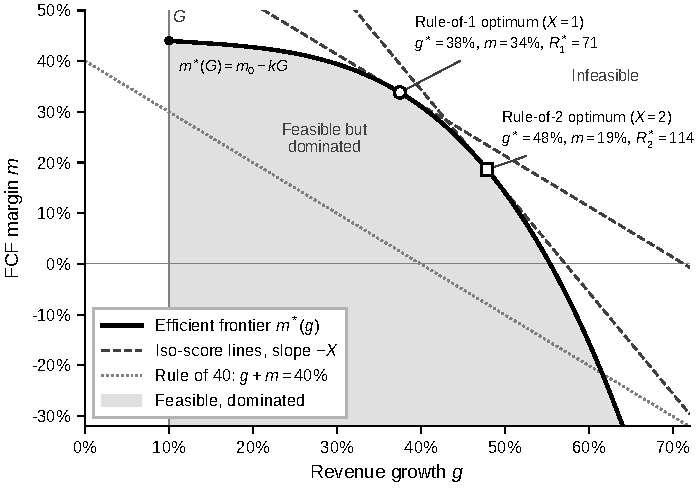
\includegraphics[width=0.64\linewidth]{figures/fig_frontier_tangency.pdf}
\caption{The efficient frontier and the Rule of $X$. The solid curve is the frontier $m^*(g)$ of \autoref{prop:frontier} for $m_0=0.45$, $G=0.10$, $k=0.10$, $\alpha=0.3$ and $\ell=0.6$; the shaded area is the set of feasible but dominated points. The dotted line is the Rule-of-40 boundary $g+m=0.40$. The dashed lines are iso-score lines of slope $-1$ and $-2$, tangent to the frontier at the Rule-of-1 and Rule-of-2 optima (markers) characterized in \autoref{prop:score}.}\label{fig:frontier}
\end{figure}

\subsection{The Rule of \texorpdfstring{$X$}{X} as a supporting line}\label{sec:model-score}

Geometrically, the frontier is a transformation curve between growth and margin, and a Rule-of-$X$ score is a price line with slope $-X$; its level sets are iso-score lines, not iso-value lines (\autoref{prop:general}(c)). The tangency between the two has antecedents in the growth-valuation frontier of the managerial firm \citep{marris1964economic,solow1971some,odagiri1981theory}, and recent firm-level evidence that firms grow by acquiring customers through marketing and distribution at roughly constant markups supports the growth technology behind it \citep{fitzgerald2024how,argente2025how,afrouzi2023concentration}. Given the functional form, the closed forms below are a routine power-function calculation.

\begin{lemma}[Maximal Rule-of-$X$ score]\label{prop:score}\label{prop:optimum}
Fix $X\ge 0$ and $s$. In parts (b) and (e), assume that the financing cap does not bind, that is, $\sigma^*\le\bar\sigma$ with $\sigma^*$ given in \eqref{eq:sigstar}; this always holds if $\bar\sigma=\infty$.
\begin{enumerate}
\item[(a)] Iso-score sets $\{(g,m):Xg+m=c\}$ are straight lines of slope $-X$. A maximizer of $R_X$ on $\mathcal F$ exists, and every maximizer lies on the frontier.
\item[(b)] If $X>k$, the maximizer is unique and interior ($g^*>G$), and there the frontier is tangent to the iso-score line: $m^{*\prime}(g^*)=-X$ (if $\sigma^*=\bar\sigma$, the maximizer is the right endpoint $\bar g$ of $I$ and the tangency holds for the left derivative). In closed form,
\begin{align}
\Delta^* &= g^*-G=(\lambda h)^{1/(1-\alpha)}\,\bigl[\alpha(X-k)\bigr]^{\alpha/(1-\alpha)}, \label{eq:Dstar}\\
\sigma^* &= \bigl[\alpha\lambda h\,(X-k)\bigr]^{1/(1-\alpha)} \;=\; \alpha(X-k)\,\Delta^*, \label{eq:sigstar}\\
R_X^* &= m_0+(X-k)\,G+(1-\alpha)(X-k)\,\Delta^* \;=\; m_0+(X-k)\,G+C_\alpha\bigl[\lambda h\,(X-k)\bigr]^{1/(1-\alpha)}, \label{eq:Rstar}
\end{align}
and the margin at the optimum is $m^*(g^*)=m_0-kg^*-\alpha(X-k)\Delta^*$.
\item[(c)] If $X\le k$, the unique maximizer is the corner $g^*=G$ with $\sigma^*=0$, and $R_X^*=m_0+(X-k)G$. This part does not need the cap condition.
\item[(d)] (Duality.) Each frontier point with $G<g<\bar g$ is the unique maximizer of $R_X$ for exactly one weight, $X(g)=-m^{*\prime}(g)=k+\beta\kappa(g-G)^{\beta-1}$. The point $g=G$ is a maximizer if and only if $X\le k$. If $\bar\sigma=\infty$, the optimal growth rate $g^*(X)$ is continuous and nondecreasing in $X$, and strictly increasing for $X>k$.
\item[(e)] The growth surplus $\Pi:=(1-\alpha)(X-k)\Delta^*$ (zero if $X\le k$) satisfies $\Pi=\max_{\sigma\ge 0}\{(X-k)\,\ell\,\sigma^{\alpha}-\sigma\}$, so that $R_X^*=m_0+(X-k)G+\Pi$.
\end{enumerate}
\end{lemma}

When the dependence matters we write $\Delta^*(\ell,X)$ and $\sigma^*(\ell,X)$ for \eqref{eq:Dstar} and \eqref{eq:sigstar} with $\lambda h$ replaced by $\ell$ and $X-k$ by $(X-k)_+$.

\noindent\emph{Intuition.} Because the feasible set is convex, maximizing a linear score is a supporting-line problem: push a line of slope $-X$ outward until it last touches the frontier. The maximal score has three parts. The intercept $m_0$ is what the firm earns without outgrowing its market. The term $(X-k)G$ is the value of the free growth the market supplies, net of the capital it requires. The growth surplus $\Pi$ is the profit from running the growth technology at a shadow price of $X-k$ per unit of growth. The spend rule $\sigma^*=\alpha(X-k)\Delta^*$ is a \citet{dorfman1954optimal} condition: spend equals the spend elasticity times the value of the growth it buys, so the fraction $\alpha$ of that value is spent and the fraction $1-\alpha$ is kept as surplus. When the weight on growth does not cover the capital each unit of growth needs ($X\le k$), the firm should buy no growth. Part (d) says the weight $X$ indexes the frontier: choosing a rule is the same as choosing a point.

Remarks~\ref{rem:cap} and \ref{rem:r40} in the Supplementary Appendix treat a binding financing cap and show that the Rule of 40, read as a pass mark, accepts an interval of frontier points and dominated points below them, whereas the Rule of $X$ selects one. \autoref{rem:general-phi} separates the results that hold for any increasing concave growth technology from those specific to the isoelastic form \eqref{eq:growth}.

\subsection{Limits: saturation, small base and the score budget}\label{sec:model-limits}

Write $R_X^*(s)$ for the maximal score at share $s$ when $\bar\sigma=\infty$, let $y_+:=\max\{X-k,0\}$, and define the saturated score
\begin{equation}\label{eq:Rinf}
R_\infty:=m_0+(X-k)\,G .
\end{equation}

\begin{lemma}[Saturation and the small-base bound]\label{prop:saturation}
Fix $X\ge 0$ and let $\bar\sigma=\infty$.
\begin{enumerate}
\item[(a)] $R_X^*(s)=R_\infty+C_\alpha\bigl[\lambda h(s)\,y_+\bigr]^{1/(1-\alpha)}$. If $X>k$, this is strictly decreasing in $s$, with $dR_X^*/ds=-(X-k)\Delta^*/(\bar s-s)$. If $X\le k$, it is constant.
\item[(b)] (Saturation limit.) $\lim_{s\to\bar s}R_X^*(s)=R_\infty$. For the Rule of 40 with $k=0$, the limit is $m_0+G$. Since $m_0=1-c_h-c_c-f-a\le 1-c_c-f-a_{\min}\le 1$,
\begin{equation}\label{eq:rule100}
R_\infty\;\le\;1-c_c-f-a_{\min}+(X-k)\,G,\qquad\text{and for }X=1:\quad R_\infty\le 1+(1-k)\,G .
\end{equation}
\item[(c)] (Small-base bound.) $\sup_{s\in(0,\bar s)}R_X^*(s)=\lim_{s\to 0}R_X^*(s)=R^0:=R_\infty+C_\alpha(\lambda y_+)^{1/(1-\alpha)}$. If $X>k$, the supremum is not attained; if $X\le k$, $R_X^*$ is constant in $s$ and the supremum is attained at every share.
\item[(d)] (Demand-pull threshold.) Let $X>k$ and $\bar R>R_\infty$, and define
\begin{equation}\label{eq:Lambda}
\Lambda(\bar R):=\frac{1}{X-k}\left[\frac{\bar R-R_\infty}{C_\alpha}\right]^{1-\alpha}.
\end{equation}
Then $R_X^*(s)\ge\bar R$ if and only if $\lambda h(s)\ge\Lambda(\bar R)$, and a score of $\bar R$ is attainable at some share if and only if $\lambda>\Lambda(\bar R)$. A firm exactly at the threshold has $\Delta^*=(\bar R-R_\infty)/[(1-\alpha)(X-k)]$, $\sigma^*=\alpha(\bar R-R_\infty)/(1-\alpha)$ and $m=m_0-kg^*-\sigma^*$.
\end{enumerate}
\end{lemma}

\noindent\emph{Intuition.} Rising share uses up growth opportunity. As $s\to\bar s$, the growth surplus vanishes and the best score falls to the margin intercept plus the value of free market growth. Because the margin intercept cannot exceed 100\% of revenue, a saturated firm with negligible capital cannot sustain a Rule-of-40 score above $100(1+G)$ points. With $G$ between 0.05 and 0.30, this is the formal content of a ``Rule of about 100''. Scores far above that level need demand pull above the threshold \eqref{eq:Lambda}, and even then only at small share, with very large spend and deeply negative margins. With $\alpha=0.3$, $X=1$, $k=0$, $m_0=0.6$ and $G=0.2$ ($R_\infty=0.8$), a ``Rule of 1000'' requires $\lambda h\ge\Lambda\approx 8.71$; at the threshold the firm grows about 1{,}314 points faster than its market, spends about 394\% of revenue on growth and runs an FCF margin of about $-334\%$, in continuously compounded rates. \autoref{prop:myopic} in the Supplementary Appendix adds that, if the firm spends at the static optimum for a fixed weight at every date (a myopic policy, not the dynamically optimal one of \autoref{prop:dynamic}), its excess over $R_\infty$ decays at least as fast as $t^{-1/\alpha}$.

\begin{figure}[t]
\centering
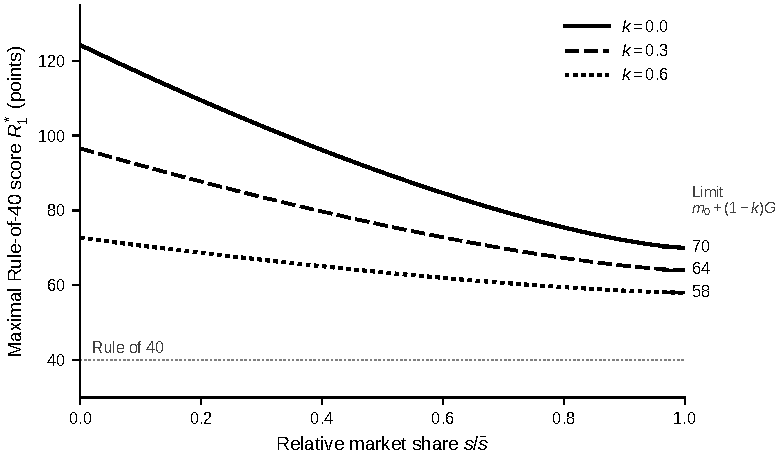
\includegraphics[width=0.64\linewidth]{figures/fig_saturation.pdf}
\caption{Saturation. The maximal Rule-of-40 score $R_1^*$ of \autoref{prop:saturation}(a) as a function of the relative share $s/\bar s$, for capital intensities $k\in\{0,0.3,0.6\}$, with $m_0=0.50$, $G=0.20$, $\lambda=1.2$ and $\alpha=0.3$. Each curve falls to its saturation limit $m_0+(1-k)G$, marked by a horizontal tick and label at the right edge. The dotted line marks a score of 40.}\label{fig:saturation}
\end{figure}

The next result makes the transience of extreme scores precise. It needs neither the functional form \eqref{eq:growth} nor optimal behavior. It needs the margin bound $m\le m_0-kg$, growth of at least $G$ at every spend level (no share is lost without spend), and share accounting in a single market whose size grows exogenously at $G$ under a fixed cap $\bar s$.

\begin{proposition}[Score budget]\label{prop:budget}
Let the firm sell in a single market whose size grows exogenously at rate $G$, with a fixed share cap $\bar s$, and let its growth be at least $G$ whatever its spend. Hold $m_0$, $G$, $k$ and $X>k$ fixed, and let $R_\infty=m_0+(X-k)G$.
\begin{enumerate}
\item[(a)] (Continuous time.) Take any measurable spend path $\sigma:[0,T]\to[0,\bar\sigma]$ with $\int_0^T\sigma^{\alpha}\,dt<\infty$, any measurable margins $m(t)\le m_0-\sigma(t)-k\,g(t)$, and the induced share path from $s(0)=s_0$. Then
\begin{equation}\label{eq:budget}
\int_0^T\bigl(R_X(t)-R_\infty\bigr)^+\,dt\;\le\;(X-k)\,\ln\frac{s(T)}{s_0}\;<\;(X-k)\,\ln\frac{\bar s}{s_0}.
\end{equation}
\item[(b)] (Discrete time.) Suppose instead that growth and margins are period rates, with $G>-1$: $s_{t+1}=s_t(1+g_t)/(1+G)$, $g_t\ge G$, $m_t\le m_0-kg_t$, and $s_t\le\bar s$ for all $t$. Then
\begin{equation}\label{eq:budget-discrete}
\sum_{t=0}^{T-1}\ln\!\Bigl(1+\frac{(R_{X,t}-R_\infty)^+}{(X-k)(1+G)}\Bigr)\;\le\;\ln\frac{s_T}{s_0}\;\le\;\ln\frac{\bar s}{s_0}.
\end{equation}
\item[(c)] (Moving intercept.) If the margin intercept moves over time, $m_0(t)$, then (a) and (b) hold with $R_\infty(t)=m_0(t)+(X-k)G$ in place of $R_\infty$.
\end{enumerate}
\end{proposition}

\noindent\emph{Intuition.} Every point of score above the saturated level must be paid for with excess growth, and excess growth is share growth. Share can grow only from $s_0$ to $\bar s$, so the log headroom $\ln(\bar s/s_0)$ is a finite budget that every growth strategy draws on. A firm can spend the budget quickly, on a high but brief score, or slowly, on a modest but long-lived one; \autoref{prop:budget-sharp} in the Supplementary Appendix shows that the bound \eqref{eq:budget} is sharp, and is approached only by slow spending: a firm that spends fast converts headroom into score at a lower rate, because spend rises more than proportionally with excess growth (\autoref{cor:transient}(b)). Within one market, and with zero-spend growth at least equal to market growth, a firm cannot spend the budget twice. The budget is finite only under those conditions: a firm whose retention lags its market loses share without spending and can buy it back repeatedly (\autoref{rem:assumptions}(b)), a firm that acquires businesses in markets it does not yet serve buys new headroom with each deal (\autoref{prop:acquired-score}(e)), and a firm that creates a new market with a new product opens a new budget in that market. The proposition bounds score per market at given retention, not the score of a firm that keeps entering markets.

\begin{corollary}[Extreme scores are transient]\label{cor:transient}
Let $X>k$ and $\bar R>R_\infty$.
\begin{enumerate}
\item[(a)] (Period rates.) In the setting of \autoref{prop:budget}(b), the number $\mathcal T(\bar R)$ of periods in which a firm starting at share $s_0$ scores at least $\bar R$ satisfies
\begin{equation}\label{eq:transient}
\mathcal T(\bar R)\;\le\;\frac{\ln(\bar s/s_0)}{\ln\bigl(1+(\bar R-R_\infty)/[(X-k)(1+G)]\bigr)} .
\end{equation}
\item[(b)] (Continuous time.) In the setting of \autoref{prop:budget}(a), the time a firm spends at or above $\bar R$ is at most $(X-k)\ln(\bar s/s_0)/(\bar R-R_\infty)$. Under the growth technology \eqref{eq:growth}, a firm that sets spend at the static optimum for the weight $X$ at every date (\autoref{prop:myopic}) spends at most $(1-\alpha)(X-k)\ln(\bar s/s_0)/(\bar R-R_\infty)$ there.
\end{enumerate}
For example, let $X=1$, $k=0$, $m_0=0.6$ and $G=0.2$ (so $R_\infty=0.8$), with $\bar s=0.5$. In annual periods, from $s_0=1\%$ the firm can score at least 1{,}000 points ($R_1\ge 10$) in at most one year (the bound is 1.8) and at least 140 points in at most nine years (bound 9.6); from $s_0=10^{-5}$ it can score at least 1{,}000 points in at most five years (bound 5.0). In continuous time, from $s_0=1\%$ it can score at least 1{,}000 points for at most 0.43 years, and for at most 0.30 years at the static optimum.
\end{corollary}

\subsection{Comparative statics}\label{sec:model-statics}

\begin{lemma}[Envelope results]\label{prop:envelope}\label{prop:capital}
Let $\bar\sigma=\infty$ and $X\ge 0$. The maximal score $R_X^*$ is continuously differentiable in $(m_0,G,k,X,\lambda,s)$, with
\begin{equation}\label{eq:envelope}
\begin{gathered}
\frac{\partial R_X^*}{\partial m_0}=1,\qquad
\frac{\partial R_X^*}{\partial G}=X-k,\qquad
\frac{\partial R_X^*}{\partial k}=-g^*,\qquad
\frac{\partial R_X^*}{\partial X}=g^*,\\
\frac{\partial R_X^*}{\partial\lambda}=\frac{(X-k)\Delta^*}{\lambda}=(X-k)\,h\,(\sigma^*)^{\alpha}\ge 0,
\end{gathered}
\end{equation}
where the last inequality is strict if and only if $X>k$. Through $m_0=\gamma-a$ and $\gamma=1-c_h-c_c-f$, $\partial R_X^*/\partial\gamma=1$ and $\partial R_X^*/\partial a=\partial R_X^*/\partial c_c=-1$. Moreover $R_X^*$ is convex in $k$ and in $\lambda$, and $\partial^2R_X^*/\partial k\,\partial\lambda=-\Delta^*/[(1-\alpha)\lambda]\le 0$.
\end{lemma}

\noindent\emph{Intuition.} By the envelope theorem, a parameter change can be valued at the optimal point without re-optimizing. Capital intensity is charged on every unit of growth, including the free market growth, so its marginal cost is the growth rate itself. The negative cross-partial says that firms with more growth opportunity are hurt more by capital intensity.

\begin{corollary}[Capital-for-labor substitution]\label{cor:capital}\label{cor:substitution}
Let $\bar\sigma=\infty$, and suppose automation lowers $a$ by $da>0$ and raises $k$ by $dk>0$, with other parameters fixed. Then the change in the maximal score satisfies
\begin{equation}\label{eq:kl-bracket}
da-g^*(k)\,dk\;\le\;\Delta R_X^*\;\le\;da-g^*(k+dk)\,dk .
\end{equation}
Hence the score rises if $da>g^*(k)\,dk$ and does not rise if $da\le g^*(k+dk)\,dk$. To first order, it rises if and only if $da>g^*\,dk$.
\end{corollary}

\noindent\emph{Intuition.} Replacing recurring human cost with owned capital raises the FCF score only if the opex saved per dollar of revenue exceeds the growth rate times the added capital per dollar of revenue, because the capital must be bought again for every new dollar of revenue. Without depreciation, raising $k$ by 0.10 must cut opex by more than 5 points of revenue for a firm growing at 50\%, but by only 1 point for a firm growing at 10\%. Compute depreciates quickly, however: with depreciation at rate $\delta_K$ the threshold becomes $(g^*+\delta_K)\,dk$ (\autoref{rem:assumptions}(c)), so at $\delta_K=0.25$ the two figures rise to 7.5 and 3.5 points. The bracket \eqref{eq:kl-bracket} holds exactly, not only to first order, because $R_X^*$ is convex in $k$.

\begin{corollary}[Automation priorities]\label{cor:priorities}
Let $\bar\sigma=\infty$ and $X>k$, so that the Rule-of-$X$ optimum is interior, and evaluate each improvement at the optimum, with spend re-optimized and the weight $X$ held fixed. To first order:
\begin{enumerate}
\item[(i)] (Non-discretionary cost.) Removing non-discretionary cost $da$ (a share of revenue) raises $R_X^*$ by $da$ and the saturated score $R_\infty$ by $da$, so the gain survives saturation.
\item[(ii)] (Growth engine.) Let an improvement $x$ in the efficiency of growth spend deliver the same growth for spend $\sigma/(1+x)$, which maps to $\lambda\mapsto\lambda(1+x)^{\alpha}$. It raises $R_X^*$ by $x\,\sigma^*$, the same as cutting a non-discretionary cost line of size $\sigma^*$ by the proportion $x$; exactly, by $\Pi[(1+x)^{\alpha/(1-\alpha)}-1]$. Measured instead as a rise $x_\lambda$ in demand pull, the gain is $x_\lambda(X-k)\Delta^*=x_\lambda\,\sigma^*/\alpha$ to first order and $\Pi[(1+x_\lambda)^{1/(1-\alpha)}-1]$ exactly; the factor $1/\alpha$ between the two reflects only the unit in which the improvement is measured. Neither raises $R_\infty$, and both vanish as $s\to\bar s$.
\item[(iii)] (Retention.) Raising zero-spend growth $G_i$ (net revenue retention, \autoref{rem:assumptions}(b)) by $dG$ raises $R_X^*$ by $(X-k)\,dG$, and $R_\infty$ by the same amount; at a fixed weight the gain does not depend on the firm's share or growth.
\item[(iv)] (Cost of revenue.) A cut $du<0$ in unit cost of revenue raises the gross margin, and hence $R_X^*$, by $(1-\epsilon_p)|du|/p$ at given demand, where $\epsilon_p$ is the pass-through elasticity of \autoref{lem:prices}. Under free entry without a scarce input it leaves the long-run markup at zero (\autoref{prop:entry}(b)); the long-run score then changes only through the normal return on capital and customer capital, $(r-G)(k_u+a_c)/\hat c$, because lower prices raise capital per dollar of revenue, and not at all if $k_u+a_c=0$.
\item[(v)] (Capital for labor.) Automation that adds capital $dk$ while removing cost $da$ raises $R_X^*$ if and only if $da>g^*dk$ (\autoref{cor:capital}); since $g^*\ge G$, the hurdle is lowest for the slowest growers.
\end{enumerate}
\end{corollary}

\noindent\emph{Intuition.} At a fixed weight, the gain from cutting non-discretionary cost survives saturation (part (i)), the gain from a better growth engine vanishes with it (part (ii)), savings in cost of revenue count only to the extent the firm keeps them (part (iv)), and capital-heavy automation suits slow growers (part (v)). A ranking by stage needs one more step. If the firm acts on its own decision weight $X^{\mathrm{dyn}}(s)=v'(s)$ of \autoref{prop:dynamic}, which in the worked example there falls from \VpOnePct{} at 1\% of the cap to about \VpMin{} near \VpMinAt\% and stays below its small-share values up to saturation, then the gains in (ii) and (iii), both proportional to $X-k$, are larger for a firm at small share, although near saturation the retention gain of (iii) is still about \VpGainShare\% of its small-share value; at a common fixed weight, only the saturation of (ii) distinguishes stages. Parts (i) and (iii) treat cost and retention as independent levers, but spending on customer success and support sits in $a$ and sustains retention, so cutting it may lower $G_i$. These are effects that shift the frontier itself, distinct from closing a firm's distance to its frontier.

\subsection{Which weight on growth? The firm's and the investor's}\label{sec:model-valuation}

The score results take the weight $X$ as given. Which weight should a firm use, and how does it relate to the weights of 2 to 3 in investors' screens? We answer the first question with the firm's dynamic problem and the second with a valuation identity. Both weights turn out to be marginal rates of substitution between growth and margin in value; they price perturbations of different persistence. The dynamic problem belongs to the class of optimal-advertising problems with a saturating sales response \citep{sethi1973optimal,sethi1977dynamic,feichtinger1994dynamic}, in which the costate is the marginal value of sales, and the firm's weight is the counterpart of the shadow value of customer capital \citep{gourio2014customer} or brand capital \citep{vitorino2014understanding} in models of marketing as investment; in the investment model of \citet{belo2022decomposing}, brand capital accounts for 6\% to 25\% of firm value, depending on the industry. What we add is the reading of the optimum, under (H), as a Rule-of-$X$ score at every date and the comparison of that weight with the weights investors screen on.

Let $r>G$ be the discount rate. A spend policy is a measurable $\sigma:[0,\infty)\to[0,\infty)$ with $\int_0^t\sigma^{\alpha}d\tau<\infty$ for all $t$. Under Assumptions~\ref{ass:market}--\ref{ass:capital} it induces, from $s(0)=s_0$, the share path $\dot s=s\,\ell(s)\,\sigma^{\alpha}$ with $\ell(s)=\lambda h(s)$, revenue $S_t=s_tM_t$ and FCF margin $m_t=m_0-\sigma_t-kg_t$. Firm value is
\begin{equation}\label{eq:value}
V(S_0,M_0):=\sup_{\sigma}\ \limsup_{T\to\infty}\int_0^Te^{-rt}\,m_t\,S_t\,dt,
\end{equation}
where each integral is well defined in $[-\infty,\infty)$ because $m_t\le m_0-kG$.

\begin{proposition}[Dynamic optimality: under (H), the firm's own growth weight is the marginal $q$ of revenue]\label{prop:dynamic}
Let $\bar\sigma=\infty$, $r>G$ and $m_0-kG>0$.
\begin{enumerate}
\item[(a)] (Homogeneity.) $V(S,M)=M\,v(S/M)$, where $v(s):=V(s,1)$ satisfies $(m_0-kG)\,s/(r-G)\le v(s)\le(m_0-kG)\,\bar s/(r-G)$. Hence $\partial V/\partial S=v'(s)$, the marginal value of a dollar of revenue, and $V/S=v(s)/s$, the revenue multiple, wherever $v$ is differentiable.
\item[(b)] (Verification.) Let $\hat v\in C^1((0,\bar s))$ be bounded and satisfy the Hamilton--Jacobi--Bellman (HJB) equation
\begin{equation}\label{eq:hjb}
(r-G)\,\hat v(s)\;=\;s\max_{\sigma\ge 0}\bigl\{m_0-\sigma-kG+\bigl(\hat v'(s)-k\bigr)\,\ell(s)\,\sigma^{\alpha}\bigr\}\qquad\text{for all }s\in(0,\bar s).
\end{equation}
Then $\hat v\ge v$. Say that the verification hypothesis (H) holds if such a $\hat v$ exists and, from every $s_0\in(0,\bar s)$, the feedback $\hat\sigma(s)=\sigma^*(\ell(s),\hat v'(s))$ generates a share path in $(0,\bar s)$. Under (H), $\hat v=v$ and the feedback is optimal.
\item[(c)] (The Rule of $X$ at every date.) The maximand in \eqref{eq:hjb} equals $R_X(g,m)-XG$ with $X=\hat v'(s)$. Under (H), a firm that follows the optimal feedback therefore maximizes, at every date, the Rule-of-$X$ score at its current share, with weight
\begin{equation}\label{eq:Xdyn}
X^{\mathrm{dyn}}(s)\;=\;v'(s)\;=\;\frac{\partial V}{\partial S},
\end{equation}
the marginal $q$ of revenue; and \eqref{eq:hjb} can be written $R^*_{X^{\mathrm{dyn}}(s)}(s)=(r-G)\,v(s)/s+G\,X^{\mathrm{dyn}}(s)$.
\item[(d)] (Small share.) Let $v_0$ be the smallest positive number that satisfies
\begin{equation}\label{eq:gordon}
(r-G)\,v_0\;=\;m_0-kG+C_\alpha\bigl[\lambda\,(v_0-k)_+\bigr]^{1/(1-\alpha)},
\end{equation}
assumed to exist and to be a simple root, and let $\Delta^\circ=\Delta^*(\lambda,v_0)$, $\sigma^\circ=\sigma^*(\lambda,v_0)$, $g^\circ=G+\Delta^\circ$ and $m^\circ=m_0-kg^\circ-\sigma^\circ$. Then $g^\circ<r$ and $v_0=m^\circ/(r-g^\circ)$; $v(s)\le v_0\,s$ for all $s$; and $\lim_{s\to 0}v(s)/s=v_0$. Under (H), also $X^{\mathrm{dyn}}(s)=\hat v'(s)\to v_0$ as $s\to 0$.
\item[(e)] (No root.) If \eqref{eq:gordon} has no positive root, then $v(s)/s\to\infty$ as $s\to 0$.
\end{enumerate}
\end{proposition}

Parts (a), (d) and (e) hold unconditionally; parts (b) and (c) state what follows if (H) holds. We have not proved (H). It is the hypothesis of a verification theorem, and we state it as an assumption. Where spend is positive, \eqref{eq:hjb} is equivalent to an explicit first-order ordinary differential equation in $v$ that is singular at both ends of $(0,\bar s)$ (Section~\ref{app:proofs} of the Supplementary Appendix). For the parameters of the worked example below, a numerical solution of \eqref{eq:hjb} by dynamic programming on a fine grid has a smooth profile, and its feedback generates admissible paths (\texttt{code/verify\_theory.py}, checks 15g to 15m). That is evidence for (H) at those parameters, not a proof. Two consequences of \eqref{eq:hjb} show what (H) requires. If $(m_0-kG)/(r-G)\le k$, the linear function $\hat v(s)=(m_0-kG)s/(r-G)$ solves \eqref{eq:hjb}, so (H) holds and the firm never spends on growth. If $(m_0-kG)/(r-G)>k$, no solution has a region without spend, so under (H) the firm spends at every share, and $\hat v$ must meet the terminal condition $\hat v(\bar s)=(m_0-kG)\bar s/(r-G)$; the numerical solution passes through that singular point. The second condition of (H), that the feedback generates a share path, then holds automatically, so the content of (H) is the existence of a bounded continuously differentiable solution of \eqref{eq:hjb} on $(0,\bar s)$. Every statement in this paper that a value-maximizing firm acts on a weight equal to the marginal value of revenue is conditional on (H).

\noindent\emph{Intuition.} A point of excess growth bought today is a permanent addition to the revenue base, worth $v'(s)$ per dollar of revenue, while the spend that buys it is paid once. Under (H), the HJB equation splits the firm's problem into a sequence of static Rule-of-$X$ problems, one per date, with a weight equal to the marginal value of revenue. The Rule of $X$ is then the right instantaneous criterion, and its weight is a marginal value of revenue, not a fixed 2 or 3. \citet{hayashi1982tobin} shows that marginal and average $q$ coincide when value is linearly homogeneous in the stock. Here value is homogeneous of degree one in revenue and market size jointly, not in revenue alone, so saturation drives marginal $q$ of revenue, $v'(s)$, apart from the revenue multiple $v(s)/s$. The two coincide in the small-share limit of part (d), where the firm is a constant-growth firm whose revenue multiple $v_0=m^\circ/(r-g^\circ)$ is the Gordon multiple. Part (e) is the case in which the growth technology allows growth at a rate close to the discount rate with a positive margin, so that the small-share multiple is unbounded.

\noindent\emph{Worked example.} In the example of Section~\ref{supp:model-weights} of the Supplementary Appendix, under (H), a firm whose revenue multiple at a small share is 10 acts on a growth weight of \VpOnePct, \VpTenPct{} and \VpFiftyPct{} at 1\%, 10\% and 50\% of its share cap, close to and below its revenue multiple; the weight falls to about \VpMin{} near \VpMinAt\% of the cap and then rises toward the never-spend multiple of \VpLimit; a multiple of 15 gives correspondingly higher weights. In the example the weight lies below the revenue multiple at every share, so the firm's own weight exceeds the screening weights of 2 to 3 when its revenue multiple is well above three; at a higher discount rate both are lower.

\noindent\emph{Implication for measurement.} Because $\sigma^*=\alpha(X-k)\Delta^*$, the ratio of growth spend to excess growth over market growth reveals $\alpha(X-k)$, and since $\alpha<1$ it bounds the net weight from below whatever $\alpha$ is: $X-k=(\sigma^*/\Delta^*)/\alpha>\sigma^*/\Delta^*$. Conditional on $\alpha$, a spend ratio $\hat\rho$ implies $X-k=\hat\rho/\alpha$, between $2.2\hat\rho$ and $4\hat\rho$ for $\alpha\in[0.25,0.45]$. The data observe neither growth spend nor excess growth over market growth. The selling-and-marketing share also contains spending that maintains revenue, and excess growth is measured against the sample median rather than against $G$. Section~\ref{sec:empirics} reports the values of $\alpha(X-k)$ that different proxies give: from \AlphaAllLo{} to \AlphaAllHi{} across methods, so that $X-k$ ranges from about \XkLo{} to about \XkHi{} for $\alpha\in[0.25,0.45]$. The spend data therefore do not identify the decision weight. Under (H), whether a firm's decision weight exceeds the screening weights is therefore a statement about its revenue multiple (part (c) and the worked example), not a finding from spending data. Where an example below needs a weight, we evaluate it at $X\in\{2.5,5,9\}$ and say where its conclusion changes below 2.5.

The weights in investors' screens answer a different question. They compare a change in the growth rate that persists for several years with a change in the margin, which is what regressions of revenue multiples on growth and margin estimate. Let $\eta:=(1+g)/(1+r)$, $\mathcal N_T(\eta):=\sum_{t=1}^T\eta^t$, and let $\mathcal M_\infty:=(1+G_\infty)/(r-G_\infty)$ be a Gordon multiple for growth $G_\infty\in(-1,r)$ after year $T$.

\begin{lemma}[The investor's screening weight]\label{lem:valuation2}\label{lem:valuation}\label{lem:ruleX}
Let $V=S_0\,[\,m\,\mathcal N_T(\eta)+m_{LR}\,\eta^T\mathcal M_\infty\,]$: revenue grows at $g$ for $T$ years and at $G_\infty$ thereafter, the current margin $m$ holds for $T$ years, and the long-run margin is $m_{LR}=\theta m+(1-\theta)\bar m$, where $\theta\in[0,1]$ measures the persistence of the current margin and $\bar m$ is the margin the business earns at maturity. Define $X^{\mathrm{scr}}:=(\partial V/\partial g)/(\partial V/\partial m)$.
\begin{enumerate}
\item[(a)] In general,
\begin{equation}\label{eq:X2}
X^{\mathrm{scr}}=\frac{m\sum_{t=1}^Tt\,\eta^t+m_{LR}\,T\,\eta^T\mathcal M_\infty}{(1+g)\bigl[\mathcal N_T(\eta)+\theta\,\eta^T\mathcal M_\infty\bigr]} .
\end{equation}
\item[(b)] (Persistent margin.) If $\theta=1$ and $\mathcal M_\infty=0$, then
\begin{equation}\label{eq:XmD}
X^{\mathrm{scr}}=\frac{m\,D}{1+g},\qquad D:=\frac{\sum_{t=1}^Tt\,\eta^t}{\sum_{t=1}^T\eta^t},
\end{equation}
where $D$ is the present-value-weighted average date (Macaulay duration) of the revenue stream. $D$ is strictly increasing in $T$; for $T\ge 2$ it is strictly increasing in $g$ and strictly decreasing in $r$; and $D=1$ for $T=1$. If $\theta=1$ and $\mathcal M_\infty>0$, the same formula holds with $D$ replaced by $D_{TV}:=[\sum_{t=1}^Tt\,\eta^t+T\eta^T\mathcal M_\infty]/[\mathcal N_T(\eta)+\eta^T\mathcal M_\infty]$.
\item[(c)] (Transitory margin.) If $\theta<1$ and $\bar m>0$, then $X^{\mathrm{scr}}>0$ even when $m=0$. If $0\le m\le\bar m$ and $\bar m>0$, then $X^{\mathrm{scr}}$ is strictly decreasing in $\theta$.
\item[(d)] (Gordon limit.) If $\theta=1$, $\mathcal M_\infty=0$ and $g<r$, then as $T\to\infty$, $X^{\mathrm{scr}}\to m(1+r)/[(1+g)(r-g)]=(V/S_0)\,(1+r)/(1+g)^2$.
\item[(e)] (One-period trade.) If $T=1$ and $\theta=0$, so that the growth rate is raised and the margin lowered for one period only, then $X^{\mathrm{scr}}=(m+\bar m\,\mathcal M_\infty)/(1+g)=(V/S_0)\,(1+r)/(1+g)^2$.
\end{enumerate}
\end{lemma}

The screening weight is a duration, as in the implied equity duration of \citet{dechow2004implied}; Section~\ref{supp:model-weights} of the Supplementary Appendix evaluates it for typical parameters.

The two weights are therefore the same object, a marginal rate of substitution between growth and margin in value, evaluated for perturbations of different persistence. The firm's decision concerns a one-period trade: spend this period buys a permanent addition to revenue and costs margin once. For that trade part (e) gives $X^{\mathrm{scr}}=(V/S_0)(1+r)/(1+g)^2$, the discrete-time counterpart of the decision weight $X^{\mathrm{dyn}}=v'(s)$ in the small-share limit of \autoref{prop:dynamic}(d), where $v'(s)\to v_0=V/S$. Regressions of revenue multiples on growth and margin compare persistent differences in growth and margin across firms, which corresponds to $T$ of several years and $\theta$ near one; there the weight is a duration-scaled margin of the order of 1 to 3. Over $(T,\theta)$ the screening weight spans more than an order of magnitude, so a weight of 2 to 3 reflects a choice of persistence, not a prediction of the model. Under (H), a firm that maximized a score with a weight below its decision weight would buy too little growth, because $\Delta^*$ is increasing in $X$ (\autoref{prop:score}(d)). The screening weight also has the usual limits of a local approximation: it varies with $r$, $T$, $\theta$ and the margin level, and it ignores risk, dilution from stock-based compensation and the gap between GAAP and FCF margins.

% FRONTIER-SLOPE placeholders: paper1/macros.tex (generated) defines these once the Psi_chi slopes are adopted; \providecommand leaves a generated definition untouched.
\providecommand{\PsiSlopeOp}{\textbf{[$\Psi_\chi$ slope, GAAP]}}
\providecommand{\PsiSlopeCash}{\textbf{[$\Psi_\chi$ slope, cash]}}
\subsection{Heterogeneous firms: the industry frontier as an upper envelope}\label{sec:model-industry}

Empirical frontiers are drawn across firms. Section~\ref{sec:empirics} estimates the slope of the $\chi$-quantile frontier $\Psi_\chi$ of \autoref{def:industry}, the $\chi$-quantile of the margin among firm-years growing at least $g$, at $-$\PsiSlopeOp{} on the GAAP basis and $-$\PsiSlopeCash{} after stock-based compensation, and finds a within-firm slope near zero. % FRONTIER-SLOPE: \PsiSlopeOp and \PsiSlopeCash are placeholders for the Psi_chi slopes (absolute values) of notes/frontier_slope_v3.json; see notes/theory_fixes_v2.md for the exact estimand (chi, window, basis, sample).
That section also reports the local conditional quantile of the margin given growth near $g$. It is a different, descriptive object: it conditions on growth near $g$ rather than at least $g$, and the results below speak to $\Psi_\chi$, not to it. This subsection shows what each fact can and cannot reveal. The cross-sectional slope is consistent with two different structures. One is a common frontier, on which firms that act on different weights choose different points; under it the estimated slope maps into the frontier's parameters, and, evaluated at the sample's growth distribution, the frontier's steepest slope in the window is between \PsiMultLo{} and \PsiMultHi{} times the estimated slope for $\alpha\in[0.25,0.45]$, or \PsiSteepConeLo{} to \PsiSteepConeHi{} on the two bases (Section~\ref{supp:model-slope} of the Supplementary Appendix). Read literally, this structure places firms at different points of one frontier, which requires them to act on different weights, none above that steepest slope. The other is selection by quality, in which firms with more growth opportunity also have higher margin intercepts (part (ii) below). The cross-section cannot tell these apart (part (iv)). If firms act on weights above the steepest slope of a common frontier, as they would if their decision weights were close to their revenue multiples (\autoref{prop:dynamic}), only the second structure fits. The within-firm slope requires more (part (v)): anticipated shocks to opportunity would make it negative for every weight above $k$, so unanticipated demand shocks or costs committed in advance must offset them.

\begin{assumption}[Heterogeneous firms]\label{ass:hetero}
A set $\mathcal I$ of firms shares $G\ge 0$, $\alpha$, $X\ge 0$ and a finite financing cap $\bar\sigma<\infty$. Firm $i$ has margin intercept $m_{0i}$, growth opportunity $\ell_i=\lambda_ih(s_i)>0$ and capital intensity $k_i\ge 0$, with $\sup_im_{0i}<\infty$. Each firm chooses a point of its feasible set that maximizes $R_X$.
\end{assumption}

\begin{definition}[Possibility envelope and observed frontier]\label{def:industry}
Firm $i$'s feasible growth set is $\mathcal G_i=[G,G+\Delta_i^{\max}]$, with $\Delta_i^{\max}=\ell_i\bar\sigma^{\alpha}$, and its frontier $m_i^*$ is given by \eqref{eq:frontier}. The industry possibility envelope is $\Phi(g):=\sup\{m_i^*(g):i\in\mathcal I,\ g\in\mathcal G_i\}$ on $\mathcal G:=\bigcup_i\mathcal G_i$. Firm $i$'s chosen point is $(g_i^c,m_i^c)$, with score $R_i^c=Xg_i^c+m_i^c$, and $R_i^*$ is its maximal score. The observed frontier is $\Psi(g):=\sup\{m_i^c:g_i^c\ge g\}$ for $G\le g\le\sup_ig_i^c$. For a population distributed over $\mathcal I$, the $\chi$-quantile frontier $\Psi_\chi(g)$ is the $\chi$-quantile of $m_i^c$ among firms with $g_i^c\ge g$.
\end{definition}

\begin{proposition}[Industry frontier as an upper envelope]\label{prop:industry}
Under \autoref{ass:hetero}:
\begin{enumerate}
\item[(i)] (Possibility envelope.) $\Phi$ is nonincreasing on $\mathcal G$. If $g_1<g_2$ and the supremum defining $\Phi(g_2)$ is attained (for instance, if $\mathcal I$ is finite), then $\Phi(g_1)>\Phi(g_2)$. A flat or rising cross-sectional frontier therefore cannot be the possibility envelope of finitely many firms.
\item[(ii)] (Selection by quality.) Suppose firms are indexed by quality $\omega$ in a set $\Omega\subset\mathbb R$ with a largest element $\bar\omega$. Suppose also that $k$ is common, $X>k$, $\ell_\omega$ is strictly increasing in $\omega$, and caps are slack. Then $g_\omega^c=G+\Delta^*(\ell_\omega,X)$ is strictly increasing in $\omega$, and for $\omega<\omega'$
\begin{equation}\label{eq:locus}
m_{\omega'}^c-m_\omega^c=(m_{0\omega'}-m_{0\omega})-\bigl[k+\alpha(X-k)\bigr]\bigl(\Delta_{\omega'}^*-\Delta_\omega^*\bigr).
\end{equation}
If $m_{0\omega}$ is nondecreasing, then $\Phi=m_{\bar\omega}^*$, which is strictly decreasing. If, in addition, the quality condition
\begin{equation}\label{eq:quality}
m_{0\omega'}-m_{0\omega}\;\ge\;\bigl[k+\alpha(X-k)\bigr]\bigl(\Delta_{\omega'}^*-\Delta_\omega^*\bigr)\qquad\text{for all }\omega<\omega'
\end{equation}
holds, then the locus of chosen points is nondecreasing in $g$ and the observed frontier is flat: $\Psi(g)=m_{\bar\omega}^c$ on its whole domain. Finally, suppose $\Omega=[\underline\omega,\bar\omega]$ carries a continuous, strictly increasing distribution function, $\ell_\omega$ and $m_{0\omega}$ are continuous, and \eqref{eq:quality} holds strictly. Then every quantile frontier $\Psi_\chi$, $\chi\in(0,1)$, is strictly increasing on $[g_{\underline\omega}^c,g_{\bar\omega}^c)$.
\item[(iii)] (Scores.) $\sup_{g\in\mathcal G}[Xg+\Phi(g)]=\sup_iR_i^*=\sup_g[Xg+\Psi(g)]$. Under the assumptions of (ii), including \eqref{eq:quality}, the supremum over $\Psi$ is attained only at the upper edge of the growth support, $g=g_{\bar\omega}^c$, where $\Psi$ is flat. The observed frontier score is thus the best firm's own tangency score, not a tangency on the observed frontier.
\item[(iv)] (Non-identification.) The slope of the locus of chosen points can take any value, and, subject to the financing cap, the same locus is generated by firms with any spend elasticity $\alpha'\in(0,1)$ that maximize $R_{X'}$ for any $X'>k$; the cross-section therefore identifies neither the slope nor the curvature of any firm's frontier (\autoref{prop:industry-full}(iv)).
\item[(v)] (Within-firm co-movement.) If spend responds to anticipated shocks to opportunity while costs are committed before growth surprises arrive, then for small shocks the within-firm slope of margin on growth is a variance-weighted average of the expansion-path slope $-[k+\alpha(X-k)]<0$ and an operating-leverage term, plus a term from shocks that raise opportunity and the margin intercept together; anticipated opportunity shocks alone give the strongly negative slope $-[k+\alpha(X-k)]$ (\autoref{prop:industry-full}(v)).
\end{enumerate}
\end{proposition}

\noindent\emph{Intuition.} Every firm can grow at the market rate at its highest margin, so the envelope of what is possible slopes down (part (i)). Observed points, however, are choices. When firms with more growth opportunity also have higher margin intercepts (a quality factor), they grow fastest \emph{and} earn the most, and the cloud of chosen points slopes down much less than any firm's own frontier. The quality condition \eqref{eq:quality} is explicit: the margin intercept must rise by at least $k+\alpha(X-k)$ per unit of excess growth. With $\alpha=0.3$ and $k=0$ this is 0.3 margin points per growth point for a firm that maximizes the Rule of 40 ($X=1$), and 0.75, 1.5 and 2.7 points for firms that act on $X=2.5$, 5 and 9. The binding constraint on the best attainable score is therefore the supply of growth opportunity $\lambda h$ together with the margin intercept $m_0$, as \eqref{eq:Rstar} shows, not any willingness to trade margin for growth. Part (iii) explains why the maximal observed-frontier score sits at the edge of the growth support (Section~\ref{sec:empirics}): it is the best firm's own $R_i^*$, which falls with share by \autoref{prop:saturation}. Part (v) explains why a near-zero within-firm slope is informative: with $\alpha=0.3$ and $k=0$, anticipated opportunity shocks alone would give a slope of $-0.3X$, that is $-0.75$, $-1.5$ and $-2.7$ at $X=2.5$, 5 and 9, so for any weight above $k$ a slope near zero requires growth surprises against committed costs, or demand shocks that also raise the margin intercept, to offset them. The share of within-firm growth variance that surprises must supply falls as the weight falls, from about 85\% at $X=9$ to about 71\% at $X=2.5$ and 52\% at $X=1$ in the example after \autoref{prop:industry-full}, but the conclusion holds at every weight above $k$.

\subsection{Replication and the competitive limit}\label{sec:model-entry}

The frontier takes the margin intercept $m_0$ as given. Under competition it is not given: if rivals can replicate the product, entry competes margins down. We formalize this with Cournot competition and free entry in a growing market. The result is a homogeneous-product, integer-entry case of the free-entry model of \citet{mankiw1986free}; we make no welfare statement, and what we add is the limit of the score as replication becomes free and the role of a scarce input and of customer capital in that limit.

\begin{assumption}[Replication market]\label{ass:entry}
Inverse demand at date $t$ is $P=A-BQe^{-Gt}$ with $A,B>0$ and $G\ge 0$, so that at a constant price the quantity demanded grows at rate $G$. The product is homogeneous. Identical firms can enter by paying a sunk replication cost $F>0$. Entry is possible only at date $0$; later entry, which a growing market would attract, is ruled out. A firm produces at unit variable cost $u\ge 0$ (human service, compute and fees). It needs $k_u\ge 0$ units of non-depreciating capital per unit of output flow, financed at cost of capital $r>G$, and a customer relationship for each unit of output flow, acquired once at cost $a_c\ge0$, expensed when incurred and never lost. Let $\hat c:=u+r(k_u+a_c)\in(0,A)$ and $\hat F:=(r-G)F$. After entry, firms choose quantities \`a la Cournot at each date. Capital may be owned (investment $k_u\dot x$) or rented at $rk_u$ per unit, and customers may be acquired as output grows (spend $a_c\dot x$) or, equivalently, paid for at the flow cost $ra_c$ per unit; along every nondecreasing output path the two forms have equal present value.
\end{assumption}

\begin{proposition}[Free entry and replication]\label{prop:entry}
Under \autoref{ass:entry}:
\begin{enumerate}
\item[(a)] With $n$ firms, the price is $P_n=(A+n\hat c)/(n+1)$, each firm's flow profit is $\pi_ne^{Gt}$ with $\pi_n=(A-\hat c)^2/[B(n+1)^2]$, and an entrant's net present value is $\pi_n/(r-G)-F$. The Lerner index over full cost is $L_n=(P_n-\hat c)/P_n=(A-\hat c)/(A+n\hat c)$. A firm that owns its capital and acquires its customers has capital $k_n=k_u/P_n$ and customer capital $k_{a,n}=a_c/P_n$ per dollar of revenue, operating margin $m_{op}=r\,k_n+(r-G)\,k_{a,n}+L_n$, FCF margin $m=(r-G)(k_n+k_{a,n})+L_n$ and score
\begin{equation}\label{eq:Rentry}
R_X=X\,G+(r-G)\,(k_n+k_{a,n})+L_n .
\end{equation}
\item[(b)] Assume $N_F:=(A-\hat c)/\sqrt{B\hat F}\ge 2$. With free entry, $n^*=\lfloor N_F\rfloor-1$ firms enter, and $0<L_{n^*}<(A-\hat c)/[\hat c(N_F-1)]$. As $F\to 0$: $n^*\to\infty$, $L_{n^*}\to 0$, $P\to\hat c$, and $R_X\to XG+(r-G)\,(k_u+a_c)/\hat c$. For $X=1$ the limit is $G(1-\hat k)+r\hat k$, where $\hat k=(k_u+a_c)/\hat c$.
\item[(c)] (Scarce input.) Suppose in addition that each unit of output requires one unit of a non-replicable input in fixed supply $Ze^{Gt}$, with $0<Z<(A-\hat c)/(2B)$, traded competitively at price $w$. Then for every $n\ge 1$ the input binds, $w_n=A-\hat c-BZ(n+1)/n>0$, and $P=A-BZ$. Let $k=k_u/P$ and $k_a=a_c/P$. A firm that owns its input requirement has $m_{op}=rk+(r-G)k_a+\rho_n+L_n^{net}$, where $\rho_n=w_n/P$ is the rent per dollar of revenue and $L_n^{net}=BZ/(nP)$. A firm that buys the input has $m_{op}=rk+(r-G)k_a+L_n^{net}$. Assume $Z\sqrt{B/\hat F}\ge 1$. Free entry then gives $n^*=\lfloor Z\sqrt{B/\hat F}\rfloor$, and as $F\to 0$, $n^*\to\infty$ and $\rho_{n^*}\to\rho:=1-\hat c/(A-BZ)$, so that
\begin{equation}\label{eq:Rrent}
R_X\;\to\;X\,G+(r-G)(k+k_a)+\rho\ \ \text{(input owners)},\qquad R_X\;\to\;X\,G+(r-G)(k+k_a)\ \ \text{(other firms)}.
\end{equation}
\item[(d)] (Full-cost bound.) Suppose the unit variable cost includes the non-discretionary cost of \autoref{ass:costs} at the limit price, so that at full automation $u/P\ge c_c+f+a_{\min}+c_{\mathrm{full}}$ with the floors of \autoref{def:fullcost}. Then $\rho\le1-c_c-f-a_{\min}-c_{\mathrm{full}}-r(k+k_a)$, and the limit score of an input owner is at most $1-c_c-f-a_{\min}-c_{\mathrm{full}}+XG-G(k+k_a)$, the pre-tax full-automation ceiling of \autoref{cor:ceiling} with capital $k+k_a$.
\end{enumerate}
\end{proposition}

\noindent\emph{Intuition.} In a zero-economic-profit steady state, the operating margin covers the cost of capital and of customer capital plus a markup $L$ that is the growth-adjusted return on the sunk replication cost. As automation drives the replication cost to zero, the markup vanishes and the price falls to full unit cost, so automation's cost savings pass to customers. What remains is $(r-G)(k+k_a)$, a normal return on physical capital and on the capitalized cost of acquiring customers, plus the rent $\rho$ on whatever input stays scarce: proprietary data, distribution, regulatory standing, frontier compute, or switching costs that lock customers in \citep{farrell2007coordination}. Customer capital is not a rent, and automating the product does not remove it unless it also makes customers cheaper to acquire. Under free entry and replication of a homogeneous product, then, automation's cost savings lift the long-run score only of a firm that holds an input that stays scarce, through its rent and up to the full-cost ceiling of part (d); scarcity decides who captures the savings. At given output prices the conclusion is the opposite: the saturated score rises by $1-\tau$ points for every point of human cost or overhead removed, up to the full-automation ceiling of \autoref{cor:ceiling}. With $G=0.05$, $r=0.10$, $k=0.5$ and no customer capital, a competitive firm without a scarce input scores $XG+0.025$, for example 7.5 points for $X=1$; a firm that spends 10\% of revenue acquiring the customers that market growth brings has $k_a=0.10/0.05=2$ and earns a further $(r-G)k_a=10$ points. Part (d) puts the limit on the cost basis of the ceiling: a rent can at most close the gap between the competitive score and the full-cost ceiling, and it cannot lift the score above that ceiling.

The result is specific to its assumptions, three of which do most of the work: entry only at date 0, a scarce input whose supply grows at the market rate, and a homogeneous product. Section~\ref{supp:model-entry} of the Supplementary Appendix discusses each, and the possibility that the rent accrues upstream, to the providers of foundation models.

\subsection{AI automation: mapping and frontier shifts}\label{sec:model-ai}

Table~\ref{tab:ai-map} maps the main effects of AI onto the model's parameters, together with the first-order effect of each on the maximal score (\autoref{prop:envelope}). Price effects need care: a cost reduction passed through to customers can raise or lower the gross margin, and price deflation changes nominal market growth. \autoref{lem:prices} in the Supplementary Appendix shows that a cost reduction raises the gross margin if and only if the pass-through elasticity of prices to unit cost is below one, and that price deflation lowers nominal market growth when demand is inelastic.

\begin{table}[t]
\centering
\caption{Effects of AI on the model's parameters}\label{tab:ai-map}
\small
\setlength{\tabcolsep}{4pt}
\begin{tabular}{@{}lccl@{}}
\toprule
AI effect & Parameter & Direction & Effect on $R_X^*$ (first order)\\
\midrule
Automating G\&A, support, maintenance R\&D & $a$ (floor $a_{\min}$) & down & $+\,|da|$\\
Automating human service delivery & $c_h$ & down & $+\,|dc_h|$ at given prices\\
Compute price $p_c$ and intensity $\iota$ & $c_c=p_c\iota/p$ & either & $-\,dc_c$\\
Price deflation under competition & $\gamma$, $G$ & either & \autoref{lem:prices}\\
Cheaper customer acquisition & $\lambda$ & up & $+\,(X-k)\Delta^*\,d\lambda/\lambda$\\
Owned compute & $k$ & up & $-\,g^*dk$\\
Labor budgets shift to software (scenario) & $G$ & up & $+\,(X-k)\,dG$\\
Fewer customer seats under seat pricing (scenario) & $G$ & down & $-\,(X-k)\,|dG|$\\
Entry of AI-native rivals (scenario) & $\lambda h$ & down & $-\,(X-k)\Delta^*|d\lambda|/\lambda$\\
Cheaper replication of products & $F$ & down & markups fall (Prop.~\ref{prop:entry})\\
Running, securing and governing AI & $c_{\mathrm{mnt}},\dots,c_{\mathrm{anc}}$ (in $a$) & up & $-\,|dc|$ (Cor.~\ref{cor:ceiling})\\
\bottomrule
\end{tabular}
\end{table}

\begin{remark}[AI and the maximal score]\label{prop:ai}
Let the parameters $(m_0,k,\lambda,G)$ be continuously differentiable functions of an AI adoption index $\zeta$, with $s$ and $\alpha$ fixed and $\bar\sigma=\infty$. Then
\begin{equation}\label{eq:dRdzeta}
\frac{dR_X^*}{d\zeta}=\bigl(\gamma'-a'\bigr)+(X-k)\,G'-g^*k'+(X-k)\,\Delta^*\,\frac{\lambda'}{\lambda},
\end{equation}
so $R_X^*$ is strictly increasing on a neighborhood of any $\zeta$ at which the right side is positive, and strictly decreasing on a neighborhood of any $\zeta$ at which it is negative. If price changes are driven by unit cost (with $f$ fixed), then $\gamma'=-(1-\epsilon_p)u'/p$, where $\epsilon_p$ is the pass-through elasticity of \autoref{lem:prices}.
\end{remark}

\noindent\emph{Intuition.} AI moves several parameters at once, and not all in the same direction. Lower opex, cheaper acquisition and faster software-market growth push the frontier up and out; owned compute steepens it, which helps slow growers and hurts fast growers (\autoref{prop:ai-shift} in the Supplementary Appendix). The remark is the chain rule applied to \autoref{prop:envelope}; its content is the mapping of Table~\ref{tab:ai-map}, and its task-based counterpart at the level of the economy is the displacement and reinstatement framework of \citet{acemoglu2018race}, which this paper does not model. Competitive price deflation can erode the gross margin when pass-through is high, and it slows nominal market growth when demand is inelastic. Equation \eqref{eq:dRdzeta} decides the net effect: the maximal score rises if and only if the margin gains, the net value of faster market growth and the value of cheaper acquisition together exceed the growth rate times the added capital intensity.

\begin{remark}[Taxes]\label{rem:taxes}
Let profits be taxed linearly at rate $\tau\in[0,1)$ with full loss offset. Growth spend is expensed, and the present value of tax deductions per dollar of growth capital expenditure is $\psi\in[0,1]$, where $\psi=1$ is full expensing and $\psi=0$ means no deduction within the horizon. Under current U.S.\ law, domestic research and experimental expenditure, which includes software development, is deducted when incurred in tax years beginning after 2024 \citep{usc2026sec174a}, and qualified property acquired after 19 January 2025, which includes servers and other computing equipment used in the United States, takes a 100\% additional first-year depreciation allowance under 26 U.S.C.\ 168(k) as amended by section 70301 of Public Law 119-21 \citep[interim guidance in][]{irs2026notice202611}, so $\psi=1$ for both. Two exceptions matter. A taxpayer may elect out of the allowance for a class of property (26 U.S.C.\ 168(k)(7)) and then recovers the cost over its recovery period, so $\psi<1$; and property used predominantly outside the United States must be depreciated under the alternative depreciation system (26 U.S.C.\ 168(g)(1)(A)) and does not qualify for the allowance (26 U.S.C.\ 168(k)(2)(D); 26 CFR 1.168(k)-2(b)(2)(ii)(B)), so foreign capital has $\psi<1$. A taxpayer may also elect to amortize domestic research expenditure over at least 60 months (26 U.S.C.\ 174A(c)), which gives $\psi<1$ as well. Deductions are also worth less to a loss-making firm with limited loss offset, which the full-offset assumption below ignores. Replacement capital spending, which \autoref{ass:capital} includes in $a$, buys equipment of the same kind and takes the same $\psi$: its after-tax cost is $(1-\psi\tau)\delta_Kk$ at the replacement rate $\delta_K$. Deductions taken ratably over $T$ years from the middle of the first tax year are worth
\begin{equation}\label{eq:psiT}
\psi_T=\frac{1+(1+r)^{-T}}{2T}+\frac{1-(1+r)^{-(T-1)}}{rT}
\end{equation}
per dollar at an annual discount rate $r$. Development abroad is amortized over 15 years \citep{usc2026sec174}, so $\psi=\psi_{15}=0.53$ at $r=0.10$; under the five-year amortization of 2022 to 2024, domestic development had $\psi_5=0.80$; and working capital, which is never deducted, has $\psi=0$. With each vintage's deductions valued at its purchase date, the after-tax FCF margin is $m=(1-\tau)(m_0-\sigma)-(1-\psi)\tau\delta_Kk-(1-\psi\tau)kg$, a tax-PV-equivalent margin, where the middle term corrects the deduction of the replacement spending that $m_0$ contains; it vanishes under full expensing and when there is no replacement. It is the period cash margin when deductions are immediate ($\psi=1$) or absent ($\psi=0$); with deductions spread over $T$ years, a firm whose capital grows steadily at $g$ deducts in each period $\psi_T$ evaluated at $g$, not at $r$, per dollar of current investment, so the two coincide only when $g=r$. The frontier keeps the form \eqref{eq:frontier} after the substitutions $m_0\mapsto(1-\tau)m_0-(1-\psi)\tau\delta_Kk$, $k\mapsto(1-\psi\tau)k$, $\lambda\mapsto(1-\tau)^{-\alpha}\lambda$ and $\bar\sigma\mapsto(1-\tau)\bar\sigma$. The results of Sections~\ref{sec:model-frontier}--\ref{sec:model-statics}, \autoref{prop:industry} and \autoref{prop:ai} therefore hold after these substitutions, with $\sigma$ read as after-tax spend $(1-\tau)\sigma$; a dollar of deductible growth spend costs only $1-\tau$. The calibrations of Section~\ref{sec:horizons} ignore this adjustment to demand pull, which would raise $\lambda$ by 5\% to 7\% for $\tau\in[0.15,0.21]$ and $\alpha=0.3$.
\end{remark}

\begin{definition}[Full-cost floors]\label{def:fullcost}
Under full automation, automation itself creates recurring costs. As shares of revenue they are:
\begin{enumerate}
\item[(i)] maintenance and revalidation, $c_{\mathrm{mnt}}$: upkeep of the automated builds, their functional revalidation at each model upgrade, and technical debt;
\item[(ii)] security, $c_{\mathrm{sec}}$: optimal security spending plus the residual expected incident loss, including losses from injected instructions; the migration to post-quantum cryptography, amortized over the window to the deprecation dates of \citet{moody2026transition}; and AI-specific compliance;
\item[(iii)] AI failure, $c_{\mathrm{err}}$: the expected loss, after the review that remains at full automation (review by AI, or none), from errors, hallucination and misbehavior that are independent across activities, plus the expected cost of common-mode failures that processes share through a model provider;
\item[(iv)] other recurring costs, $c_{\mathrm{anc}}$: management of AI spend, incident-response capacity and legal review of AI vendors.
\end{enumerate}
\end{definition}

\autoref{lem:fullcost} in Section~\ref{app:theory} of the Supplementary Appendix gives each floor a closed form under stated assumptions: maintenance as an annual equivalent of upkeep and revalidation, security as the minimized sum of spending and residual loss, which grows only with the logarithm of exposure, AI failure as a review-proof error loss plus a capped heavy-tailed misbehavior loss, and common-mode failure as a cost that rises with the concentration of the firm's exposure on one provider and falls with the quality of the controls over model changes. At full automation no human reviews the work, so the review-proof error rate is that of review by AI, whose failures are partly common with those of the model it reviews, or that of no review at all (\autoref{lem:fullcost}(c)). Each cost is counted once; Section~\ref{supp:model-floors} of the Supplementary Appendix sets out which floor holds which cost, including the line between the accountability floor and the other floors. The compute share $c_c$ is inference bought as a service plus the running cost of owned compute. The capital of owned compute and of other automated work is part of $k$ and is replaced at the rate $\delta_K$. With product lines $l$ of revenue $S_l$, the compute share and fees are revenue-weighted blends, $c_c=\sum_l(S_l/S)c_{c,l}$ and $f=\sum_l(S_l/S)f_l$, so the gross margin is the blend $\gamma=\sum_l(S_l/S)\gamma_l$, and a growing AI product line with a lower gross margin moves it over time.

\begin{assumption}[Layered financial controls]\label{ass:layers}
Internal control over financial reporting covers a finite set $\mathcal O$ of in-scope control objectives, and objective $o$ offers $N_o$ opportunities in a reporting period (a year) for a material misstatement. A design $D$ chooses, for each objective, $n_{oj}\ge0$ control layers of each type $j$ (people, or AI on a given model provider), each costing $c_j>0$ a year, and the quality $\theta$, in a finite set $\Theta\subset\mathbb R$, of the IT general controls (access, change management including a retest at each model upgrade, operations and interface controls) over each in-scope AI application $\mathsf a\in\mathsf A$, that is, each application that performs or supports an in-scope control, at a cost $C^{\mathrm{itgc}}_{\mathsf a}(\theta)$ a year that is nondecreasing in $\theta$. At each opportunity, a cross-type common cause defeats every layer with probability $p^{\mathrm{cc}}(\theta)\in[0,1)$: management override, defective shared source data or information produced by the entity, a failure of the IT general controls themselves, or reviewers' acceptance of wrong AI output. Otherwise all layers of type $j$ fail together with probability $p^{\mathrm{cm}}_j(\theta)\in(0,1)$ (common mode: a shared error for people; a regression after a model update, drift or an injected instruction for a model), and otherwise each fails independently with probability $p_j\in(0,1)$. Common modes of different types are independent of each other, and draws are independent across opportunities. Stronger IT general controls (pinned model versions, testing before release, rollback) do not raise the probability of either common mode: $p^{\mathrm{cc}}$ and $p^{\mathrm{cm}}_j$ are nonincreasing in $\theta$. The cost of accountability $C^{\mathrm{acct}}$ (certifications, audit committee, integrated audit, directors' and officers' insurance) is common to all designs, and objective $o$ also offers $N^{\mathrm{nm}}_o$ opportunities a year for errors below materiality, each costing $L^{\mathrm{nm}}_o$ if the layers miss it.
\end{assumption}

\noindent The layers stand for controls over processes and the IT general controls for controls over systems and integrations. Entity-level and policy controls, and controls at a model provider acting as a service organization, are not priced; the integrated audit is common to all designs by assumption, although AI-performed controls may need more audit effort (Section~\ref{sec:discussion}); and $p^{\mathrm{cc}}$ is the only channel for automation bias. The layer model is a reduced form of what auditors test, which is key controls against assertions.

The layer model is the beta-factor form of common-cause failure used in reliability engineering, in which a share of failures strikes every redundant component at once \citep{hokstad2008common,mosleh1989nureg4780}, and part (a) of the proposition below restates for control layers two findings from multiversion software: versions developed independently fail together on the same inputs more often than independence implies \citep{eckhardt1985theoretical,knight1986experimental}, and diversity in how versions are built can lower that coincidence \citep{littlewood1989conceptual}. What is new is the use of the term to set the composition and cost of a control design that meets the material-weakness standard. The assumption treats failures of different types as independent apart from the cross-type term, which favors diversity; errors of models from different providers are correlated \citep{kim2025correlated}, so we read the value of diversity in part (a) below as an upper bound (Section~\ref{supp:model-commonmode} of the Supplementary Appendix).

\begin{proposition}[The accountability floor as a control standard]\label{prop:amin}
Under \autoref{ass:layers}, let $P_o(D)$ be the probability that a material misstatement at one opportunity of objective $o$ goes undetected under design $D$, and $\pi_o(D):=1-(1-P_o(D))^{N_o}$ the probability that at least one does in the period.
\begin{enumerate}
\item[(a)] (Depth and diversity.) $P_o(D)=p^{\mathrm{cc}}+(1-p^{\mathrm{cc}})\prod_j[p^{\mathrm{cm}}_j+(1-p^{\mathrm{cm}}_j)p_j^{n_{oj}}]$, with factor one for unused types. For a single type it falls strictly with depth, to $p^{\mathrm{cc}}+(1-p^{\mathrm{cc}})p^{\mathrm{cm}}_j$ in the limit; in general $P_o(D)\ge p^{\mathrm{cc}}+(1-p^{\mathrm{cc}})\prod_{j:n_{oj}\ge1}p^{\mathrm{cm}}_j$. Depth addresses independent failures, only diversity of types addresses type-specific common modes, neither addresses the cross-type term, and stronger IT general controls weakly lower $P_o(D)$ at given layers.
\item[(b)] (Admissibility.) A design is admissible if and only if no in-scope control objective is left with a reasonable possibility that a material misstatement is not prevented or detected on a timely basis. This is the material-weakness standard of AS 2201 (Appendix A, paragraph A7) and Item 308(a)(3) of Regulation S-K, under which a single material weakness bars a conclusion that internal control over financial reporting is effective. With a reasonable possibility modeled as a probability above $\bar\pi\in(0,1)$ in the period, $D$ is admissible if and only if $\pi_o(D)\le\bar\pi$, equivalently $P_o(D)\le\bar P_o:=1-(1-\bar\pi)^{1/N_o}$, for every $o\in\mathcal O$. The equivalence with the standard requires $\mathcal O$ to include every combination of deficiencies that could together constitute a material weakness (AS 2201, second note to paragraph .65); with a narrower $\mathcal O$ the condition is necessary, not sufficient. If $p^{\mathrm{cc}}(\theta)+(1-p^{\mathrm{cc}}(\theta))\prod_{j\in J}p^{\mathrm{cm}}_j(\theta)\ge\bar P_o$ for every $\theta\in\Theta$, no design for objective $o$ that uses only types in the set $J$ is admissible, however many and however cheap its layers; in particular, an all-AI design on a single provider $j$ can be admissible only if $p^{\mathrm{cc}}(\theta)+(1-p^{\mathrm{cc}}(\theta))p^{\mathrm{cm}}_j(\theta)<\bar P_o$ for some $\theta$; while its common-mode bound is at or above $\bar P_o$, only better IT general controls or a layer of another type help, and more spending on AI layers does not.
\item[(c)] (The floor.) The accountability floor is the minimum cost over admissible designs,
\begin{equation}\label{eq:amin}
a_{\min}=\frac1S\min_{D\text{ admissible}}\Bigl[C^{\mathrm{acct}}+\sum_{\mathsf a\in\mathsf A}C^{\mathrm{itgc}}_{\mathsf a}(\theta)+\sum_{o\in\mathcal O}\sum_jn_{oj}c_j+\sum_{o\in\mathcal O}N^{\mathrm{nm}}_oL^{\mathrm{nm}}_oP_o(D)\Bigr],
\end{equation}
with $a_{\min}=\infty$ if no design is admissible. The expected loss from material misstatements is not traded against cost inside the constraint: an inadmissible design does not lower the floor however cheap it is. Only errors below materiality enter as an expected cost.
\item[(d)] (Scale.) Let $C^{\mathrm{acct}}$, $C^{\mathrm{itgc}}_{\mathsf a}$ and $c_j$ be fixed in dollars, let $\mathcal O$ and $N_o$ not depend on revenue (materiality scales with size), and let $N^{\mathrm{nm}}_o=\omega_oS$. Then the set of admissible designs does not depend on $S$, the minimized floor is nonincreasing in $S$, and if some design is admissible it tends to $\sum_o\omega_oL^{\mathrm{nm}}_o\min_{\theta}\bigl[p^{\mathrm{cc}}(\theta)+(1-p^{\mathrm{cc}}(\theta))\prod_{j\in\mathcal J}p^{\mathrm{cm}}_j(\theta)\bigr]$, where $\mathcal J$ is the set of types available to the firm; for a firm restricted to AI layers on one provider the limit is positive whenever its common mode is.
\end{enumerate}
\end{proposition}

\noindent\emph{Intuition.} Internal control over financial reporting is a pass-fail standard. Management may not conclude that it is effective ``if there are one or more material weaknesses'' (Item 308(a)(3) of Regulation S-K, \citealp{cfr2026sec229308}), and a material weakness is a deficiency such that ``there is a reasonable possibility that a material misstatement of the company's annual or interim financial statements will not be prevented or detected on a timely basis'' (AS 2201, paragraph A7, \citealp{pcaob2026as2201}), where a reasonable possibility means that the event is ``reasonably possible'' or ``probable'' in the terms of FAS 5. The floor is therefore a constrained minimum, not a trade of control cost against expected misstatement loss. The standard sets no number for ``remote'', so $\bar\pi$ is a judgment and a scenario value; we report \AminEpsCen\% and \AminEpsSens\% a year side by side and treat neither as central (\autoref{rem:amin-values}). Control layers that share a model share its failures, so stacking them buys little against the failures that matter most: if one provider's common mode is more than remote, no number of layers on it passes, and the design must add better controls over model changes, a person, or a provider whose failures are not common with the first. Accountability is therefore not a headcount that automation shrinks to zero: part of it is fixed in dollars and falls with scale, and part of it is a requirement on the diversity and the IT general controls of the control design, which neither cheaper inference nor larger scale removes. The companion paper \citep{murthy2026transformation} embeds the proposition in a model of internal control over financial reporting, including the scope of AI applications and the timing of cutovers.

\begin{corollary}[Upper bound at the full-automation cost structure]\label{cor:ceiling}
Under the tax treatment of \autoref{rem:taxes}, fix a full-automation cost structure: a compute share $c_c$, fees $f$, the accountability floor $a_{\min}$, the full-cost floors $c_{\mathrm{full}}:=c_{\mathrm{mnt}}+c_{\mathrm{sec}}+c_{\mathrm{err}}+c_{\mathrm{anc}}$ and replacement of capital at the rate $\delta_K$, so that a firm at that structure has $c_h=0$ and non-discretionary cost $a=a_{\min}+c_{\mathrm{full}}+\delta_Kk$. Let
\[
R_{\max}:=(1-\tau)\bigl(1-c_c-f-a_{\min}-c_{\mathrm{full}}\bigr)-(1-\psi\tau)\,\delta_Kk+\bigl[X-(1-\psi\tau)k\bigr]G .
\]
\begin{enumerate}
\item[(a)] (Scope.) Consider a firm with the same capital, replacement rate and tax treatment and cost shares $c_h',c_c',f'$ and non-discretionary cost $a'=a'_{op}+\delta_Kk$. Its saturated score is $R_\infty=(1-\tau)(1-c_h'-c_c'-f'-a'_{op})-(1-\psi\tau)\delta_Kk+[X-(1-\psi\tau)k]G$, so $R_\infty\le R_{\max}$ if and only if $c_h'+c_c'+f'+a'_{op}\ge c_c+f+a_{\min}+c_{\mathrm{full}}$. In particular a firm at the full-automation structure has $R_\infty\le R_{\max}$, with equality if and only if automation is complete ($c_h'=0$ and $a'_{op}=a_{\min}+c_{\mathrm{full}}$); a firm whose costs are leaner than that structure, for example one with a compute share below $c_c$, can have $R_\infty>R_{\max}$.
\item[(b)] (Rule of 40.) For $X=1$ with no deduction for growth capital ($\psi=0$) and no replacement ($\delta_K=0$),
\begin{equation}\label{eq:Rmax}
R_{\max}=(1-\tau)\bigl(1-c_c-f-a_{\min}-c_{\mathrm{mnt}}-c_{\mathrm{sec}}-c_{\mathrm{err}}-c_{\mathrm{anc}}\bigr)+(1-k)\,G ,
\end{equation}
which reaches $\bar R$ at $k=0$ if and only if $G\ge\bar R-(1-\tau)(1-c_c-f-a_{\min}-c_{\mathrm{full}})$. Full expensing ($\psi=1$) adds $\tau kG$, and replacement at the rate $\delta_K$ subtracts $(1-\psi\tau)\delta_Kk$.
\item[(c)] (Automation limit.) The best saturated score over automation programs is $\max_{\mathcal Z\subseteq\mathcal P}R_\infty(\vartheta_{\mathcal Z})$ (\autoref{def:attainable}(a), at saturation). If the full program reaches the full-automation structure, this equals $R_{\max}$ when every process is $X$-improving at saturation, that is, $\delta m_{0p}-G\delta k_p+(X-k)\delta G_p\ge0$ for every $p$ (\autoref{def:attainable}(c) evaluated at $s=\bar s$); otherwise a partial program can do better.
\end{enumerate}
At any share, $R_X^*(s)-R_\infty$ equals the after-tax growth surplus, which vanishes as $s\to\bar s$, and the time integral of any excess over $R_\infty$ is bounded as in \autoref{prop:budget}.
\end{corollary}

\noindent\emph{Intuition.} Full automation removes human cost and pushes the cost floor to its accountability minimum, but compute, fees, taxes and the cost of running AI safely remain, and so does market growth net of the capital it requires. The ceiling is a saturated score at a stated cost structure, not a bound on observed scores. An observed score above $R_{\max}$ reflects a growth surplus, which is transient by \autoref{prop:budget}; a cost structure leaner than the scenario's, in particular a compute share below $c_c$, or higher prices at given unit costs, for example from a rent on a scarce input, which lower every cost share; or a margin concept more generous than after-tax free cash flow. The ceiling also holds output prices fixed. Under free replication of a homogeneous product, prices fall toward full cost and the score falls toward $XG+(r-G)(k+k_a)+\rho$ (\autoref{prop:entry}), and part (d) of that proposition shows that a rent cannot lift the competitive score above the pre-tax ceiling. Section~\ref{sec:horizons-ceiling} grounds the parameters and evaluates the ceiling in Table~\ref{tab:ceiling}.

\subsection{The attainable frontier over time}\label{sec:model-attainable}

The frontier of \autoref{prop:frontier} and the ceiling are static: they describe where a firm can be once a transformation is complete. Getting there takes time. Transitions run in parallel with legacy systems, fail and roll back, and draw on limited organizational capacities: how many affected employees the firm can absorb, how many initiatives its leaders can decide and govern at once, how many deployments its security team can review, and how deep a score dip its owners tolerate. Leaders, strategies and structures also change before the work is done. This subsection takes these capacities and hazards as primitives and turns them into a frontier that is attainable by a given horizon. The companion paper \citep{murthy2026transformation} derives each capacity, the success probability of a transition and the path of the dip from a task-level model of the firm; nothing below depends on those derivations.

\begin{assumption}[Transformation program]\label{ass:program}
At date 0 the firm has after-tax parameters $\vartheta_0=(m_0,k,\ln\lambda,G)$ and can migrate a finite set $\mathcal P$ of $N$ processes. Migrating process $p$ with realized benefit share $b\in[0,1]$ adds $b\,\delta\vartheta_p$ to the parameters, where $\delta\vartheta_p$ is the process's increment at full cost, net of the floors of \autoref{def:fullcost} and including its capital. Increments are additive: a process's increment does not depend on which other processes have been migrated. Write $\vartheta_{\mathcal Z}:=\vartheta_0+\sum_{p\in\mathcal Z}\delta\vartheta_p$. Migrations run in waves whose length, in program time (\autoref{def:attainable}(b)), is the parallel run $T_{\mathrm{par}}$: wave $w$ occupies $[(w-1)T_{\mathrm{par}},wT_{\mathrm{par}})$, and a process started in it is embedded, so that its savings are durable, at $(w-1)T_{\mathrm{par}}+T_{\mathrm{emb}}$, with $T_{\mathrm{emb}}\ge T_{\mathrm{par}}$. The processes started in one wave use at most $\Gamma_i$ of each resource $i$, with uses $c^i_p\ge0$: affected employees against the change capacity of the wave; decision units against the load beyond which further initiatives lower value; deployments against security-review capacity; and parallel-run premia, as shares of revenue, against the dip the owner tolerates.
\end{assumption}

Additivity rules out complementarities between processes, which would make the order of migration matter beyond what capacity implies. The feasible sets below are taken at the firm's current share, so the attainable frontier ignores the use of headroom while the program runs; \autoref{prop:budget} bounds the growth surplus along any path separately.

Let $\mathcal Z_n$ be the family of sets of processes that can be split into $n$ waves within capacity, with $\mathcal Z_0=\{\emptyset\}$, and let $n(t):=\lfloor(t-T_{\mathrm{emb}})/T_{\mathrm{par}}\rfloor+1$ for $t\ge T_{\mathrm{emb}}$ and $n(t):=0$ before: the number of waves embedded by program time $t$.

\begin{definition}[Attainable and expected frontiers]\label{def:attainable}
\begin{enumerate}
\item[(a)] The set attainable by $t$ is $\mathcal A_t:=\bigcup_{\mathcal Z\in\mathcal Z_{n(t)}}\mathcal F(\vartheta_{\mathcal Z})$, where $\mathcal F(\vartheta)$ is the feasible set of \autoref{def:frontier} at $\vartheta$. Its undominated points form the attainable frontier, and $R^{\mathrm{att}}_X(t):=\sup_{\mathcal A_t}R_X$. The static full-cost set is $\mathcal A_\infty:=\bigcup_{\mathcal Z\subseteq\mathcal P}\mathcal F(\vartheta_{\mathcal Z})$.
\item[(b)] (Risk and the program clock.) Each attempt to migrate $p$ works with probability $\varpi_p$. Leadership changes whose new leaders do not keep the program (leaders change at rate $\nu^{\rm L}$ and keep it with probability $p_{\rm keep}$) and changes of strategy (rate $\nu^{\rm V}$) disrupt attempts in flight; for each attempt they arrive at the combined rate $\nu_D:=\nu^{\rm L}(1-p_{\rm keep})+\nu^{\rm V}$ in calendar time. Outcomes are revealed by the end of the wave, or at the disruption, and all draws are independent. A failed or disrupted attempt reverts the process, which may be attempted again in a later wave, and the firm may revert any process at any time. When a process first embeds, it realizes a share $b_p\in[0,1]$ of its increment, drawn independently with mean $\bar b_p$; the share is a property of the process, so a later migration of the same process realizes the same $b_p$. Reorganizations freeze the program. We assume that freezes slow the program's clock uniformly: program time advances at the rate $1/(1+\nu^{\rm R}T_{\rm frz})$ of calendar time, where $\nu^{\rm R}$ is the rate of reorganizations per unit of program (unfrozen) time and $T_{\rm frz}$ the freeze each causes (a calendar rate $\nu^{\rm R}_{\rm cal}$ corresponds to $\nu^{\rm R}=\nu^{\rm R}_{\rm cal}/(1-\nu^{\rm R}_{\rm cal}T_{\rm frz})$), so $t_R:=t/(1+\nu^{\rm R}T_{\rm frz})$ is program time at calendar date $t$. Waves and embedding lags run in program time and disruptions in calendar time, so a flight lasts $(1+\nu^{\rm R}T_{\rm frz})T_{\mathrm{emb}}$ in calendar time, and an attempt embeds with probability $p^{\rm emb}_p:=\varpi_p\exp\{-\nu_D(1+\nu^{\rm R}T_{\rm frz})T_{\mathrm{emb}}\}$. A plan chooses the attempts in each wave, within capacity, as a function of what it has observed, and $\vartheta_t$ is $\vartheta_0$ plus $b_p\delta\vartheta_p$ for each process embedded by $t$. The expected frontier of a plan is $m^{\mathbb E}_t(g):=\mathbb E\,m^*(g;\vartheta_t)$, and the expected attainable score is $\bar R_X(t):=\sup_{\text{plans}}\mathbb E\,R^*_X(\vartheta_t)$.
\item[(c)] Process $p$ is $X$-improving if $\nabla R^*_X\cdot\delta\vartheta_p=\delta m_{0p}-g^*\delta k_p+(X-k)(\Delta^*\delta\ln\lambda_p+\delta G_p)\ge0$ at every $\vartheta_0+\sum_qx_q\delta\vartheta_q$ with $x\in[0,1]^N$ (\autoref{prop:envelope}). A cost saving qualifies, and so does a capital-for-labor switch that meets \autoref{cor:substitution} at the largest optimal growth rate.
\end{enumerate}
\end{definition}

Three features of part (b) are assumptions: a uniform program clock, disruptions in calendar time, and a realized share that a second migration does not change. Section~\ref{supp:model-clock} of the Supplementary Appendix gives the reason for each.

\begin{proposition}[The attainable frontier]\label{prop:attainable}
Under \autoref{ass:program}:
\begin{enumerate}
\item[(a)] (Monotonicity.) $\mathcal A_t\subseteq\mathcal A_{t'}$ for $t\le t'$, and $\mathcal A_t$ grows weakly with each capacity $\Gamma_i$ and shrinks weakly with each use $c^i_p$ and with $T_{\mathrm{emb}}$. For every $X\ge0$, $R^{\mathrm{att}}_X(t)=\max_{\mathcal Z\in\mathcal Z_{n(t)}}R^*_X(\vartheta_{\mathcal Z})$ has the same monotonicity, equals $R^*_X(\vartheta_0)$ for $t<T_{\mathrm{emb}}$, and is at most $R^{\mathrm{att}}_X(\infty):=\max_{\mathcal Z\subseteq\mathcal P}R^*_X(\vartheta_{\mathcal Z})$.
\item[(b)] (Convergence.) Let $\bar n$ be the least number of waves within capacity into which $\mathcal P$ can be split. Then $\mathcal A_t=\mathcal A_\infty$ for all $t\ge T_{\mathrm{emb}}+(\bar n-1)T_{\mathrm{par}}$. If every process fits a wave on its own, $\bar n\le N$; if $\Gamma_i\ge\sum_pc^i_p$ for every $i$, $\bar n=1$. As capacities grow, the attainable set therefore reaches the static one at $T_{\mathrm{emb}}$.
\item[(c)] (Speed limit.) Every $\mathcal Z\in\mathcal Z_{n(t)}$ uses at most $n(t)\Gamma_i$ of each resource. With identical uses $c^i$, at most $n(t)\,n_{\mathrm{cap}}$ processes are embedded by $t$, where $n_{\mathrm{cap}}:=\min_i\lfloor\Gamma_i/c^i\rfloor$, and embedding the whole program takes at least $T_{\mathrm{emb}}+(\lceil N/n_{\mathrm{cap}}\rceil-1)T_{\mathrm{par}}\ge\max_iNc^iT_{\mathrm{par}}/\Gamma_i$: no program moves faster than its scarcest capacity allows.
\item[(d)] (An upper bound with diminishing returns.) If each $\delta\vartheta_p$ changes only $m_0$ and $G$, then for every $X\ge0$, $R^*_X(\vartheta_{\mathcal Z})=R^*_X(\vartheta_0)+\sum_{p\in\mathcal Z}\Delta R_p$ with $\Delta R_p:=\delta m_{0p}+(X-k)\delta G_p$. For each resource $i$, $R^{\mathrm{att}}_X(t)\le R^*_X(\vartheta_0)+\mathcal V_i(n(t)\Gamma_i)$, where $\mathcal V_i(C):=\max\{\sum_p\Delta R_px_p:\sum_pc^i_px_p\le C,\ x\in[0,1]^N\}$ is nondecreasing, concave and piecewise linear and takes processes in decreasing order of $\Delta R_p/c^i_p$.
\end{enumerate}
\end{proposition}

The realized score lies below the attainable frontier while transitions are in flight. At any date the margin is the frontier margin at the embedded parameters plus the net flow of the processes in flight, which is negative while parallel-run premia and one-time charges exceed the savings already ramped up: the J-curve of \citet{brynjolfsson2021productivity} at the level of a program. If the dip the owner tolerates loosens as savings accumulate, the dip capacity depends on what has been embedded; the monotonicity in (a) still holds, because every plan that is feasible with less capacity remains feasible with more.

\begin{proposition}[The expected frontier]\label{prop:expected}
Under \autoref{ass:program}, with the risks and the program clock of \autoref{def:attainable}(b):
\begin{enumerate}
\item[(a)] (Bounds.) $R^*_X(\vartheta_0)\le\bar R_X(t)$, and if every process is $X$-improving, $\bar R_X(t)\le R^{\mathrm{att}}_X(t_R)$.
\item[(b)] (Monotonicity.) $\bar R_X(t)$ is nondecreasing in $t$, in each $\Gamma_i$ and in each $\varpi_p$, and nonincreasing in each $c^i_p$, in $\nu_D$ (and so in $\nu^{\rm L}$ and $\nu^{\rm V}$; it is nondecreasing in $p_{\rm keep}$) and in $\nu^{\rm R}T_{\rm frz}$. If every process is $X$-improving, it is also nonincreasing in $T_{\mathrm{emb}}$ and nondecreasing in each $b_p$ in the sense of first-order stochastic dominance. A leadership change that also lowers the success probability of transitions, for example by removing their sponsor, acts in the same direction through $\varpi_p$.
\item[(c)] (Risk consumes capacity.) Let processes be identical, with embedding probability $p^{\rm emb}$. Under every plan the expected number of processes embedded by $t$ is at most $N$ and at most $p^{\rm emb}\,n_{\mathrm{cap}}\,n(t_R)$, and the second bound holds with equality for the plan that fills every wave if $N\ge n_{\mathrm{cap}}n(t_R)$. If each $\delta\vartheta_p$ changes only $m_0$ and $G$, by $\Delta R\ge0$ in score, then $\mathbb E\,R^*_X(\vartheta_t)\le R^*_X(\vartheta_0)+\Delta R\,\min\{N,\,\bar b\,p^{\rm emb}\,n_{\mathrm{cap}}\,n(t_R)\}$, also for plans that revert processes and try again.
\item[(d)] (Limits.) If every process fits a wave and has $p^{\rm emb}_p>0$, the plan that retries reverted processes embeds every process in finite time almost surely, and $\mathbb E\,R^*_X(\vartheta_t)\to\mathbb E\,R^*_X(\vartheta_0+\sum_pb_p\delta\vartheta_p)$ as $t\to\infty$. If every process is $X$-improving, no plan does better at any date: $\bar R_X(t)\le\mathbb E\,R^*_X(\vartheta_0+\sum_pb_p\delta\vartheta_p)\le R^*_X(\vartheta_{\mathcal P})$, so $\bar R_X(t)$ converges to that expectation, which falls short of $R^*_X(\vartheta_{\mathcal P})$ by $(1-\bar b)N\Delta R$ in the setting of (c); and as capacities grow, $\varpi_p\to1$, $b_p\to1$ in probability and $\nu_D$ and $\nu^{\rm R}T_{\rm frz}$ fall to zero, $\bar R_X(t)\to R^{\mathrm{att}}_X(\infty)$ for every $t>T_{\mathrm{emb}}$.
\item[(e)] (Divisible processes.) Let the program be a continuum of identical processes of total mass one, each changing only $m_0$ and $G$, with score increment $\Delta\hat R$ for the whole program, and let $c_w:=\min_i\Gamma_i/C^i$ be the capacity of one wave as a share of the program, where $C^i$ is the whole program's use of resource $i$. Each wave attempts a mass of the program that is neither embedded nor working in flight, at most $c_w$, and outcomes average out over mass (a fluid limit, which the model with finitely many processes approaches as their number grows; \texttt{verify\_theory.py}, check 28m): of a mass $a$ attempted, $\varpi a$ works and $p^{\rm emb}a$ embeds, and embedded mass realizes the share $\bar b$ of its increment. Let $\mathcal E(t)$ be the embedded share at $t$. Then:
\begin{enumerate}
\item[(i)] under every plan, $\mathcal E(t)\le\min\{1,\,p^{\rm emb}c_w\,n(t_R)\}$ and $\mathbb E\,R^*_X(\vartheta_t)=R^*_X(\vartheta_0)+\bar b\,\mathcal E(t)\,\Delta\hat R$;
\item[(ii)] the plan that attempts as much as it can in every wave attains $\mathcal E(t)=p^{\rm emb}c_w\,n(t_R)$ whenever $c_w[1+\varpi(n(t_R)-1)]\le1$;
\item[(iii)] if $\nu_D=0$, so that $p^{\rm emb}=\varpi$, that plan falls short of $\min\{1,\varpi c_w\,n(t_R)\}$ by less than $c_w$ at every date, and $\mathcal E(t)\to1$.
\end{enumerate}
\item[(f)] (Random freezes.) Suppose instead that reorganizations arrive as a Poisson process of rate $\nu^{\rm R}$ in program time, independently of everything else, and that each freezes the program for $T_{\rm frz}$ of calendar time, and let $\tilde t(t)$ be the program time at calendar date $t$, now random. Then $\tilde t(t)/t\to1/(1+\nu^{\rm R}T_{\rm frz})$ almost surely. If every process is $X$-improving, $\bar R_X(t)\le\mathbb E\,R^{\mathrm{att}}_X(\tilde t(t))$, and in the setting of (c) the expected number of processes embedded by $t$ is at most $\varpi e^{-\nu_DT_{\mathrm{emb}}}n_{\mathrm{cap}}\,\mathbb E\,n(\tilde t(t))$. A single attempt then survives disruption with probability $\exp\{-\nu_DT_{\mathrm{emb}}-\nu^{\rm R}T_{\mathrm{emb}}(1-e^{-\nu_DT_{\rm frz}})\}$, which is at least the uniform-clock value. The bounds of (a) and (c) at the uniform clock's $t_R$ can fail at a finite date under random freezes.
\end{enumerate}
\end{proposition}

\noindent\emph{Intuition.} The attainable frontier moves out in steps, one wave at a time. The upper bound of \autoref{prop:attainable}(d) is concave in the number of waves, because the processes with the most score per unit of the binding capacity go first; the attainable score itself need not be concave, because the packing is in whole processes and uses several resources. It reaches the static frontier only once the binding capacity has had time to work through the whole program. Risk changes this picture in two ways. Failures, rollbacks and disruptions by new leaders or new strategies waste capacity: each embedded process costs $1/p^{\rm emb}$ attempts on average. Freezes dilate time, the embedding lag included, by the factor $1+\nu^{\rm R}T_{\rm frz}$. For programs with many waves these risks act approximately like a cut in the program's pace by the factor $p^{\rm emb}/(1+\nu^{\rm R}T_{\rm frz})$, and they delay the approach to the static frontier without lowering it. Partial realization of benefits, by contrast, lowers the level to which the firm converges, because a process's realized share does not change when it is migrated again. That is an assumption, and it matters: if each attempt drew a fresh share and reverting were free, a firm could revert low draws and try again, and in the long run it would approach the level set by the best possible draw rather than by the mean. Leadership and strategy hazards matter only while work is in flight, so they bear most on programs that take long to embed. Part (e) is the version that the calibration of Section~\ref{sec:horizons} computes; Section~\ref{supp:model-clock} of the Supplementary Appendix discusses parts (e) and (f) further.

Ownership changes the pace of the program more than its level; \autoref{rem:regimes} in the Supplementary Appendix states how an owner's weight, horizon, tolerated dip and decision speed enter the attainable frontier.

\subsection{Beyond software: economic profit and ROIC}\label{sec:model-general}

The Rule of 40 is a software convention; the model is not. This subsection restates the objective in value terms that apply to any industry. The restatement is an exact change of variables, so it does not widen the model's domain: that is set by Assumptions~\ref{ass:market}--\ref{ass:capital}. For a point $(g,m)$ of a firm with capital intensity $k$ and cost of capital $r$, define the economic margin $e:=m+k(g-r)$: operating profit less the charge for the invested capital $kS$, per dollar of revenue, so that $eS$ is economic profit, ROIC net of the cost of capital times invested capital. For $k>0$, define the return on invested capital $\mathrm{ROIC}:=(m+kg)/k$.

\begin{remark}[Value-based objectives]\label{prop:general}
Under Assumptions~\ref{ass:market}--\ref{ass:capital}:
\begin{enumerate}
\item[(a)] (One frontier, three coordinates.) The economic-margin frontier is $e^*(g)=m^*(g)+k(g-r)=m_0-rk-\kappa(g-G)^{\beta}$. It is concave, has slope zero at $G$ and is strictly decreasing beyond. For $k>0$ the ROIC frontier is $[m_0-\kappa(g-G)^{\beta}]/k$. The same spend levels are efficient in all three coordinates.
\item[(b)] (The Rule of $X$ as economic profit plus growth.) For every $(g,m)$, $R_X(g,m)=(X-k)g+e+rk=k\,[\mathrm{ROIC}+(X/k-1)g]$. Maximizing the Rule of $X$ is therefore the same as maximizing the economic margin plus growth at the weight $X-k$, the net value of growth, or ROIC plus growth at the weight $q_K-1$ with $q_K:=X/k$. When $X$ is the firm's own weight $X^{\mathrm{dyn}}$ of \autoref{prop:dynamic}, $q_K$ is the marginal value of a dollar of invested capital; for another weight, such as the Rule of 40's $X=1$, it is a label. Growth is bought if and only if $q_K>1$, as in \autoref{prop:score}(b) and (c).
\item[(c)] (Value.) At a constant growth rate $g<r$ and constant margins, $V/S=m/(r-g)=k+e/(r-g)$ and $V/(kS)=(\mathrm{ROIC}-g)/(r-g)=1+(\mathrm{ROIC}-r)/(r-g)$, and the FCF yield plus growth equals $r$. Iso-value lines in $(g,e)$ pass through $(r,0)$, so a family of parallel iso-score lines contains exactly one iso-value line. If $v_0>k$, then at the small-share point $(g^\circ,m^\circ)$ of \autoref{prop:dynamic}(d) the iso-value line of slope $-(v_0-k)$ is tangent to the economic-margin frontier: $-e^{*\prime}(g^\circ)=v_0-k$ and $e^*(g^\circ)=(v_0-k)(r-g^\circ)$.
\item[(d)] (The Rule of 40 as a special case.) With $k=0$, $e=m$, so the Rule of $X$ in $(g,m)$ is the economic-profit criterion at the firm's own weight. With $k>0$, the cash Rule of 40 is $R_1=(1-k)g+e+rk$. It weights growth at $1-k$, not $X-k$: for $k>1$ it penalizes growth whatever its return, for $k=1$ it ignores growth, and for $0<k<1$ it gives growth a positive weight that is below $X-k$ whenever $X>1$. At a given economic margin and growth rate it changes with capital intensity at the rate $r-g$.
\end{enumerate}
\end{remark}

Part (c) is the steady-state valuation ratio of constant-growth models in the tradition of the managerial firm \citep{marris1963model,marris1964economic} and of the dividend-growth model \citep{gordon1962investment}; parts (a), (b) and (d) are identities. The remark therefore restates the model; it adds no result. Because (a), (b) and (d) are identities in $m$ and $k$, they also hold for the after-tax margin of \autoref{rem:taxes} with $k$ read as $(1-\psi\tau)k$, the basis of Section~\ref{sec:horizons}. What carries over to other industries is the set of results that need only a concave growth technology, which \autoref{rem:general-phi} lists, under three conditions that need checking outside software. Growth must be bought largely with expensed spend at diminishing returns, as the evidence on customer acquisition suggests for firms in general \citep{fitzgerald2024how,argente2025how}. Capital must scale with revenue, which fails where capacity is lumpy (\autoref{rem:assumptions}(a) treats fixed costs). Headroom must shrink with share, which fails under network effects (\autoref{rem:assumptions}(d)). What is specific to software is the conventions and the numbers: the pass mark of 40 and the screening weights of 2 to 3; the empirical results of Section~\ref{sec:empirics} and the scenario range of $\alpha$; the cost structure behind Table~\ref{tab:ceiling} (compute, fees and the accountability floor), and with it the ceiling thresholds; and the horizon ranges of Section~\ref{sec:horizons}. For a capital-intensive firm the right screen is the economic margin plus growth at the net weight $X-k$. At $k=1.5$ and 15\% growth with $r=0.10$, for example, the cash Rule of 40 scores a firm 7.5 points below an asset-light firm with the same economic margin and growth, and each further point of growth lowers its score by half a point.

\section{Data and Measurement}\label{sec:data}

\subsection{Sample}
We build a firm-year panel from the XBRL financial data that companies file with the U.S.\ Securities and Exchange Commission \citep{sec2026xbrlapi}. The universe is every EDGAR registrant whose standard industrial classification (SIC) code is 7370 to 7374 (computer programming, data processing and related services). The EDGAR company index by SIC code lists inactive as well as active registrants, so firms later acquired or delisted remain in the universe and the sample does not condition on survival. One registrant is excluded from all data at the author's request; it is outside the estimation sample, and no figure reported here depends on it. For the 661 other registrants in this universe that ever report at least \$50 million of revenue, we retrieve every fact they filed in annual reports (forms 10-K, 20-F and 40-F, including amendments) for 35 US-GAAP elements.

Every item for a fiscal year is taken \emph{as first reported}: from the original annual filing for that year, the earliest-filed annual report that contains a revenue fact for the fiscal year. Growth is computed within that same filing, which reports the prior year alongside the current one. This matters. Later filings restate prior years, most often when a divested business is reclassified as discontinued operations, so mixing vintages produces spurious growth; for example, the restated continuing-operations revenue of AppLovin for 2023 is \AppRestated\% below its originally reported 2022 total, while growth as first reported was $+$\AppGrowth\%. Revenue is the largest revenue element reported for the year in that filing, which prevents the selection of a component. Items that the original filing does not report are taken from the earliest later filing that does; operating income, operating cash flow, capital expenditure and stock-based compensation come from the original filing in \VOrigLo{} to \VOrigHi\% of the sample firm-years. Fiscal years follow the Compustat convention: a year ending in January to May is assigned to the previous calendar year. We drop seven duplicate registrants (for example, a holding company and its operating subsidiary filing identical financial statements) and the overlapping years of three predecessor--successor pairs.

The sample is prepackaged software (SIC 7372), part of the industry to which the Rule of 40 is applied; the practitioner indexes cover software sold as a service, and SIC 7372 also includes game publishers and other firms outside that group, in fiscal years 2010 to 2025, with prior-year revenue of at least \$100 million and growth between $-90\%$ and $500\%$; margins outside $-300\%$ to $100\%$ are set to missing. In \VUsShare\% of firm-years the registrant has a U.S.\ business address; the rest are mostly foreign private issuers reporting under US GAAP, whose dollar growth includes currency movements.

\subsection{Sample rules}\label{sec:data-rules}
The review of the first version found firm-years that a frontier of software firms should not contain. We therefore define five rules, chosen before any estimate on the resulting sample was computed (Appendix~\ref{app:protocol}): four exclude firm-years and one flags them.
\begin{itemize}
\item \emph{R1, first reported.} A firm-year is excluded when its values come only from a filing whose own reporting period ends later, so that the year exists only as a comparative in a later report. This removes \VRone{} firm-years: \VRoneIpo{} years before a registrant's first annual report (comparatives in the first report after an initial public offering, spin-off or merger with a special-purpose acquisition company), \VRoneTen{} fiscal-2010 years before a registrant's first XBRL annual report and \VRoneLate{} years whose own report carries no revenue fact. Their median growth is \VRoneGrowth\%, against \VRoneGrowthOther\% for the other firm-years. The fiscal-2010 years of registrants that were already public were reported in real time, but the local data cannot separate them from pre-listing years, so all are excluded and added back in a sensitivity.
\item \emph{R2, principal business.} A firm whose principal business is not software is excluded. The rule reads the opening of the business section of each registrant's latest annual report (Item 1 of a 10-K, Item 4.B of a 20-F, the business section of the annual information form filed with a 40-F), which we retrieved for all \VRtwoDescribed{} registrants of the sample before the rules, and applies a keyword classifier that was fixed before any description was read. The classifier classes \VRtwoClassFirms{} firms as not software and excludes \VRtwoExclN{} firm-years: Bally Technologies and Inspired Entertainment (gambling) and Activision Blizzard, Changyou, Electronic Arts, GCL Global, PLAYSTUDIOS and Snail (games). It is a partial check: it misses game publishers and an AI-cloud provider that the review panels named, THQ, Take-Two, Roblox, Unity and CoreWeave, whose descriptions do not use its phrases. As a sensitivity, two readers, AI agents on different models that saw no outcome data, classified every description independently. They agree on \VRtwoReadAgree{} of the \VRtwoReadN{} firms (Cohen's $\kappa=\VRtwoKappa$) and class all \VRtwoClassFirms{} excluded firms as not software; both readers class \VRtwoReadBoth{} firms as not software, and at least one reader \VRtwoReadEither, including THQ, Take-Two, Roblox and CoreWeave and firms in IT services, hardware, telecommunications, payments, online education, advertising and e-commerce. Two sensitivities drop these firms as well (\VRtwoBothN{} and \VRtwoEitherN{} more firm-years), and a third drops all \VRtwoFirms{} named firms.
\item \emph{R3, captive revenue.} A firm-year is excluded when related parties provide at least \VCaptiveShare\% of revenue, measured by the XBRL related-party revenue elements and, where it was read, by the filing text. In the XBRL data \VRthreeXbrlN{} firm-years report related-party revenue, and none reaches the threshold (the largest share is \VRthreeMax\%, SINA in 2015). The filing text excludes \VRthree{} firm-year: Exzeo Group in 2025, whose annual report states that substantially all of its revenue came from customers affiliated with HCI. The XBRL element used most often was retired for recent years, so a captive filer since 2024 is caught only where its filing text was read.
\item \emph{R4, acquisitions.} The acquisition flag of Section~\ref{sec:data-acq} is extended in two ways: when the prior year-end goodwill is missing, the increase in goodwill is measured from the latest earlier year-end; and a cheap acquisition is flagged when cash paid or the goodwill increase is at least \VCheapShare\% of prior-year revenue and growth accelerates, relative to the year's median, by at least that amount, so that the acquisition could explain the acceleration at a price of at most one times revenue. On the earlier sample the flag rises from \VRfourOld{} to \VRfourNew{} firm-years. The rule was chosen among five variants after listing the firm-years each would flag and before any estimate on the new sample. A third criterion flags a year in which acquired businesses contributed at least 10\% of revenue since their acquisition dates (ASC 805-10-50-2(h)); it reaches \VRfourCN{} core firm-years, both already flagged, so it adds \VRfourCNew{} flags. Its coverage is thin, because the element is usually tagged on a business-combination axis that the SEC's frames omit.
\item \emph{R5, listed equity.} A filer without listed equity, such as a firm whose public debt keeps it filing after a take-private, is flagged rather than excluded. A 10-K firm-year is flagged when its cover page reports no public float outside the year of an initial public offering or spin-off: \VRfiveFlagN{} firm-years of \VRfiveFlagFirms{} firms, among them Medical Information Technology (Meditech), SunGard, Infor and Epicor. The flagged firm-years stay in the sample and a sensitivity drops them. Foreign filers are not tested, because their cover pages report shares outstanding rather than public float.
\end{itemize}
The resulting sample contains \VNEone{} firm-years for \VFirmsEone{} firms (\VNvTwo{} and \VFirmsvTwo{} before the rules): \VNPerTenFifteen{} in 2010--15, \VNPerSixteenNineteen{} in 2016--19, \VNPerTwentyTwentyTwo{} in 2020--22 and \VNPerTwentyThreeTwentyFive{} in 2023--25. Table~\ref{tab:robust} of the Supplementary Appendix reports every headline statistic with the excluded fiscal-2010 years added back, without the firm-years flagged under R5, without the firms that the readers of R2 class as not software and without the firms the review panels named.

\subsection{Growth and margin definitions}
Revenue growth is $g_{it}=S_{it}/S_{i,t-1}-1$. We study four margin definitions, each scaled by revenue:
\begin{enumerate}
\item GAAP operating margin, $m^{\mathrm{op}}$: operating income.
\item Adjusted operating margin, $m^{\mathrm{adj}}$: operating income plus SBC, close to the adjusted margins behind company-reported scores such as Palantir's \citep{palantir2026q2}.
\item Free-cash-flow margin, $m^{\mathrm{fcf}}$: operating cash flow (from continuing operations where reported) minus capital expenditure and capitalized software, which is read from the cash-flow statement where a filer tags it with an element of its own (Section~\ref{app:data} of the Supplementary Appendix). It is missing when capital expenditure is not reported (\VCapexMissing\% of firm-years) rather than set to zero.
\item Free-cash-flow margin after SBC, $m^{\mathrm{fcf-sbc}}$: free cash flow minus SBC, which treats equity compensation as the economic cost it is and corresponds to the free-cash-flow margin of the model.
\end{enumerate}
The Rule-of-40 score is $R=g+m$ under each definition, pairing growth over the past year with the same year's margin, the contemporaneous convention of reported scores (Section~\ref{sec:model}). US GAAP classifies interest paid and income taxes paid as operating cash flows (ASC 230-10-45-17(c) and (d)), so the two cash-flow scores are \emph{after} interest paid and cash taxes, while the GAAP operating margin is before both. Capital intensity is capital expenditure plus capitalized software over revenue. Following the model, we treat selling and marketing expense as the observable part of discretionary growth spend.

\subsection{Acquisitions and discontinued operations}\label{sec:data-acq}
Purchased growth is not the growth the model describes. We flag a firm-year as acquisition-affected when cash paid for acquisitions or the increase in goodwill over the fiscal year is at least 25\% of prior-year revenue, or when reported pro forma revenue exceeds actual revenue by at least 10\%; because acquired revenue arrives mostly in the following year, we flag the following year as well, matching years by fiscal year rather than by row. With the extensions of rule R4, the flag covers \VAcqShare\% of core firm-years and \VAcqShareFast\% of those with growth above 50\%. Acquisitions paid in stock and acquisitions whose only trace is the acquiree's revenue remain undetected. Discontinued operations are reported in \VDiscShare\% of core firm-years.

\subsection{Estimands}\label{sec:data-estimands}
A reported score and the frontier of the model answer different questions, so we define the estimand of every statistic.
\begin{itemize}
\item \emph{E1, observed scores (the baseline).} All \VNEone{} firm-years, with growth and margins as first reported.
\item \emph{E2, organic growth.} The model's growth is bought with expensed spend within one market, so acquired growth should be removed. Of the \VAffected{} acquisition-affected firm-years (\VAffAcqYear{} acquisition years and \VAffFollow{} following years), \VAffKept{} are kept with organic growth computed from the pro forma revenue that the original filings disclose. The other \VAffDropped{} (\VAffDroppedShare\%) cannot be adjusted and are dropped: in \VDropNoPf{} acquisition years the filing gives no pro forma revenue for the current year, in \VDropFollow{} following years the acquisition year's filing gives none usable, in \VDropAmbig{} the additive and cumulative readings of the disclosure differ by more than one point, and \VDropOther{} fail other checks of the disclosure. A further \VUnverified{} unflagged firm-years that grow by 100\% or more and whose filings report neither acquisition payments nor goodwill are left out of E2 and of the bounds, because their growth cannot be checked for acquisitions; \VUnaffected{} unaffected firm-years remain. E2 contains \VNEtwo{} firm-years for \VFirmsEtwo{} firms. For the \VAffKept{} adjusted firm-years the margin stays consolidated: it includes the acquired business, deal costs and, on the GAAP basis, amortization of acquired intangibles, so E2 pairs organic growth with a margin that is not organic; this lowers the GAAP margin of those firm-years and moves the cash margin in either direction.
\item \emph{Imputation bounds.} Because E2 drops most acquisition-affected years, it is not clear whether a difference between E1 and E2 reflects acquired growth or the years dropped. The bounds add those years back with organic growth imputed by removing acquired revenue equal to the purchase price over a price-to-revenue multiple $M$, half in the deal year and half in the next. At $M=4$ the median imputed acquired growth is \VImpFourAcq{} points, at $M=8$ \VImpEightAcq{} points (\VNImp{} firm-years in each). They bound acquired growth only for acquisitions priced at $M$ or more times revenue; for the cheap acquisitions that rule R4 flags they understate it.
\end{itemize}
E1 is the baseline. Every model-facing statistic, one that a result of Section~\ref{sec:model} speaks to, is reported under E1, E2 and both imputation bounds, and we state a model-facing claim only where its sign and its 90\% interval hold in all four (Table~\ref{tab:estimands_v3}, last column). Differences between E1 and E2 are shown side by side; Section~\ref{sec:empirics-robust} reports that none of them survives a familywise correction, and we make no claim that the estimands differ. The four views share most of their firm-years, so they are a sensitivity set, not four independent replications. Robustness checks also vary the flag threshold, the reading of ambiguous pro forma disclosures and the sample rules (Table~\ref{tab:robust}).

\subsection{Why the measurement basis matters}
The four definitions produce materially different scores for the same firm-year. In the sample, \VPassOp\% of firm-years clear 40 on the GAAP basis and \VPassCash\% after deducting SBC from free cash flow, against \VPassAdj\% on the adjusted basis and \VPassFcf\% on free cash flow before SBC. The bridge between the bases is large even at the median. In 2023--25 the median score is \VBridgeMedOp{} on the GAAP basis, \VBridgeMedAdj{} with SBC added back (median SBC is \VBridgeSbc\% of revenue), \VBridgeMedFcf{} on free cash flow before SBC and \VBridgeMedCash{} after SBC, and the shares clearing 40 are \VBridgePassOp\%, \VBridgePassAdj\%, \VBridgePassFcf\% and \VBridgePassCash\%. Adding back the interest and cash taxes that the cash score deducts raises its 95th percentile by \BridgeLiftLo{} to \BridgeLiftHi{} points in both 2016--19 and 2023--25 and leaves the decline between them in place (\BridgeChangePre{} points against \BridgeChangeBs{} on the same firm-years); adding back interest alone moves the 95th percentile by at most \BridgeIntMax{} points (Table~\ref{tab:bridge_v3} of the Supplementary Appendix). Removing interest income leaves a decline of similar size, although on the thin subsample that reports interest income the intervals are wide and the like-for-like interval includes zero (Section~\ref{app:data-additional} of the Supplementary Appendix). Interest and taxes paid come from the SEC's frames, which keep the latest filed value, so unlike the rest of the panel they are not first reported. Capital spending can change a score by more than 100 points. CoreWeave, which builds and operates AI computing capacity and which the review panels classified as compute infrastructure rather than software, grew \VCwGrowth\% in fiscal 2025 at a GAAP operating margin of about zero, for a GAAP score of \VCwOp; its free-cash-flow margin after SBC was \VCwFcfMargin\%, for a cash-basis score of \VCwCash. Company-reported scores such as Palantir's, which combine quarterly year-over-year growth with an adjusted quarterly margin, are not comparable with any of the four annual measures. We report the GAAP and free-cash-flow-after-SBC bases throughout and treat the latter as the economically relevant one.

\section{The Empirical Frontier, 2010--2025}\label{sec:empirics}
% Every number below is a macro of code/paper1_macros.py. Every qualitative statement (which results hold in all
% four views, which survive a familywise correction) is checked there against notes/empirics_v3.json (block CLAIMS);
% the script stops when a refreshed estimate no longer supports a sentence, and names the sentence.

This section measures the frontier that the model describes and confronts five of its implications: the shape of the frontier, the growth technology, the decline of the attainable score with scale, the cost of capital intensity and the change since 2016--19; it then asks where the distance to the frontier sits. Descriptive statistics of reported scores use the baseline E1. Model-facing statistics are reported under E1, E2 and both imputation bounds (Section~\ref{sec:data-estimands}), and a claim is stated only where it holds in all four. Table~\ref{tab:estimands_v3} collects them.

\begin{table}[p]\centering\footnotesize\setlength{\tabcolsep}{1.5pt}\renewcommand{\arraystretch}{0.92}
\caption{Headline statistics on the audited sample (v3): E1 baseline, E2 and imputation bounds}\label{tab:estimands_v3}
\begin{tabular}{@{}>{\raggedright\arraybackslash}p{3.9cm}l>{\centering\arraybackslash}p{1.9cm}>{\centering\arraybackslash}p{1.9cm}>{\centering\arraybackslash}p{1.9cm}>{\centering\arraybackslash}p{1.9cm}c@{}}\toprule
 & & E1: all & E2: & \multicolumn{2}{c}{E2 plus imputed} & Holds in\\\cmidrule(lr){5-6}
Statistic & Basis & firm-years & organic & $M=4$ & $M=8$ & all four\\\midrule
\multicolumn{7}{l}{\emph{A. Model-facing statistics: E1 baseline; E2 and the imputation bounds (D-3)}}\\
$\Psi_{0.90}$ slope, 2010--25, $g$ 0--60\% (primary) & GAAP & $-$0.22 (0.11) & $-$0.29 (0.14) & $-$0.39 (0.11) & $-$0.36 (0.10) & yes/yes \\
 & cash & $-$0.16 (0.10) & $-$0.22 (0.11) & $-$0.25 (0.08) & $-$0.26 (0.08) & yes/no (3/4) \\
$\Psi_{0.90}$ slope, 2010--25, $g$ 0--40\% & GAAP & $-$0.31 (0.10) & $-$0.49 (0.14) & $-$0.44 (0.12) & $-$0.40 (0.12) & yes/yes \\
 & cash & $-$0.27 (0.10) & $-$0.37 (0.11) & $-$0.39 (0.09) & $-$0.37 (0.08) & yes/yes \\
$\Psi_{0.90}$ slope, 2010--19, $g$ 0--40\% & GAAP & $-$0.22 (0.10) & $-$0.28 (0.17) & $-$0.29 (0.13) & $-$0.28 (0.12) & yes/yes \\
 & cash & $-$0.16 (0.13) & $-$0.39 (0.18) & $-$0.37 (0.15) & $-$0.38 (0.13) & yes/yes \\
$\Psi_{0.90}$ slope, 2020--25, $g$ 0--40\% & GAAP & $-$0.60 (0.11) & $-$0.66 (0.12) & $-$0.60 (0.10) & $-$0.58 (0.11) & yes/yes \\
 & cash & $-$0.35 (0.08) & $-$0.34 (0.11) & $-$0.35 (0.08) & $-$0.33 (0.08) & yes/yes \\
$\Psi_{0.90}$ slope, 2020--25 minus 2010--19 & GAAP & $-$0.38 (0.13) & $-$0.37 (0.21) & $-$0.31 (0.16) & $-$0.30 (0.15) & yes/no (3/4) \\
 & cash & $-$0.19 (0.14) & 0.05 (0.20) & 0.02 (0.16) & 0.05 (0.15) & no (1/4)/no (0/4) \\
Local $Q_{0.90}$ slope, 2010--25 (descriptive) & GAAP & $-$0.41 (0.14) & $-$0.61 (0.17) & $-$0.51 (0.15) & $-$0.46 (0.14) & yes/yes \\
 & cash & $-$0.35 (0.11) & $-$0.43 (0.12) & $-$0.42 (0.09) & $-$0.39 (0.09) & yes/yes \\
Local $Q_{0.90}$ slope, 2010--19 & GAAP & $-$0.29 (0.14) & $-$0.43 (0.21) & $-$0.41 (0.17) & $-$0.34 (0.16) & yes/yes \\
 & cash & $-$0.20 (0.15) & $-$0.48 (0.19) & $-$0.48 (0.16) & $-$0.42 (0.16) & yes/yes \\
Local $Q_{0.90}$ slope, 2020--25 & GAAP & $-$0.71 (0.15) & $-$0.79 (0.15) & $-$0.68 (0.15) & $-$0.70 (0.14) & yes/yes \\
 & cash & $-$0.40 (0.10) & $-$0.42 (0.13) & $-$0.37 (0.09) & $-$0.41 (0.09) & yes/yes \\
Spend-to-excess-growth ratio (median) & S\&M & 3.02 (0.19) & 3.47 (0.25) & 3.34 (0.22) & 3.15 (0.23) &  \\
P95 of $R$ per tenfold revenue (points) & GAAP & 2.4 (2.8) & 4.0 (3.0) & 3.4 (2.9) & 3.2 (2.9) &  \\
 & cash & $-$4.1 (3.4) & $-$1.1 (3.9) & $-$2.5 (3.3) & $-$2.8 (3.1) & yes/no (0/4) \\
Capital-intensity gap in P95 of $R$, 2023--25 & GAAP & $-$1.8 [$-$9.5, +4.5] & $-$0.7 [$-$7.9, +5.4] & $-$0.8 [$-$8.3, +5.7] & $-$1.2 [$-$8.8, +5.3] &  \\
 & cash & $-$12.5 [$-$20.1, $-$3.9] & $-$7.4 [$-$18.3, $-$2.5] & $-$8.3 [$-$17.1, $-$2.6] & $-$12.3 [$-$17.9, $-$3.1] & yes/yes \\
 & capex added back & $-$4.6 [$-$14.6, +6.0] & $-$0.2 [$-$12.3, +9.0] & +0.1 [$-$10.6, +8.5] & $-$4.2 [$-$11.9, +7.0] & no (3/4)/no (0/4) \\
Change in $T(0\%)$, 2016--19 to 2023--25 & GAAP & +0.8 [$-$4.7, +4.5] & +0.4 [$-$4.9, +5.4] & +0.4 [$-$4.9, +4.9] & +0.8 [$-$4.8, +4.9] & yes \\
 & cash & $-$3.3 [$-$6.4, $-$0.2] & $-$2.5 [$-$6.5, +1.2] & $-$3.3 [$-$6.4, $-$0.4] & $-$3.2 [$-$6.2, +0.1] & no (2/4) \\
Change in $T(20\%)$, 2016--19 to 2023--25 & GAAP & $-$10.2 [$-$15.1, +1.1] & $-$9.7 [$-$15.1, +3.0] & $-$7.2 [$-$12.8, +4.2] & $-$6.3 [$-$12.0, +3.7] & yes \\
 & cash & $-$3.0 [$-$10.9, +3.4] & $-$1.1 [$-$7.7, +13.0] & $-$1.3 [$-$8.7, +8.6] & $-$1.8 [$-$8.7, +5.8] & yes \\
Change in $T(40\%)$, 2016--19 to 2023--25 & GAAP & $-$9.9 $^\dagger$ & -- & +1.0 $^\dagger$ & $-$2.0 $^\dagger$ &  \\
 & cash & +1.6 $^\dagger$ & -- & +7.6 $^\dagger$ & +7.2 $^\dagger$ &  \\
Near-frontier margin gap, average of bands & GAAP & 34.5 [28.6, 37.7] & 32.7 [26.6, 35.8] & 33.5 [28.0, 36.6] & 34.7 [28.9, 38.0] & yes/yes \\
\quad of which selling and marketing &  & 16.0 [12.4, 20.0] & 16.8 [12.6, 20.3] & 17.1 [12.3, 19.9] & 16.1 [12.5, 20.0] &  \\
\quad of which R\&D &  & 7.1 [4.6, 8.8] & 6.9 [4.0, 8.5] & 6.5 [4.2, 8.1] & 7.1 [4.6, 8.5] &  \\
\quad of which gross margin &  & 5.7 [$-$1.4, 9.4] & 2.9 [$-$1.7, 7.8] & 4.0 [$-$0.7, 8.7] & 4.9 [$-$0.7, 9.2] &  \\
\quad of which G\&A &  & 5.5 [3.4, 7.5] & 6.2 [3.3, 7.6] & 5.7 [3.4, 7.4] & 5.8 [3.4, 7.4] &  \\
\bottomrule\end{tabular}
\par\vspace{2pt}\footnotesize\raggedright Notes: Panels B and C and the notes follow on the next page. Cash: free cash flow after SBC.
\end{table}
\begin{table}[p]\centering\footnotesize\setlength{\tabcolsep}{1.5pt}\renewcommand{\arraystretch}{0.92}\addtocounter{table}{-1}
\caption{Headline statistics on the audited sample (v3), continued}
\begin{tabular}{@{}>{\raggedright\arraybackslash}p{3.9cm}l>{\centering\arraybackslash}p{1.9cm}>{\centering\arraybackslash}p{1.9cm}>{\centering\arraybackslash}p{1.9cm}>{\centering\arraybackslash}p{1.9cm}c@{}}\toprule
 & & E1: all & E2: & \multicolumn{2}{c}{E2 plus imputed} & Holds in\\\cmidrule(lr){5-6}
Statistic & Basis & firm-years & organic & $M=4$ & $M=8$ & all four\\\midrule
\multicolumn{7}{l}{\emph{A. Model-facing statistics (continued)}}\\
Anchor: median $\Pi$, all S\&M buys growth & cash & $-$1.3 [$-$18.2, +16.4] & $-$7.0 [$-$17.0, +15.4] & $-$0.5 [$-$13.6, +14.5] & $-$0.7 [$-$13.7, +15.9] & yes \\
Anchor: median $\Pi$, no S\&M buys growth & cash & +19.5 [+8.1, +26.5] & +18.5 [+6.8, +26.0] & +20.0 [+11.3, +26.9] & +20.2 [+12.2, +27.1] & yes/yes \\
Anchor: median $\Pi$, maintenance-netted (central) & cash & +12.4 [+0.3, +25.7] & +12.2 [+0.5, +24.7] & +13.2 [+3.5, +26.1] & +13.2 [+3.7, +26.5] & yes/yes \\
\addlinespace\multicolumn{7}{l}{\emph{B. Distribution of reported scores (descriptive, E1 primary)}}\\
P95 of $R$, 2016--19 & GAAP & 55.9 [51.1, 63.7] & 54.3 [46.6, 61.5] & 51.1 [46.9, 56.8] & 51.8 [47.8, 57.1] &  \\
 & cash & 57.3 [51.1, 67.3] & 53.9 [46.6, 60.6] & 51.7 [46.7, 57.3] & 53.1 [48.1, 57.4] &  \\
P95 of $R$, 2023--25 & GAAP & 43.9 [41.5, 47.2] & 42.8 [40.4, 45.1] & 43.2 [40.7, 45.7] & 43.5 [41.1, 46.0] &  \\
 & cash & 44.6 [41.5, 50.6] & 43.1 [39.4, 49.1] & 43.4 [40.2, 48.8] & 43.9 [40.6, 50.6] &  \\
Change in P95 of $R$, 2016--19 to 2023--25 & GAAP & $-$11.9 [$-$20.3, $-$6.4] & $-$11.4 [$-$18.7, $-$3.0] & $-$7.8 [$-$14.6, $-$2.7] & $-$8.3 [$-$15.1, $-$3.7] & yes/yes \\
 & cash & $-$12.7 [$-$21.6, $-$4.2] & $-$10.9 [$-$17.7, $-$2.1] & $-$8.3 [$-$15.2, $-$1.9] & $-$9.3 [$-$15.1, $-$1.3] & yes/yes \\
\addlinespace\multicolumn{7}{l}{\emph{C. Samples}}\\
Firm-years (firms) &  & 1,788 (292) & 1,378 (277) & 1,786 (291) & 1,786 (291) &  \\
\quad of which acquisition-affected &  & 466 & 58 & 466 & 466 &  \\
Firm-years with $g>50\%$ &  & 106 & 62 & 89 & 92 &  \\
\bottomrule\end{tabular}
\par\vspace{2pt}\footnotesize\raggedright Notes: Cash: free cash flow after SBC. The E1 $-$ E2 contrasts and the exclusion-only sample are in Table~\ref{tab:estimands_v3_more}; the maintenance-netted row nets the maintenance level of selling and marketing out of growth spend in each view and each draw (Section~\ref{sec:horizons-ranges}). Audited core sample (data/panel\_v3.csv: SIC 7372, fiscal years 2010--2025, firm-years first reported in their own annual report, captive related-party filer excluded, acquisition flag of rule R4). E1 uses every firm-year and reported growth (baseline). E2 keeps firm-years without material acquisitions and re-admits acquisition-affected ones with pro forma organic growth where the original filings identify it. The imputation columns add the acquisition-affected firm-years E2 drops, with organic growth imputed by removing acquired revenue equal to the purchase price over a price-to-revenue multiple $M$, half in the deal year and half in the next. $\Psi_{0.90}$ slope (primary statistic): least-squares slope over $g_0=0,0.05,\dots,0.6$ of $\phi_{0.90}(g_0)$, the 90th percentile of the margin among firm-years with $g\geq g_0$ (dominance cone; each grid point at least 30 firm-years in the sample and 10 in a bootstrap draw); within periods the cells at 60\% growth are below 30 firm-years, so period slopes use $0\leq g\leq0.4$. Local $Q_{0.90}$ slope (descriptive): $\tau=0.90$ linear quantile regression of margin on growth for $0\leq g\leq0.6$, solved exactly. Size gradient: $\tau=0.95$ quantile regression of $R$ on log prior-year revenue, times $\ln 10$. Capital-intensity gap: P95 of $R$ above minus below the period median of capital expenditure and capitalized software over revenue, split re-estimated in each bootstrap draw; firm-years without the measure are not classified. $T(g_0)=g_0+\phi_{0.95}(g_0)$. Anchor: 2023--25 firm-years at or above the P95 of the cash score (calibration rules). Parentheses: firm-cluster bootstrap standard errors; brackets: 90\% percentile intervals; 999 replications, firms drawn from E1, every column on the same draws; E1 $-$ E2 paired. $^\dagger$: no interval (more than 5\% of draws undefined, or a frontier-point cell below 30 firm-years). Last column (D-3): the claim's sign / its 90\% percentile interval hold in E1, E2 and both imputation columns; for frontier points at 0 and 20\% and the anchor's $\Pi_{ub}$ the claim is no change (interval includes zero). Points except slopes and the ratio. Bootstrap: 999 firm-cluster replications; one generator per block of statistics, seeded with 20261030 plus the CRC-32 checksum of the block name modulo $10^6$ (slopes 21088647, cone 20287800, spend 20456611, scale 20281130, capint 20868987, top 20806960, T 21225542, gap 20874387, anchor 20627171, sfa 20595418, grid 21165725, yearly 20451938, regimes 21094396, reweight 20547850, joint 20372013, bridge 20737029).
\end{table}


\subsection{Statistics}
Because both growth and margin are desirable, the relevant object is a Pareto (output--output) frontier of the points firms chose, which \autoref{def:industry} calls the observed frontier. Our primary statistic is its quantile version $\Psi_\chi$: for a growth level $g_0$, $\phi_\chi(g_0)$ is the $\chi$-quantile of the margin among firm-years that grew at least $g_0$ (computed over firm-years, so each firm contributes one chosen point a year), a partial frontier in the spirit of \citet{aragon2005nonparametric} and \citet{daraio2007advanced}, adapted to two desirable outputs. We summarize it by the least-squares slope of $\phi_{0.90}(g_0)$ over $g_0=0,0.05,\dots,0.60$. Each grid point needs at least \BootMinCell{} firm-years in the sample; only \PsiCellsEightyEone{} firm-years grow at least 80\%, so wider windows are not defined. Inside a bootstrap draw a grid point needs only 10 firm-years. Under E2, whose 60\% cell has \DefDrawOpCell{} firm-years in the sample, \DefDrawOpShare\% of the draws (GAAP) and \DefDrawCashShare\% (after SBC) evaluate that cell on fewer than the sample rule requires, more than the 5\% that would leave the statistic without an interval under that rule; on the draws that meet it, the E2 interval of the primary slope is \DefDrawOpLo{} to \DefDrawOpHi{} (GAAP) and \DefDrawCashLo{} to \DefDrawCashHi{} (after SBC), close to the published ones. E1 and both imputation bounds are unaffected. We report the slope for $\chi$ from 0.80 to 0.95 and windows of 0--40\% and 0--60\% (Table~\ref{tab:grid_v3}), and the order-$m$ frontier of \citet{cazals2002nonparametric}, the expected maximum margin of $m=25$ draws from the same set, as a check.

Alongside it we report the slope of a linear quantile regression \citep{koenker1978regression} of margin on growth at the 0.90 quantile for $0\leq g\leq0.6$, the local conditional quantile. It is a descriptive statistic, not the object of the theory. It compares margins at each growth rate, while $\Psi_\chi$ pools all faster growers, so it falls wherever margins fall with growth, and $\Psi_\chi$ only where the best margins of fast growers fall short of the best margins of slower ones. The best score attainable on the frontier, $\max_g[g+\phi(g)]$, would be a natural summary, but it sits at the edge of the growth support, where a handful of firm-years determine it, so we do not use it. We also report upper quantiles of the score $R=g+m$, frontier points at fixed growth thresholds, $T(g_0)=g_0+\phi_{0.95}(g_0)$, fixed-effects regressions and a normal--half-normal stochastic frontier \citep{aigner1977formulation,meeusen1977efficiency}.

Quantile regressions are solved exactly as linear programs. Intervals come from a bootstrap that resamples firms, preserving each firm's time series, with \BootB{} replications. Firms are drawn from the \BootFirms{} firms of E1 and every estimand is evaluated on its own firm-years of the drawn firms, so differences between estimands are paired. We report percentile intervals, and basic, normal and bias-corrected intervals where they differ. A statistic with more than \BootNanMax\% of undefined draws gets no interval. Familywise error is controlled by the step-down procedure of \citet{holm1979simple}, with the step-down max-$t$ procedure of \citet{romano2005stepwise} as a check, its statistics scaled by their bootstrap standard errors, in two families: the \ContrN{} differences between E1 and E2, and the \FamBN{} headline statistics of this section. Two members of the second family test the primary slopes against $-1$, a null the model does not hold, and the average margin gap reported below is positive by construction, so the survival of these three of the correction says little; the family was chosen after the first version's results were known. The survival statements depend on the family: adding the frontier-point changes $T(20\%)$ on both bases and $T(0)$ after SBC, and the anchor test of Section~\ref{sec:empirics-anchor}, gives an \FamEighteenN-test family in which the Holm-adjusted $p$-value of the 2020--25 steepening is \HolmEighteenDiffNormal, \HolmEighteenDiffPercentile{} and \HolmEighteenDiffBasic{} (normal, percentile, basic), that of the GAAP decline \HolmEighteenTopNormal, \HolmEighteenTopPercentile{} and \HolmEighteenTopBasic, and that of the anchor \HolmEighteenAnchorNormal, \HolmEighteenAnchorPercentile{} and \HolmEighteenAnchorBasic.

\subsection{The top of the distribution fell}
This subsection describes observed scores (E1). The median GAAP score fell from \VMedOpEarly{} in 2010--15 to \VMedOpLate{} in 2023--25, and the share of firm-years clearing 40 from \VPassOpEarly\% to \VPassOpLate\%; after deducting SBC from free cash flow the median fell from \VMedCashEarly{} to \VMedCashLate{} and the pass rate from \VPassCashEarly\% to \VPassCashLate\%.

The top of the distribution fell as well. Between 2016--19 and 2023--25 the 95th percentile of the GAAP score fell from \TopEarlyOp{} to \TopLateOp, by \TopFallOpEone{} points (90\% interval \TopFallOpEoneLo{} to \TopFallOpEoneHi), and after SBC from \TopEarlyCash{} to \TopLateCash, by \TopFallCashEone{} points (\TopFallCashEoneLo{} to \TopFallCashEoneHi). The decline holds in \TopCount{} views: on the GAAP basis it is \TopFallOpEtwo{} points under E2 and \TopFallOpImpFour{} and \TopFallOpImpEight{} under the imputation bounds. Against the family of headline statistics, the Holm-adjusted $p$-value of the GAAP decline is \HolmTopLo{} to \HolmTopHi{} across interval types (Romano--Wolf \HolmTopRW, with a Monte Carlo standard error of about \HolmTopRWSe{} at \BootB{} draws), so it survives at a familywise level of 10\% under the normal and percentile types and under Romano and Wolf's procedure, but not under the basic type, and at 5\% only under the normal type. The cash-basis decline survives the correction under no procedure, even at 10\%, although each of its unadjusted intervals excludes zero. The yearly series (Table~\ref{tab:yearly_v3}) shows that the decline is not a steady trend. The GAAP 95th percentile reached its low of \TopYearMinOp{} in 2024 and recovered to \TopYearLastOp{} in 2025. The recovery is a feature of observed scores: against 2023--24, the 2025 GAAP 95th percentile is \RecoveryEone{} points higher under E1 but only \RecoveryNoAcq{} without the acquisition-affected firm-years, which include several of the highest 2025 scores, and it is smaller under E2 (Table~\ref{tab:yearly_v3}). Measured from 2016--19 to 2023--24 the change is \TopTwentyFourOp{} points (\TopTwentyFourOpLo{} to \TopTwentyFourOpHi), and to 2025 alone \TopTwentyFiveOp{} (\TopTwentyFiveOpLo{} to \TopTwentyFiveOpHi).

The decline came with a change in the growth mix, but the data do not say how much of it the mix explains, or why it occurred. Only \FortyCellLate{} firm-years grew at least 40\% in 2023--25, against \FortyCellEarly{} in 2016--19, and \TwentyCellLate{} grew at least 20\%, against \TwentyCellEarly. A reweighting decomposition over ten growth bins, in the manner of \citet{dinardo1996labor}, splits the change into the two sources. Reweighting the 2016--19 firm-years to the growth mix of 2023--25 attributes \RwOpCompositionB{} points of the GAAP change to composition (\RwOpCompositionBLo{} to \RwOpCompositionBHi) and \RwOpWithinB{} to changes within growth bins (\RwOpWithinBLo{} to \RwOpWithinBHi); reweighting in the other direction gives \RwOpCompositionA{} and \RwOpWithinA. On the cash basis the composition effect is \RwCashCompositionB{} and \RwCashCompositionA{} in the two directions, and the within-bin change \RwCashWithinB{} and \RwCashWithinA. Reweighting to the 2016--19 mix of firm sizes instead leaves the decline in place (\RwOpWithinSize{} points on the GAAP basis), so the size mix does not account for it. The split is not robust: with 4 to 40 growth bins in either direction the composition part runs from \BinCompOpLo{} to \BinCompOpHi{} points on the GAAP basis and the within-bin part from \BinWithinOpLo{} to \BinWithinOpHi{} (after SBC \BinCompCashLo{} to \BinCompCashHi{} and \BinWithinCashLo{} to \BinWithinCashHi), the bootstrap cannot separate the two parts, and because the score contains growth, a reweighting on growth bins counts shifts of growth within the top bin as within-bin change. The fall was not confined to the top: on the GAAP basis the 10th percentile of the score changed by \QShiftOpTen{} points, the median by \QShiftOpFifty{} and the 95th percentile by \QShiftOpNinetyFive; on free cash flow before SBC the changes were \QShiftFcfTen, \QShiftFcfFifty{} and \QShiftFcfNinetyFive. Competing readings fit the same facts: the normalization of growth after 2020--22, the rise in the cost of capital, which in the model lowers a firm's own weight on growth (\autoref{prop:dynamic}, under (H)), and the closing of the window for new listings, which cut the firm-years in a firm's first year in the panel from \FirstYearTwentyTwentyTwo{} in 2020--22 to \FirstYearTwentyThreeTwentyFive{} in 2023--25. The data cannot separate these readings.

Frontier points at fixed growth thresholds do not show that the best margins at a given growth rate held up (Table~\ref{tab:estimands_v3}). The 95th-percentile GAAP margin among firm-years with nonnegative growth, $T(0)$, changed by \TzeroOp{} points between 2016--19 and 2023--25 (\TzeroOpLo{} to \TzeroOpHi), but among firm-years growing at least 20\%, $T(20\%)$, it changed by \TtwentyOp{}, about as much as the score itself; under E1 its percentile interval runs from \TtwentyOpLo{} to \TtwentyOpHi, while the basic, normal and bias-corrected intervals exclude zero. After SBC, $T(0)$ changed by \TzeroCash{} points (\TzeroCashLo{} to \TzeroCashHi), a fall whose interval excludes zero under E1 and in two of the four views, and $T(20\%)$ changed by \TtwentyCash{} (\TtwentyCashLo{} to \TtwentyCashHi). The data therefore cannot distinguish a change in the growth mix from a fall in the best margins of firms growing 20\% or more. We do not report the frontier point at 40\%. Its 2023--25 cell has \FortyCellLate{} firm-years under E1 and \FortyCellLateEtwo{} under E2, and \FortyNanEone\% of E1 draws and \FortyNanEtwo\% of E2 draws are undefined, above the limit of \BootNanMax\%; the first version's finding that the organic 40\% point rose is withdrawn.

\subsection{At the top, a point of growth costs well under a point of margin}
The primary slope is that of $\Psi_{0.90}$ over growth of 0 to 60\%. It is \PsiOpEone{} (standard error \PsiOpEoneSe; 90\% interval \PsiOpEoneLo{} to \PsiOpEoneHi) on the GAAP basis and \PsiCashEone{} (\PsiCashEoneSe; \PsiCashEoneLo{} to \PsiCashEoneHi) after deducting SBC from free cash flow. Under E2 it is \PsiOpEtwo{} and \PsiCashEtwo, and under the imputation bounds \PsiOpImpFour{} and \PsiOpImpEight{} on the GAAP basis and \PsiCashImpFour{} and \PsiCashImpEight{} after SBC. Across $\chi$ from 0.80 to 0.95 and both windows the E1 slope lies between \PsiGridOpLo{} and \PsiGridOpHi{} on the GAAP basis and between \PsiGridCashLo{} and \PsiGridCashHi{} after SBC, and across all four views and both bases between \PsiGridAllOpLo{} and \PsiGridAllCashHi; the order-$m$ slopes are \OrderMOp{} and \OrderMCash.

Two claims follow, with different strength. That the slope is far above $-1$, the one-for-one trade that the Rule-of-40 line describes, holds in \PsiOpCountAbove{} views and survives Holm's correction at a familywise level of 5\% on both bases. That it is negative holds in sign in \PsiOpSignNeg{} views, and its 90\% interval excludes zero in \PsiOpCountNeg{} views on the GAAP basis and \PsiCashCountNeg{} after SBC; but it does not survive the familywise correction (Holm-adjusted $p$-values \HolmPsiOpZeroLo{} to \HolmPsiOpZeroHi{} on the GAAP basis and \HolmPsiCashZeroLo{} to \HolmPsiCashZeroHi{} after SBC). Among the best-performing software firms, then, a point of growth has come with well under a point less margin, about a fifth of a point in the baseline. The local conditional quantile, reported as a descriptive statistic, is steeper: \LocOpEone{} (\LocOpEoneSe) on the GAAP basis and \LocCashEone{} (\LocCashEoneSe) after SBC under E1, and \LocOpEtwo{} and \LocCashEtwo{} under E2. It is steeper here because it compares margins at a given growth rate, where the typical fast grower is less profitable than the typical slow one, while the frontier compares the best of each.

Did the trade-off steepen? Within periods the cells at 60\% growth are too thin, so we compare periods on the 0--40\% window. On the GAAP basis the $\Psi_{0.90}$ slope was \PsiEarlyOp{} (\PsiEarlyOpSe) in 2010--19 and \PsiLateOp{} (\PsiLateOpSe) in 2020--25, a difference of \PsiDiffOpEone{} (\PsiDiffOpEoneSe; \PsiDiffOpEoneLo{} to \PsiDiffOpEoneHi). The difference is negative in \PsiDiffOpSignNeg{} views, and its 90\% interval excludes zero in \PsiDiffOpCountNeg{} of them. Its Holm-adjusted $p$-value is \HolmPsiDiffLo{} to \HolmPsiDiffHi{} (Romano--Wolf \HolmPsiDiffRW), so it survives at a familywise level of 10\% under every procedure and at 5\% under \HolmDiffFive{} of the four. After SBC there was no steepening: the difference is \PsiDiffCashEone{} (\PsiDiffCashEoneSe) under E1 and positive in the other three views. The GAAP frontier steepened after 2020 in sign and with an interval that excludes zero in \PsiDiffOpCountNeg{} views; the cash frontier did not. In 2025 the within-year slope of the local quantile, steep in 2020--24, was close to zero (Table~\ref{tab:yearly_v3}).

The cross-sectional slope is far flatter than the slope of any firm's own frontier at its chosen point, which by \autoref{prop:optimum} equals $-X$, and $X\geq1$ for a firm that values a point of growth at least as much as a point of margin. \autoref{prop:industry} explains why the two can differ: every firm faces a downward-sloping frontier, but the estimated frontier is drawn through the points firms chose, not through their possibilities, and when firms with more growth opportunity also have higher margin intercepts the chosen points slope down much less than any individual frontier. The cross-section does not identify any firm's marginal cost of growth (\autoref{prop:industry}(iv)); a common frontier with high opportunity can produce a similar slope. Within firms, margin and growth are nearly unrelated: with firm and year fixed effects, standard errors clustered by firm and growth up to 150\%, the coefficient of GAAP margin on growth is \WfOpNow{} (\WfOpNowSe), and after SBC \WfCashNow{} (\WfCashNowSe). In the model, spend this year buys growth next year, so we also relate this year's margin to next year's growth: the coefficients are \WfOpLead{} (\WfOpLeadSe) and \WfCashLead{} (\WfCashLeadSe) under E1, and \WfEtwoOpLead{} (\WfEtwoOpLeadSe) and \WfEtwoCashLead{} (\WfEtwoCashLeadSe) under E2 when both years belong to the organic sample, and \WfImpFourOpLeadSame{} and \WfImpEightOpLeadSame{} (GAAP) and \WfImpFourCashLeadSame{} and \WfImpEightCashLeadSame{} (after SBC) under the imputation bounds. These are small. \autoref{prop:industry}(v) shows that anticipated changes in opportunity would produce a strongly negative within-firm slope, so the weak relation suggests that growth surprises against costs already committed, or demand shocks that also raise margins, offset much of the cost of buying growth; the regressions do not identify which.

\subsection{What the data do and do not say about the growth technology}
The model's growth technology has two parameters, demand pull and the spend elasticity $\alpha$, and the data do not identify them separately. Under \autoref{prop:optimum}, an optimizing firm spends $\sigma^*=\alpha(X-k)\Delta^*$, so the ratio of spend to excess growth reveals at most the product $\alpha(X-k)$, and only if spend and excess growth are measured as the model defines them. With selling and marketing expense as the measure of spend, the median ratio of the previous year's selling-and-marketing share, taken like growth from the same filing, to growth in excess of the year's median, among firm-years growing faster than the median, is \SpendEone{} (\SpendEoneSe) under E1, \SpendEtwo{} under E2 and \SpendImpFour{} and \SpendImpEight{} under the imputation bounds. This spend ratio is robust across the four views, at \SpendLo{} to \SpendHi, and we report it as a statistic of its own.

It does not pin down $\alpha(X-k)$, because the answer depends on how excess growth and the spend that buys it are measured. By terciles of excess growth the ratio is \AlphaTercLow, \AlphaTercMid{} and \AlphaTercHigh; among firm-years growing more than 10 or 20 points above the median it is \AlphaFloorTen{} and \AlphaFloorTwenty; netting out the median selling-and-marketing share of firm-years growing at or below the median, as maintenance spend, gives \AlphaNet; regressions of the selling-and-marketing share on growth, which use the variation in levels, give \AlphaLevelLo{} to \AlphaLevelHi; and replacing the year's median growth by a fixed market growth of 5, 8 or 12\% gives \AlphaGFive, \AlphaGEight{} and \AlphaGTwelve. Across methods $\alpha(X-k)$ ranges from \AlphaAllLo{} to \AlphaAllHi{} under E1, so for $\alpha$ between 0.25 and 0.45 the implied $X-k$ ranges from about \XkLo{} to about \XkHi. The data therefore do not identify the weight on growth that firms act on, and we withdraw the first version's statement that it lies between 7 and 13. What remains is the theoretical distinction. Under (H), the weight a value-maximizing firm puts on growth is the marginal value of a dollar of revenue (\autoref{prop:dynamic}), a valuation multiple, while an investor's screen applies a duration-based weight of two to three; the two need not coincide, and the cross-section of chosen points cannot reveal either. We treat $\alpha$ as a calibration parameter in $[0.25,0.45]$ and anchor the calibration of Section~\ref{sec:horizons} on observed firms rather than on a regression.

\subsection{Scale}
\autoref{prop:saturation} predicts that the maximal score falls as market share rises. The evidence is weak and not robust. After SBC, the 95th percentile of the score is \ScaleClassA{} for firms with \$0.1--0.5 billion of prior revenue, \ScaleClassB{} and \ScaleClassC{} in the next two classes and \ScaleClassD{} above \$10 billion. A 0.95-quantile regression on log prior revenue gives \ScaleCashEone{} points per tenfold increase (standard error \ScaleCashEoneSe) under E1, \ScaleCashEtwo{} (\ScaleCashEtwoSe) under E2 and \ScaleCashImpFour{} and \ScaleCashImpEight{} under the imputation bounds; with period effects the E1 and E2 gradients are \ScaleCashFeEone{} and \ScaleCashFeEtwo. The 90\% interval includes zero in every view, with and without period effects, and on the GAAP basis the E1 gradient is \ScaleOpEone. Size is in any case a noisy proxy for market share, and larger firms enjoy operating leverage that the model omits, so the data do not test saturation.

\subsection{Capital intensity: an accounting effect}
\autoref{prop:capital} implies that on a cash basis capital intensity lowers the maximal score in proportion to growth, while operating margins are affected only through depreciation. We split each period at its median ratio of capital expenditure and capitalized software to revenue, re-estimating the split in every bootstrap draw, and compare the 95th percentile of the score. In 2023--25 the difference between the capital-intensive half and the rest is \CapCashEone{} points after SBC (\CapHiHalf{} against \CapLoHalf; \CapCashEoneLo{} to \CapCashEoneHi), an interval that excludes zero in \CapCashCount{} views, but only \CapOpEone{} points on the GAAP basis (\CapOpEoneLo{} to \CapOpEoneHi). The gap is mostly mechanical. The sorting variable is deducted from the cash margin, and adding it back leaves \CapAddEone{} points (\CapAddEoneLo{} to \CapAddEoneHi) under E1 and \CapAddEtwo{} under E2; sorting on each firm's median intensity, which a single year's spending cannot move, gives \CapFirmMedEone{} (\CapFirmMedEoneLo{} to \CapFirmMedEoneHi). In 2016--19 the add-back removes a smaller part of the gap (\CapCashEarlyEone{} points, and \CapAddEarlyEone{} with the deduction added back, \CapAddEarlyEoneLo{} to \CapAddEarlyEoneHi), and no sort or basis gives an interval that excludes zero in all four views. The prediction that the gap grows with growth is not supported either: in a 0.90-quantile regression of the cash margin, the interaction of growth with high intensity is \CapInter{} (\CapInterSe), negative in only \CapInterSign{} of the four views. We therefore report the cash-basis gap as an accounting effect of deducting capital spending, not as evidence for \autoref{prop:capital}. CoreWeave, described in Section~\ref{sec:data}, illustrates how large that deduction can be.

\subsection{The distance to the frontier}
The stochastic frontier measures how far the typical firm sits below the frontier. We estimate one frontier per period, common to all cohorts, and the conditional mean of each firm-year's shortfall given its residual \citep{jondrow1982estimation}. The mean shortfall on the GAAP basis was \SfaEarly{} margin points in 2016--19 and \SfaLate{} in 2023--25. In 2023--25, the shortfall of firms that entered the sample in 2019 or later exceeds that of earlier cohorts by \SfaCohortOp{} points on the GAAP basis (\SfaCohortOpLo{} to \SfaCohortOpHi) and \SfaCohortCash{} after SBC (\SfaCohortCashLo{} to \SfaCohortCashHi), with an interval excluding zero in \SfaCohortCount{} views. Firms present in both periods did not fall further behind: their shortfall changed by \SfaBalanced{} points (\SfaBalancedLo{} to \SfaBalancedHi). Two caveats apply. Only \SfaStill{} of the \SfaPreFirms{} firms that entered before 2019 and appear in 2016--19 remain in 2023--25, and their 2016--19 median GAAP margin was \SfaSurvMargin\%, against \SfaLeaveMargin\% for those that left, so the comparison sets survivors against entrants whose exits are not yet observed. And the shortfall is a distance below a parametric frontier at given growth, not a measure of managerial inefficiency.

Because operating margin is gross margin minus selling and marketing, research and development, general and administrative and other operating expense, the margin gap between firms near the frontier and typical firms at the same growth rate splits exactly into gaps in each line. Within each growth band we compare firm-years in the top decile of GAAP operating margin with those between the 40th and 60th percentiles, for the firm-years with growth of 0 to 60\% that report all four lines. On average across bands the top decile earns \GapV{} points more margin [\GapVLo, \GapVHi] under E1 (\GapVEtwo{} under E2). Selling and marketing accounts for \GapVSM{} points [\GapVSMLo, \GapVSMHi], research and development for \GapVRD{} and general and administrative expense for \GapVGA; the gross-margin part, \GapVGM{} [\GapVGMLo, \GapVGMHi], is not robust, with a percentile interval that includes zero in every view (under E1 the basic, normal and bias-corrected intervals exclude zero). The composition changes with growth. Among firms growing less than 10\% a year, gross margin accounts for \GapVSlowGM{} of \GapVSlow{} points. Among firms growing 40 to 60\%, selling and marketing accounts for \GapVFastSM{} of \GapVFast{} points [\GapVFastSMLo, \GapVFastSMHi] and research and development for another \GapVFastRD: the best fast growers buy the same growth with far less selling and marketing expense, which in the model is higher demand pull. The average gap and the selling-and-marketing part among fast growers survive Holm's correction at a familywise level of 5\%, but the first is positive by construction and the second is a term of an accounting identity, so the correction adds little to the description. The decomposition is descriptive. Firms near the frontier may spend less on selling because their products pull demand, not because they sell more efficiently, so the decomposition shows where margins differ, not which changes would close the gap. It agrees, however, with the ordering of \autoref{cor:priorities}: the growth engine matters most for fast growers and overhead for slow growers, while the corollary values savings in cost of revenue only to the extent pricing lets the firm keep them.

\subsection{The calibration anchor}\label{sec:empirics-anchor}
Section~\ref{sec:horizons} anchors the calibration on the firm-years at or above the 95th percentile of the cash score in 2023--25, without acquisition-affected years: \AncNEone{} firm-years of \AncFirmsEone{} firms under E1 and \AncNEtwo{} of \AncFirmsEtwo{} under E2. For each it computes the growth surplus $\Pi$, the excess of the score over its saturated level, under two bounds on how much selling spend buys growth. When none does, the median surplus is \AncPiLbEone{} points under E1 [\AncPiLbEoneLo, \AncPiLbEoneHi] and \AncPiLbEtwo{} under E2 [\AncPiLbEtwoLo, \AncPiLbEtwoHi], with an interval above zero in \AncPiLbCount{} views. When all of it does, the median is \AncPiUbEone{} [\AncPiUbEoneLo, \AncPiUbEoneHi] under E1 and \AncPiUbEtwo{} [\AncPiUbEtwoLo, \AncPiUbEtwoHi] under E2, an interval that includes zero in \AncPiUbCount{} views; leaving out one firm at a time moves the E1 median between \AncLooLo{} and \AncLooHi. On the central basis, which nets the maintenance level of selling and marketing out of growth spend (Section~\ref{sec:horizons-ranges}), the median is \AncPiNetEone{} [\AncPiNetEoneLo, \AncPiNetEoneHi] under E1 and \AncPiNetEtwo{} [\AncPiNetEtwoLo, \AncPiNetEtwoHi] under E2, above zero in \AncPiNetCount{} views but with a lower end near zero under E1 and no adjustment for multiplicity (Table~\ref{tab:estimands_v3}). Only the statement in which no selling spend buys growth is a conclusion: if selling spend does not buy growth, the best scores of 2023--25 exceed their durable level. It lies outside both familywise families; added to the family of headline statistics, its Holm-adjusted $p$-value over \FamBNAnchor{} tests (the family, with its non-estimable member at $p=1$ as in the \FamEighteenN-test family above, and the anchor) is \HolmAnchorFifteenNormal{} (normal), \HolmAnchorFifteenPercentile{} (percentile) and \HolmAnchorFifteenBasic{} (basic), so it survives at 10\% under every type and at 5\% under two; in the larger family above it does not survive at 10\% under the percentile type (\HolmEighteenAnchorPercentile). Two firms supply six of the \AncNEone{} firm-years; Table~\ref{tab:anchor-firms} of the Supplementary Appendix names them. The share of the median top score that is transient is \AncTrUbEone\% [\AncTrUbEoneLo, \AncTrUbEoneHi] at the upper bound on spend and \AncTrLbEone\% [\AncTrLbEoneLo, \AncTrLbEoneHi] at the lower bound under E1, and between \AncTrAllLo\% and \AncTrAllHi\% across bounds and views, so the data do not determine it.

\subsection{Robustness}\label{sec:empirics-robust}
Table~\ref{tab:robust} of the Supplementary Appendix repeats the headline statistics in \NVariants{} samples: the four views; the organic sample at acquisition flags of 10\% and 50\% of prior-year revenue; exclusion of every acquisition-affected year, at each flag; the two readings of ambiguous pro forma disclosures; the rule of the first test run; the excluded fiscal-2010 years added back; the samples without the firm-years flagged under rule R5 and without the debt-only filers a referee named; and the samples without the firms that both, or either, of the two independent readers of rule R2 class as not software and without all firms the review panels named. In every variant the 95th percentile falls by \TopFallAllLo{} to \TopFallAllHi{} points between 2016--19 and 2023--25, and the $\Psi_{0.90}$ slope lies between \PsiVarOpLo{} and \PsiVarOpHi{} on the GAAP basis and between \PsiVarCashLo{} and \PsiVarCashHi{} after SBC. Among the observed-score samples, dropping the firms that the readers of rule R2 class as not software moves the statistics most: without the firms both readers so class, the 95th percentile falls by \VRtwoBothFallOp{} points on the GAAP basis and \VRtwoBothFallCash{} after SBC, and the $\Psi_{0.90}$ slope is \VRtwoBothPsiOp{} and \VRtwoBothPsiCash. Table~\ref{tab:grid_v3} gives the slopes by quantile and window.

The estimands are shown side by side, but we make no claim that they differ (Table~\ref{tab:contrasts_v3}). Of the \ContrN{} paired differences between E1 and E2, \ContrExclPct{} have a 90\% percentile interval that excludes zero, \ContrExclBasic{} a basic interval and \ContrExclNormal{} a normal interval, against \ContrExpected{} expected by chance if no difference were real. None survives Holm's correction at a familywise level of 5\% under any interval type, nor Romano and Wolf's procedure; at 10\%, only the difference in the local GAAP slope survives, and only with basic $p$-values (adjusted $p$ \ContrLocalOpHolm). The first version's statements that acquired growth flattens the GAAP slope and that the size gradient and the steepening of the cash slope reflect acquired growth are withdrawn: imputing the dropped years returns values close to E1's, so the differences reflect which years E2 drops.

\subsection{Summary}
Six facts carry into the rest of the paper; each holds under observed scores, the organic sample and both imputation bounds unless stated otherwise. (i) Among the best-performing software firms a point of growth has come with well under a point less margin: the slope of the 0.90-quantile frontier is \PsiOpEone{} on the GAAP basis and \PsiCashEone{} after SBC in the baseline, far above $-1$ in every view; its negative sign holds in every view but does not survive the familywise correction. Because the cross-section records choices, the slope does not measure any firm's own trade-off. The GAAP slope steepened after 2020, in sign and with an interval that excludes zero in \PsiDiffOpCountNeg{} views; the cash-basis slope did not. (ii) The data identify neither the curvature of the growth technology nor the weight on growth that firms act on: the spend ratio of \SpendLo{} to \SpendHi{} is robust, but the product $\alpha(X-k)$ it is meant to reveal ranges from \AlphaAllLo{} to \AlphaAllHi{} across methods. (iii) A decline of the upper tail with scale is weak and not robust. (iv) The lower cash-basis scores of capital-intensive firms are an accounting effect of deducting capital spending. (v) Between 2016--19 and 2023--25 the 95th percentile of the score fell by \TopFallOpEone{} points on the GAAP basis and \TopFallCashEone{} after SBC, while fewer firms grew fast; the GAAP decline survives a familywise correction at 10\% under \TopFamTen{} of four procedures, and at 5\% under \TopFamFive, and the cash decline under none. The 95th-percentile GAAP margin of firms growing at least 20\% fell by about as much, and after SBC that of all firms with nonnegative growth fell in two of four views, so the data do not separate a change in the growth mix from a fall in the best margins of fast growers. The top partly recovered in 2025 under observed scores. (vi) Firms near the frontier earn about \GapV{} points more operating margin than typical firms at the same growth rate, mostly through lower selling, research and overhead costs, and recent entrants sit further below the frontier than earlier cohorts. Whether the best scores of 2023--25 are above their durable level depends on how much selling spend buys growth; the data say only that they are if little of it does.

\section{How High Can the Score Go? Limits by Horizon}\label{sec:horizons}

We now combine the model with the estimates to bound the score under full automation and to trace a central path to 2028, 2031 and 2036. Throughout we use the free-cash-flow-after-SBC basis and $X=1$, the Rule of 40 itself. The data do not identify the spend elasticity (Section~\ref{sec:empirics}), so the central path uses $\alpha=\CenAlpha$ and the sensitivities its range $[0.25,0.45]$. Whether the limit is a Rule of 100 or a Rule of 1000 has a precise answer in the model: it depends on the margin intercept, market growth, capital intensity, demand pull and the spend elasticity, and automation moves only some of them. How fast a firm approaches the limit depends on its capacity to execute risky transitions (Section~\ref{sec:model-attainable}). Every number in this section is conditional on the scenario values it states. The replication package grounds each parameter in an assumptions register with four classes (sourced, grounded by precedent, calibrated from our own data, scenario values), and Table~\ref{tab:param-sources} of the Supplementary Appendix lists the source behind each.

\subsection{How AI enters the parameters}
\autoref{prop:ai} maps the effects of AI onto the model's parameters; the companion paper \citep{murthy2026transformation} derives the mapping from the tasks a firm automates. Automation of general, administrative and maintenance work lowers the non-discretionary cost $a$ and raises the margin intercept $m_0=\gamma-a$, but it adds the recurring costs of running AI (\autoref{def:fullcost}). Inference costs enter gross margin $\gamma$ through the compute share $c_c$. A survey of about 300 executives at software companies building AI products puts the gross margin on those products near 45\% in 2025 and projects 53\% in 2026 and 59\% in 2027 \citep{iconiq2026state}. That is the cost structure of AI products sold to customers, including talent and hosting, not the cost of automating a firm's own work; it is below the median gross margin of \MedGrossMargin\% in our core sample in 2023--25. The price of reaching a fixed level of benchmark performance has fallen by between 9 and 900 times a year depending on the threshold \citep{epoch2025inference}, but competition may pass much of that decline to customers, so its effect on $\gamma$ depends on pricing power (\autoref{lem:prices}). Whether the compute share declines depends on how fast the volume of inference per task grows against the fall in its price, for which there is no market-level estimate: the preliminary elasticity of about $-1.1$ across providers of the same open model \citep{demirer2025emerging} measures substitution between providers, and its authors report that aggregate elasticities are substantially smaller. AI can raise demand pull $\lambda h$ for firms whose products substitute for labor and market growth $G$ where spending on wages converts into spending on software, and firms that own computing capacity raise $k$. At given prices, automation raises the saturated score by $1-\tau$ points for every point of cost it removes net of the costs it adds, up to the ceiling of \autoref{cor:ceiling}; under free entry with cheap replication and close substitutes it does not, because the margin it creates is competed away (\autoref{prop:entry}).

\subsection{The ceiling under full automation}\label{sec:horizons-ceiling}
\autoref{cor:ceiling} bounds the saturated score of a firm at the full-automation cost structure: one that has automated everything it can, spends nothing on growth and holds a saturated share. It is a bound at that cost structure, not on observed scores: a firm with leaner costs than the scenario, in particular a lower compute share, can score above it. Its parameters are brackets, not estimates. Table~\ref{tab:ceiling} evaluates it at 2025 prices, and the compute share by horizon follows below.

\emph{Accountability floor.} The floor $a_{\min}$ collects the costs of being accountable that automation does not remove. They are largely fixed in dollars, so as a share of revenue they shrink with scale (\autoref{rem:assumptions}(a)). We use a band from \AminLo\% to \AminHi\% of revenue and the values \CeilAminPctFav\%, \CeilAminPctCen\% and \CeilAminPctCons\% in the favorable, central and conservative cases. The upper end was set at the fifth-percentile share of general and administrative expense of firms with \$1 to 10 billion of revenue in the wider universe of software and internet registrants; in our prepackaged-software sample that percentile is \AminGaCoreFive\%, so even the conservative case assumes that a firm of that size spends less on general and administrative expense than 95\% of the sample does today. The central value is close to the tenth-percentile share of firms with more than \$10 billion of revenue in our sample (\AminGaCoreTen\%), so it assumes that none of that expense is automated. \autoref{prop:amin} grounds the lower end from below: internal control over financial reporting is a pass-fail standard, so the floor is the cost of the cheapest control design that leaves no reasonable possibility of an undetected material misstatement, not a trade of control cost against expected loss. In the illustrative example of \autoref{rem:amin-values}, for one control objective of a firm with \$1 billion of revenue, the floor is about \AminFloor{} to \AminFloorOne\% of revenue at the two thresholds (\AminFloorLo{} to \AminFloorHi\% over the range of audit fees): direct audit and Section 404 costs of about \AminDirect\%, from a survey of SOX programs and the average audit fee of accelerated filers \citep{kpmg2025sox,auditanalytics2023fees}, a low-side choice because a public firm of that size is normally a large accelerated filer, plus about \AminBest\% for the cheapest admissible design at a remote threshold of \AminEpsCen\% a year (\AminBestOne\% at \AminEpsSens\%), a scenario value. In that example no design built only from AI layers on one provider passes, however many layers it stacks, because the provider's common-mode probability exceeds the \AminPbarFive{} per occasion at which such a design could pass at \AminEpsCen\%; better IT general controls that lower it help, more layers do not. Each further AI application in the scope of internal control adds its own IT general controls, so the floor reaches the band's lower end at about \ItgcApps{} such applications per \$1 billion of revenue (\ItgcAppsRef{} on a survey-based line); the lower end is thus conditional on how many in-scope AI applications a firm runs. The ceiling uses the band, not this floor; with the floor in place of $a_{\min}$ the central threshold would be \GstarAminFloor\% instead of \GstarCenOne\%.

\emph{Taxes, fees and compute.} The cash tax rate $\tau$ of 15 to 21\% is a scenario range up to the 21\% federal rate of 26 U.S.C.\ 11(b), and excludes state taxes. Its lower end is not set by the 15\% corporate alternative minimum tax, which applies to corporations whose adjusted financial statement income averages more than \$1 billion over three years, or \$100 million for a US member of a foreign-parented group whose group income exceeds \$1 billion \citep{usc2026sec59}; average effective rates of profitable large corporations were lower still, 9 to 16\% in 2014--18 \citep{gao2022effective}. Fees $f$ of \FeeLo{} to \FeeHi\% of revenue are card-processing rates applied to all revenue, so they overstate the fees of firms that invoice large customers. The compute share $c_c$ of a fully automated firm has not been measured, so it is a scenario parameter. At 2025 prices we use \CcCen\% of revenue in the central case and \CcFav\% and \CcCons\% in the favorable and conservative cases: labor costs of \CcLaborShare\% of revenue, including stock-based compensation, replaced by compute at a tenth of their cost in the central case, which is above both the cost of today's agent runs and the field evidence of about three cents of AI spending per dollar of displaced freelance spending \citep{stevens2026payrolls}. The scenario range runs from \CcLo\%, labor at \CcLaborShare\% of revenue replaced at the cost per completed task of today's agent runs, failed attempts included, about \KappaLo\% of the labor's cost \citep{kwa2025measuring,metr2026evalanalysis}, to \CcHi\%, the value test, under which compute can cost at most the labor it replaces. We keep a high-compute case of \CcHigh\%, roughly the cost of revenue implied by the gross margins projected for AI products in 2027 \citep{iconiq2026state}; it is within the value test, so it is a feasible, if compute-heavy, full-automation cost structure. Section~\ref{supp:model-compute} of the Supplementary Appendix gives the evidence behind these values. For comparison, the median core software firm's entire cost of revenue was \MedCostRevenue\% of revenue in 2023--25.

\emph{Full-cost floors.} Table~\ref{tab:fullcost} in Section~\ref{app:theory} of the Supplementary Appendix evaluates \autoref{lem:fullcost}. Errors, misbehavior and common-mode losses are charged on the same base as compute, the \ErrBase\% of revenue in automated labor. Security starts from today's security spending of 0.69\% of revenue, reported in a survey of chief information security officers, and scales it to full automation; maintenance applies sourced upkeep rates and observed model-retirement intervals to a scenario stock of builds; and failure losses combine measured omission and hallucination rates, with no review at full automation, with measured recall and provider-incident rates and scenario loss severities. Together the floors come to $c_{\mathrm{full}}=\CfullFav$, \CfullCen{} and \CfullCons{} points in the favorable, central and conservative cases, and \CfullHigh{} points in the high-compute case.

\begin{table}[t]
\centering
\caption{Full-automation ceiling $R_{\max}$ at full cost and 2025 prices for the Rule of 40 (equation \eqref{eq:Rmax}, $\psi=0$, $\delta_K=0$), in percentage points. The compute share is a scenario value: no source measures it for a fully automated firm}\label{tab:ceiling}
\footnotesize
\setlength{\tabcolsep}{2.5pt}
\begin{tabular}{@{}lccccccccccccc@{}}
\toprule
& & & & & & & \multicolumn{6}{c}{$(G,\ k)$} & \\
\cmidrule(lr){8-13}
Case & $c_c$ & $f$ & $a_{\min}$ & $c_{\mathrm{full}}$ & $\tau$ & Base & $(0.05,0)$ & $(0.15,0)$ & $(0.30,0)$ & $(0.15,0.5)$ & $(0.05,1.5)$ & $(0.30,1.5)$ & $G^*$\\
\midrule
Favorable & \CeilCcFav & \CeilFFav & \CeilAminFav & \CfullFav & \CeilTauFav & \MarginFav & \CeilTabFavA & \CeilTabFavB & \CeilTabFavC & \CeilTabFavD & \CeilTabFavE & \CeilTabFavF & \GstarFavOne\\
Central & \CeilCcCen & \CeilFCen & \CeilAminCen & \CfullCen & \CeilTauCen & \MarginCen & \CeilTabCenA & \CeilTabCenB & \CeilTabCenC & \CeilTabCenD & \CeilTabCenE & \CeilTabCenF & \GstarCenOne\\
Conservative & \CeilCcCons & \CeilFCons & \CeilAminCons & \CfullCons & \CeilTauCons & \MarginCons & \CeilTabConsA & \CeilTabConsB & \CeilTabConsC & \CeilTabConsD & \CeilTabConsE & \CeilTabConsF & \GstarConsOne\\
High compute & \CeilCcHigh & \CeilFHigh & \CeilAminHigh & \CfullHigh & \CeilTauHigh & \MarginHigh & \CeilTabHighA & \CeilTabHighB & \CeilTabHighC & \CeilTabHighD & \CeilTabHighE & \CeilTabHighF & \GstarHighOne\\
\bottomrule
\end{tabular}

\smallskip
\begin{minipage}{0.95\linewidth}\footnotesize
Notes: ``Base'' is $(1-\tau)(1-c_c-f-a_{\min}-c_{\mathrm{full}})$, the ceiling at $G=0$, and $G^*$ is the market growth (\%) at which the ceiling reaches 100 with $k=0$. $c_c$, $f$ and $a_{\min}$ are scenario values, and $c_{\mathrm{full}}$ (points of revenue) is built in Table~\ref{tab:fullcost}. The high-compute case is within the value test, $c_c\le\CcValueTestCap\%$. Without the full-cost floors ($c_{\mathrm{full}}=0$), the base would be \MarginAccFav, \MarginAccCen, \MarginAccCons{} and \MarginAccHigh. The table's $\psi=0$ fits working capital and is a lower bound; for domestic development and equipment, $\psi=1$ under current law (\autoref{rem:taxes}) adds back $\tau kG$, at most \PsiAddMax{} points in the table, and development abroad adds back $\psi_{15}\tau kG$ with $\psi_{15}=\PsiFifteen$ in present value (in period cash on a steady growth path, $\psi_{15}$ evaluated at $G$, \PsiFifteenCashThirty{} at 30\%). Replacing $k=0.5$ at $\delta_K=0.25$ would subtract a further $(1-\psi\tau)\delta_Kk$ (\autoref{cor:ceiling}): $\delta_Kk=12.5$ points at the table's $\psi=0$, and \ReplCen{} points in the central case if the replacement equipment takes the 100\% allowance ($\psi=1$). Values computed by \texttt{code/calibrate\_horizons.py} and checked by \texttt{code/verify\_theory.py}.
\end{minipage}
\end{table}

\emph{The ceiling.} Table~\ref{tab:ceiling} evaluates \eqref{eq:Rmax}, holding output prices fixed. If compute absorbs \CcCen\% of revenue at full automation, a scenario value, the central margin term is \MarginCen{} points. An asset-light firm's ceiling is then \CeilCenFive, \CeilCenFifteen{} and \CeilCenThirty{} points for market growth of 5, 15 and 30\%, and $R_{\max}$ reaches 100 only if the market grows faster than about \GstarCenOne\% a year at these central inputs (\StGstarCcSixMin{} to \StGstarCcSixMax\% when the other costs move jointly over their stated ranges with compute held at \CcCen\%; Section~\ref{supp:stress} of the Supplementary Appendix). That threshold is $\tau+(1-\tau)(c_c+f+a_{\min}+c_{\mathrm{full}})$: \GdecTax{} points from taxes, \GdecCompute{} from compute, \GdecFees{} from fees, \GdecAcc{} from the accountability band and \GdecFull{} from the full-cost floors (maintenance \GdecMnt, security \GdecSec, AI failure \GdecErr{} and other \GdecAnc). Favorable parameters raise the ceiling to \CeilFavFive, \CeilFavFifteen{} and \CeilFavThirty{} and lower the threshold to about \GstarFav\%; conservative ones give \CeilConsFive, \CeilConsFifteen{} and \CeilConsThirty{} and \GstarCons\%; and in the high-compute case the margin term falls to \MarginHighR{} points and the threshold rises to \GstarHigh\%. Counting compute, fees and the accountability floor but none of the full-cost floors of running AI (\autoref{def:fullcost}), the four thresholds would be \GstarAccFav, \GstarAccCen, \GstarAccCons{} and \GstarAccHigh\%. The sensitivities of the central threshold rank the parameters:
\begin{itemize}
\item \emph{Compute share.} Over its scenario range of \CcLo{} to \CcHi\% of revenue, the threshold runs from \GstarCcLo{} to \GstarCcHi\% (\GstarAccCcLo{} to \GstarAccCcHi\% without the full-cost floors). This is the dominant uncertainty.
\item \emph{AI failure.} From its favorable to its conservative value, the failure term moves the threshold from \GstarCerrFav{} to \GstarCerrCons\%; with today's highest measured error rates and losses equal to the in-house cost of the work ($c_{\mathrm{err}}=\CerrHigh$ points), it would reach \GstarCerrHigh\% with no review, and \GstarCerrHighAi\% ($c_{\mathrm{err}}=\CerrHighAi$) with AI review at its bound.
\item \emph{Taxes and the accountability floor.} Over tax rates of 15 to 21\% the threshold runs from \GstarTauLo{} to \GstarTauHi\%, and at a 9\% effective rate it would be \GstarTauLow\% (\GstarAccTauLow\% without the full-cost floors). Over the band of $a_{\min}$ it runs from \GstarAminLo{} to \GstarAminHi\%.
\item \emph{Capital.} A capital intensity of 1.5 lowers the ceiling at 30\% market growth by \KcapLossNone{} points if the capital is not deductible, by \KcapLossDomLo{} to \KcapLossDomHi{} points if it is deducted when incurred, as domestic software development and equipment that qualifies for the 100\% allowance now are, and by \KcapLossForLo{} to \KcapLossForHi{} points in present value for development abroad (\autoref{rem:taxes}; about \KcapLossForCash{} points of period cash at 30\% growth, because deductions lag capital that grows faster than the discount rate). Owning the compute behind $c_c$ instead of buying it raises the cash ceiling only if the vendor's markup exceeds 3.3 times market growth when servers take the 100\% allowance of current law (\autoref{rem:owncompute}), about \OwnMarkupFive\% at 5\% market growth and \OwnMarkupFifteen\% at 15\%; a firm that elects out of the allowance, or whose servers are used mainly abroad, depreciates them over several years and faces a higher bar, between those values and the lower bound at $\psi=0$, for servers that cannot be deducted at all, of \OwnMarkupFiveNone\% and \OwnMarkupFifteenNone\%. The bar assumes owned capacity is fully used; idle capacity raises it.
\item \emph{Deferred revenue and a typical firm.} A firm that bills in advance has a negative cash capital intensity, which lowers the threshold: at $k=-0.3$ the central threshold is \GstarKdefCen\% (\GstarKdefFav\% and \GstarKdefCons\% in the favorable and conservative cases), and at the median ratio of the change in deferred revenue to the change in revenue among growing firm-years of 2023--25, \KdefMed{} (from SEC frames, which keep the latest filed value), it is \GstarKdefMedCen\%. A typical firm with \$1 to 5 billion of revenue in 2023--25 has a margin intercept \TypGapNet{} points below the central full-cost margin term and a threshold of \TypGstarK\% at its own capital intensity (Section~\ref{app:data-typical} of the Supplementary Appendix).
\end{itemize}

\emph{By horizon and with pass-through.} Along the scenario path of the compute share, the share moves with two prices. The price of a fixed level of performance falls by 5 to 10 times a year, while the cost of running frontier models on the hardest tasks has risen by 3 to 18 times a year, through token volume rather than price per token \citep{gundlach2025price}. The path prices the work that only frontier models reach near each horizon at a fraction of the labor cost it replaces and the rest at the falling price of fixed performance, so the central compute share rises to \CcCenTwentyEight\% in 2028 and then falls to \CcCenThirtyOne\% in 2031 and \CcCenThirtySix\% in 2036, with the favorable and conservative cases at half and twice these values (Section~\ref{supp:model-compute} of the Supplementary Appendix gives its two drivers). The headline compute share of \CcCen\% at 2025 prices is not a date on this path, which reaches it only in about \CcYearSix. The central threshold is then about \GstarCenTwentyEight\% in 2028, \GstarCenThirtyOne\% in 2031 and \GstarCenThirtySix\% in 2036, against \GstarCenOne\% at 2025 prices. These thresholds hold output prices fixed. If competition passes part of the fall in unit costs to customers, they rise. We let the industry pass the share $\varphi$ of every unit-cost saving to its price, the pass-through rate that the evidence measures, and evaluate the margin at the lower price. The saving is the top-tail anchor firm's own, from a unit cost of \PtCzero\% of price; a typical \$1--5 billion firm (\PtCzeroTyp\%) saves more, with thresholds of \PtGstarTypHalf{} and \PtGstarTypSeven\% (Table~\ref{tab:passthrough-recon}). All savings are exposed, the accountability floor and the costs of running AI included, because competition prices the full unit cost (\autoref{prop:entry}(d)). With $\varphi=0.5$ the price falls by \PtPriceCutHalf\% and the central threshold at 2025 prices rises to \GstarPhiHalfOne\%; with $\varphi=0.7$ it falls by \PtPriceCutSeven\% and the threshold is \GstarPhiSevenOne\%. Exposing only the saving in cost of revenue gives \PtGstarVarHalf{} and \PtGstarVarSeven\% (Section~\ref{supp:model-compute} gives the thresholds by horizon, and Table~\ref{tab:passthrough-recon} reconciles the readings). The scenario values of $\varphi$ span the evidence: close to zero in the short run for differentiated software \citep{choi2025dma} and 0.7 for an industry-wide cost shock \citep{ganapati2020energy}. Applying that medium-run, marginal-cost rate to every unit cost rests on the long-run argument of \autoref{prop:entry}(d).

Three conclusions follow. First, at the full-automation cost structure, complete automation does not carry a mature firm past a cash-basis Rule of 100 unless its capital needs are negligible and its market grows faster than about \GstarCenOne\% a year, if compute absorbs \CcCen\% of revenue at 2025 prices and the other costs are at their central values; a firm whose costs are leaner than that structure can score more. Every threshold is conditional on the scenario compute share, the range over its scenario bounds is wide, and pass-through raises every threshold except near the top of the compute share's scenario range, where compute costs nearly as much as the labor it replaces and the full-automation unit cost exceeds today's (Section~\ref{supp:stress}). Second, at any market growth a software market has sustained, a Rule of 1000 is not a steady state. It requires roughly \PullMultLo{} to \PullMultHi{} times the demand pull of the best public software firms today, and \autoref{prop:budget} and \autoref{cor:transient} bound how long such a surplus can last: every point of score above the saturated level is paid for out of a finite budget of share headroom. Section~\ref{supp:rule1000} of the Supplementary Appendix works through the numbers. Third, under free entry into a market for a homogeneous product the margin intercept is not set by automation. With free entry and replication cost approaching zero, \autoref{prop:entry} gives $R=G+(r-G)(k+k_a)+\rho$ for the Rule of 40, where $k_a$ is customer capital per dollar of revenue. With market growth of 5\%, a cost of capital of 10\%, $k=0.5$ and no customer capital, a firm without a scarce input scores \EntryScore; customer capital adds a normal return on what it cost to acquire, not a rent. A rent cannot lift the score above the full-cost ceiling (\autoref{prop:entry}(d)): at the central cost structure of Table~\ref{tab:ceiling}, a firm with 5\% market growth and $k=0.5$ scores at most the central margin term plus 2.5 to 3 points, so a cash-basis score of 100 is out of reach whatever the rent. (This applies \autoref{prop:entry}(d) after tax: with profits and rents taxed at $\tau$, growth capital deducted at $\psi$ and customer acquisition, which \autoref{ass:entry} expenses when incurred, deducted in full, its bound is the after-tax $R_{\max}$ of \autoref{cor:ceiling} with capital $k$, less $(1-\tau)k_aG$; here $k_a=0$.) In a competitive market for a homogeneous product, a durable high score requires a rent on an input rivals cannot replicate, up to that ceiling, and the score does not distinguish such a rent from market power.

\subsection{A central path to 2036}\label{sec:horizons-ranges}
Table~\ref{tab:calib} traces the maximal score of a top-tail asset-light firm, one at the 95th percentile of the 2023--25 cash score, along a central path, and Table~\ref{tab:tornado} moves one input at a time. The path is a scenario, not a forecast, and it describes one firm type: the attainable frontier is taken at a fixed share (Section~\ref{sec:model-attainable}). The calibration is on an after-tax cash basis, so $m_0$ is the after-tax margin intercept of \autoref{rem:taxes}.

\emph{Anchor.} The data identify neither demand pull nor the spend elasticity, and a single intercept across firms is not usable either: an intercept that fits typical firms lies below the observed margins of many of the best ones. We therefore invert the model firm by firm for the top tail of observed scores, under the calibration rule of Section~\ref{sec:empirics-anchor}: the \AnchorN{} firm-years of \AnchorFirms{} firms at or above the 95th percentile of the 2023--25 cash score (\AnchorPthree{} points), without the \AnchorAcqExcl{} acquisition-affected firm-years of the tail, with market growth set at the sample's median growth of \AnchorG\%. On the after-tax cash basis $m=m_0-(1-\tau)\sigma-kg$, so each firm's intercept is $m_0=m+(1-\tau)\sigma+kg$, with $\tau=0.18$ and measured capital spending for $kg$, treated as not deductible ($\psi=0$); with the deductions of current law each intercept would be lower by $\tau kg$, at most \AnchorTaxGap{} points at the quartiles. Growth spend $\sigma$ is not observed. The central basis counts as growth spend only selling and marketing expense above a maintenance level, $\sigma=\max(s_{\rm SM}-b_M,0)$, where $s_{\rm SM}$ is the selling-and-marketing share and $b_M=\MaintBase\%$ is the median share, in the previous year, of firm-years growing at or below the year's median: the netting behind the spend ratio of \AlphaNet{} in Section~\ref{sec:empirics}. Of the \AnchorN{} anchor firm-years, \AnchorSmAboveBase{} spend above that level. Zero and the whole selling-and-marketing share bound $\sigma$. We split each score into a durable part $R_\infty=m_0+(1-k)G$ and a transient growth surplus $\Pi=R-R_\infty$ on each basis.

On the central basis the median anchor firm-year had a margin intercept of \AnchorMzeroNetMed{} points (interquartile range \AnchorMzeroNetLo{} to \AnchorMzeroNetHi; 90\% firm-cluster bootstrap interval of the median \AnchorMzeroNetCiLo{} to \AnchorMzeroNetCiHi) and a growth surplus of \AnchorPiNetMed{} points. If all selling and marketing expense buys growth, the median intercept is \AnchorMzeroMed{} points (interquartile range \AnchorMzeroLo{} to \AnchorMzeroHi) and the surplus \AnchorPiMed{} points, with a 90\% firm-cluster bootstrap interval of \AncPiUbEoneLo{} to \AncPiUbEoneHi; \AnchorPiUbPos{} of the \AnchorN{} firm-years scored above their durable level. A negative surplus is inconsistent with the model at $X=1$, because the surplus is a maximum over spend that includes zero spend; it means either that the firm acts on a weight on growth above one or that its selling-and-marketing share overstates its growth spend. If none of it buys growth, the median intercept is \AnchorMzeroLbMed{} points and the surplus \AnchorPiLbMed{} (\AncPiLbEoneLo{} to \AncPiLbEoneHi). Only the last statement is a conclusion: if selling spend does not buy growth, the best scores of 2023--25 exceed their durable level, with an interval above zero in \AncPiLbCount{} views (Section~\ref{sec:empirics-anchor}). How much of those scores was transient the data do not determine. The central median intercept is \AnchorGapCenNet{} points below the central full-cost margin term at 2025 prices (\MarginCenR), and even the higher, upper-bound intercept is \AnchorGapCen{} points below it and \AnchorGapFav{} points below the favorable one (\MarginFavR), so automation still has room to raise the durable scores of the best firms, but by tens of points, not hundreds.

\begin{table}[t]\centering\small
\caption{Central path of the maximal Rule-of-40 score of a top-tail asset-light firm, at full cost and attainable pace (free-cash-flow-after-SBC basis, $X=1$, output prices fixed), with 90\% anchor-sampling intervals}\label{tab:calib}
\resizebox{\textwidth}{!}{\begin{tabular}{lrrrrrrr}\toprule
 & \multicolumn{2}{c}{Program} & \multicolumn{2}{c}{Maintenance-netted (central)} & All S\&M buys growth & None buys growth & \\\cmidrule(lr){2-3}\cmidrule(lr){4-5}
Horizon & Realized $\bar b\,\mathcal E$ & Target $m_{0F}$ & $m_0$ & $R^*=R_\infty$ & $R_\infty$ (bound) & $R_\infty$ (bound) & Dip\\\midrule
2025 (anchor) & -- & -- & 31 [24, 35] & 43 & 55 & 37 & -- \\
2028 & 7 & 62 & 33 & 46 [39, 50] & 56 [49, 66] & 40 [34, 47] & 3.6 \\
2031 & 20 & 66 & 38 & 50 [44, 54] & 59 [53, 68] & 45 [40, 52] & 3.9 \\
2036 & 41 & 68 & 46 & 59 [54, 62] & 65 [61, 72] & 55 [51, 60] & 4.2 \\
\addlinespace\multicolumn{8}{l}{\emph{Anchor sample: 2025 medians and the 2036 central score}}\\
 & Firm-years (firms) & $m_0$, netted & $m_0$, all & $\Pi$, all buys growth & $\Pi$, none buys growth & 2036, netted & 2036, all / none\\\midrule
E1, calibration rule (central) & 13 (7) & 31 & 42 & $-$1 [$-$18.2, $+$16.4] & 20 [$+$8.1, $+$26.5] & 59 & 65 / 55 \\
E1, every firm-year of the tail & 22 (14) & 26 & 42 & $-$1 [$-$10.7, $+$15.7] & 22 [$+$12.9, $+$27.0] & 56 & 65 / 53 \\
E2, organic & 19 (10) & 32 & 45 & $-$7 [$-$17.0, $+$15.4] & 18 [$+$6.8, $+$26.0] & 59 & 67 / 56 \\
E2 plus imputed, $M=4$ & 22 (14) & 27 & 42 & 0 [$-$13.6, $+$14.5] & 20 [$+$11.3, $+$26.9] & 56 & 65 / 55 \\
E2 plus imputed, $M=8$ & 22 (13) & 27 & 42 & $-$1 [$-$13.7, $+$15.9] & 20 [$+$12.2, $+$27.1] & 56 & 65 / 55 \\
\bottomrule\end{tabular}}
\par\vspace{2pt}\footnotesize\raggedright Notes: Percentage points, rounded half up; brackets: 90\% firm-cluster bootstrap intervals from the anchor's sampling error (999 draws of the anchor block, intercept, market growth and maintenance base redrawn together; the program and the target are held fixed). The 2025 row inverts the model for the median of the 13 firm-years of the audited sample at or above the 95th percentile of the 2023--25 cash score, without acquisition-affected firm-years (the calibration rule; Section~\ref{sec:empirics-anchor}): on the after-tax cash basis $m_0=m+(1-\tau)\sigma+kg$ with $\tau=0.18$, capital treated as not deductible ($\psi=0$). Growth spend $\sigma$ is the selling-and-marketing share in excess of the maintenance level of 25.1\% of revenue (the median share of firm-years growing at or below the year median, Section~\ref{sec:empirics}; central), the whole share (all buys growth) or zero (none does); market growth at the anchor's median growth of 12.7\%. Later rows: the central path, a scenario, not a forecast. The intercept moves toward the central full-cost margin term $m_{0F}$ at each horizon's compute share, $m_0=m_{0A}+\bar b\,\mathcal E\,(m_{0F}-m_{0A})$, with $\bar b\,\mathcal E$ the share of the program's benefits realized by the horizon under central execution (the upper bound of \autoref{prop:expected}(e)); $R_\infty=m_0+(1-k)G$ (\autoref{prop:optimum}) with $k=0$ and $G$ held at the anchor's median growth. The path reports the durable score on every basis; the transient surplus enters Table~\ref{tab:tornado}. Dip: the cost of the transitions in flight for a firm still transforming, central basis. Lower panel: medians of the intercept and of the surplus $\Pi=R-R_\infty$ with 90\% firm-cluster bootstrap intervals, and the 2036 central path from each sample's median intercept.
\end{table}

\emph{Pace.} The intercept does not follow an assumed path. It moves from the anchor toward the full-cost margin term at the pace that \autoref{prop:expected}(e), the version for a divisible program, allows: $m_0(t)=m_{0A}+\bar b\,\mathcal E(t)(m_{0F}-m_{0A})$, where $\mathcal E(t)\le\min\{1,p^{\rm emb}\rho T_{\mathrm{par}}n(t_R)\}$ is the expected share of the automation program embedded by date $t$, $\rho$ the binding capacity as a share of the program a year, and $\bar b$ the share of benefits that embedded processes realize. The calibration uses this upper bound, which is attained through 2036 under central execution (Section~\ref{supp:model-clock} of the Supplementary Appendix). The calibration assumes that every process is technically automatable from the program's start; it has no gate on AI capability. Execution has three parts.
\begin{itemize}
\item \emph{Capacity.} Central execution changes the work of \PaceCapCen\% of the firm's employees a year, within a range of \PaceCapSlow{} to \PaceCapFast\% that an employer survey of training needs to 2030 \citep{wef2025futurejobs}, single restructurings and exit rates loosely bracket. Fast execution changes \PaceCapFast\%. Capacity maps one for one onto the program (Section~\ref{supp:model-execution} of the Supplementary Appendix). For a program of \PaceNproc{} processes, the scenario values for decision bandwidth and security review allow a faster pace in both cases, so change capacity binds (\autoref{prop:attainable}(c)).
\item \emph{Risk.} A share $\varpi=\PaceSuccCen$ of attempts creates some value in central execution and \PaceSuccFast{} in fast execution. These are not success rates: the central value rounds down the share of transformations in a survey that created value, which includes those that missed their targets \citep{bcg2020flipping}. Transitions embed \PaceEmbCen{} years and \PaceEmbFast{} year after they start, successes realize \PaceRealCen\% and \PaceRealFast\% of their targeted savings, and reorganizations freeze the program about \PaceFrzCen\% and \PaceFrzFast\% of the time.
\item \emph{Embedding.} These shares are outcome shares that already count transitions lost to leadership changes and changes of strategy, so the calibration reads the embedding probability of \autoref{prop:expected} directly from them, $p^{\rm emb}=\varpi$ (\PaceQCen{} and \PaceQFast), and does not apply the disruption hazard a second time ($\nu_D=0$ in part (e)). Each wave attempts as much of the program as change capacity allows, so the program embeds \PaceRateCen\% of itself a year in expectation under central execution and \PaceRateFast\% under fast execution.
\end{itemize}
Under central execution a top-tail firm realizes \PaceCenEight\% of the benefits of its program by 2028, \PaceCenOne\% by 2031 and \PaceCenSix\% by 2036, having embedded about \CenEmbEight, \CenEmbOne{} and \CenEmbSix\% of it. Fast execution realizes \PaceFastEight, \PaceFastOne{} and \PaceFastSix\% and its upper bound reaches the whole program in \PaceFastDone{} (the exact share reaches \PayDoneShare\% in the same year and approaches one geometrically after that). Only embedded transitions realize value, so the yield per attempt is $\varpi\bar b=\YieldModel$ of the targeted savings, close to the unconditional realized share of \YieldMck{} that two surveys imply. Read like for like, the realized share by 2036 is \ShareExec\%, and if only transformations that met their targets count, \ShareBcgWin\% (Section~\ref{supp:model-execution} of the Supplementary Appendix, which also decomposes the change from the first version).

A firm still transforming also carries the cost of the transitions in flight. If each costs its savings over the time to payback, \PaceTpb{} years under central execution (the embedding time of Table~\ref{tab:param-sources}) and one year under fast execution, the cash score is lower by about \CenDipEight{} to \CenDipSix{} points under central execution and by \PaceDipFast{} points in 2028 under fast execution while the program runs; at two years of savings the central dip is \DipTpbTwoEight{} to \DipTpbTwoSix{} points. No source measures the cost of a transition in years of its savings. Under central execution realized gains first exceed the dip after about \PayCrossCen{} years (\CrossTpbTwo{} at two years of savings). That flow crossing is not payback: the cumulative gains repay the cumulative dip only after \PayBackCen{} years, or \PayBackDiscCen{} discounted at \acqRwAnnual, and the cumulative effect is still negative at three and at five years (\PayHoldThreeCen{} and \PayHoldFiveCen{} points of revenue times years). Both statements are for central execution: with the other inputs moved jointly over their stated ranges the payback runs from \StPayCenMin{} to \StPayCenMax{} years, and the cumulative effect at five years turns marginally positive at a few points (Section~\ref{supp:stress} of the Supplementary Appendix). In present value the program's gains, which persist after its upper bound reaches the whole program in \PayDoneCen, are worth \PayRatioCen{} times the dip (\PayRatioDoneCen{} counting only gains until then), and the net present value is \PayNpvCen\% of a year's revenue, with revenue held constant. Fast execution pays back after \PayBackFast{} years (\PayBackDiscFast{} discounted). The program therefore fails a five-year cash-payback test under central execution, though not under fast execution. An owner who sells within five years still gains from it if the sale price reflects the benefits still to come, which on the central path are worth \PayExitFiveCen\% of a year's revenue at year five; it would decline the program only if a sale recovered less than \PayExitBreakCen\% of that value, or if it must repay the program's costs in cash within its horizon. Under slow execution the net present value is \PayNpvSlow\% of a year's revenue, so the program is not worth funding at any horizon. The survey rates, the capacity range and the turnover and reorganization rates are sourced or grounded by precedent; the program size, embedding times, realized shares, the rates at which new leaders keep a program and strategies change, and the transition costs are scenario values. The path counts only the automation program. For comparison, between fiscal 2022 and 2024 the median core firm with at least \$100 million of revenue raised its GAAP operating margin by \RevealedOpMed{} points (interquartile range \RevealedOpLo{} to \RevealedOpHi, $n=\RevealedN$) and its cash margin after SBC by \RevealedFcfMed{} points, through cost programs of every kind; by 2028 the central path raises the intercept by \CenRiseEight{} points.

\emph{Central path.} Table~\ref{tab:calib} combines the anchor, the full-cost target at each horizon's compute share and central execution, with output prices fixed, $k=0$ and market growth held at \CenG\%. The path reports the durable score on every basis. A transient surplus is scaled with demand pull only under the upper bound on growth spend, where the median anchor firm-year has none; the central basis gives the median firm-year a surplus of \AnchorPiNetMed{} points, which the path leaves out and Table~\ref{tab:tornado} treats as a sensitivity. On the central basis the maximal durable score at fixed prices is \CenREight{} in 2028 [\CenREightLo, \CenREightHi], \CenROne{} in 2031 [\CenROneLo, \CenROneHi] and \CenRSix{} in 2036 [\CenRSixLo, \CenRSixHi], as the intercept rises from \AnchorMzeroNetMed{} to \CenMzeroEight, \CenMzeroOne{} and \CenMzeroSix{} points; net of the dip of transitions in flight it is \CenREightNet, \CenROneNet{} and \CenRSixNet. The brackets are 90\% intervals from resampling the anchor firms alone, with the program and the target held fixed; with every scenario input moved jointly, 90\% of the draws of the 2036 score lie between \StNetSixPFive{} and \StNetSixPNinetyFive{} (Section~\ref{supp:stress} of the Supplementary Appendix). If all selling and marketing expense buys growth, the intercept starts \AnchorShiftNet{} points higher and the score is \CenREightAllSM, \CenROneAllSM{} and \CenRSixAllSM; if none of it does, the score is \CenRLbEight, \CenRLbOne{} and \CenRLbSix. Even a completed program would bring the durable score only to the target plus market growth, about \CenTargetSix{} plus \CenG{} points in 2036. With pass-through of $\varphi=0.5$ the central path is \CenRPhiHalfEight, \CenRPhiHalfOne{} and \CenRPhiHalfSix, and with $\varphi=0.7$ it is \CenRPhiSevenEight, \CenRPhiSevenOne{} and \CenRPhiSevenSix: pass-through lowers only the target, and under central execution the firm has realized less than half of its program by 2036 (\StRealMin{} to \StRealMax\% over the stated ranges of execution).

\begin{table}[t]\centering\small
\caption{One-at-a-time sensitivity of the central maximal score (tornado), 2028 and 2036}\label{tab:tornado}
\begin{tabular}{@{}p{0.62\linewidth}rrr@{}}\toprule
Input moved to the ends of its range & Low & High & Swing\\\midrule
\multicolumn{4}{@{}l}{\emph{2036; central path 59}}\\
Execution: slow and fast & 45 & 75 & 30 \\
Transient surplus of the upper-quartile firm-year (all selling and marketing buys growth), pull and $\alpha$ at their ends & 72 & 91 & 19 \\
Market growth $G$ over the interquartile range of 2023--25 growth & 51 & 67 & 16 \\
Selling and marketing: none and all of it buys growth & 55 & 65 & 11 \\
Full-cost target: conservative and favorable case & 52 & 63 & 11 \\
Execution yield: BCG win zone only ($\varpi=0.30$, $\bar b=0.67$) & 50 & 59 & 9 \\
Capital $k=0.5$, not deductible & 52 & 59 & 6 \\
Anchor intercept: lower and upper quartile & 55 & 61 & 6 \\
Pass-through $\varphi=0.7$ of all savings (fixed prices at the central value) & 54 & 59 & 5 \\
A firm still transforming (in-flight dip) & 54 & 59 & 4 \\
Anchor sample: every firm-year of the tail, E2, $M=4$, $M=8$ & 56 & 59 & 3 \\
\addlinespace\multicolumn{4}{@{}l}{\emph{2028; central path 46}}\\
Transient surplus of the upper-quartile firm-year (all selling and marketing buys growth), pull and $\alpha$ at their ends & 73 & 116 & 43 \\
Selling and marketing: none and all of it buys growth & 40 & 56 & 17 \\
Market growth $G$ over the interquartile range of 2023--25 growth & 38 & 54 & 16 \\
Execution: slow and fast & 43 & 53 & 10 \\
Anchor intercept: lower and upper quartile & 40 & 49 & 9 \\
Capital $k=0.5$, not deductible & 39 & 46 & 6 \\
Anchor sample: every firm-year of the tail, E2, $M=4$, $M=8$ & 41 & 47 & 5 \\
A firm still transforming (in-flight dip) & 42 & 46 & 4 \\
Full-cost target: conservative and favorable case & 44 & 47 & 2 \\
Execution yield: BCG win zone only ($\varpi=0.30$, $\bar b=0.67$) & 44 & 46 & 1 \\
Pass-through $\varphi=0.7$ of all savings (fixed prices at the central value) & 45 & 46 & 1 \\
\bottomrule\end{tabular}
\par\vspace{2pt}\footnotesize\raggedright Notes: Points. Each row moves one input from the central path of Table~\ref{tab:calib} (maintenance-netted basis, $k=0$, central execution, the central full-cost target, fixed prices, $\alpha=0.35$) to the ends of its range, holding the others at their central values; rows sorted by swing. Ranges: anchor quartiles (netted basis); market growth $G$ over the interquartile range of revenue growth of the core firm-years of 2023--25 (5.4--21.4\%, own data); for the surplus row, the upper-quartile firm-year under the upper bound on growth spend with pull $\mu$ and $\alpha$ at their ends (2028: $\mu$ 1--2; 2031: $\mu$ 0.75--1.5; 2036: $\mu$ 0.5--1.25); slow and fast execution of Section~\ref{sec:horizons-ranges}; the win zone of the transformation survey alone ($\varpi=0.30$) with the realized share of successful transformations; the conservative and favorable full-cost cases; pass-through at a rate $\varphi=0.7$ of all unit-cost savings, margins at the post-cut price; $k=0.5$ of capital per dollar of new revenue, not deductible ($\psi=0$), against the central $k=0$; the two bounds on growth spend; the four alternative anchor samples. One-sided rows compare one alternative with the central path. The surplus row adds the upper-quartile firm-year's transient surplus, which the median firm-year does not have, so both of its ends lie above the central path. All are scenario values.
\end{table}

\emph{Sensitivity.} In 2036 the largest swing in Table~\ref{tab:tornado} comes from \TornFirstSix: the score is \TornPaceSixLo{} under slow and \TornPaceSixHi{} under fast execution, and \TornBcgWinSixLo{} if only the win zone of the survey creates value. The other large swings come from the surplus of an upper-quartile firm-year, scaled by demand pull and $\alpha$ at their ends (\TornSurplusSixLo{} to \TornSurplusSixHi), from market growth over the interquartile range of the growth of 2023--25, \GBandLo{} to \GBandHi\% (\TornGSixLo{} to \TornGSixHi; over 5 to 30\% it would be \TornGOldSixLo{} to \TornGOldSixHi), and from the attribution of selling and marketing expense (\TornAttributionSixLo{} if none and \TornAttributionSixHi{} if all of it buys growth). In 2028 the largest swing comes from \TornFirstEight, which can lift an upper-quartile firm-year to \TornSurplusEightHi{} if demand pull doubles and $\alpha$ is 0.45; the model scales the surplus with pull only under the upper bound on spend, so this is an order of magnitude for one firm type, not a path. No single input in the table lifts the 2036 central score to 100, and moving all the inputs together over their stated ranges does not either: in the joint-parameter stress test of Section~\ref{supp:stress} of the Supplementary Appendix the netted 2036 score runs from \StNetSixMin{} to \StNetSixMax. That test also shows which claims of this section hold only under their stated conditions, and the text states those conditions where each claim appears.

\emph{Ownership.} In the cases computed here, ownership changes the pace, not the target. A public firm that holds to a guided dip of one point of revenue a year realizes \VarDipOneShare\% of the program's benefits by 2036 instead of \PaceCenSix\%, and \VarDipTwoShare\% at two points. Faster decisions alone change nothing: a variant with shorter sponsor latency has no effect while change capacity, not decision bandwidth, binds. We do not compute an owner-led execution case; the companion paper \citep{murthy2026transformation} derives the dip budgets and decision speeds of different owners, and Section~\ref{supp:model-execution} of the Supplementary Appendix gives further cases. These paths are lower than company-reported figures would suggest for two reasons: they are on an annual cash basis after SBC, and the fastest-growing AI firms of 2025 and 2026 are private and therefore outside the anchor.

\subsection{Levers}
The model turns the question ``what does it take to approach the limit?'' into conditions on parameters, each of which can be checked against a firm's own data. Six levers move the limit:
\begin{enumerate}
\item \emph{A scarce, non-replicable input} that supports a rent $\rho$: proprietary data with a feedback loop, distribution, a license, or network effects. Under free entry, without it the score falls toward $G+(r-G)(k+k_a)$. A data advantage is durable only if the data are renewed or the market tips: accumulating data has increasing returns early but diminishing returns in the long run \citep{farboodi2021model}, while data-driven markets can tip to a single firm \citep{prufer2021competing}.
\item \emph{Demand pull} $\lambda h$ well above that of the typical firm, which shows up as growth that does not require rising selling-and-marketing intensity.
\item \emph{Capital that earns its keep}: either $k$ near zero, or capital whose operating return exceeds the condition in \autoref{cor:substitution}, so that replacing labor with computing capacity raises rather than lowers the cash-basis score.
\item \emph{Pricing that captures value} as inference costs fall and as customers' headcount, and with it their seat counts, shrinks, so that falling unit costs raise $\gamma$ rather than being passed through to customers.
\item \emph{A small accountability floor} $a_{\min}$ and small full-cost floors. Certification of financial statements, audit, model-risk validation (the firm's own: the U.S.\ banking agencies' model-risk guidance of April 2026 places generative and agentic AI outside its scope; \citealp{fed2026sr262,occ2026bulletin13}) and liability insurance remain human-accountable costs; \autoref{prop:amin} shows that part of the floor is a requirement on the diversity of the control design and on its IT general controls rather than a headcount. The costs of maintaining, securing and supervising AI behave in the same way.
\item \emph{High market growth} $G$, meaning a position where spending on labor is converting into spending on software.
\end{enumerate}
A further factor moves the speed of approach rather than the limit: the capacity to execute. Change capacity, decision bandwidth and security review bound how many transitions a firm can run, and failures, rollbacks, leadership changes and reorganizations waste that capacity (\autoref{prop:attainable} and \autoref{prop:expected}). For a firm that acts on a decision weight that is highest at small share (\autoref{prop:dynamic}, under its hypothesis (H)), \autoref{cor:priorities} orders the levers it controls by stage, although which comes first at a given position also depends on the weight the owner acts on and on how much selling spend buys growth (Section~\ref{sec:levers-position}): while it has share to gain, the productivity of its growth engine (lever 2) and its retention, the firm-level counterpart of market growth (lever 6), move its score most; once it is near saturation, overhead and the accountability floor do (lever 5), while retention still raises the durable score by $X-k$ a point (\autoref{prop:levers-position}(a)); and capital-heavy automation is cheapest for slow growers (lever 3). No lever is sufficient on its own. Because any surplus above the durable score is transient, a sustained cash-basis Rule of 100 requires the levers jointly to push the durable score $R_\infty=m_0+(1-k)G$ above 100.

The evidence does not say which levers bind today. Among the best performers a point of growth has come with well under a point less margin, and the top of the score distribution fell between 2016--19 and 2023--25 while fewer firms grew fast; but the best margins of firms growing 20\% or more may have fallen as well, and the data cannot separate the two. They therefore do not show whether the supply of growth opportunity (levers 2 and 6) or the cost of buying growth is the constraint that binds. The decline of the upper tail with size is weak and not robust, so the data say little about saturation (lever 2, through $h$), and the lower cash-basis scores of capital-intensive firms are an accounting effect of deducting capital spending, not evidence on lever 3.

\subsection{Levers by position on the growth--margin plane}\label{sec:levers-position}
% The lever-table macros (sections/tables/levers_position_macros.tex, generated by code/playbook/run_archetypes.py) are loaded in paper1/p1_preamble.tex.

The envelope results of Section~\ref{sec:model-statics} rank the effects of AI at a single point of the frontier. This subsection states the ranking by position and the one test of it that needs no estimate of the decision weight. It is not a decision rule for a particular firm: the companion paper \citep{murthy2026transformation} turns it into a playbook by position and organizational setup (ownership, readiness, regulated processes, labor law, product model, market structure and owner capability), adds research and development and cost of revenue as levers, and removes levers through gates that hold whatever the position.

Let the firm be at the Rule-of-$X$ optimum for its weight $X>k$, with $\bar\sigma=\infty$, spend $\sigma^*$, excess growth $\Delta^*$, growth $g^*=G_i+\Delta^*$ and growth surplus $\Pi$ (\autoref{prop:score}). Compare four proportional levers at the same proportion $x$: automating the share $x$ of the cost of the growth activities, which multiplies demand pull by $(1-x)^{-\alpha}$; raising demand pull by $x$; cutting a non-discretionary line of size $a$ (general and administrative cost, or maintenance R\&D) by $x$; and cutting human service cost $c_h$ by $x$.

\begin{proposition}[Levers by position]\label{prop:levers-position}
\begin{enumerate}
\item[(a)] To first order the four levers raise $R^*_X$ by $x\sigma^*$, $x\sigma^*/\alpha$, $xa$ and $x(1-\epsilon_p)c_h$. The last two also raise the saturated score $R_\infty$; the first two do not, and vanish as $s\to\bar s$. A point of retention $G_i$ raises $R^*_X$ and $R_\infty$ by $X-k$, and capital for labor raises $R^*_X$ if and only if $da>(g^*+\delta_K)\,dk$.
\item[(b)] Automating the growth activities outranks cutting a line of size $a$ if and only if
\[
X>X^\ddagger_0:=k+\frac{a^{1-\alpha}}{\alpha\ell},
\]
and raising demand pull outranks it if and only if $X>k+(\alpha a)^{1-\alpha}/(\alpha\ell)$. If the firm's observed spend $\hat\sigma$ is optimal at the weight $\hat X$, the first condition is $(X-k)/(\hat X-k)>(a/\hat\sigma)^{1-\alpha}$.
\item[(c)] The growth-engine gains are proportional to $h(s)^{1/(1-\alpha)}$, so a line of size $a$ overtakes them once headroom has fallen by the factor $(a/\sigma^*)^{1-\alpha}$.
\item[(d)] Cutting human service cost outranks a line of size $a$ if and only if $(1-\epsilon_p)c_h>a$; under free entry without a scarce input its long-run effect on the score is zero (\autoref{prop:entry}(b)).
\item[(e)] A plan that lowers $m_0$ by $D$ and raises $G_i$ by $\Delta G$ raises $R^*_X$ by exactly $(X-k)\Delta G-D$.
\item[(f)] Ranked at a screening weight $X^{\rm scr}$ instead of $X$, the growth-side levers of (a), (b) and (e) are understated and the others unchanged, so the ranking reverses whenever $X^{\rm scr}<X^\ddagger_0<X$.
\end{enumerate}
\end{proposition}

\noindent The proof is in Section~\ref{app:proofs} of the Supplementary Appendix.

\smallskip
\emph{What the ranking needs from the data.} The data do not identify the level of the weight $\hat X$ that rationalizes a firm's spend (Section~\ref{sec:empirics}), so the useful form of part (b) is its ratio test, which compares $(X-k)/(\hat X-k)$, the owner's net weight relative to the one its spending reveals, with $(a/\hat\sigma)^{1-\alpha}$ and needs only the observed overhead line, the observed growth spend and $\alpha$. At the revealed weight itself the growth engine outranks overhead exactly when the firm spends more on growth than on the overhead line. The switch weight $X^\ddagger_0=k+(\hat X-k)(a/\hat\sigma)^{1-\alpha}$, which also needs demand pull, its comparison with screening weights in part (f) and the retention rate $G_i=g-\hat\sigma/(\alpha(\hat X-k))$ depend on the level of $\hat X$, and we do not report them.

Table~\ref{tab:levers-position} evaluates the proposition at six positions of the 2023--25 core sample: the cell medians of non-acquisition firm-years in a growth corner ($g$ at or above its upper quartile, $m$ below its lower quartile), a balanced upper-quartile scorer, a mature cash generator (growth below the median, margin in the upper quartile), a sub-40 grower, a stalled firm (both below their medians) and the near-frontier elite of Section~\ref{sec:horizons} (score at or above the 95th percentile). Growth spend $\hat\sigma$ is, on the central basis of Section~\ref{sec:horizons-ranges}, selling and marketing above the maintenance level of \lpMaintBase\% of revenue, with all and none of selling and marketing as bounds, and $\alpha=0.3$, the illustrative value of Section~\ref{sec:model} (the central path of Section~\ref{sec:horizons-ranges} uses \CenAlpha); in the table's last column $\delta$ is the replacement rate $\delta_K$. The table shows only quantities that need no weight: the cell medians, the ratio $(a/\hat\sigma)^{1-\alpha}$ and the lever that ranks first at the position's own weight. No weight is estimated.

\IfFileExists{sections/tables/tab_levers_position.tex}{\begin{table}[t]
\centering
\caption{Levers at six positions of the 2023--25 core sample: the ratio test of Proposition~\ref{prop:levers-position}(b), which needs no growth weight}\label{tab:levers-position}
\scriptsize
\setlength{\tabcolsep}{3pt}
\begin{tabular}{@{}lrrrrrrrrllr@{}}
\toprule
 & & & & & & & & & \multicolumn{2}{c}{First at own weight} & \\
\cmidrule(lr){10-11}
Position & $n$ & $g$ & $m$ & S\&M & $\hat\sigma$ & G\&A & $k$ & $(a/\hat\sigma)^{1-\alpha}$ & central & all S\&M & $g+\delta$\\
\midrule
Growth corner & 28 & 29 & \ensuremath{-}23 & 50 & 25 & 24 & 0.09 & 0.97 & growth engine & growth engine & 0.54 \\
Balanced upper quartile & 43 & 21 & 14 & 26 & 1 & 10 & 0.10 & 3.94 & G\&A cut & growth engine & 0.46 \\
Mature cash generator & 52 & 8 & 20 & 19 & 0 & 10 & 0.19 & -- & G\&A cut & growth engine & 0.33 \\
Sub-40 grower & 48 & 17 & \ensuremath{-}5 & 43 & 18 & 19 & 0.12 & 1.05 & G\&A cut & growth engine & 0.42 \\
Stalled & 84 & 2 & \ensuremath{-}12 & 31 & 6 & 20 & 1.21 & 2.23 & G\&A cut & growth engine & 0.27 \\
Near-frontier elite & 13 & 36 & 22 & 20 & 0 & 15 & 0.04 & -- & G\&A cut & growth engine & 0.61 \\
\bottomrule
\end{tabular}

\smallskip
\begin{minipage}{0.98\linewidth}\scriptsize
Notes: cell medians of non-acquisition core firm-years, fiscal 2023--25, in percent of revenue except $n$, $k$ and the ratio; $m$ is the free-cash-flow margin after stock-based compensation; $\alpha=0.3$. $\hat\sigma$ is growth spend on the central maintenance-netted basis: the selling-and-marketing share less a maintenance base of 25.1\% of revenue, the median S\&M share, in the previous year, of firm-years growing at or below the year's median, and zero below it (the rest of S\&M is a cost line); $a$ is the general and administrative share. $k$ is capital spending and capitalized software over revenue divided by $g$. The ratio $(a/\hat\sigma)^{1-\alpha}$ equals $(X^\ddagger_0-k)/(X-k)$ at the weight $X$ at which the position's spending is optimal: a 10\% cut in general and administrative cost outranks a 10\% saving in the cost of growth at every weight whose distance from $k$ is below the ratio times that $X-k$, and at the position's own weight the cut ranks first if and only if the ratio exceeds one; with no growth spend (--) the cut ranks first at every weight. ``Central'' is the lever that ranks first at the position's own weight on that basis; ``all S\&M'' is the same test with all selling and marketing counted as growth spend, a bound under which the ratio lies between 0.51 and 0.81; with no S\&M counted as growth spend, the other bound, the cut ranks first at every position. No weight is estimated (Section~\ref{sec:empirics}). $g+\delta$ is the opex saved per dollar of compute capital needed to raise the score at $\delta=0.25$. Generated by \texttt{code/playbook/run\_archetypes.py}.
\end{minipage}
\end{table}
}{}

The ranking depends on how much selling spend buys growth. On the central basis and at the weight a position's own spending reveals, cutting a share of general and administrative cost outranks automating the same share of the growth engine at \lpNGACutFirstNet{} of the \lpNPositions{} positions of Table~\ref{tab:levers-position} at the central maintenance level; over the 90\% bootstrap interval of that level the growth engine leads at \StLeverMin{} to \StLeverMax{} positions (Section~\ref{supp:stress} of the Supplementary Appendix). The growth engine leads only in the \MakeLowercase{\lpGEFirstNetList}, whose selling and marketing is far above the maintenance level, and \lpNNoGrowthSpend{} positions (\MakeLowercase{\lpNoGrowthSpendList}) spend nothing above it. Where a position has growth spend, the ratio runs from \lpRatioMin{} to \lpRatioMax; by part (b) the growth engine ranks first for an owner whose net weight exceeds that ratio times the revealed one. If all selling and marketing buys growth, the growth engine leads at \lpNGEFirstAllSM{} of the \lpNPositions{} positions, with ratios from \lpRatioAllSMMin{} to \lpRatioAllSMMax; if none does, at \lpNGEFirstNoSM{} positions. This is a ranking against the growth engine, not of every lever: the companion paper, which also values research and development as a cost line, ranks engineering above both at all \lpNPositions{} positions on the central basis \citep{murthy2026transformation}. Whether a firm ranked at a screening weight should cut overhead first depends on the level of the revealed weight, which the data do not identify (Section~\ref{sec:empirics}): over the range of $X-k$ that the proxies imply, from about \XkLo{} to \XkHi, the switch weight $X^\ddagger_0$ can lie on either side of the screening weights, so the table does not answer that question. The gains from the growth engine are transient and those from overhead durable (part (a)), and capital for labor faces a hurdle that rises with growth (part (a)). Overhead here is general and administrative cost; the table does not rank research and development or cost of revenue.


\section{Discussion}\label{sec:discussion}

\subsection{Two weights on growth}
The model separates two weights on growth that practice treats as one. The screening weight of \autoref{lem:valuation2} compares a persistent change in growth with a persistent change in margin; it is a duration, about 1.8 to 2.8 for a firm with a ten-year runway and partly transitory margins, close to the weights of two to three that \citet{bessemer2024rulex} recommend for free-cash-flow margins ``if growth is efficient'', a conservative base within a reported range of about 2 to 9. Under the verification hypothesis (H) of \autoref{prop:dynamic}, the decision weight is the marginal value of a dollar of revenue, the marginal $q$ of revenue in the sense of \citet{hayashi1982tobin}. In the worked example it is close to the revenue multiple, 5 to 15 at a discount rate of 10\%; that is an illustration, not an estimate from the data, and an owner who discounts at a higher rate acts on a lower weight. In the example of Section~\ref{supp:model-weights} of the Supplementary Appendix the weight is \WeightTen{} at 10\% and falls to \WeightTwentyTwo{} at 22\% and \WeightThirtyOne{} at 31\%, within or below the screening range. It exceeds the screening weight when the firm's revenue multiple is well above it, which is a statement about valuation and about the owner's discount rate, not about the frontier. The data do not settle it: the ratio of growth spend to excess growth bounds the net weight from below for a given measure of spend, but the measure moves the ratio from \AlphaAllLo{} to \AlphaAllHi{} (Section~\ref{sec:empirics}). Because cash flows of longer duration earn lower expected returns \citep{weber2018cash,gormsen2023duration}, a constant market discount rate, if anything, understates the decision weight of an owner who discounts at the market's rates. The screening weight tells an investor how to compare firms; under (H), the decision weight tells a manager whether a dollar of growth spend creates value.

The difference has a practical consequence. A firm that acts on its decision weight $X$ spends $\sigma^*=\alpha(X-k)\Delta^*$ (\autoref{prop:optimum}), so its Rule-of-40 score exceeds the saturated level $m_0+(1-k)G$ by $\Delta^*(1-k-\alpha(X-k))$, which is negative whenever $\alpha(X-k)>1-k$. The sign depends on the product $\alpha(X-k)$, which the data do not identify. If all of a firm's selling and marketing expense buys growth and the median spend ratio of \SpendEone{} is its $\alpha(X-k)$, an asset-light firm growing 10 points faster than its market scores about \SpendPenaltyTen{} points below the score it would earn with no growth spend, even though the spending creates value at its own weight; with maintenance spend netted out, a ratio of \AlphaNet, the shortfall is about zero. Among the best firm-years of 2023--25, a quarter score at least \AnchorPiLoAbs{} points below their durable level if all of their selling and marketing expense buys growth (Section~\ref{sec:horizons-ranges}). A fixed threshold on the Rule of 40, whether 40, 50 or 60, therefore marks down such firms when their marginal growth spend earns more than it costs; whether a typical firm's does depends on how much of its selling expense buys growth, which the data do not settle. A firm that claims it must show it from the payback and retention of its customer cohorts at a stated discount rate. \autoref{prop:general} gives the same point in value terms: the Rule of $X$ at the firm's own weight is a criterion of economic profit plus growth at its net value, while the cash Rule of 40 weights growth at $1-k$ whatever it earns.

\subsection{Execution sets the pace}
The static frontier says where a firm can be once a transformation is complete; the attainable frontier says how fast it gets there. In our calibration the binding constraint is the capacity to change the work of employees, not decision bandwidth or security review, and failures, rollbacks, leadership changes and reorganizations slow the program, approximately like a cut in its pace (\autoref{prop:expected}). The difference between central and fast execution, about \PaceCenSix\% of the program's benefits realized by 2036 against an upper bound on the embedded share that reaches the whole program in \PaceFastDone, lies in the share of transitions that create value and the stability of their sponsorship, not in technology, given the assumption that every process is technically feasible from the start. Two implications follow. A firm in the middle of a program scores below its eventual durable score by the dip of the transitions in flight, about \CenDipEight{} to \PaceDipFast{} points in our scenarios, so a screen that reads the dip as weakness penalizes firms that are executing. The program repays the dip only after \PayBackCen{} years under central execution, so whether it is worth starting depends on the owner's horizon only if the owner cannot recover the remaining benefits in a sale or must repay the program in cash within that horizon. And in the cases computed here ownership changes the pace, not the target (Section~\ref{sec:horizons-ranges}). These statements rest on scenario values (Section~\ref{sec:discussion-limits}).

\subsection{Measurement at the limit}
Near the top of the distribution, accounting choices move the score by more than operating performance does. Four mechanisms matter. First, adjusted margins exclude SBC (Palantir's also exclude the related employer payroll taxes): Palantir's second-quarter 2026 score was 155 on its adjusted operating margin of 62\% but 140 on its GAAP operating margin of 47\% \citep{palantir2026q2}. Its annual GAAP score for fiscal 2025 was \PalantirGAAP, but that comparison also reflects an acceleration of growth, not measurement alone. Second, computing capacity that a firm owns is capitalized. It enters operating income only through depreciation over the useful life management assigns, it never enters EBITDA, and it appears in full only in free cash flow. Lengthening the assigned useful life of servers raises operating margins without changing cash flow, and capitalizing internally developed software shifts cost between periods in the same way; for a firm whose capitalized spending grows with revenue, amortization charges today's income with past, smaller vintages, so the GAAP score exceeds the cash score permanently, by more the faster the firm grows \citep{murthy2026transformation}. Third, recording revenue gross rather than net raises reported revenue relative to profit, and it raises reported growth while the mix of gross-recorded revenue is rising. Fourth, run-rate and annualized quarterly revenue run ahead of annual revenue in a growth spurt. Each of these can push a reported score above the full-automation ceiling without any change in economics. The ceiling itself is a bound at a stated cost structure, not on observed scores: a firm whose costs are leaner than that structure, for example with a lower compute share, can score above it in economic terms too (\autoref{cor:ceiling}).

Growth that is bought also needs care: acquired revenue enters a reported score without the capital paid for it, and interest on acquisition debt is not in the operating margin, although under U.S.\ GAAP it is in operating cash flow\IfFileExists{sections/measurement_acquired.tex}{; Section~\ref{sec:acquired-growth} shows how to charge both without charging financing twice}{}. For Bending Spoons, on figures from its F-1 filed on 8 June 2026, which are unchanged in the final prospectus, the 2025 GAAP score of \acqRGaapTwentyFive{} is \acqRIntTwentyFive{} after interest; on the cash margin before interest, with acquisitions charged as capital, the score lies between \acqConvLo{} and \acqConvHi, depending on the charging convention. Such a score is evidence of access to targets and capital, not of a frontier above the ceiling, and a firm whose base shrinks and that wins no new customers must keep buying to stand still. This is why statements about reported scores use observed scores, while a statement about the frontier is made only where it also holds on the organic frontier, which removes acquired growth. We suggest computing the score as this paper does, on annual free cash flow after SBC and after capital expenditure including capitalized software, and, where lease-financed capacity is material, also after additions to finance-lease assets. Scores on this basis are not comparable with the scores practitioners usually quote, so the basis should be stated with every score.

\emph{Use in filings.} A published score on adjusted margins, free cash flow, organic growth or charged acquisitions is a non-GAAP measure, with the reconciliation and prominence that requires, and a Rule-of-$X$ metric in management's discussion and analysis is a key performance indicator; the ceiling, the durable score, the growth surplus, the decision weight and the central path rest on scenario values and are not suitable as reported metrics or targets (Section~\ref{supp:model-filings} of the Supplementary Appendix gives the rules and their sources).

\subsection{What to track if headcount falls}
The Rule of 40 was built for firms whose main costs were people, so its implicit trade-off is between selling and marketing expense and growth. When automation turns labor into capital, capital becomes the scarce input, and the score has no capital term. Two firms can both score 100 while earning very different returns on the capital that produced the score. \autoref{prop:general} says what to track instead: economic profit, defined as after-tax operating profit minus the cost of capital on invested capital including leases and purchase commitments, plus growth at the net weight $X-k$. Two further supplements follow from the model: gross profit per dollar of computing cost, because the compute share is the largest uncertainty in the ceiling; and the growth-weighted score with a weight that reflects the firm's own marginal value of revenue (\autoref{prop:dynamic}, under (H)) rather than a fixed screening weight.

\subsection{The accountability floor}
Full automation does not remove the cost of being accountable. Under Section 404 of the Sarbanes--Oxley Act, management must assess the company's internal control over financial reporting every year, and the auditor of an accelerated or large accelerated filer that is not an emerging growth company must express an opinion on the effectiveness of internal control over financial reporting in an integrated audit performed under PCAOB Auditing Standard 2201, paragraphs .03 and .06 \citep{usc2026sec7262,pcaob2026as2201,cfr2026sec229308}. Emerging growth companies are exempt from the auditor's attestation, and a newly public company's first annual report need not contain management's assessment \citep{usc2026sec7262,cfr2026sec229308}, so the floor of a young public firm is lower than that of a seasoned one. Sections 302 and 906 make the principal executive and financial officers personally responsible for certifying the periodic reports \citep{usc2026sec7241,usc2026sec1350}. Regulators, insurers and courts look to identifiable people and entities. The recurring costs of this system (control testing, the integrated audit, directors' and officers' insurance and the legal and compliance staff behind them) form the floor $a_{\min}$ in \autoref{cor:ceiling}. Much of the floor is fixed in dollars, so as a share of revenue it falls with scale: in the core sample the median general and administrative expense, which contains most of it, is \GAsmall\% of revenue for firms with less than \$1 billion of revenue in 2023--25, \GAmid\% between \$1 and \$10 billion and \GAlarge\% above \$10 billion, and Microsoft and Oracle report \GAleanLo{} to \GAleanHi\%. Section~\ref{sec:horizons-ceiling} sets the band.

Automated controls can lower the cost of testing, but the floor need not fall with automation and may rise with it. Internal control is a pass-fail standard, so \autoref{prop:amin} gives the floor as the cost of the cheapest admissible control design, one that leaves no reasonable possibility of an undetected material misstatement, rather than as a trade of control cost against expected loss. When control layers share one AI model, they share its failures, so the common-mode part of the miss probability does not vanish however many layers are added, and it does not fall with scale. In the illustrative example of \autoref{rem:amin-values} (Section~\ref{sec:horizons-ceiling}), no design built only from AI layers on one provider is admissible at either of the two scenario thresholds. Each AI application that enters the scope of internal control also adds its own IT general controls. Diversity of the control design and the quality of IT general controls, not headcount, therefore decide admissibility, and firms that can bear accountability credibly and cheaply hold a scarce input in the sense of \autoref{prop:entry}. \autoref{prop:amin} is our operationalization of the standard, not an accepted audit method, and the floor omits three things that would raise it. The integrated audit costs the same for every design in \autoref{ass:layers}, although an auditor may benchmark an automated application control when IT general controls are effective and the control is unchanged since its baseline \citep[paragraphs B28 to B31]{pcaob2026as2201}, which a control run by a model that its vendor updates does not meet, so AI-performed controls are likely to need more audit effort. The model prices controls over processes, systems and integrations, but not entity-level and policy controls or the controls over a model provider as a service organization. And it has no parameter for automation bias, the tendency of a reviewer to accept wrong output from an automated aid; across 106 experimental studies, combinations of humans and AI performed worse on average than the better of the two alone \citep{vaccaro2024when}. What remains with accountable people is judgment, which AI's cheaper prediction need not replace \citep{agrawal2019exploring}.

\subsection{Limitations}\label{sec:discussion-limits}
The evidence covers firms that file XBRL financial statements with the SEC under US GAAP, mostly U.S.\ firms. The fastest-growing AI firms of 2025 and 2026 are private and absent, so the sample likely understates the current frontier at high growth; this is one reason the 2028 to 2036 path comes from the calibration rather than from the sample. Industry membership uses each registrant's current SIC code and latest business description; the rule on principal business is a keyword check that misses some game publishers and an AI-cloud provider, with independent readings as a sensitivity, and the rule on listed equity, which could be checked only for 10-K filers, enters only as a sensitivity (Section~\ref{sec:data-rules}). The cross-sectional frontier records the points firms chose, so it does not identify any firm's own trade-off (\autoref{prop:industry}); the data do not identify the spend elasticity $\alpha$ or the weight on growth that firms act on; and the decision weight's interpretation rests on hypothesis (H), which we state but do not prove. The ceiling rests on a compute share that no source measures for a firm's own automation (the nearest figure, total internal AI spending of 11\% of revenue in one survey, is not itemized) and on scenario values for loss severities and the build stock; the pace rests on scenario values for program size, embedding times and the persistence of sponsorship, which no source we found measures; and the central thresholds hold output prices fixed, with pass-through as a scenario. Table~\ref{tab:ai-map} lists channels, some of them scenarios, without evidence on their size, and the model does not net the negative channels for incumbents, such as the loss of seat-priced revenue when customers cut headcount and the entry of AI-native rivals whose growth draws on incumbents' headroom. The calibration's sensitivities move one input at a time; a joint stress test over the stated ranges (Section~\ref{supp:stress} of the Supplementary Appendix) finds that several headline claims hold at every point of the box, that six hold only under their stated conditions, which the text states where each appears, and that the remaining failures lie outside a claim's stated conditions or restate cases the paper reports. The calibration assumes that the work automated by each horizon is technically feasible by then; the paper does not model AI capability, whose measured growth is fast (the length of software tasks that agents complete half the time doubled about every 131 days since 2023; \citealp{metr2026th11}). Finally, we do not test whether any version of the score predicts valuation multiples, returns or default, and we estimate no mapping from scores to multiples; the implications of Section~\ref{sec:conclusion} concern measurement and firm decisions, not investment.

\section{Conclusion}\label{sec:conclusion}

The Rule of 40 is a line, not a frontier. Read through a model of the attainable set, it is a price at which growth is traded for margin, and the maximal score is reached where a line at that price touches the frontier. Each firm's frontier is concave, with an intercept set by the margin it earns at market growth and a slope set by the diminishing returns to buying growth. In value terms the Rule of $X$ is a rule of economic profit plus growth at its net value, which carries the frontier beyond software under the conditions of Section~\ref{sec:model-general}. The frontier that can be estimated across firms is drawn through the points firms chose. In SEC-registered software firms from 2010 to 2025, among the best performers, a point of growth has come with well under a point less margin across firms, about a fifth of a point in the baseline and \ScPsiOpTypLo{} to \ScPsiOpTypHi{} of a point for 90\% of the defensible analysis choices, far from the one-for-one trade of the Rule-of-40 line in observed scores, on the organic frontier, under both imputation bounds and in every specification; on the GAAP basis the trade steepened after 2020, to \PsiLateOp, with an interval that excludes zero in \PsiDiffOpCountNeg{} views, but that interval depends on the period split and the sample. Between 2016--19 and 2023--25 the 95th percentile of the score fell by \TopFallOpEone{} points on the GAAP basis and \TopFallCashEone{} after stock-based compensation in the baseline, and by \ScTopOpCoreFallLo{} to \ScTopOpCoreFallHi{} and \ScTopCashCoreFallLo{} to \ScTopCashCoreFallHi{} points across the sample choices, while fewer firms grew fast. The GAAP decline survives a familywise correction at 10\% under \TopFamTen{} of four procedures, and at 5\% under \TopFamFive, and the cash decline under none, the data do not separate a change in the growth mix from a fall in the best margins of fast growers, and the top partly recovered in 2025 under observed scores. The data do not identify the weight on growth that firms act on, the curvature of the growth technology or a decline of the score with scale, and the lower cash scores of capital-intensive firms are an accounting effect.

The answer to ``Rule of 100 or Rule of 1000?'' is neither, as a steady state. Automation raises the margin intercept by removing operating cost, but it adds computing cost and the recurring costs of maintaining, securing and supervising AI, and, for firms that own capacity, capital that weighs on cash-basis scores. Saturation removes the growth surplus as markets fill, and within one market a finite budget of share headroom limits how long any surplus lasts. Under free entry into a market for a homogeneous product, competition removes the margin that automation creates unless the firm holds a scarce input, and even a rent cannot lift the score above the full-cost ceiling. A sustained cash-basis score above 100 therefore requires, at the full-automation cost structure of Section~\ref{sec:horizons-ceiling} and with negligible capital needs, a market growing at a rate few markets sustain: about \GstarCenOne\% a year if compute absorbs \CcCen\% of revenue at 2025 prices and the other costs are at their central values, between \GstarCcLo{} and \GstarCcHi\% over the scenario range of that share, and \GstarPhiHalfOne{} or \GstarPhiSevenOne\% if half or 70\% of cost savings pass to customers. The threshold falls for a firm with negative cash capital or costs leaner than that structure, and rises with positive capital. Reaching that cost structure is the scenario's route, near-complete automation; \autoref{cor:ceiling}(c) notes that a partial program can do better when some processes do not pay. Scores of several hundred are possible only briefly, in new markets with exceptional demand pull. Capacity to execute risky transitions limits how fast a firm gets to its ceiling: under our scenario assumptions a top-tail firm realizes about \PaceCenSix\% of the benefits of its automation program by 2036 under central execution, having embedded about \CenEmbSix\% of it, and its upper bound reaches all of it by \PaceFastDone{} under fast execution. On the central scenario path, at fixed prices, its maximal durable score is about \CenREight{} in 2028, \CenROne{} in 2031 and \CenRSix{} in 2036 (\CenRSixNet{} net of the dip of transitions in flight; \CenRSixLo{} to \CenRSixHi{} from anchor sampling alone), and in 2036 \CenRSixAllSM{} if all and \CenRSixNoSM{} if none of its selling expense buys growth. The program repays the costs of its transitions only after \PayBackCen{} years, so under central execution it does not pay back within five years except at a few points of the joint range of the other inputs. These are scenarios, not forecasts.

For practitioners the implications are concrete. Compute the score on annual free cash flow after stock-based compensation and capital expenditure, state the basis, since scores on this basis are not comparable with the ones practitioners usually quote, and charge acquired growth with what it cost, charging either interest or a cost of capital on the capital that paid for it, not both. This paper does not test the Rule of 40 as an investment screen. As a rule for setting growth spending it is the wrong test: a firm can accept a lower score while its marginal growth spend earns more than it costs, which it must show from the payback and retention of its customer cohorts at a stated discount rate; the data do not show which firms meet that test. Read cross-sectional comparisons as a record of choices by firms with different opportunities, not as the trade-off any one firm faces. Supplement the score with economic profit (\autoref{prop:general}) and gross profit per dollar of computing cost as headcount stops being the main cost. And evaluate AI strategies by the parameters they move: the margin intercept, demand pull, capital intensity, pricing power, the accountability floor, the full-cost floors of maintaining, securing and supervising AI, and the capacity to execute the transitions that get the firm there. The gains from a better growth engine are transient and those from cutting overhead and from retention durable, so the growth engine matters most where a firm has share to gain and overhead where it has little, while retention counts at every stage (\autoref{cor:priorities}), and which comes first at a given position depends on the weight the owner acts on and on how much selling spend buys growth: net of maintenance selling spend, cutting general and administrative cost outranks automating the growth engine at \lpNGACutFirstNet{} of \lpNPositions{} observed positions at the central maintenance level, and the companion paper ranks engineering above both (Section~\ref{sec:levers-position}); savings in cost of revenue are worth only what pricing power lets the firm keep; owned capacity pays only where growth is slow enough for the cost it removes to exceed growth times the capital it adds; and control designs that rely on one model leave a requirement that more layers do not meet. Under free entry into a homogeneous market, automation's savings raise the long-run score through a rent only for a firm that holds an input that stays scarce, and then only up to the full-cost ceiling; a firm without one keeps a normal return on its capital, not a rent.


\bibliographystyle{plainnat}
\bibliography{refs}

\appendix
\section{Full-Cost Floors and the Accountability Floor}\label{app:theory}

This section collects the results on the costs of running AI that Section~\ref{sec:horizons} of the main paper uses. Further supporting results and the notation are in Section~\ref{supp:theory}, and all proofs are in Section~\ref{app:proofs}.

\begin{lemma}[Components of the full-cost floors]\label{lem:fullcost}
All quantities are annual and per dollar of revenue.
\begin{enumerate}
\item[(a)] (Maintenance.) If automated builds cost $c_{\rm bld}$, need upkeep at the rate $\delta_M$ a year and a revalidation costing $\varrho_{\rm rv}c_{\rm bld}$ at each model upgrade, every $T_{\rm up}$ years, then $c_{\mathrm{mnt}}=(\delta_M+\varrho_{\rm rv}/T_{\rm up})\,c_{\rm bld}$; with discounting at $r$, $1/T_{\rm up}$ becomes $r/(e^{rT_{\rm up}}-1)$.
\item[(b)] (Security.) Let the expected incident loss without security spending be $c^{\rm inc}$, and let spending $c^{\rm sp}$ multiply every incident hazard by $\exp(-c^{\rm sp}/c_{\rm eff})$, with $c_{\rm eff}>0$. The risk cost $c^{\rm risk}:=\min_{c^{\rm sp}\ge0}\{c^{\rm sp}+e^{-c^{\rm sp}/c_{\rm eff}}c^{\rm inc}\}$ equals $c^{\rm inc}$ if $c^{\rm inc}\le c_{\rm eff}$ and $c_{\rm eff}[1+\ln(c^{\rm inc}/c_{\rm eff})]$ otherwise. Optimal spending is $c_{\rm eff}\ln(c^{\rm inc}/c_{\rm eff})^+\le c^{\rm inc}/e$, and when it is positive it leaves the residual loss $c_{\rm eff}$, whatever the exposure. If today's spending $c^{\rm sp}_0>0$ is optimal, so that $L_{\rm sec}:=\ln(c^{\rm inc}_0/c_{\rm eff})>0$, and full automation multiplies the expected loss by $\xi_{\rm exp}\ge1$, then $c^{\rm risk}=(c^{\rm sp}_0/L_{\rm sec})(1+L_{\rm sec}+\ln\xi_{\rm exp})$.
\item[(c)] (Errors and hallucination.) Let automated work whose in-house cost is $W_A$ carry, per unit, an expected $\varepsilon^{\rm o}$ ordinary errors and $\varepsilon^{\rm h}$ confident fabrications, and let each undetected error cost $L_{\rm err}$ times the unit's in-house cost. At full automation the review, if any, is by AI: $n_r\ge0$ review layers on one provider. On a share $\chi\in[0,1]$ of errors every review layer fails together with the reviewed model (it shares the model, its training data or its blind spot); on the other errors each layer catches an ordinary error with probability $d^{\rm o}$ and a fabrication with probability $d^{\rm h}$, independently. Whatever units are reviewed, the expected loss is at least $W_A\,\bar u\,L_{\rm err}$, where
\[
\bar u:=\varepsilon^{\rm o}\bigl[\chi+(1-\chi)(1-d^{\rm o})^{n_r}\bigr]+\varepsilon^{\rm h}\bigl[\chi+(1-\chi)(1-d^{\rm h})^{n_r}\bigr]
\]
is the review-proof error rate; $\bar u$ falls with depth to $\chi(\varepsilon^{\rm o}+\varepsilon^{\rm h})$, and with no review it is $\varepsilon^{\rm o}+\varepsilon^{\rm h}$. A requirement that undetected errors not exceed $\bar\varepsilon$ per unit can be met at depth $n_r$ if and only if $\bar u\le\bar\varepsilon$: some finite depth meets it if $\chi(\varepsilon^{\rm o}+\varepsilon^{\rm h})<\bar\varepsilon$, and none does if $\chi(\varepsilon^{\rm o}+\varepsilon^{\rm h})>\bar\varepsilon$.
\item[(d)] (Misbehavior.) Let each unit trigger a consequential misbehavior event with probability $\varepsilon^{\rm m}$, stopped before harm with probability $d^{\rm m}$, and otherwise costing $L_{\rm mis}Y$ times the unit's in-house cost, where $Y\ge1$ is Pareto with tail index $p_Y>0$, $P(Y>y)=y^{-p_Y}$, capped at $\bar Y>1$ by least privilege, independently. The expected loss is $W_A\,\varepsilon^{\rm m}(1-d^{\rm m})L_{\rm mis}\,\mathbb E\min\{Y,\bar Y\}$, with $\mathbb E\min\{Y,\bar Y\}=1+(1-\bar Y^{1-p_Y})/(p_Y-1)$ for $p_Y\ne1$ and $1+\ln\bar Y$ for $p_Y=1$. Without the cap the expectation is $p_Y/(p_Y-1)$ for $p_Y>1$ and infinite for $p_Y\le1$.
\item[(e)] (Common-mode failure.) Let the automated processes lose $W_{\rm cm}$ a year while all of them are disrupted, spread over model providers with shares $w_m$, and let $H_{\rm cm}:=\sum_mw_m^2$. Common-mode events arrive at each provider independently at the rate $\nu_{\rm cm}:=\nu_{\rm out}+(1-q_{\rm chg})\nu_{\rm reg}$: outages and shared vulnerabilities at the rate $\nu_{\rm out}$, and regressions after model updates at the rate $\nu_{\rm reg}$, of which change-management controls (pinned model versions, testing before release, rollback) stop the share $q_{\rm chg}\in[0,1]$ before they reach production. Each event disrupts every process on the provider for the containment time $T_{\rm con}$, and an event that disrupts the loss rate $x$ costs $T_{\rm con}[x+x^2/(2Y_{\rm fb})]$, where $Y_{\rm fb}$ measures fallback capacity. The expected annual cost is $\nu_{\rm cm}T_{\rm con}[W_{\rm cm}+H_{\rm cm}W_{\rm cm}^2/(2Y_{\rm fb})]$, which is largest with a single provider ($H_{\rm cm}=1$) and nonincreasing in $q_{\rm chg}$.
\end{enumerate}
\end{lemma}

\begin{remark}[The full-cost floors in numbers]\label{rem:fullcost-values}
Table~\ref{tab:fullcost} evaluates \autoref{lem:fullcost} for the cases of Table~\ref{tab:ceiling}. Values come from the parameter files of the replication package and from the assumptions register, whose grounding classes are shown: (a) sourced, (b) grounded by precedent, (c) calibrated from our own data, (d) a scenario value. Two rules set the three cases. Factors in classes (a) to (c) take the low end, the central value and the high end of their ranges. Scenario composites take a central value from the stated structure, halved and doubled. Fixed costs are evaluated at \$1 billion of revenue and fall as a share of revenue with scale. Two choices need comment. The conservative error rates are held at today's central values, because an activity at today's worst measured rates fails the test of \autoref{lem:fullcost}(c) and would not be automated. The risk cost uses \autoref{lem:fullcost}(b). In the conservative case, $L_{\rm sec}=1$, today's spending is at the bound of $1/e$ of the expected loss that \citet{gordon2002economics} derive for two classes of breach-probability functions. At full automation no human reviews the work, so the review-proof error rate of \autoref{lem:fullcost}(c) is that of AI review or of none. The catch rates that the literature measures, and that the replication package records, are those of human reviewers (spreadsheet inspection; crowdworkers and radiologists facing wrong AI suggestions), so they do not apply here. The ceiling therefore uses the rate with no review, $\bar u=\varepsilon^{\rm o}+\varepsilon^{\rm h}$, which needs no catch rate; AI review can lower it at most to $\chi(\varepsilon^{\rm o}+\varepsilon^{\rm h})$, and its compute belongs in $c_c$. For a review that flags the items on which two providers disagree, an error escapes with probability $P(\text{second model wrong}\mid\text{first wrong})\times P(\text{same wrong answer}\mid\text{both wrong})$, and only the second factor is measured, at about 0.60 on HELM \citep{kim2025correlated}. The provider-concentration term $H_{\rm cm}$ of \autoref{lem:fullcost}(e) is a lower bound on the effective concentration, because providers' errors are correlated and providers share infrastructure. The companion paper \citep{murthy2026transformation} sources each rate and derives the floors activity by activity.
\end{remark}

\begin{remark}[The accountability floor in numbers]\label{rem:amin-values}
The example follows the companion paper \citep{murthy2026transformation}; its values are illustrative, and it is not a control-design recommendation: admissibility is decided by management's assessment and the auditor's evidence. A firm with \$1 billion of revenue has one in-scope control objective with $N_o=24$ occasions a year on which a material misstatement arises (an illustrative count, for example two a month with the interim closes included), and $\pi$ is the probability that at least one of them passes every control layer in the year. Human control layers miss with probability 0.05 and cost \$500{,}000 a year each, with a common-mode probability of 0.002; AI layers on one provider miss with probability 0.02 and cost \$50{,}000, with a common-mode probability of 0.005 given their IT general controls, which cost \$204{,}672 a year, the line of one in-scope AI application priced at the end of this remark. There is no cross-type term, a human layer misses the items the AI layers missed at its own rate, and there is no separate cost of errors below materiality.

\emph{The threshold.} The standard sets no number for ``remote'', so $\bar\pi$ is a scenario value, and we report $\bar\pi=\AminEpsCen\%$ and $\bar\pi=\AminEpsSens\%$ a year side by side without choosing either as central. Two facts bear on the choice. First, adverse auditor attestations were 4.6\% of all SOX 404(b) attestations for fiscal 2020 \citep{auditanalytics2021sox404} and 5.8\% for fiscal 2021, against 4.8\% for 2019, in the latest edition we could read at the source \citep{auditanalytics2022sox404}; later editions exist, but we could not read their figures at the source and do not use them. These rates are an incidence of controls judged ineffective, not the probability that a misstatement goes undetected, so they bear on the plausibility of a threshold rather than measure it. In the example, every all-human design leaves at least $1-0.998^{24}\approx\AminHumLim\%$ a year, so none passes at \AminEpsSens\%, while three human layers pass at \AminEpsCen\% by a hair (\AminHumanProb\% a year, \$\AminHumanCost{} million). A threshold at which designs run by people fail would make ineffective control the norm among filers whose controls are mostly run by people, which the attestation rates contradict; at \AminEpsSens\% that is either a sign that the threshold is strict or that the human common-mode probability of 0.002 is high for an effective control environment. Second, the evidence is at the level of the firm and the constraint per objective: a firm-level \AminEpsCen\% spread evenly over \AminObjN{} objectives is \AminObjFive\% per objective (\AminObjOne\% at \AminEpsSens\%), at which the cheapest admissible design is \AminObjDesignFive{} (\$\AminObjCostFive{} million; \AminObjDesignOne{} and \$\AminObjCostOne{} million at \AminEpsSens\%).

\emph{Designs.} By \autoref{prop:amin}, an all-AI design on one provider is admissible only if $p^{\mathrm{cc}}+(1-p^{\mathrm{cc}})p^{\mathrm{cm}}<1-(1-\bar\pi)^{1/N_o}$, which is \AminPbarFive{} at \AminEpsCen\% and \AminPbarOne{} at \AminEpsSens\%. The example's common-mode probability of 0.005 exceeds both, so no all-AI design on the provider passes at either threshold, however many layers it uses: it lets at least one material misstatement through in a year with probability at least $1-0.995^{24}\approx\AminAiLim\%$. That conclusion is an assumption of the example, and the provider's common-mode probability under the firm's IT general controls is the number to estimate. At \AminEpsCen\% the cheapest admissible design is one human layer over one AI layer (\AminCenProb\% a year, \$\AminCenCost{} million, about \AminBest\% of revenue); at \AminEpsSens\% it is one human layer over two AI layers (\AminSensProb\% a year, \$\AminSensCost{} million, about \AminBestOne\%). With 48 occasions the design at \AminEpsCen\% needs a second AI layer (\$\AminAltNCost{} million); with an AI common-mode probability of 0.01 it still passes (\AminAltCProb\% a year). At \AminEpsSens\% either change requires two human layers over one AI layer (\$\AminAltOneCost{} million).

\emph{Break-evens.} Which design is cheapest is conditional, not a finding (Table~\ref{tab:amin-pcc}, whose $\bar\varepsilon$ is the threshold $\bar\pi$). At \AminEpsCen\%, one human over one AI layer stays admissible only while the cross-type common-mode probability is below about \AminPccOneOneFive{} per occasion and while the human layer's own miss rate on the items the AI layers missed, apart from its common mode of 0.002, is at most \AminPhmFive\% (\AminPhmTotFive\% including it). Automation bias, the tendency of a reviewer to accept wrong output from an automated aid, raises that miss rate. As the cross-type term rises, the cheapest design at \AminEpsCen\% becomes one human over two AI layers and then two humans over one AI layer, and once the cross-type probability reaches the threshold per occasion itself, \AminPbarFive{} at \AminEpsCen\% and \AminPbarOne{} at \AminEpsSens\%, no design is admissible. The cost of the cheapest design moves less than its identity.

\emph{Direct costs and the floor.} The expected-loss form of the floor in an earlier version of this paper charged \$10 million for each undetected misstatement and compared designs, two of which leave a reasonable possibility of a material misstatement; under the standard that loss does not enter the floor, and only the requirement does. Direct audit and Section 404 costs add about \AminDirect\% of revenue at this size: the average budget of the SOX programs of firms with less than \$5 billion of revenue in a survey of SOX programs, \$\KpmgSoxSmall{} million (values read from a text extraction of the archived report, whose chart layout and labels were verified; \citealp{kpmg2025sox}), plus the average audit fee of accelerated filers in fiscal 2022, \$\AuditFeeAccel{} million \citep{auditanalytics2023fees}. This fee is the low-side choice: a public software firm with \$1 billion of revenue is normally a large accelerated filer, whose average fee is the high case below. At the audit-fee ratio of the S\&P 500, \$343 per \$1 million of revenue in fiscal 2022 \citep{keohane2023sp500}, the direct cost is \AminDirectLo\%, and at the average fee of large accelerated filers, \$\AuditFeeLarge{} million, it is \AminDirectHi\%. The floor of one control objective is then about \AminFloor\% of revenue at \AminEpsCen\% and \AminFloorOne\% at \AminEpsSens\%, and \AminFloorLo{} to \AminFloorHi\% over that range of fees. The ceiling of Section~\ref{sec:horizons-ceiling} uses the band of $a_{\min}$, not this floor: set to the floor, the central threshold of Table~\ref{tab:ceiling} would be \GstarAminFloor\%.

An IT-general-controls line like that of an application performing invoice matching and exceptions costs about \ItgcLine\% of revenue a year. It covers access over the application's identities and tool permissions, change management, operations, four interfaces into in-scope systems, and a retest of its controls at each model upgrade, every 1.22 years. The retest costs \$\ItgcRetest: the 16 hours per control test that a survey of SOX programs reports on average \citep{kpmg2025sox}, applied to 10 controls at \$150 an hour; the number of controls and the hourly rate are our assumptions, and the other items of the line are scenario values. It covers control testing only, not the functional revalidation of the build counted in $c_{\mathrm{mnt}}$. A manual fallback for the close costs about \$161{,}000 more. The floor at \AminEpsCen\% reaches 0.5\% of revenue at about \ItgcApps{} in-scope AI applications on this line, \ItgcAppsFb{} with fallbacks, or \ItgcAppsRef{} on a line of \$80{,}000 a year (\ItgcLineRef\% of revenue), the survey-based reference of Table~\ref{tab:param-sources}; at the audit fee of a large accelerated filer it exceeds 0.5\% before any AI application. \texttt{code/verify\_theory.py} checks these values.
\end{remark}

\IfFileExists{sections/tables/tab_amin_pcc.tex}{\begin{table}[t]\centering\small
\caption{Cheapest admissible control design in the example of Remark~\ref{rem:amin-values}, by remote threshold, as the cross-type common mode $p^{\rm cc}$ and the human miss rate on AI-missed items vary}\label{tab:amin-pcc}
\begin{tabular}{@{}lll@{}}\toprule
 & $\bar\pi=1\%$ a year & $\bar\pi=5\%$ a year\\\midrule
\multicolumn{3}{@{}l}{\emph{Cross-type common mode $p^{\rm cc}$ per opportunity (human miss rate 0.05)}}\\
0 & 1H + 2AI, \$0.80m (0.080\%) & 1H + 1AI, \$0.75m (0.075\%) \\
0.0001 & 1H + 2AI, \$0.80m (0.080\%) & 1H + 1AI, \$0.75m (0.075\%) \\
0.0002 & 2H + 1AI, \$1.25m (0.125\%) & 1H + 1AI, \$0.75m (0.075\%) \\
0.0005 & none admissible & 1H + 1AI, \$0.75m (0.075\%) \\
0.0008 & none admissible & 1H + 1AI, \$0.75m (0.075\%) \\
0.001 & none admissible & 1H + 2AI, \$0.80m (0.080\%) \\
0.0015 & none admissible & 1H + 2AI, \$0.80m (0.080\%) \\
0.002 & none admissible & 2H + 1AI, \$1.25m (0.125\%) \\
0.0025 & none admissible & none admissible \\
\addlinespace\multicolumn{3}{@{}l}{\emph{Human miss rate on items the AI layers missed ($p^{\rm cc}=0$)}}\\
0.05 & 1H + 2AI, \$0.80m (0.080\%) & 1H + 1AI, \$0.75m (0.075\%) \\
0.1 & 2H + 1AI, \$1.25m (0.125\%) & 1H + 2AI, \$0.80m (0.080\%) \\
0.2 & 2H + 2AI, \$1.30m (0.130\%) & 1H + 2AI, \$0.80m (0.080\%) \\
0.5 & 4H + 2AI, \$2.30m (0.230\%) & 2H + 2AI, \$1.30m (0.130\%) \\
\bottomrule\end{tabular}
\par\vspace{2pt}\footnotesize\raggedright Notes: 24 opportunities a year at \$1 billion of revenue; human layer: miss rate 0.05, common mode 0.002, \$500{,}000; AI layer: miss rate 0.02, common mode 0.005, \$50{,}000, plus the ITGC and revalidation line of one in-scope AI application, \$204{,}672, for any design with AI layers; designs of up to six layers of each type. H: human layers; AI: AI layers; cost in millions of dollars and as a share of revenue. A design is admissible if the probability of at least one undetected material misstatement in the year is at most $\bar\pi$. The threshold is a scenario value; the table conditions on it and on the illustrative layer parameters, and it is not a control-design recommendation.
\end{table}}{}

\begin{table}[p]
\centering
\caption{Full-cost floors at full automation, percent of revenue unless stated}\label{tab:fullcost}
\footnotesize
\setlength{\tabcolsep}{3pt}
\begin{tabular}{@{}p{6.4cm}ccc p{5.6cm}@{}}
\toprule
Component & Fav. & Central & Cons. & Grounding and source\\
\midrule
% BEGIN ROWS GENERATED BY code/calibrate_horizons.py (tab:fullcost); do not edit by hand
\multicolumn{5}{@{}l}{\emph{Security, $c_{\mathrm{sec}}$}}\\
Security spending today, $c^{\rm sp}_0$ & 0.69 & 0.69 & 0.69 & (a) survey of security officers, flagged\\
Control effectiveness $L_{\rm sec}$ & 4 & 2 & 1 & (d) controls remove 98, 86, 63\% of loss\\
Exposure multiplier at full automation $\xi_{\rm exp}$ & 1 & 2 & 3 & (d) draft, write and transact rights\\
Risk cost $(c^{\rm sp}_0/L_{\rm sec})(1+L_{\rm sec}+\ln\xi_{\rm exp})$ & 0.86 & 1.27 & 2.14 & Lemma~\ref{lem:fullcost}(b)\\
Post-quantum migration & 0.04 & 0.09 & 0.24 & (d) 0.75, 1.5, 3\% of IT spend a year; IT spend $c^{\rm sp}_0$ over the security share (a); windows in \citet{moody2026transition}; only public-sector estimates exist \citep{omb2024report}\\
AI compliance at \$1 billion of revenue & 0.10 & 0.20 & 0.40 & vendor estimates for security attestation and ISO/IEC 42001, flagged; AI risk-framework staff, red-teaming and privacy assessments for 48 processes (d)\\
$c_{\mathrm{sec}}$ & 1.00 & 1.56 & 2.78 & \\
\multicolumn{5}{@{}l}{\emph{Maintenance and revalidation, $c_{\mathrm{mnt}}$}}\\
Upkeep $\delta_M$ (share of builds a year) & 0.10 & 0.17 & 0.40 & (b) \citet{svanberg2024beyond}; software support fees\\
Revalidation cost per build $\varrho_{\rm rv}$ & 0.05 & 0.10 & 0.20 & (d)\\
Model-upgrade interval $T_{\mathrm{up}}$ (years) & 1.75 & 1.22 & 0.99 & (c) vendor retirement dates\\
Builds $c_{\rm bld}$ & 1.2 & 2.4 & 4.8 & 48 processes at \$0.5 million (b), at \$1 billion of revenue (d)\\
$c_{\mathrm{mnt}}=(\delta_M+\varrho_{\rm rv}/T_{\mathrm{up}})c_{\rm bld}$ & 0.15 & 0.60 & 2.89 & Lemma~\ref{lem:fullcost}(a)\\
\multicolumn{5}{@{}l}{\emph{AI failure, $c_{\mathrm{err}}$}}\\
Error rate with no review $\bar u=\varepsilon^{\rm o}+\varepsilon^{\rm h}$ (per unit) & 0.050 & 0.085 & 0.085 & (d) scenario value: an omission rate per source sentence plus a hallucination rate per output sentence (favorable) or per summary or answer (central, conservative), which have different denominators, from source-grounded summarization and retrieval-based legal research; no review at full automation, Lemma~\ref{lem:fullcost}(c)\\
Loss per undetected error $L_{\rm err}$ (multiple of the unit's cost) & 0.25 & 0.5 & 1 & (d)\\
Errors and hallucination, $W_A\bar uL_{\rm err}$, with $W_A=60\%$ (d) & 0.74 & 2.54 & 5.07 & Lemma~\ref{lem:fullcost}(c)\\
Misbehavior, $W_A\varepsilon^{\rm m}(1-d^{\rm m})L_{\rm mis}\mathbb E\min\{Y,\bar Y\}$ & 0.03 & 0.67 & 3.01 & $\varepsilon^{\rm m}$ 0.05, 0.1, 0.2\% per task and $L_{\rm mis}=10$, $\bar Y=100$ (d); recall $d^{\rm m}$ 0.95, 0.6, 0.42 (a); tail index $p_Y$ 2.3, 1.5, 1.15 (b); Lemma~\ref{lem:fullcost}(d)\\
Common-mode failures, $\nu_{\rm cm}T_{\rm con}[W_{\rm cm}+H_{\rm cm}W_{\rm cm}^2/(2Y_{\rm fb})]$ & 0.16 & 0.66 & 1.97 & 0.5, 2, 6 day-long provider incidents a year (b); $W_{\rm cm}=W_A$, $W_{\rm cm}/(2Y_{\rm fb})=1$, one provider (d); Lemma~\ref{lem:fullcost}(e)\\
$c_{\mathrm{err}}$ & 0.93 & 3.86 & 10.05 & \\
\multicolumn{5}{@{}l}{\emph{Other, $c_{\mathrm{anc}}$}}\\
Management of AI spend (share of $c_c$) & 1.5 & 3 & 6 & (d)\\
$c_{\mathrm{anc}}$, with fixed incident-response and legal costs & 0.05 & 0.19 & 0.74 & (d); high-compute case 1.21\\
\midrule
$c_{\mathrm{full}}$ & 2.14 & 6.23 & 16.47 & high-compute case 7.25\\
% END ROWS GENERATED
\bottomrule
\end{tabular}

\smallskip
\begin{minipage}{0.97\linewidth}\footnotesize
Notes: the central column is the central case of Table~\ref{tab:ceiling}, and the high-compute case uses it with $c_c=0.40$. Financial misstatements are governed by the control standard of \autoref{prop:amin} and priced in $a_{\min}$, not in $c_{\mathrm{err}}$. The common-mode row treats $H_{\rm cm}$ as a lower bound on effective concentration. The AI-compliance row covers voluntary attestations and governance work; it excludes the obligations and penalties of the EU AI Act for high-risk systems, which apply from 2 December 2027 (Annex III systems) and 2 August 2028 (Annex I) \citep{eu2026reg1744}, and would rise for a firm that automates such uses. Every case of the table rests on scenario (class d) values and must be read conditionally. Values computed by \texttt{code/verify\_theory.py} and \texttt{code/calibrate\_horizons.py}.
\end{minipage}
\end{table}

\begin{remark}[Owning the compute]\label{rem:owncompute}
Let the compute behind $c_c$ cost $\mathrm{TCO}$ per dollar of revenue a year at cost, measured on a cash basis: the running cost of the capacity plus straight-line replacement of the assets that provide it. Let a vendor charge $(1+\upsilon_c)\mathrm{TCO}$. A firm that owns some of these assets holds capital $k_c=\kappa\,\mathrm{TCO}$, spends $s\,\mathrm{TCO}$ a year replacing them and leaves the rest of the cost, $(1-s)\mathrm{TCO}$, in $c_c$; for servers alone, with life $L_{\rm srv}$ and replacement share $s_{\rm srv}$, $s=s_{\rm srv}$ and $\kappa=s_{\rm srv}L_{\rm srv}$. Growth capital and replacement are the same equipment and take the same deduction rate $\psi$ (\autoref{rem:taxes}). By \autoref{cor:ceiling}, owning changes the ceiling of the Rule of 40 by $(1-\tau)\upsilon_c\mathrm{TCO}-(1-\psi)\tau s\,\mathrm{TCO}-(1-\psi\tau)\kappa\,\mathrm{TCO}\,G$. Under current U.S.\ law domestic servers take the 100\% allowance, $\psi=1$, and owning raises the cash ceiling if and only if $\upsilon_c>\kappa G$, whatever the tax rate.

The values below use this cash basis throughout. We take the assets and their lives from Epoch AI's cost model of a one-gigawatt data center \citep{michael2026servers}: servers costing \OwnEpochKSrv, the facility \OwnEpochKFac{} and the network \OwnEpochKNet{} billion dollars up front, running costs of \OwnEpochOpex{} billion a year, and lives of 5 years for IT equipment and 14 for the facility. On the cash basis the capacity costs \OwnTcoCash{} billion dollars a year, of which server replacement is \OwnSrvShare\%. A firm that owns only the servers, the case we take as central, has $\kappa=\OwnKapSrv$, and the markup must exceed \OwnMarkupFive\% at 5\% market growth and \OwnMarkupFifteen\% at 15\%. A firm that owns the whole data center, facility, network and land included, has $\kappa=\OwnKapAll$, which raises the bar to \OwnMarkupFiveAll\% and \OwnMarkupFifteenAll\% (with every asset at $\psi=1$; a building deducted more slowly raises it further). The source's headline share of 60\% is not on this basis: it is the servers' share of an annualized cost of \OwnEpochAnnTotal{} billion dollars a year whose capital charge includes a return on capital (the servers' annual charge is \OwnEpochCrf\% of their cost, a five-year annuity at about \OwnEpochRate\%, against \OwnEpochSl\% for straight-line replacement), which the cash score does not charge; a vendor that priced the capacity at that annualized cost would be charging a markup of \OwnEpochMarkup\% over its cash cost. With Meta's 5.5-year book life for IT equipment in place of Epoch's 5 years (Table~\ref{tab:param-sources}), the bars are \OwnMarkupFiveMeta{} and \OwnMarkupFifteenMeta\% for the servers alone and \OwnMarkupFiveAllMeta{} and \OwnMarkupFifteenAllMeta\% for the whole data center. A firm that elects out of the allowance, or whose servers are used predominantly abroad, has $\psi<1$ and a higher bar; at the lower bound $\psi=0$ and $\tau=0.18$ the bar for the servers alone is \OwnMarkupFiveNone\% and \OwnMarkupFifteenNone\%. Economic obsolescence faster than the assumed life raises the bar, and a test of value rather than of the steady-state score charges the capital at $r+\delta_K$ in place of the growth rate \citep{murthy2026transformation}. The comparison assumes that owned capacity is fully used. If it is used a share $u<1$ of the time, its capital cost per unit used is $1/u$ times that at full use, so the markup at which owning pays rises as utilization falls; operating staff and power limits, which the remark omits, raise it further.
\end{remark}

\section{Data Construction and Inference}\label{app:data}

\paragraph{Source and retrieval.} Firm data come from the SEC's XBRL \texttt{companyfacts} interface \citep{sec2026xbrlapi}, which returns every fact a registrant has filed, with its period, value, accession number, form and filing date. The universe is the registrants listed under SIC codes 7370 to 7374 in the EDGAR company index, which includes inactive registrants: 3,641 at retrieval, of which one is excluded from all data and code at the author's request (it is outside the estimation sample), leaving 3,640. We retrieved \texttt{companyfacts} for the 662 of them that ever report at least \$50 million of revenue and keep, for the 661 that remain after the exclusion, facts from annual reports (forms 10-K, 10-K/A, 10-KT, 10-KT/A, 20-F, 20-F/A and 40-F) for 35 US-GAAP elements: 240,318 facts in all. The build scripts drop the excluded registrant by an unsalted hash of its identifier (\texttt{code/exclusions.py}), so a fresh retrieval cannot restore it; because identifiers are short integers the hash can be inverted, so the registrant can be identified from the code, which the author accepted (Table~\ref{tab:decisions}). Retrieval took place on 28 and 29 October 2026, through a browser on the author's computer, with four concurrent requests, each followed by a pause of 150 milliseconds (\texttt{retrieval\_browser.js}). A second retrieval on 2 November 2026, through the same browser with the author's approval, added 144 XBRL frames for interest income and for changes in deferred revenue and contract liabilities (2008 to 2025, three concurrent requests with a pause of 200 milliseconds, kept for the 292 core registrants), the text of 21 documents of the acquirer's reports on Form 6-K through 29 October and the cash-flow pages of its final prospectus and interim statements (\texttt{data/v3\_inputs/README\_retrieval.md}, sections 3 and 4). A third retrieval, at about 23:25 on 2 November after the author's approval at 23:23, saved through the same browser, with nothing entered on any site, the full documents of the acquirer's Form F-1, its final prospectus and Exhibits 99.1 and 99.2 of its Form 6-K of 13 August 2026; the figures of Section~\ref{sec:acquired-growth} are read from these filings, which the replication package contains with their SHA-256 hashes (\texttt{data/v3\_inputs/raw/}; \texttt{README\_retrieval.md}, section 5). A fourth retrieval on 3 November 2026, through the same browser, saved the opening of the business section of the latest annual report of the \VRtwoNewDesc{} core registrants that the review panels had not named (rule R2), and the financial statements read in the data audit below: those of the \AuditFirmYears{} sampled firm-years and the cash-flow statements of \CapswScanned{} firm-years (\texttt{README\_retrieval.md}, sections 6 and 7).

\paragraph{As-first-reported construction.} For each firm and fiscal year ending on date $E$, the original filing is the earliest-filed annual report containing an annual revenue fact (340 to 392 days) ending on $E$. Revenue is the largest of the revenue elements listed below reported for $E$ in that filing, and growth uses the largest revenue element reported in the same filing for the prior fiscal year (ending 345 to 385 days before $E$). Every other item is taken from the same filing, and from the earliest later filing only if the original does not report it. Instants (goodwill, property and equipment) are taken at $E$ and, for goodwill, at the prior year-end in the same filing. Rule R1 (Section~\ref{sec:data-rules}) then drops the firm-years whose original filing reports a later period of its own.

\paragraph{Elements.}
{\raggedright\small
\begin{itemize}
\item Revenue: \texttt{Revenues}; \texttt{RevenueFromContractWithCustomerExcludingAssessedTax}; \texttt{RevenueFromContractWithCustomerIncludingAssessedTax}; \texttt{SalesRevenueNet}; \texttt{SalesRevenueServicesNet}.
\item Operating cash flow: \texttt{NetCashProvidedByUsedInOperatingActivitiesContinuingOperations} if reported, otherwise \texttt{NetCashProvidedByUsedInOperatingActivities}. Both are after interest paid and income taxes paid. \texttt{InterestPaid}, \texttt{InterestPaidNet}, \texttt{IncomeTaxesPaid} and \texttt{IncomeTaxesPaidNet}, which the bridge of Table~\ref{tab:bridge_v3} needs, come from the SEC's frames, which keep the latest filed value for each company and period; they were retrieved after the first estimates, and \BridgeCov{} of \BridgeCovOf{} core firm-years report at least one of them.
\item Capital expenditure: first of \texttt{PaymentsToAcquirePropertyPlantAndEquipment}, \texttt{PaymentsToAcquireProductiveAssets}, \texttt{PaymentsForCapitalImprovements}, \texttt{PaymentsToAcquireOtherPropertyPlantAndEquipment}; missing if none is reported. Capitalized software: \texttt{PaymentsForSoftware} plus \texttt{PaymentsToDevelopSoftware}; where they sum to zero and the cash-flow statement of the same filing shows capitalized software as an outflow on its own line, that value (paragraph \emph{Data audit} below). Lease-financed capacity: \texttt{RightOfUseAssetObtainedInExchangeForFinanceLeaseLiability}.
\item Operating income, the numerator of the GAAP margin: \texttt{OperatingIncomeLoss}.
\item Stock-based compensation: \texttt{ShareBasedCompensation}; otherwise \texttt{AllocatedShareBasedCompensationExpense}.
\item Selling and marketing: \texttt{SellingAndMarketingExpense}. Used for the margin-gap decomposition and for statistics quoted in Sections~\ref{sec:empirics} to~\ref{sec:discussion}: \texttt{GeneralAndAdministrativeExpense}; \texttt{ResearchAndDevelopmentExpense}; \texttt{GrossProfit}, otherwise revenue minus \texttt{CostOfRevenue} or \texttt{CostOfGoodsAndServicesSold}.
\item Acquisitions: \texttt{PaymentsToAcquireBusinessesNetOfCashAcquired} or \texttt{PaymentsToAcquireBusinessesGross}; change in \texttt{Goodwill}; \texttt{BusinessAcquisitionsProFormaRevenue}.
\item Discontinued operations: \texttt{IncomeLossFromDiscontinuedOperationsNetOfTax} and its attributable-to-reporting-entity variant.
\item Retrieved but not used in any reported statistic: \texttt{NetIncomeLoss}; \texttt{PropertyPlantAndEquipmentNet} (an instant); \texttt{DepreciationDepletionAndAmortization} and \texttt{DepreciationAndAmortization}; \texttt{FinanceLeasePrincipalPayments}; \texttt{SellingGeneralAndAdministrativeExpense}.
\end{itemize}
}

\paragraph{Cleaning.} One firm-year with revenue more than ten times both neighboring years is dropped as a scale error. Registrants that report revenue identical to within \$0.1 million to another registrant's in two or more fiscal years are treated as duplicates, and the registrant with fewer firm-years is dropped (seven registrants); for three verified predecessor--successor pairs that overlap in one year, the predecessor's overlapping year is dropped.

\paragraph{Data audit.} A seeded sample of \AuditFirmYears{} firm-years of the audited sample (\AuditTopN{} of them from the top decile of the cash score in their period) was compared with the face financial statements of the filing the panel used, read on sec.gov on 3 November 2026, for \AuditItems{} items: revenue, operating income, selling and marketing, operating cash flow, capital expenditure and SBC. None of the \AuditValues{} values compared is wrong: \AuditEqual{} equal the filed figure, and the others are items that the filing or the panel does not report or, for capital expenditure, gross rather than net purchases. Capitalized software matched in \AuditCapswMatch{} of the \AuditCapswN{} sampled firm-years that report it; the panel misses it where a filer tags it with an element of its own, which overstates free cash flow. We therefore read the cash-flow statement of each of the \CapswScanned{} firm-years that report capital expenditure but no capitalized software in the XBRL data. Of these, \CapswCandidates{} show a capitalized-software line; for the \CapswKept{} firm-years of \CapswKeptFirms{} firms where it is an outflow on its own line, the panel now uses the filed value, a median of \CapswMedRev\% of revenue and at most \CapswMaxRev\%, which lowers free cash flow and raises capital intensity by that amount. Lines combined with other capital expenditure (\CapswCombined) and lines that are not outflows (\CapswNotOutflow) are not used (\texttt{code/audit/}, \texttt{notes/data\_audit/}, \texttt{data/v3\_inputs/README\_retrieval.md}, section 7).

\paragraph{Filters.} The analysis sample requires fiscal years 2010 to 2025, prior-year revenue of at least \$100 million (nominal) and growth in $(-0.9,5)$, and sets margins outside $[-3,1]$ to missing. Frontier slopes use growth of 0 to 60\%; fixed-effects regressions and the stochastic frontier drop growth above 150\%, and the stochastic frontier also margins below $-150\%$.

\paragraph{Inference.}\label{app:data-inference} Every quantile regression is solved exactly as a linear program, and the primal and dual solutions agree at every point estimate. The bootstrap draws firms with replacement from the \BootFirms{} firms of E1, \BootB{} times, and evaluates each estimand on its own firm-years of the drawn firms. The draws resample firms, not years, so the intervals describe uncertainty over which firms were observed given the realized macroeconomic history, not over alternative histories. One random-number generator serves each block of statistics; its seed is \BootSeedZero{} plus the CRC-32 checksum of the block name modulo $10^6$ (\BootSeeds). The split by capital intensity is re-estimated in each draw, and firm-years without the measure are not classified. Inside a draw a grid point of $\Psi_\chi$ needs fewer firm-years than in the sample (Table~\ref{tab:grid_v3}). A statistic with more than \BootNanMax\% of undefined draws, or a frontier point whose period cell has fewer than \BootMinCell{} firm-years, gets no interval; undefined draws are reported, not dropped. In the reweighting decomposition of Section~\ref{sec:empirics}, weighted quantiles use the linear (type-7) definition, which equals the ordinary sample quantile when all weights are one.

\paragraph{Known limitations.} SIC codes are each registrant's current code, so they cannot separate a registrant's business by year, and the screen that defines the universe (at least \$50 million of revenue in some year) uses the latest-filed revenue of the SEC's frames, not first-reported revenue; both use information later than the observation date. The decline of the top of the distribution is not shown to be specific to SIC 7372 or to software. Rule R2 classifies each registrant by keywords in its latest business description, so it cannot follow a change of business over time, and it misses game publishers and an AI-cloud provider; the independent readings of the descriptions enter only as sensitivities. Rule R5 tests only filers of 10-K reports. The related-party revenue element used most often was retired for recent years, so rule R3 can miss a captive filer since 2024 unless its filing text was read, and the acquiree-revenue element behind the third criterion of rule R4 is mostly tagged on a business-combination axis that the frames omit. Interest and taxes paid, used only in the bridge, are latest-filed values. Foreign private issuers reporting under IFRS are absent, and dollar growth of those reporting under US GAAP includes currency effects. Selling-and-marketing expense includes amortization of capitalized contract costs and is reported separately in \VSmShare\% of firm-years. Operating-lease capacity is not counted as capital. The \$100 million threshold is nominal, so the median size of included firms rises over time. Company-defined adjusted measures are not available in XBRL; our adjusted margin adds SBC to GAAP operating income.

\paragraph{Additional tables.}\label{app:data-additional} Table~\ref{tab:robust} reports the headline statistics in every sample variant, Table~\ref{tab:grid_v3} the frontier slopes by quantile and window, Table~\ref{tab:contrasts_v3} the paired differences between E1 and E2 with their familywise corrections, Table~\ref{tab:yearly_v3} the top of the score distribution and the within-year slope by fiscal year, and Table~\ref{tab:bridge_v3} the cash score before interest and cash taxes. In the bridge a missing interest-paid or taxes-paid element is treated as zero when the firm-year reports any of the bridge elements, which conflates true zeros with untagged values (we do not count the firm-years that tag both elements); the row before interest and after tax applies the U.S.\ federal statutory rate to every firm, including foreign filers; and taxes paid are net of refunds, so a refund lowers the score before taxes. Interest income does not explain the decline in the top of the cash score: on the \BridgeNBni{} firm-years that report it, the 95th percentile net of after-tax interest income changed by \BridgeChangeBni{} points between 2016--19 and 2023--25 [\BridgeChangeBniLo, \BridgeChangeBniHi], against \BridgeChangeBnis{} on the cash basis on the same firm-years, and its 2023--25 level is \BridgeLateBni{} against \BridgeLateBnis; on this thin subsample both intervals include zero.

\begin{table}[t]\centering\footnotesize\setlength{\tabcolsep}{3pt}
\caption{Sensitivity of the headline statistics to the sample rules and the construction of E2, audited sample (v3)}\label{tab:robust}
\begin{tabular}{@{}>{\raggedright\arraybackslash}p{5.4cm}rcccccccc@{}}\toprule
 & & \multicolumn{2}{c}{$\Psi_{0.90}$ slope} & \multicolumn{2}{c}{Local $Q_{0.90}$ slope} & \multicolumn{2}{c}{Change in P95 of $R$} & Spend & Margin\\\cmidrule(lr){3-4}\cmidrule(lr){5-6}\cmidrule(lr){7-8}
Sample & Firm-years & GAAP & cash & GAAP & cash & GAAP & cash & ratio & gap\\\midrule
E1: all firm-years (baseline) & 1{,}788 & $-$0.22 & $-$0.16 & $-$0.41 & $-$0.35 & $-$11.9 & $-$12.7 & 3.02 & 34.5 \\
E1 plus fiscal-2010 years first reported in a later filing (R1 sensitivity) & 1{,}828 & $-$0.20 & $-$0.16 & $-$0.41 & $-$0.33 & $-$11.9 & $-$12.7 & 3.00 & 34.9 \\
E1 without all 16 firms the panels named as possibly not software & 1{,}668 & $-$0.26 & $-$0.23 & $-$0.48 & $-$0.41 & $-$11.1 & $-$11.6 & 3.11 & 34.6 \\
E1 without the named firms the R2 classifier classes non-software & 1{,}750 & $-$0.21 & $-$0.16 & $-$0.46 & $-$0.37 & $-$11.5 & $-$12.2 & 3.03 & 34.5 \\
E1 without the firm-years R5 flags as having no listed equity & 1{,}762 & $-$0.21 & $-$0.16 & $-$0.42 & $-$0.35 & $-$12.1 & $-$12.8 & 3.02 & 34.6 \\
E1 without the four debt-only filers a referee named & 1{,}775 & $-$0.22 & $-$0.16 & $-$0.43 & $-$0.35 & $-$12.0 & $-$12.8 & 3.02 & 34.5 \\
E2: organic growth, pro forma where disclosed (25\% flag) & 1{,}378 & $-$0.29 & $-$0.22 & $-$0.61 & $-$0.43 & $-$11.4 & $-$10.9 & 3.47 & 32.7 \\
E2 with the flag at 10\% & 1{,}067 & $-$0.36 & $-$0.21 & $-$0.50 & $-$0.39 & $-$12.5 & $-$10.1 & 3.30 & 32.8 \\
E2 with the flag at 50\% & 1{,}547 & $-$0.34 & $-$0.26 & $-$0.63 & $-$0.42 & $-$10.8 & $-$8.9 & 3.47 & 32.4 \\
Acquisition-affected years excluded, 10\% flag & 1{,}013 & $-$0.35 & $-$0.20 & $-$0.49 & $-$0.38 & $-$12.2 & $-$9.3 & 3.33 & 32.9 \\
Acquisition-affected years excluded, 25\% flag & 1{,}320 & $-$0.28 & $-$0.21 & $-$0.61 & $-$0.42 & $-$10.6 & $-$10.2 & 3.52 & 32.8 \\
Acquisition-affected years excluded, 50\% flag & 1{,}513 & $-$0.32 & $-$0.25 & $-$0.64 & $-$0.42 & $-$9.6 & $-$8.2 & 3.50 & 32.0 \\
E2, ambiguous pro forma cases read additively & 1{,}404 & $-$0.29 & $-$0.22 & $-$0.61 & $-$0.44 & $-$9.7 & $-$9.7 & 3.46 & 32.6 \\
E2, ambiguous pro forma cases read cumulatively & 1{,}404 & $-$0.29 & $-$0.23 & $-$0.62 & $-$0.44 & $-$9.7 & $-$9.7 & 3.48 & 32.4 \\
E2 under the first test run's rule & 1{,}404 & $-$0.28 & $-$0.22 & $-$0.59 & $-$0.42 & $-$9.7 & $-$9.7 & 3.43 & 32.7 \\
E2 plus fiscal-2010 years first reported in a later filing & 1{,}410 & $-$0.29 & $-$0.22 & $-$0.54 & $-$0.42 & $-$11.4 & $-$10.9 & 3.41 & 33.0 \\
E2 without all 16 named firms & 1{,}280 & $-$0.42 & $-$0.37 & $-$0.74 & $-$0.46 & $-$8.4 & $-$9.0 & 3.61 & 32.8 \\
E2 without the named firms R2 classes non-software & 1{,}345 & $-$0.27 & $-$0.22 & $-$0.65 & $-$0.44 & $-$11.7 & $-$11.4 & 3.50 & 32.7 \\
E2 without the firm-years R5 flags & 1{,}354 & $-$0.29 & $-$0.22 & $-$0.63 & $-$0.43 & $-$11.8 & $-$11.2 & 3.46 & 32.9 \\
E2 without the four named debt-only filers & 1{,}366 & $-$0.29 & $-$0.22 & $-$0.67 & $-$0.43 & $-$11.7 & $-$11.2 & 3.46 & 32.8 \\
E2 plus the dropped years, organic growth imputed at $M=4$ & 1{,}786 & $-$0.39 & $-$0.25 & $-$0.51 & $-$0.42 & $-$7.8 & $-$8.3 & 3.34 & 33.5 \\
E2 plus the dropped years, organic growth imputed at $M=8$ & 1{,}786 & $-$0.36 & $-$0.26 & $-$0.46 & $-$0.39 & $-$8.3 & $-$9.3 & 3.15 & 34.7 \\
\bottomrule\end{tabular}
\par\vspace{2pt}\footnotesize\raggedright Notes: Point estimates from \texttt{code/estimate\_v3.py}; definitions as in Table~\ref{tab:estimands_v3}, which gives firm-cluster bootstrap intervals for the E1, E2, exclusion-only (25\%) and imputed rows. Change in P95: 2016--19 to 2023--25, points. Spend ratio: median selling-and-marketing share over growth in excess of the year median, firm-years growing faster than the median. Margin gap: GAAP operating margin of the top decile minus the 40th--60th percentiles within growth bands, average of bands, points. Sensitivity rows add back or remove firm-years by the rule named; R2 and R5 cannot be applied from the local data, so the firms the review panels named enter only these rows.
\end{table}

\begin{table}[t]\centering\small
\caption{Frontier slopes by quantile and growth window, audited sample (v3)}\label{tab:grid_v3}
\resizebox{\textwidth}{!}{\begin{tabular}{llcccccccc}\toprule
\multicolumn{10}{l}{\emph{A. Dominance-cone frontier $\Psi_\chi$ (primary): slope of $\phi_\chi(g_0)$ over the window}}\\
 & & \multicolumn{4}{c}{GAAP operating margin} & \multicolumn{4}{c}{FCF margin after SBC}\\\cmidrule(lr){3-6}\cmidrule(lr){7-10}
$\chi$ & Window & E1 & E2 & $M=4$ & $M=8$ & E1 & E2 & $M=4$ & $M=8$\\\midrule
0.80 & 0--40\% & $-$0.45 (0.09) & $-$0.51 (0.09) & $-$0.49 (0.07) & $-$0.48 (0.07) & $-$0.32 (0.07) & $-$0.42 (0.09) & $-$0.37 (0.07) & $-$0.35 (0.07) \\
0.80 & 0--60\% & $-$0.31 (0.08) & $-$0.32 (0.10) & $-$0.33 (0.06) & $-$0.33 (0.06) & $-$0.20 (0.07) & $-$0.30 (0.08) & $-$0.27 (0.07) & $-$0.27 (0.07) \\
0.85 & 0--40\% & $-$0.36 (0.11) & $-$0.52 (0.12) & $-$0.50 (0.10) & $-$0.47 (0.11) & $-$0.32 (0.07) & $-$0.34 (0.10) & $-$0.34 (0.07) & $-$0.34 (0.06) \\
0.85 & 0--60\% & $-$0.29 (0.10) & $-$0.36 (0.12) & $-$0.37 (0.07) & $-$0.37 (0.07) & $-$0.21 (0.07) & $-$0.29 (0.10) & $-$0.22 (0.07) & $-$0.22 (0.07) \\
0.90 & 0--40\% & $-$0.31 (0.10) & $-$0.49 (0.14) & $-$0.44 (0.12) & $-$0.40 (0.12) & $-$0.27 (0.10) & $-$0.37 (0.11) & $-$0.39 (0.09) & $-$0.37 (0.08) \\
0.90 & 0--60\% & $-$0.22 (0.11) & $-$0.29 (0.14) & $-$0.39 (0.11) & $-$0.36 (0.10) & $-$0.16 (0.10) & $-$0.22 (0.11) & $-$0.25 (0.08) & $-$0.26 (0.08) \\
0.95 & 0--40\% & $-$0.32 (0.11) & $-$0.40 (0.17) & $-$0.41 (0.13) & $-$0.38 (0.11) & $-$0.14 (0.09) & $-$0.19 (0.14) & $-$0.20 (0.12) & $-$0.20 (0.11) \\
0.95 & 0--60\% & $-$0.20 (0.11) & $-$0.24 (0.15) & $-$0.28 (0.13) & $-$0.28 (0.12) & $-$0.09 (0.09) & $-$0.17 (0.11) & $-$0.17 (0.09) & $-$0.17 (0.09) \\
\addlinespace\multicolumn{10}{l}{\emph{Order-$m$ frontier ($M=25$)}}\\
 & 0--40\% & $-$0.31 (0.10) & $-$0.39 (0.15) & $-$0.43 (0.13) & $-$0.40 (0.12) & $-$0.21 (0.10) & $-$0.32 (0.14) & $-$0.32 (0.11) & $-$0.30 (0.11) \\
 & 0--60\% & $-$0.22 (0.09) & $-$0.21 (0.12) & $-$0.28 (0.11) & $-$0.28 (0.11) & $-$0.15 (0.08) & $-$0.20 (0.10) & $-$0.22 (0.08) & $-$0.23 (0.08) \\
\addlinespace\multicolumn{10}{l}{\emph{B. Local conditional quantile $Q_\tau(m\mid g)$, linear quantile regression (descriptive): E1, E2 and E1 $-$ E2}}\\
 $\tau$ & Window & E1 & E2 & E1 $-$ E2 & & E1 & E2 & E1 $-$ E2 & \\
0.80 & 0--40\% & $-$0.58 (0.17) & $-$0.69 (0.20) & 0.11 (0.09) & & $-$0.45 (0.10) & $-$0.51 (0.11) & 0.06 (0.07) & \\
0.80 & 0--60\% & $-$0.54 (0.11) & $-$0.58 (0.13) & 0.04 (0.08) & & $-$0.42 (0.08) & $-$0.50 (0.08) & 0.08 (0.05) & \\
0.80 & 0--80\% & $-$0.48 (0.09) & $-$0.55 (0.11) & 0.07 (0.07) & & $-$0.34 (0.06) & $-$0.46 (0.08) & 0.12 (0.05) & \\
0.80 & 0--100\% & $-$0.39 (0.09) & $-$0.42 (0.11) & 0.03 (0.06) & & $-$0.31 (0.05) & $-$0.35 (0.07) & 0.03 (0.05) & \\
0.85 & 0--40\% & $-$0.59 (0.19) & $-$0.72 (0.21) & 0.13 (0.10) & & $-$0.42 (0.12) & $-$0.54 (0.13) & 0.12 (0.07) & \\
0.85 & 0--60\% & $-$0.50 (0.14) & $-$0.64 (0.13) & 0.15 (0.09) & & $-$0.37 (0.07) & $-$0.46 (0.10) & 0.09 (0.06) & \\
0.85 & 0--80\% & $-$0.47 (0.11) & $-$0.62 (0.12) & 0.15 (0.07) & & $-$0.34 (0.06) & $-$0.41 (0.09) & 0.07 (0.06) & \\
0.85 & 0--100\% & $-$0.37 (0.09) & $-$0.41 (0.12) & 0.04 (0.06) & & $-$0.30 (0.05) & $-$0.31 (0.06) & 0.01 (0.04) & \\
0.90 & 0--40\% & $-$0.53 (0.20) & $-$0.78 (0.23) & 0.24 (0.12) & & $-$0.36 (0.15) & $-$0.50 (0.19) & 0.13 (0.09) & \\
0.90 & 0--60\% & $-$0.41 (0.14) & $-$0.61 (0.16) & 0.20 (0.11) & & $-$0.35 (0.12) & $-$0.43 (0.13) & 0.08 (0.08) & \\
0.90 & 0--80\% & $-$0.40 (0.11) & $-$0.53 (0.15) & 0.13 (0.09) & & $-$0.30 (0.08) & $-$0.38 (0.11) & 0.08 (0.06) & \\
0.90 & 0--100\% & $-$0.34 (0.08) & $-$0.39 (0.11) & 0.04 (0.06) & & $-$0.30 (0.06) & $-$0.32 (0.09) & 0.02 (0.05) & \\
0.95 & 0--40\% & $-$0.54 (0.20) & $-$0.71 (0.21) & 0.16 (0.12) & & $-$0.36 (0.25) & $-$0.52 (0.29) & 0.16 (0.14) & \\
0.95 & 0--60\% & $-$0.43 (0.12) & $-$0.56 (0.18) & 0.13 (0.11) & & $-$0.28 (0.16) & $-$0.35 (0.21) & 0.07 (0.11) & \\
0.95 & 0--80\% & $-$0.43 (0.12) & $-$0.48 (0.16) & 0.05 (0.09) & & $-$0.30 (0.12) & $-$0.31 (0.16) & 0.01 (0.08) & \\
0.95 & 0--100\% & $-$0.40 (0.10) & $-$0.38 (0.13) & $-$0.02 (0.06) & & $-$0.24 (0.11) & $-$0.29 (0.12) & 0.05 (0.05) & \\
\bottomrule\end{tabular}}
\par\vspace{2pt}\footnotesize\raggedright Notes: Panel A: $\phi_\chi(g_0)$ is the $\chi$-quantile of the margin among firm-years with growth of at least $g_0$ (Definition~\ref{def:industry}); the slope is the least-squares slope over $g_0=0,0.05,\dots$ up to the end of the window, defined when every grid point has at least 30 firm-years in the sample (10 in a bootstrap draw); windows ending at 80 and 100\% are not defined because fewer than 30 firm-years grow at least 80\%. The order-$m$ frontier is the expected maximum of $M=25$ draws from the same cone (estimate\_frontier.py). $M=4$, $M=8$: E2 plus the dropped acquisition-affected firm-years with imputed organic growth. Panel B: exact linear quantile regression of the margin on growth over the window. Firm-cluster bootstrap standard errors in parentheses (999 replications); $^\dagger$: no interval (more than 5\% of draws undefined). Bootstrap: 999 firm-cluster replications; seeds by block in the notes to Table~\ref{tab:estimands_v3}.
\end{table}

\begin{table}[t]\centering\footnotesize\setlength{\tabcolsep}{2.5pt}\renewcommand{\arraystretch}{0.88}
\caption{Paired E1 $-$ E2 contrasts on the audited sample (v3): estimates, 90\% intervals and unadjusted $p$}\label{tab:contrasts_v3}
\begin{tabular}{@{}>{\raggedright\arraybackslash}p{5.6cm}lc>{\centering\arraybackslash}p{1.85cm}>{\centering\arraybackslash}p{1.85cm}>{\centering\arraybackslash}p{1.85cm}c@{}}\toprule
 & & & \multicolumn{3}{c}{90\% interval} & \\\cmidrule(lr){4-6}
Statistic & Basis & E1 $-$ E2 & percentile & basic & normal & $p$ (percentile)\\\midrule
$\Psi_{0.90}$ slope, 2010--25, $g$ 0--60\% & GAAP & +0.07 & [$-$0.09, +0.28] & [$-$0.13, +0.24] & [$-$0.12, +0.26] & 0.478 \\
$\Psi_{0.90}$ slope, 2010--19, $g$ 0--40\% & GAAP & +0.07 & [$-$0.05, +0.36] & [$-$0.23, +0.19] & [$-$0.15, +0.28] & 0.316 \\
$\Psi_{0.90}$ slope, 2020--25, $g$ 0--40\% & GAAP & +0.07 & [$-$0.05, +0.24] & [$-$0.09, +0.20] & [$-$0.07, +0.22] & 0.436 \\
$\Psi_{0.90}$ slope, 2010--25, $g$ 0--60\% & cash & +0.05 & [$-$0.07, +0.26] & [$-$0.16, +0.17] & [$-$0.12, +0.21] & 0.558 \\
$\Psi_{0.90}$ slope, 2010--19, $g$ 0--40\% & cash & +0.20 & [$-$0.08, +0.36] & [+0.03, +0.47] & [$-$0.04, +0.43] & 0.426 \\
$\Psi_{0.90}$ slope, 2020--25, $g$ 0--40\% & cash & $-$0.02 & [$-$0.14, +0.11] & [$-$0.14, +0.11] & [$-$0.14, +0.11] & 0.656 \\
Local $Q_{0.90}$ slope, 2010--25 & GAAP & +0.24 & [+0.01, +0.36] & [+0.13, +0.48] & [+0.07, +0.42] & 0.084 \\
 & cash & +0.07 & [$-$0.02, +0.22] & [$-$0.08, +0.16] & [$-$0.06, +0.20] & 0.220 \\
Local $Q_{0.90}$ slope, 2010--19 & GAAP & +0.16 & [$-$0.02, +0.41] & [$-$0.10, +0.34] & [$-$0.07, +0.38] & 0.206 \\
 & cash & +0.13 & [$-$0.05, +0.40] & [$-$0.14, +0.31] & [$-$0.11, +0.37] & 0.262 \\
Local $Q_{0.90}$ slope, 2020--25 & GAAP & +0.07 & [$-$0.05, +0.28] & [$-$0.14, +0.19] & [$-$0.10, +0.23] & 0.360 \\
 & cash & +0.02 & [$-$0.10, +0.17] & [$-$0.13, +0.14] & [$-$0.12, +0.15] & 0.754 \\
Spend ratio & S\&M & $-$0.44 & [$-$0.67, $-$0.19] & [$-$0.69, $-$0.21] & [$-$0.69, $-$0.19] & 0.004 \\
Size gradient & GAAP & $-$1.5 & [$-$7.1, +0.9] & [$-$3.9, +4.1] & [$-$5.5, +2.4] & 0.188 \\
 & cash & $-$3.8 & [$-$9.4, +0.6] & [$-$8.2, +1.8] & [$-$8.8, +1.2] & 0.138 \\
Capital-intensity gap, 2023--25 & GAAP & $-$0.8 & [$-$3.6, +2.7] & [$-$4.4, +1.9] & [$-$4.1, +2.5] & 0.686 \\
 & cash & $-$2.5 & [$-$7.3, +4.1] & [$-$9.0, +2.4] & [$-$8.1, +3.2] & 0.808 \\
Change in P95 & GAAP & $-$0.0 & [$-$7.5, +3.7] & [$-$3.8, +7.4] & [$-$5.7, +5.6] & 0.770 \\
 & cash & $-$1.0 & [$-$8.0, +4.3] & [$-$6.2, +6.1] & [$-$7.4, +5.5] & 0.798 \\
Change in P90 & GAAP & $-$3.6 & [$-$6.8, +1.1] & [$-$8.2, $-$0.3] & [$-$7.7, +0.6] & 0.358 \\
 & cash & $-$1.2 & [$-$5.2, +1.5] & [$-$4.0, +2.8] & [$-$4.7, +2.2] & 0.414 \\
Change in $T(0\%)$ & GAAP & +0.5 & [$-$3.1, +3.1] & [$-$2.0, +4.2] & [$-$2.8, +3.9] & 0.682 \\
Change in $T(20\%)$ & GAAP & $-$0.5 & [$-$7.3, +4.7] & [$-$5.6, +6.3] & [$-$6.5, +5.5] & 0.734 \\
Change in $T(40\%)$ & GAAP & -- & -- & -- & -- & -- \\
Change in $T(0\%)$ & cash & $-$0.8 & [$-$3.2, +1.1] & [$-$2.7, +1.6] & [$-$5.0, +3.4] & 0.414 \\
Change in $T(20\%)$ & cash & $-$1.8 & [$-$12.2, +0.2] & [$-$3.8, +8.6] & [$-$8.2, +4.6] & 0.130 \\
Change in $T(40\%)$ & cash & -- & -- & -- & -- & -- \\
Margin gap & GAAP & +0.9 & [$-$1.3, +3.6] & [$-$1.7, +3.2] & [$-$1.5, +3.4] & 0.472 \\
\quad gross margin &  & +2.6 & [$-$3.3, +4.8] & [+0.4, +8.4] & [$-$1.4, +6.6] & 0.702 \\
\quad S\&M &  & $-$1.0 & [$-$3.1, +3.2] & [$-$5.2, +1.0] & [$-$4.2, +2.1] & 0.896 \\
\quad R\&D &  & $-$0.1 & [$-$1.1, +1.9] & [$-$2.1, +0.9] & [$-$1.6, +1.4] & 0.752 \\
\quad G\&A &  & $-$0.8 & [$-$1.7, +1.2] & [$-$2.8, +0.1] & [$-$2.3, +0.7] & 0.808 \\
\quad other &  & +0.3 & [$-$0.7, +1.4] & [$-$0.7, +1.3] & [$-$0.8, +1.4] & 0.548 \\
Margin gap, 0--10\% band &  & $-$1.4 & [$-$2.9, +0.5] & [$-$3.3, +0.1] & [$-$3.1, +0.3] & 0.226 \\
\quad gross margin &  & $-$1.1 & [$-$4.3, +2.1] & [$-$4.3, +2.2] & [$-$4.3, +2.2] & 0.662 \\
Margin gap, 40--60\% band &  & +2.9 & [$-$3.8, +9.3] & [$-$3.6, +9.5] & [$-$3.7, +9.4] & 0.468 \\
\quad S\&M &  & $-$1.8 & [$-$9.9, +9.2] & [$-$12.8, +6.3] & [$-$11.3, +7.7] & 0.864 \\
\quad R\&D &  & +1.1 & [$-$2.8, +5.3] & [$-$3.1, +5.0] & [$-$3.1, +5.3] & 0.510 \\
\bottomrule\end{tabular}
\par\vspace{2pt}\footnotesize\raggedright Notes: 38 paired contrasts: every E1 $-$ E2 contrast of Table~\ref{tab:estimands_v3} other than the anchor and the P95 levels; the 32 below the six $\Psi$ rows are the family the econometrics referees counted in the estimands table of the first version. Firm-cluster paired bootstrap (999 replications, firms drawn from E1). Percentile: quantiles of the draws; basic: reflected about the estimate; normal: estimate $\pm$ $z$ times the bootstrap standard error. $p$: two-sided bootstrap $p$-value of each type; Holm step-down across the 38 contrasts for each type; Romano--Wolf: studentized step-down on a joint draw. A contrast without an interval enters with $p=1$. Intervals excluding zero at 90\%: 2 percentile, 5 basic, 2 normal (expected under the global null: 3.8); at 95\%: 1, 2, 2. Points except slopes and the ratio. Bootstrap: 999 firm-cluster replications; seeds by block in the notes to Table~\ref{tab:estimands_v3}. The 95\% intervals and the multiplicity-adjusted $p$-values are in Table~\ref{tab:contrasts_v3b}.
\end{table}

\begin{table}[t]\centering\footnotesize\setlength{\tabcolsep}{2.5pt}\renewcommand{\arraystretch}{0.88}
\caption{Paired E1 $-$ E2 contrasts on the audited sample (v3), continued: 95\% intervals and multiplicity-adjusted $p$}\label{tab:contrasts_v3b}
\begin{tabular}{@{}>{\raggedright\arraybackslash}p{4.6cm}l>{\centering\arraybackslash}p{1.85cm}>{\centering\arraybackslash}p{1.85cm}>{\centering\arraybackslash}p{1.85cm}cccc@{}}\toprule
 & & \multicolumn{3}{c}{95\% interval} & \multicolumn{3}{c}{Holm-adjusted $p$} & Romano--\\\cmidrule(lr){3-5}\cmidrule(lr){6-8}
Statistic & Basis & percentile & basic & normal & percentile & basic & normal & Wolf\\\midrule
$\Psi_{0.90}$ slope, 2010--25, $g$ 0--60\% & GAAP & [$-$0.13, +0.33] & [$-$0.18, +0.27] & [$-$0.15, +0.30] & 1.000 & 1.000 & 1.000 & 1.000 \\
$\Psi_{0.90}$ slope, 2010--19, $g$ 0--40\% & GAAP & [$-$0.10, +0.43] & [$-$0.30, +0.23] & [$-$0.19, +0.32] & 1.000 & 1.000 & 1.000 & 1.000 \\
$\Psi_{0.90}$ slope, 2020--25, $g$ 0--40\% & GAAP & [$-$0.08, +0.29] & [$-$0.14, +0.22] & [$-$0.10, +0.25] & 1.000 & 1.000 & 1.000 & 1.000 \\
$\Psi_{0.90}$ slope, 2010--25, $g$ 0--60\% & cash & [$-$0.09, +0.30] & [$-$0.20, +0.18] & [$-$0.15, +0.24] & 1.000 & 1.000 & 1.000 & 1.000 \\
$\Psi_{0.90}$ slope, 2010--19, $g$ 0--40\% & cash & [$-$0.10, +0.43] & [$-$0.04, +0.50] & [$-$0.08, +0.47] & 1.000 & 1.000 & 1.000 & 0.985 \\
$\Psi_{0.90}$ slope, 2020--25, $g$ 0--40\% & cash & [$-$0.18, +0.14] & [$-$0.17, +0.15] & [$-$0.16, +0.13] & 1.000 & 1.000 & 1.000 & 1.000 \\
Local $Q_{0.90}$ slope, 2010--25 & GAAP & [$-$0.02, +0.38] & [+0.10, +0.50] & [+0.03, +0.45] & 1.000 & 0.076 & 0.826 & 0.597 \\
 & cash & [$-$0.04, +0.26] & [$-$0.12, +0.18] & [$-$0.08, +0.22] & 1.000 & 1.000 & 1.000 & 1.000 \\
Local $Q_{0.90}$ slope, 2010--19 & GAAP & [$-$0.05, +0.46] & [$-$0.14, +0.37] & [$-$0.11, +0.43] & 1.000 & 1.000 & 1.000 & 0.995 \\
 & cash & [$-$0.09, +0.46] & [$-$0.19, +0.35] & [$-$0.15, +0.42] & 1.000 & 1.000 & 1.000 & 1.000 \\
Local $Q_{0.90}$ slope, 2020--25 & GAAP & [$-$0.07, +0.30] & [$-$0.16, +0.21] & [$-$0.13, +0.26] & 1.000 & 1.000 & 1.000 & 1.000 \\
 & cash & [$-$0.14, +0.21] & [$-$0.18, +0.18] & [$-$0.14, +0.17] & 1.000 & 1.000 & 1.000 & 1.000 \\
Spend ratio & S\&M & [$-$0.73, $-$0.15] & [$-$0.73, $-$0.15] & [$-$0.73, $-$0.15] & 0.152 & 0.296 & 0.130 & 0.274 \\
Size gradient & GAAP & [$-$8.4, +1.7] & [$-$4.8, +5.3] & [$-$6.2, +3.1] & 1.000 & 1.000 & 1.000 & 1.000 \\
 & cash & [$-$10.3, +1.2] & [$-$8.8, +2.7] & [$-$9.7, +2.1] & 1.000 & 1.000 & 1.000 & 0.990 \\
Capital-intensity gap, 2023--25 & GAAP & [$-$4.4, +3.8] & [$-$5.4, +2.8] & [$-$4.7, +3.1] & 1.000 & 1.000 & 1.000 & 1.000 \\
 & cash & [$-$8.4, +5.0] & [$-$9.9, +3.5] & [$-$9.2, +4.3] & 1.000 & 1.000 & 1.000 & 1.000 \\
Change in P95 & GAAP & [$-$9.3, +5.0] & [$-$5.1, +9.2] & [$-$6.8, +6.7] & 1.000 & 1.000 & 1.000 & 1.000 \\
 & cash & [$-$9.9, +5.5] & [$-$7.4, +7.9] & [$-$8.6, +6.7] & 1.000 & 1.000 & 1.000 & 1.000 \\
Change in P90 & GAAP & [$-$8.0, +1.8] & [$-$8.9, +0.8] & [$-$8.5, +1.3] & 1.000 & 1.000 & 1.000 & 0.981 \\
 & cash & [$-$6.2, +2.0] & [$-$4.4, +3.7] & [$-$5.3, +2.9] & 1.000 & 1.000 & 1.000 & 1.000 \\
Change in $T(0\%)$ & GAAP & [$-$4.0, +4.2] & [$-$3.1, +5.0] & [$-$3.5, +4.6] & 1.000 & 1.000 & 1.000 & 1.000 \\
Change in $T(20\%)$ & GAAP & [$-$8.5, +6.4] & [$-$7.3, +7.6] & [$-$7.6, +6.7] & 1.000 & 1.000 & 1.000 & 1.000 \\
Change in $T(40\%)$ & GAAP & -- & -- & -- & 1.000 & 1.000 & 1.000 & 1.000 \\
Change in $T(0\%)$ & cash & [$-$3.5, +2.3] & [$-$3.9, +1.9] & [$-$5.8, +4.2] & 1.000 & 1.000 & 1.000 & 1.000 \\
Change in $T(20\%)$ & cash & [$-$14.6, +0.8] & [$-$4.4, +10.9] & [$-$9.4, +5.8] & 1.000 & 1.000 & 1.000 & 1.000 \\
Change in $T(40\%)$ & cash & -- & -- & -- & 1.000 & 1.000 & 1.000 & 1.000 \\
Margin gap & GAAP & [$-$1.8, +4.0] & [$-$2.2, +3.7] & [$-$2.0, +3.8] & 1.000 & 1.000 & 1.000 & 1.000 \\
\quad gross margin &  & [$-$4.1, +5.4] & [$-$0.3, +9.2] & [$-$2.2, +7.3] & 1.000 & 1.000 & 1.000 & 0.999 \\
\quad S\&M &  & [$-$3.5, +4.1] & [$-$6.1, +1.5] & [$-$4.8, +2.7] & 1.000 & 1.000 & 1.000 & 1.000 \\
\quad R\&D &  & [$-$1.4, +2.1] & [$-$2.3, +1.2] & [$-$1.9, +1.7] & 1.000 & 1.000 & 1.000 & 1.000 \\
\quad G\&A &  & [$-$2.0, +1.5] & [$-$3.1, +0.4] & [$-$2.6, +1.0] & 1.000 & 1.000 & 1.000 & 1.000 \\
\quad other &  & [$-$1.0, +1.6] & [$-$1.0, +1.6] & [$-$1.0, +1.6] & 1.000 & 1.000 & 1.000 & 1.000 \\
Margin gap, 0--10\% band &  & [$-$3.1, +0.9] & [$-$3.7, +0.3] & [$-$3.4, +0.6] & 1.000 & 1.000 & 1.000 & 0.985 \\
\quad gross margin &  & [$-$5.0, +3.3] & [$-$5.4, +2.8] & [$-$4.9, +2.8] & 1.000 & 1.000 & 1.000 & 1.000 \\
Margin gap, 40--60\% band &  & [$-$4.5, +10.6] & [$-$4.9, +10.3] & [$-$5.0, +10.7] & 1.000 & 1.000 & 1.000 & 1.000 \\
\quad S\&M &  & [$-$12.0, +11.5] & [$-$15.1, +8.4] & [$-$13.2, +9.5] & 1.000 & 1.000 & 1.000 & 1.000 \\
\quad R\&D &  & [$-$3.8, +6.7] & [$-$4.5, +6.1] & [$-$3.9, +6.1] & 1.000 & 1.000 & 1.000 & 1.000 \\
\bottomrule\end{tabular}
\par\vspace{2pt}\footnotesize\raggedright Notes: Same contrasts and bootstrap as Table~\ref{tab:contrasts_v3}.
\end{table}

\begin{table}[t]\centering\footnotesize
\caption{Headline statistics on the audited sample (v3), continued: E1 $-$ E2 and the exclusion-only sample}\label{tab:estimands_v3_more}
\begin{tabular}{@{}>{\raggedright\arraybackslash}p{7.2cm}lcc@{}}\toprule
Statistic & Basis & E1 $-$ E2 & Exclusion only, 25\%\\\midrule
\multicolumn{4}{l}{\emph{A. Model-facing statistics: E1 baseline; E2 and the imputation bounds (D-3)}}\\
$\Psi_{0.90}$ slope, 2010--25, $g$ 0--60\% (primary) & GAAP & 0.07 (0.12) & $-$0.26 (0.14) \\
 & FCF after SBC & 0.05 (0.10) & $-$0.21 (0.12) \\
$\Psi_{0.90}$ slope, 2010--25, $g$ 0--40\% & GAAP & 0.16 (0.11) & $-$0.46 (0.14) \\
 & FCF after SBC & 0.05 (0.08) & $-$0.35 (0.12) \\
$\Psi_{0.90}$ slope, 2010--19, $g$ 0--40\% & GAAP & 0.07 (0.13) & $-$0.24 (0.18) \\
 & FCF after SBC & 0.20 (0.14) & $-$0.34 (0.18) \\
$\Psi_{0.90}$ slope, 2020--25, $g$ 0--40\% & GAAP & 0.07 (0.09) & $-$0.67 (0.12) \\
 & FCF after SBC & $-$0.02 (0.08) & $-$0.32 (0.12) \\
$\Psi_{0.90}$ slope, 2020--25 minus 2010--19 & GAAP & 0.01 (0.16) & $-$0.42 (0.21) \\
 & FCF after SBC & $-$0.21 (0.16) & 0.02 (0.20) \\
Local $Q_{0.90}$ slope, 2010--25 (descriptive) & GAAP & 0.24 (0.11) & $-$0.67 (0.18) \\
 & FCF after SBC & 0.07 (0.08) & $-$0.43 (0.14) \\
Local $Q_{0.90}$ slope, 2010--19 & GAAP & 0.16 (0.14) & $-$0.43 (0.23) \\
 & FCF after SBC & 0.13 (0.14) & $-$0.50 (0.22) \\
Local $Q_{0.90}$ slope, 2020--25 & GAAP & 0.07 (0.10) & $-$0.79 (0.16) \\
 & FCF after SBC & 0.02 (0.08) & $-$0.42 (0.15) \\
Spend-to-excess-growth ratio (median) & S\&M & $-$0.44 (0.15) & 3.57 (0.25) \\
P95 of $R$ per tenfold revenue (points) & GAAP & $-$1.5 (2.4) & 4.0 (3.3) \\
 & FCF after SBC & $-$3.8 (3.0) & 1.5 (4.3) \\
Capital-intensity gap in P95 of $R$, 2023--25 & GAAP & $-$0.8 [$-$3.6, +2.7] & $-$0.8 [$-$7.8, +5.4] \\
 & FCF after SBC & $-$2.5 [$-$7.3, +4.1] & $-$10.7 [$-$19.0, $-$2.7] \\
 & capex added back & $-$1.1 [$-$7.2, +5.4] & $-$3.8 [$-$13.2, +8.3] \\
Change in $T(0\%)$, 2016--19 to 2023--25 & GAAP & +0.5 [$-$3.1, +3.1] & +0.5 [$-$5.3, +6.0] \\
 & FCF after SBC & $-$0.8 [$-$3.2, +1.1] & $-$2.6 [$-$7.1, +0.8] \\
Change in $T(20\%)$, 2016--19 to 2023--25 & GAAP & $-$0.5 [$-$7.3, +4.7] & $-$10.0 [$-$15.0, +2.2] \\
 & FCF after SBC & $-$1.8 [$-$12.2, +0.2] & $-$1.1 [$-$7.8, +11.4] \\
Change in $T(40\%)$, 2016--19 to 2023--25 & GAAP & -- & -- \\
 & FCF after SBC & -- & -- \\
Near-frontier margin gap, average of bands & GAAP & 0.9 [$-$1.3, 3.6] & 32.8 [26.8, 36.0] \\
\quad of which selling and marketing &  & $-$1.0 [$-$3.1, 3.2] & 17.2 [12.5, 19.9] \\
\quad of which R\&D &  & $-$0.1 [$-$1.1, 1.9] & 6.8 [4.1, 8.8] \\
\quad of which gross margin &  & 2.6 [$-$3.3, 4.8] & 3.2 [$-$1.4, 7.9] \\
\quad of which G\&A &  & $-$0.8 [$-$1.7, 1.2] & 5.7 [3.4, 7.6] \\
Anchor: median $\Pi$, all S\&M buys growth & cash & +5.7 [$-$4.1, +15.1] & $-$4.1 [$-$17.4, +15.8] \\
Anchor: median $\Pi$, no S\&M buys growth & cash & +1.1 [$-$1.9, +6.4] & +18.8 [+7.6, +26.0] \\
\addlinespace\multicolumn{4}{l}{\emph{B. Distribution of reported scores (descriptive, E1 primary)}}\\
P95 of $R$, 2016--19 & GAAP & 0.8 [$-$2.8, 7.9] & 54.7 [47.7, 61.7] \\
 & FCF after SBC & 2.1 [$-$1.3, 9.5] & 54.4 [47.2, 62.1] \\
P95 of $R$, 2023--25 & GAAP & 0.8 [$-$0.0, 2.4] & 43.2 [40.7, 45.1] \\
 & FCF after SBC & 1.2 [0.0, 5.6] & 43.4 [39.9, 50.2] \\
Change in P95 of $R$, 2016--19 to 2023--25 & GAAP & $-$0.0 [$-$7.5, +3.7] & $-$11.5 [$-$18.9, $-$3.7] \\
 & FCF after SBC & $-$1.0 [$-$8.0, +4.3] & $-$11.0 [$-$18.3, $-$2.5] \\
\addlinespace\multicolumn{4}{l}{\emph{C. Samples}}\\
Firm-years (firms) &  &  & 1,273 (267) \\
\quad of which acquisition-affected &  &  & 0 \\
Firm-years with $g>50\%$ &  &  & 60 \\
\bottomrule\end{tabular}
\par\vspace{2pt}\footnotesize\raggedright Notes: The columns of Table~\ref{tab:estimands_v3} that the main text does not show, same statistics, definitions and bootstrap. E1 $-$ E2: paired firm-cluster bootstrap of the difference (its interval types and multiplicity adjustments are in Table~\ref{tab:contrasts_v3}). Exclusion only: E2's construction with every acquisition-affected firm-year at the 25\% flag excluded instead of re-admitted pro forma.
\end{table}

\begin{table}[t]\centering\small
\caption{The top of the score distribution and the within-year slope by fiscal year, audited sample (v3)}\label{tab:yearly_v3}
\resizebox{\textwidth}{!}{\begin{tabular}{lcccccccccc}\toprule
 & \multicolumn{2}{c}{Firm-years} & \multicolumn{4}{c}{P95 of $R$ (points)} & \multicolumn{4}{c}{Local $Q_{0.90}$ slope, $0\leq g\leq0.6$}\\\cmidrule(lr){2-3}\cmidrule(lr){4-7}\cmidrule(lr){8-11}
Fiscal year & E1 & E2 & E1 GAAP & E1 cash & E2 GAAP & E2 cash & E1 GAAP & E1 cash & E2 GAAP & E2 cash\\\midrule
2010 & 34 & 25 & 59.8 (6.4) & 62.9 (10.5) & 64.5 (7.8) & 64.5 (12.5) & $-$0.18 $^\dagger$ & 0.14 $^\dagger$ & -- & -- \\
2011 & 72 & 51 & 57.5 (3.7) & 64.1 (5.6) & 51.8 (4.2) & 52.7 (9.1) & $-$0.55 (0.40) & $-$0.45 (0.49) & $-$0.56 (0.53) & 0.23 (0.59) \\
2012 & 81 & 58 & 63.3 (8.4) & 67.2 (9.0) & 50.2 (4.5) & 51.9 (9.5) & $-$0.26 (0.24) & $-$0.34 (0.31) & $-$0.51 (0.31) & $-$0.36 (0.48) \\
2013 & 82 & 65 & 60.8 (10.2) & 65.0 (10.2) & 58.6 (15.5) & 63.9 (14.4) & $-$0.47 (0.34) & $-$0.64 (0.36) & $-$1.05 (0.24) & $-$0.74 (0.31) \\
2014 & 84 & 68 & 49.9 (6.9) & 52.2 (5.4) & 49.0 (9.2) & 51.6 (5.9) & $-$0.11 (0.44) & $-$0.50 (0.34) & $-$0.09 (0.54) & $-$0.40 (0.34) \\
2015 & 91 & 73 & 62.3 (10.5) & 60.5 (12.5) & 55.5 (12.6) & 56.4 (12.2) & $-$0.11 (0.26) & $-$0.35 (0.28) & $-$0.60 (0.31) & $-$0.61 (0.24) \\
2016 & 91 & 69 & 60.7 (13.3) & 56.0 (15.4) & 54.0 (10.0) & 54.1 (7.6) & $-$0.26 (0.24) & $-$0.13 (0.22) & $-$0.35 (0.44) & $-$0.40 (0.34) \\
2017 & 99 & 82 & 54.6 (18.9) & 56.8 (19.7) & 49.6 (6.5) & 50.8 (6.6) & $-$0.31 (0.36) & $-$0.39 (0.35) & $-$0.20 (0.43) & $-$0.17 (0.42) \\
2018 & 107 & 83 & 55.2 (12.7) & 57.2 (12.5) & 54.8 (12.4) & 56.1 (12.1) & $-$0.62 (0.26) & $-$0.85 (0.34) & $-$0.52 (0.29) & $-$0.21 (0.32) \\
2019 & 108 & 77 & 53.6 (5.3) & 56.0 (5.5) & 50.8 (9.7) & 47.9 (9.3) & $-$0.84 (0.39) & $-$0.85 (0.40) & $-$0.79 (0.46) & $-$0.79 (0.31) \\
2020 & 121 & 88 & 50.7 (9.1) & 54.8 (10.4) & 47.8 (7.8) & 52.9 (11.5) & $-$1.06 (0.19) & $-$0.84 (0.15) & $-$1.09 (0.21) & $-$0.90 (0.34) \\
2021 & 162 & 106 & 56.2 (4.8) & 64.6 (7.5) & 55.6 (5.2) & 61.0 (5.3) & $-$0.52 (0.23) & $-$0.52 (0.18) & $-$0.91 (0.26) & $-$0.62 (0.19) \\
2022 & 163 & 107 & 46.2 (4.2) & 51.0 (4.5) & 45.9 (2.9) & 47.9 (2.6) & $-$0.73 (0.26) & $-$0.34 (0.23) & $-$0.90 (0.34) & $-$0.25 (0.37) \\
2023 & 153 & 126 & 43.0 (2.2) & 43.9 (4.3) & 42.4 (2.4) & 42.8 (3.9) & $-$0.83 (0.23) & $-$0.22 (0.22) & $-$0.84 (0.22) & $-$0.17 (0.26) \\
2024 & 144 & 131 & 41.5 (1.5) & 41.6 (3.1) & 41.9 (1.5) & 42.5 (3.5) & $-$0.86 (0.26) & $-$0.17 (0.20) & $-$0.91 (0.26) & $-$0.17 (0.22) \\
2025 & 140 & 121 & 48.3 (5.7) & 46.8 (3.9) & 45.1 (3.5) & 43.6 (3.0) & 0.11 (0.37) & 0.13 (0.30) & 0.08 (0.39) & $-$0.05 (0.36) \\
\addlinespace
Change in P95, 2016--19 to 2025 & & & $-$7.4 [$-$18.4, +6.1] & $-$10.1 [$-$19.2, $-$0.4] & $-$9.7 [$-$18.5, +1.1] & $-$11.2 [$-$18.2, $-$0.9] & & & & \\
Change in P95, 2016--19 to 2023--24 & & & $-$13.4 [$-$22.8, $-$8.4] & $-$13.5 [$-$23.3, $-$4.9] & $-$12.6 [$-$20.0, $-$4.4] & $-$11.9 [$-$19.8, $-$1.7] & & & & \\
Slope with year effects & & & & & & & $-$0.52 (0.17) & $-$0.35 (0.13) & $-$0.66 (0.18) & $-$0.40 (0.18) \\
\bottomrule\end{tabular}}
\par\vspace{2pt}\footnotesize\raggedright Notes: Firm-cluster bootstrap standard errors in parentheses (999 replications); brackets: 90\% percentile intervals. Within-year slopes need at least 30 firm-years with $0\leq g\leq0.6$; a dominance-cone slope is not computed by year because its cells at high growth are below 30 firm-years in single years. Slope with year effects: $\tau=0.90$ quantile regression of the margin on growth and fiscal-year indicators, 2010--25. Bootstrap: 999 firm-cluster replications; seeds by block in the notes to Table~\ref{tab:estimands_v3}.
\end{table}

\begin{table}[t]\centering\small
\caption{The cash score before interest paid, net interest and cash taxes, audited sample (v3)}\label{tab:bridge_v3}
\resizebox{\textwidth}{!}{\begin{tabular}{lccccccc}\toprule
 & \multicolumn{3}{c}{P95 of $R$} & \multicolumn{2}{c}{Median of $R$} & Median margin & Firm-years\\\cmidrule(lr){2-4}\cmidrule(lr){5-6}
Basis & 2016--19 & 2023--25 & Change & 2016--19 & 2023--25 & 2010--25 & 2016--19 / 2023--25\\\midrule
\addlinespace\multicolumn{8}{l}{\emph{E1: all firm-years}}\\
GAAP operating margin & 55.9 [51.0, 64.1] & 43.9 [41.7, 46.3] & $-$11.9 [$-$20.9, $-$6.2] & 18.9 [15.8, 23.7] & 12.0 [10.1, 14.6] & 1.4 [$-$0.9, 3.5] & 418 / 444 \\
FCF after SBC (paper) & 57.3 [50.5, 66.8] & 44.6 [41.3, 50.3] & $-$12.7 [$-$22.1, $-$2.9] & 23.6 [20.2, 25.8] & 15.3 [13.6, 17.1] & 3.3 [1.5, 5.4] & 405 / 435 \\
FCF after SBC, bridge firm-years & 56.0 [49.3, 61.2] & 44.6 [41.3, 50.3] & $-$11.4 [$-$16.7, $-$1.4] & 22.9 [19.2, 25.1] & 15.3 [13.6, 17.1] & 3.7 [1.7, 5.5] & 389 / 435 \\
before interest paid, after tax & 56.6 [50.5, 62.5] & 44.7 [42.0, 50.7] & $-$11.9 [$-$18.3, $-$1.7] & 23.1 [20.8, 25.8] & 16.6 [14.6, 18.9] & 4.8 [2.4, 6.8] & 389 / 435 \\
before interest paid and cash taxes & 60.8 [54.1, 67.8] & 49.8 [46.1, 54.2] & $-$11.0 [$-$18.7, $-$2.1] & 25.4 [22.4, 28.5] & 19.4 [16.4, 21.4] & 6.2 [3.8, 8.5] & 389 / 435 \\
FCF after SBC, net-interest firm-years & 55.2 [46.5, 71.0] & 44.3 [40.2, 54.1] & $-$10.8 [$-$30.1, +4.0] & 18.4 [12.3, 24.0] & 13.4 [10.8, 16.4] & 3.2 [1.0, 5.4] & 146 / 189 \\
before net interest, after tax & 55.3 [45.2, 76.5] & 42.4 [39.0, 49.5] & $-$12.9 [$-$36.6, +0.2] & 18.9 [12.3, 24.0] & 12.5 [9.9, 15.6] & 3.4 [0.9, 5.8] & 146 / 189 \\
\addlinespace\multicolumn{8}{l}{\emph{E2: organic}}\\
GAAP operating margin & 54.3 [46.5, 61.7] & 42.8 [40.5, 45.0] & $-$11.4 [$-$18.9, $-$3.3] & 15.5 [12.5, 19.3] & 11.4 [8.4, 13.5] & 2.0 [$-$0.6, 4.0] & 322 / 384 \\
FCF after SBC (paper) & 53.9 [46.9, 61.4] & 43.1 [39.5, 49.1] & $-$10.9 [$-$18.1, $-$2.7] & 19.3 [16.5, 23.4] & 15.0 [12.6, 16.7] & 3.0 [1.2, 5.1] & 311 / 375 \\
FCF after SBC, bridge firm-years & 51.9 [45.9, 57.4] & 43.1 [39.5, 49.1] & $-$8.8 [$-$15.6, $-$1.5] & 19.2 [15.6, 22.5] & 15.0 [12.6, 16.7] & 3.1 [1.4, 5.3] & 299 / 375 \\
before interest paid, after tax & 53.0 [46.5, 57.4] & 43.1 [40.4, 49.1] & $-$10.0 [$-$15.4, $-$2.1] & 20.4 [16.7, 23.1] & 16.1 [13.8, 18.5] & 4.1 [2.0, 6.3] & 299 / 375 \\
before interest paid and cash taxes & 57.2 [48.8, 62.9] & 47.5 [44.8, 51.8] & $-$9.7 [$-$15.8, $-$0.4] & 21.7 [18.6, 25.4] & 18.5 [15.3, 20.6] & 5.6 [3.4, 8.3] & 299 / 375 \\
FCF after SBC, net-interest firm-years & 47.8 [36.1, 52.8] & 44.0 [37.4, 54.1] & $-$3.8 [$-$11.4, +9.0] & 12.3 [8.1, 18.5] & 13.4 [10.4, 16.1] & 2.8 [0.7, 5.0] & 113 / 165 \\
before net interest, after tax & 46.1 [35.9, 53.0] & 41.1 [37.4, 49.5] & $-$4.9 [$-$12.3, +6.3] & 13.1 [8.7, 19.8] & 12.5 [9.4, 15.6] & 2.8 [0.6, 5.3] & 113 / 165 \\
\bottomrule\end{tabular}}
\par\vspace{2pt}\footnotesize\raggedright Notes: Points; brackets: 90\% firm-cluster percentile intervals (999 replications, firms drawn from E1). FCF after SBC is the paper's cash basis (operating cash flow less capital expenditure, capitalized software and stock-based compensation, over revenue); under US GAAP operating cash flow is after interest paid and income taxes paid (ASC 230-10-45-17). Before interest and cash taxes adds interest paid and income taxes paid back; before interest, after tax adds interest paid times one minus the US federal statutory rate (35\% for fiscal years ending before 2018, 21\% from 2018). Interest and taxes paid are XBRL InterestPaidNet (else InterestPaid) and IncomeTaxesPaidNet (else IncomeTaxesPaid) from SEC frames, which keep the latest filed value, not the first reported one; a missing element counts as zero when the firm-year reports any of the four, and the bridge bases are missing otherwise. ``Bridge firm-years'' is the paper's cash basis on the firm-years where the bridge is defined, the like-for-like comparison. Before net interest, after tax also subtracts interest income (XBRL InvestmentIncomeInterest, else InvestmentIncomeInterestAndDividend, else InterestIncomeOperating; SEC frames retrieved 2 November 2026) times one minus the statutory rate; it is defined only where interest income is reported under one of these elements (many firms report it only inside other income, net), and ``net-interest firm-years'' is the paper's cash basis on those firm-years.
\end{table}
\clearpage

\paragraph{Sources of parameters.} Table~\ref{tab:param-sources} lists every external source behind a parameter of the model sections and the calibration, with the value used, what the source measures and the grounding class of the value as used: a, a sourced measurement; b, grounded by precedent; c, calibrated from our own data; d, a scenario value.

% =============================================================================
% tab_param_sources.tex   (literature agent, revision v2, 29 October 2026)
%
% Every external source behind a Paper 1 parameter, with the value used, what
% the source measures, and the grounding class of the value as used.
%
% REQUIREMENTS FOR THE EDITORS
%   1. paper1.tex does not load longtable. Add \usepackage{longtable} to the
%      preamble (booktabs, array and natbib are already loaded).
%   2. The \citet keys are defined in paper1/refs_additions_v2.bib or already
%      exist in paper1/refs_paper1.bib (epoch2025inference, michael2026servers,
%      svanberg2024beyond, moody2026transition, omb2024report,
%      gordon2002economics, bessemer2024rulex). Merge that file first.
%   3. Values are those of the params commit of 29 October 2026 (round 2 adopted);
%      where a macro exists the cell uses it (editor, revision v2).
%   4. Use: % =============================================================================
% tab_param_sources.tex   (literature agent, revision v2, 29 October 2026)
%
% Every external source behind a Paper 1 parameter, with the value used, what
% the source measures, and the grounding class of the value as used.
%
% REQUIREMENTS FOR THE EDITORS
%   1. paper1.tex does not load longtable. Add \usepackage{longtable} to the
%      preamble (booktabs, array and natbib are already loaded).
%   2. The \citet keys are defined in paper1/refs_additions_v2.bib or already
%      exist in paper1/refs_paper1.bib (epoch2025inference, michael2026servers,
%      svanberg2024beyond, moody2026transition, omb2024report,
%      gordon2002economics, bessemer2024rulex). Merge that file first.
%   3. Values are those of the params commit of 29 October 2026 (round 2 adopted);
%      where a macro exists the cell uses it (editor, revision v2).
%   4. Use: \input{sections/tables/tab_param_sources.tex} in an appendix.
%   5. The rows that cite epoch2025inference, michael2026servers,
%      svanberg2024beyond, moody2026transition, omb2024report,
%      gordon2002economics and bessemer2024rulex restate notes/assumptions_round2.md;
%      those seven sources were not re-read in the literature pass. Every
%      other cited source was read on 29 October 2026 (routes in
%      notes/lit_pass_v2.md section b).
%
% Classes (column 5) follow the assumptions register: a = sourced measurement;
% b = grounded by precedent (an accepted standard or disclosed practice, with
% the analogy stated); c = calibrated from our own data; d = scenario value.
% The class describes the value as used, not the source's own status; the
% source's status (secondary, vendor, preprint, self-reported) is in column 4.
% =============================================================================
\begingroup
\footnotesize
\setlength{\tabcolsep}{3pt}
\renewcommand{\arraystretch}{1.08}
\newcolumntype{Q}[1]{>{\raggedright\arraybackslash}p{#1}}
\begin{longtable}{@{}Q{2.9cm}Q{2.5cm}Q{2.5cm}Q{6.4cm}c@{}}
\caption{Sources behind the parameters}\label{tab:param-sources}\\
\toprule
Parameter & Value used & Source & What the source measures & Class\\
\midrule
\endfirsthead
\multicolumn{5}{@{}l}{\emph{Table \thetable{} continued}}\\
\toprule
Parameter & Value used & Source & What the source measures & Class\\
\midrule
\endhead
\midrule
\multicolumn{5}{r@{}}{\emph{Continued on the next page}}\\
\endfoot
\bottomrule
\endlastfoot

\multicolumn{5}{@{}l}{\emph{Execution pace (Section~\ref{sec:horizons-ranges}, ``Pace'')}}\\
Change capacity: employees whose work changes a year
& \PaceCapCen\% [\PaceCapSlow, \PaceCapFast\%]: slow, central and fast cases
& \citet{wef2025futurejobs}
& Forum survey of over 1,000 employers (more than 14 million workers, 55 economies): 59 of 100 workers need training by 2030, about 12 a year if spread evenly. Employers' expectations of training need, cumulative over 2025--2030: a proxy for work changed, not a measure of it.
& b\\
Change capacity: one-year workforce reductions
& 6\% to 22\% of headcount in a year (bracket)
& \citet{salesforce2023form8k,meta2024q4results}
& Salesforce announced a reduction of about 10\% of its workforce on 4 January 2023. Meta's headcount fell 22\% in 2023 (67,317 at year end). Two disclosed restructurings at software and internet firms. The 6\% case in the parameter files (Alphabet, January 2023) was not verified.
& b\\
Change capacity: exits
& about 12\% a year (1.0\% a month)
& \citet{bls2026joltsnews}
& U.S. nonfarm layoffs and discharges rate 1.0\% and separations rate 3.2\% a month, August 2026 (preliminary release). Measures exits from the whole economy, not work changed, so it is only a bracket.
& b\\
Attempt success probability, low end
& 0.54 (slow case)
& \citet{ciodive2025spglobal}
& Secondary report of an S\&P Global Market Intelligence survey of more than 1,000 respondents in North America and Europe: the average organization scrapped 46\% of AI proofs of concept before production. Pilot attrition, not failure of a funded migration; fielding period not stated; the S\&P report was not read.
& b\\
Attempt success probability, central and high
& \PaceSuccCen{} (central) and \PaceSuccFast{} (fast)
& \citet{bcg2020flipping}
& Consultancy survey of 825 senior executives plus data on 70 companies, self-rated, period not stated: 30\% of transformations in the win zone, 44\% in the worry zone (some value, missed targets), 26\% in the woe zone; 80\% success with all six factors. The 0.70 rounds down the 74\% that created value.
& b\\
Realized share of savings
& \PaceRealCen\% (central), \PaceRealFast\% (fast), 37\% (slow)
& \citet{mckinsey2021losing}
& Consultancy online survey of 1,034 participants in a transformation, 18 May to 29 June 2021, self-reported: successful transformations realize 67\% of the maximum financial benefits, all others 37\%; top-quartile firms in a separate database capture 74\% of value within 12 months. Flagged as self-reported.
& a\\
Embedding time
& \PaceEmbCen{} years (central), \PaceEmbFast{} (fast), 2 (slow)
& \citet{salesforce2023form8k,salesforce2024form10k,mckinsey2021losing}
& Salesforce: reduction announced 4 January 2023, employee actions ``substantially complete'' by the end of fiscal 2024 (31 January 2024), about 13 months. McKinsey: about half of transformation value within 18 months. An analogy from disclosed restructurings, not a measurement of automation programs. Gartner's 8 months from prototype to production is secondary and was not verified.
& b\\
Wave length (parallel run) $T_{\rm par}$
& \PaceTparCen{} years (central), \PaceTparFast{} (fast), \PaceTparSlow{} (slow)
& none; scenario
& The calendar time one wave of transitions takes; with the binding capacity $\rho$ it sets the capacity of a wave, $c_w=\rho T_{\rm par}$ (\autoref{prop:expected}(e)), and so the number of waves by each horizon.
& d\\
Leadership turnover hazard
& 0.204 a year (1 over 4.9 years)
& \citet{kornferry2020tenure}
& Korn Ferry Institute press release: C-suite members of the 1,000 largest U.S. companies by revenue, analysis in late 2019; average tenure 4.9 years (CEO 6.9, CIO 4.6, CMO 3.5). One over average tenure approximates a hazard. Practitioner data.
& a\\
Disruption rate of work in flight
& 0.23 a year (central), 0.07 (fast)
& none; uses the hazard above
& Combines the turnover hazard with the share of programs that new leaders do not keep (0.40) and a strategy-change rate (0.15), both scenario values. Round 2 removes the factor from the pace formula where surveyed outcomes already include it.
& d\\

\midrule
\multicolumn{5}{@{}l}{\emph{Compute and AI costs (``Taxes, fees and compute''; \autoref{rem:owncompute})}}\\
Compute share: upper bound
& 55\% of revenue for AI products sold to customers, an upper bound; the calibration uses \CcCen\% at 2025 prices, with a scenario range of \CcLo{} to \CcHi\% of revenue (labor at \CcLaborShare\% of revenue replaced at \KappaLo\% of its cost per completed task, up to the value test)
& \citet{iconiq2026state}
& Proprietary survey, Q2 2026, of about 300 executives at software companies building AI products (87\% North America). Gross margin of AI products 45\% in 2025, so cost of revenue 55\%; projected 53\% and 59\% in 2026 and 2027. Cost of products sold to customers, including talent and hosting, so an upper bound for a firm's own automation.
& d\\
Compute share: bound from internal spending
& 11\% of revenue in 2025, 16\% projected for 2026, 19\% by 2027
& \citet{iconiq2026state}
& Same survey: spending on AI for internal productivity, ``direct and indirect'', not itemized; the report does not say what it includes and says many companies underestimate it. All-in spend at partial adoption: if it contains more than compute, it bounds today's internal compute share from above; it is not a measure of compute at full automation.
& d\\
Compute per dollar of labor replaced, agent runs
& 0.02 per completed task (0.01 per successful run; our computation)
& \citet{kwa2025measuring,metr2026evalanalysis}
& Kwa et al. report that, at a human wage of 143.61 dollars an hour, more than 80\% of successful runs cost under 10\% of the human cost. The 0.4\% to 1.1\% of human cost used here comes from METR's public run data and is our computation (software tasks, successful runs only, no review); at a 50\% success rate the cost per completed task is about twice that; the run file carries per-run generation and human costs (fields generation\_cost and human\_cost, checked at the source on 2 November 2026).
& c\\
Compute per dollar of labor replaced, field evidence
& 0.03
& \citet{stevens2026payrolls}
& Preprint. Payments data from a large U.S. expense-management platform, Q3 2021 to Q3 2025, difference in differences around ChatGPT: among the most exposed firms, a 1 dollar decline in online-labor-marketplace spending goes with about 0.03 dollars of additional AI spending. Contracted freelance work, early and partial.
& a\\
Fall in compute price at fixed performance
& 5 [3, 10] times a year
& \citet{gundlach2025price,epoch2025inference}
& Gundlach et al. (preprint; Artificial Analysis snapshots, April 2024 to November 2025): price of a fixed benchmark score falls 5 to 10 times a year on the Pareto frontier, with SWE-bench Verified consistent with no progress. Epoch AI: 9 to 900 times a year depending on the threshold. Price at fixed performance, not spend on the tasks a program must reach.
& a\\
Rise in cost of frontier runs
& 3 to 18 times a year, capped by the value test
& \citet{gundlach2025price}
& Cost of running the record-performance model on each benchmark, driven by token volume, not per-token price; no interval reported. The cap (compute cheaper than the labor replaced) is our assumption.
& d\\
Servers' share of compute cost
& 60\%
& \citet{michael2026servers}
& Epoch AI model of a one-gigawatt AI data center: servers 5 of 8.5 billion dollars a year of annualized cost, energy 0.6 billion; IT equipment assumed to last 5 years. A cost model, not a measurement of cloud prices.
& b\\
Server book life
& 5.5 years
& \citet{meta2025q4release}
& Meta extended the estimated useful life of certain servers and network assets to 5.5 years from fiscal 2025, lowering depreciation by about 2.9 billion dollars. A company accounting estimate, not an economic life.
& b\\

\midrule
\multicolumn{5}{@{}l}{\emph{Decision weights}}\\
Spend elasticity $\alpha$
& [0.25, 0.45]
& \citet{sethuraman2011advertising}
& Not used for the value. Meta-analysis of brand advertising elasticities: mean 0.12 short term and 0.24 long term (working-paper version: 872 estimates from 57 studies, 1960 to 2008). Measures the elasticity of the sales level, not of growth in excess of market growth, so it does not map onto $\alpha$, which is a scenario range here: our spend ratio reveals only the product $\alpha(X-k)$.
& d\\
Growth weight $X$, CAC-ratio baseline
& 2.9 to 5.2 (1.30 over $\alpha$, $\alpha$ from 0.45 to 0.25); not identified by our spend data, which give $X-k$ from about \XkLo{} to \XkHi{} across proxies (Section~\ref{sec:empirics})
& \citet{aleph2026benchmarks}
& Benchmark of 342 B2B SaaS and AI-native companies (198 reporting CAC payback), calendar 2025: blended CAC ratio 1.30 dollars of sales and marketing per dollar of new ARR (new names 1.63), median payback 16 months. Average, not marginal, cost; public or private status not stated; published by one of the two authors.
& b\\
Screening weight
& 2 to 9
& \citet{bessemer2024rulex}
& Practitioner multiple regression over the past 5 to 6 years of the BVP Cloud Index, fair value to next-twelve-month revenue: implied growth-to-profitability ratio about 2 to 9, 2 to 3 in the long run; $R^2$ 50\% for the Rule of 40 against 62\% for the Rule of X; no standard errors. A market-implied screening weight, not a decision weight.
& b\\

\midrule
\multicolumn{5}{@{}l}{\emph{Pass-through $\varphi$ (scenario set 0, 0.5, 0.7)}}\\
Differentiated software, short run
& 0 to 0.1
& \citet{choi2025dma}
& Analysis Group study funded by Apple. After a commission cut of about 10 points (30\% to 20\%) under the EU alternative terms, 9\% of about 21,000 products cut prices (median cut 2.5\%), 91\% kept or raised them. Three months before against three months after; no control group, a placebo test only.
& b\\
Industry-wide cost shock, short to medium run
& 0.7
& \citet{ganapati2020energy}
& About 70\% of energy-price-driven changes in input costs pass through to output prices in U.S. manufacturing. A different industry; the right concept for an industry-wide AI cost change.
& b\\
Broad and narrow shocks, long run
& about 1; about 0.3
& \citet{benedek2015vat}
& IMF working paper, 17 euro-area countries, 1999 to 2013: final pass-through about 100\% for standard-rate VAT changes, about 30\% for reduced-rate changes, about zero for reclassifications.
& b\\

\midrule
\multicolumn{5}{@{}l}{\emph{Reliability and review (Table~\ref{tab:fullcost}; the examples of the companion paper)}}\\
Reliability target $\bar r$
& 0.98 [0.975, 0.995]
& \citet{apqc2025errorfree,fraxion2025apbenchmarks}
& APQC defines the share of disbursements that are first-time error free (sample of 2,305 organizations; values behind membership, not read). The 98\% for top performers (75th percentile) is read in a Fraxion vendor blog that attributes it to APQC through CFO.com pages that could not be located: tertiary.
& b\\
Human error rate $e_H$
& 0.02 [0.009, 0.05]
& \citet{medius2025apaccuracy,fraxion2025apbenchmarks}
& Medius vendor blog: its clients average 97.5\% first-time right, best performers 99.1\%; no sample, period or method; the ``industry standard'' of 5\% is unattributed. Fraxion: duplicate or erroneous payments about 0.8\% for high performers. Vendor and secondary data, flagged.
& b\\
Manual step pass rate $q_M$
& 0.995 [0.99, 0.998]
& none; derived from the two rows above
& 98\% process reliability over a four-step chain gives $0.98^{1/4}=0.995$.
& b\\
AI error rate with no review $\bar u$ (per unit)
& 0.050 favorable; 0.085 central and conservative
& \citet{asgari2025framework,magesh2025hallucination,vectara2026leaderboard}
& Asgari et al.: GPT-4 clinical notes from 450 transcript-note pairs, 191 of 12,999 sentences hallucinated (1.47\%; 44\% of them major) and 3.45\% of transcript sentences omitted (figures read in the preprint). Magesh et al. (peer reviewed): 202 preregistered legal queries, tools tested in spring 2024, about 17\% (Lexis+ AI) to 33\% (Westlaw AI-AR) hallucinated. Vectara: vendor leaderboard scored by its own classifier, 1.8\% to 24.2\% of summaries by model (May 2026). The value adds an omission rate per source sentence (3.45\%, Asgari et al.) to a hallucination rate (1.5\% per output sentence, favorable, Asgari et al.; 5\% per summary or answer, central and conservative, a scenario value within the ranges of Magesh et al. and Vectara). The two rates have different denominators and come from summarization of a given source (Asgari et al.) and retrieval-based legal research (Magesh et al.), so the sum is a scenario value.
& d\\
Catch rate of ordinary errors
& 0.65 [0.45, 0.85]
& \citet{panko1999applying}
& Laboratory experiment: 60 undergraduate MIS students inspected a spreadsheet seeded with 8 errors; individuals found 63\%, 20 groups of three found 83\% (the group phase found no error that individuals had missed). Students, one task.
& b\\
Identical-error share across providers
& 0.60 [0.42, 0.60]
& \citet{kim2025correlated}
& When two models are both wrong on a question, they give the same wrong answer 60\% of the time on Stanford HELM (71 models, 14,042 questions; independence baseline 1/3) and 42.3\% on the Hugging Face Open LLM Leaderboard (349 models, 12,032 questions; baseline 12.7\%). Academic multiple-choice questions and resume screening; not the probability that a second provider fails given that the first does.
& a\\
Form of the common-mode term
& beta-factor form; values 0.002 (human) and 0.005 (AI) are illustrative
& \citet{hokstad2008common}
& Review of common cause failure models; its abstract states that the beta-factor model is still the most commonly used. Precedent for the form of the common-mode term of \autoref{prop:amin}, not for its values.
& d\\

\midrule
\multicolumn{5}{@{}l}{\emph{Security, maintenance and accountability (Table~\ref{tab:fullcost}, \autoref{rem:amin-values})}}\\
Security spending today $c^{\rm sp}_0$
& 0.69\% of revenue
& \citet{ians2025budget}
& IANS Research and Artico Search: 587 CISOs, data gathered April to August 2025; security budget 10.9\% of IT spend (11.9\% in 2024) and, against revenue, ``held flat at 0.69\%''. Practitioner survey of CISOs.
& a\\
Control effectiveness $L_{\rm sec}$, conservative case
& 1 (spending at the bound of $1/e$ of expected loss)
& \citet{gordon2002economics}
& Optimal security investment is at most $1/e$ of the expected loss for two classes of breach-probability functions. The bound was read in a secondary description; the article itself was not read.
& b\\
Post-quantum migration
& 0.75, 1.5, 3\% of IT spend a year
& \citet{moody2026transition,omb2024report}
& NIST IR 8547 (final, 27 October 2026): quantum-vulnerable public-key algorithms deprecated after 2030 and disallowed after 2035. OMB (July 2024): about 7.1 billion dollars in 2024 dollars to migrate prioritized federal systems in 2025 to 2035, excluding national security systems; a rough order of magnitude. Public-sector estimate only.
& d\\
Upkeep rate $\delta_M$
& 0.10, 0.17, 0.40 of builds a year
& \citet{svanberg2024beyond}
& Case study of a whole system: maintenance of 242,840 dollars a year on a 1,765,000 dollar setup (13.8\%); bare-bones 122,840 on 165,000. This is the only upkeep precedent verified; the support-fee rates behind the central 0.17 were not verified.
& b\\
Integration cost per system
& 60,000 dollars [20,000, 200,000]
& \citet{svanberg2024beyond}
& An upper bound only: the same case study puts the setup cost of a whole system at 165,000 to 1,765,000 dollars. No source found for the value itself.
& d\\
Regulated build multiplier
& 1.5 [1.1, 2.0]
& \citet{kpmg2025sox}
& Advisory-firm web survey of 146 U.S. SOX 404 program owners, April to June 2025, results for fiscal 2024: average budget 2.3 million dollars (N=114), 546 key controls of which 149 IT general controls, 40 in-scope systems, 16 hours per control test. Read in an archived copy of the PDF (18 March 2026). Our division gives 16,000 to 57,500 dollars per in-scope system a year, 13\% to 46\% of an amortized build of 125,000 dollars a year.
& b\\
Internal-control cost per in-scope AI application
& reference 80,000 dollars a year [16,000, 350,000]; the example line used is about \ItgcLine\% of revenue at \$1 billion
& \citet{kpmg2025sox}
& Same survey. An AI application is in scope when it performs or supports a control or a report that management or the auditor relies on, and is then treated as one more in-scope system; the survey is a floor for a new application that changes often.
& b\\
Control retest at each model upgrade
& \$\ItgcRetest{} per upgrade
& \citet{kpmg2025sox}
& Same survey: 16 hours per control test of operating effectiveness. The value applies it to 10 controls per application at \$150 an hour, both our assumptions, and covers control testing only; the functional revalidation of the build is in $c_{\mathrm{mnt}}$.
& b\\
Direct cost: SOX program and audit fee
& \$\KpmgSoxSmall{} million program plus \$\AuditFeeAccel{} million audit fee, \AminDirect\% of revenue at \$1 billion [\AminDirectLo, \AminDirectHi]
& \citet{kpmg2025sox,auditanalytics2023fees,keohane2023sp500}
& Program: the survey's budget for firms with revenue under 5 billion dollars, fiscal 2024; values read from a text extraction of the archived PDF, chart layout and labels verified. Audit: the average fee of accelerated filers in fiscal 2022, 1,492,375 dollars; the S\&P 500 ratio of 343 dollars of audit fee per million dollars of revenue gives the low end and the average fee of large accelerated filers, 5,327,646 dollars, the high end. Averages, not matched to a firm with 1 billion dollars of revenue.
& b\\
Remote threshold $\bar\pi$
& \AminEpsCen\% and \AminEpsSens\% a year, reported side by side; neither is central
& \citet{auditanalytics2021sox404,auditanalytics2022sox404}
& Adverse auditor attestations were 4.6\% of all SOX 404(b) attestations for fiscal 2020 and 5.8\% for 2021 (4.8\% for 2019); the Eighteen-Year Review (July 2022) is the latest edition whose 404(b) figures could be read at the source. These rates are an incidence of material weaknesses that auditors found, not a tolerance for undetected misstatements, so they bear on the plausibility of a threshold rather than measure it. No auditing or SEC standard sets a number for ``remote''.
& d\\

\midrule
\multicolumn{5}{@{}l}{\emph{Taxes and fees}}\\
Cash tax rate $\tau$
& 15\% to 21\%, central 18\%
& \citet{usc2026sec55,usc2026sec59,usc2026sec11}
& 26 U.S.C.\ 55(b)(2)(A): 15\% of adjusted financial statement income for applicable corporations, which under section 59(k)(1)--(2) are those whose adjusted financial statement income averages above \$1 billion over three years (\$100 million for a US member of a foreign-parented group whose group income exceeds \$1 billion), so the 15\% is not a floor for a firm with \$1 billion of revenue. 26 U.S.C.\ 11(b): 21\% of taxable income. Federal only; the range is a scenario.
& a\\
Effective rate, sensitivity case
& 9\%
& \citet{gao2022effective}
& GAO-23-105384: average effective tax rate on actual tax liability of profitable large corporations as high as 16\% in 2014 and as low as 9\% in 2018.
& a\\
Card fees $f$
& 2\% to 3\% of revenue
& \citet{stripe2026pricing}
& Vendor list price for domestic card payments, 2.9\% plus 30 cents per transaction. Not an average realized fee; no source found for the 2\% lower end.
& b\\

\midrule
\multicolumn{5}{@{}l}{\emph{Regulatory facts used in the text}}\\
Model-risk guidance
& SR 26-2 and OCC Bulletin 2026-13, 17 April 2026
& \citet{fed2026sr262,occ2026bulletin13}
& Supersede SR 11-7 and OCC Bulletin 2011-12 and state that generative and agentic AI models are outside their scope; the OCC bulletin states that a request for information on banks' use of AI is planned. Relevant to the model-risk validation cost in the accountability floor.
& a\\
EU AI Act high-risk dates
& 2 December 2027 (Annex III); 2 August 2028 (Annex I)
& \citet{eu2026reg1744}
& Regulation (EU) 2026/1744 (Digital Omnibus on AI), Article 1, point (40), amending Article 113, third paragraph, point (c), of Regulation (EU) 2024/1689 (Chapter III, Sections 1 to 3, except Article 6(5)).
& a\\
Disclosure of a reported metric
& conditions for key performance indicators
& \citet{sec2020release3310751,sec2022cdi}
& SEC guidance on management's discussion and analysis of 30 January 2020: a metric needs a clear definition and calculation, a statement of why it is useful, how management uses it, disclosure of method changes and effective controls. Non-GAAP interpretations as last updated on 13 December 2022: 100.01, 102.07 and 102.10(a), read on 2 November 2026 (Section~\ref{sec:discussion}, ``Use in filings'').
& a\\
\end{longtable}

\par\smallskip\noindent
Notes: parameters with no external source are not listed: the spend elasticity's value (a scenario range, class d, because the spend ratio reveals only $\alpha(X-k)$; the weight on growth that firms act on is not identified by the data and is not a parameter of the calibration, Section~\ref{sec:empirics}), the pace of cost programs in 2022 to 2024 (our calculation on the panel, class c), the accountability-floor band of \AminLo\% to \AminHi\% (shares of general and administrative expense, class c; Section~\ref{sec:horizons-ceiling}), the loss severities, tail indices, exposure multipliers, process counts and compliance costs of Table~\ref{tab:fullcost} (class d), the reorganization clock, and the monitor recall rates. ``Secondary'' means the figure was read in a report of the source, not in the source; ``vendor'' means data published by a vendor about its own product or customers. Sample sizes and fielding periods are those stated by the source.
\par
\endgroup
 in an appendix.
%   5. The rows that cite epoch2025inference, michael2026servers,
%      svanberg2024beyond, moody2026transition, omb2024report,
%      gordon2002economics and bessemer2024rulex restate notes/assumptions_round2.md;
%      those seven sources were not re-read in the literature pass. Every
%      other cited source was read on 29 October 2026 (routes in
%      notes/lit_pass_v2.md section b).
%
% Classes (column 5) follow the assumptions register: a = sourced measurement;
% b = grounded by precedent (an accepted standard or disclosed practice, with
% the analogy stated); c = calibrated from our own data; d = scenario value.
% The class describes the value as used, not the source's own status; the
% source's status (secondary, vendor, preprint, self-reported) is in column 4.
% =============================================================================
\begingroup
\footnotesize
\setlength{\tabcolsep}{3pt}
\renewcommand{\arraystretch}{1.08}
\newcolumntype{Q}[1]{>{\raggedright\arraybackslash}p{#1}}
\begin{longtable}{@{}Q{2.9cm}Q{2.5cm}Q{2.5cm}Q{6.4cm}c@{}}
\caption{Sources behind the parameters}\label{tab:param-sources}\\
\toprule
Parameter & Value used & Source & What the source measures & Class\\
\midrule
\endfirsthead
\multicolumn{5}{@{}l}{\emph{Table \thetable{} continued}}\\
\toprule
Parameter & Value used & Source & What the source measures & Class\\
\midrule
\endhead
\midrule
\multicolumn{5}{r@{}}{\emph{Continued on the next page}}\\
\endfoot
\bottomrule
\endlastfoot

\multicolumn{5}{@{}l}{\emph{Execution pace (Section~\ref{sec:horizons-ranges}, ``Pace'')}}\\
Change capacity: employees whose work changes a year
& \PaceCapCen\% [\PaceCapSlow, \PaceCapFast\%]: slow, central and fast cases
& \citet{wef2025futurejobs}
& Forum survey of over 1,000 employers (more than 14 million workers, 55 economies): 59 of 100 workers need training by 2030, about 12 a year if spread evenly. Employers' expectations of training need, cumulative over 2025--2030: a proxy for work changed, not a measure of it.
& b\\
Change capacity: one-year workforce reductions
& 6\% to 22\% of headcount in a year (bracket)
& \citet{salesforce2023form8k,meta2024q4results}
& Salesforce announced a reduction of about 10\% of its workforce on 4 January 2023. Meta's headcount fell 22\% in 2023 (67,317 at year end). Two disclosed restructurings at software and internet firms. The 6\% case in the parameter files (Alphabet, January 2023) was not verified.
& b\\
Change capacity: exits
& about 12\% a year (1.0\% a month)
& \citet{bls2026joltsnews}
& U.S. nonfarm layoffs and discharges rate 1.0\% and separations rate 3.2\% a month, August 2026 (preliminary release). Measures exits from the whole economy, not work changed, so it is only a bracket.
& b\\
Attempt success probability, low end
& 0.54 (slow case)
& \citet{ciodive2025spglobal}
& Secondary report of an S\&P Global Market Intelligence survey of more than 1,000 respondents in North America and Europe: the average organization scrapped 46\% of AI proofs of concept before production. Pilot attrition, not failure of a funded migration; fielding period not stated; the S\&P report was not read.
& b\\
Attempt success probability, central and high
& \PaceSuccCen{} (central) and \PaceSuccFast{} (fast)
& \citet{bcg2020flipping}
& Consultancy survey of 825 senior executives plus data on 70 companies, self-rated, period not stated: 30\% of transformations in the win zone, 44\% in the worry zone (some value, missed targets), 26\% in the woe zone; 80\% success with all six factors. The 0.70 rounds down the 74\% that created value.
& b\\
Realized share of savings
& \PaceRealCen\% (central), \PaceRealFast\% (fast), 37\% (slow)
& \citet{mckinsey2021losing}
& Consultancy online survey of 1,034 participants in a transformation, 18 May to 29 June 2021, self-reported: successful transformations realize 67\% of the maximum financial benefits, all others 37\%; top-quartile firms in a separate database capture 74\% of value within 12 months. Flagged as self-reported.
& a\\
Embedding time
& \PaceEmbCen{} years (central), \PaceEmbFast{} (fast), 2 (slow)
& \citet{salesforce2023form8k,salesforce2024form10k,mckinsey2021losing}
& Salesforce: reduction announced 4 January 2023, employee actions ``substantially complete'' by the end of fiscal 2024 (31 January 2024), about 13 months. McKinsey: about half of transformation value within 18 months. An analogy from disclosed restructurings, not a measurement of automation programs. Gartner's 8 months from prototype to production is secondary and was not verified.
& b\\
Wave length (parallel run) $T_{\rm par}$
& \PaceTparCen{} years (central), \PaceTparFast{} (fast), \PaceTparSlow{} (slow)
& none; scenario
& The calendar time one wave of transitions takes; with the binding capacity $\rho$ it sets the capacity of a wave, $c_w=\rho T_{\rm par}$ (\autoref{prop:expected}(e)), and so the number of waves by each horizon.
& d\\
Leadership turnover hazard
& 0.204 a year (1 over 4.9 years)
& \citet{kornferry2020tenure}
& Korn Ferry Institute press release: C-suite members of the 1,000 largest U.S. companies by revenue, analysis in late 2019; average tenure 4.9 years (CEO 6.9, CIO 4.6, CMO 3.5). One over average tenure approximates a hazard. Practitioner data.
& a\\
Disruption rate of work in flight
& 0.23 a year (central), 0.07 (fast)
& none; uses the hazard above
& Combines the turnover hazard with the share of programs that new leaders do not keep (0.40) and a strategy-change rate (0.15), both scenario values. Round 2 removes the factor from the pace formula where surveyed outcomes already include it.
& d\\

\midrule
\multicolumn{5}{@{}l}{\emph{Compute and AI costs (``Taxes, fees and compute''; \autoref{rem:owncompute})}}\\
Compute share: upper bound
& 55\% of revenue for AI products sold to customers, an upper bound; the calibration uses \CcCen\% at 2025 prices, with a scenario range of \CcLo{} to \CcHi\% of revenue (labor at \CcLaborShare\% of revenue replaced at \KappaLo\% of its cost per completed task, up to the value test)
& \citet{iconiq2026state}
& Proprietary survey, Q2 2026, of about 300 executives at software companies building AI products (87\% North America). Gross margin of AI products 45\% in 2025, so cost of revenue 55\%; projected 53\% and 59\% in 2026 and 2027. Cost of products sold to customers, including talent and hosting, so an upper bound for a firm's own automation.
& d\\
Compute share: bound from internal spending
& 11\% of revenue in 2025, 16\% projected for 2026, 19\% by 2027
& \citet{iconiq2026state}
& Same survey: spending on AI for internal productivity, ``direct and indirect'', not itemized; the report does not say what it includes and says many companies underestimate it. All-in spend at partial adoption: if it contains more than compute, it bounds today's internal compute share from above; it is not a measure of compute at full automation.
& d\\
Compute per dollar of labor replaced, agent runs
& 0.02 per completed task (0.01 per successful run; our computation)
& \citet{kwa2025measuring,metr2026evalanalysis}
& Kwa et al. report that, at a human wage of 143.61 dollars an hour, more than 80\% of successful runs cost under 10\% of the human cost. The 0.4\% to 1.1\% of human cost used here comes from METR's public run data and is our computation (software tasks, successful runs only, no review); at a 50\% success rate the cost per completed task is about twice that; the run file carries per-run generation and human costs (fields generation\_cost and human\_cost, checked at the source on 2 November 2026).
& c\\
Compute per dollar of labor replaced, field evidence
& 0.03
& \citet{stevens2026payrolls}
& Preprint. Payments data from a large U.S. expense-management platform, Q3 2021 to Q3 2025, difference in differences around ChatGPT: among the most exposed firms, a 1 dollar decline in online-labor-marketplace spending goes with about 0.03 dollars of additional AI spending. Contracted freelance work, early and partial.
& a\\
Fall in compute price at fixed performance
& 5 [3, 10] times a year
& \citet{gundlach2025price,epoch2025inference}
& Gundlach et al. (preprint; Artificial Analysis snapshots, April 2024 to November 2025): price of a fixed benchmark score falls 5 to 10 times a year on the Pareto frontier, with SWE-bench Verified consistent with no progress. Epoch AI: 9 to 900 times a year depending on the threshold. Price at fixed performance, not spend on the tasks a program must reach.
& a\\
Rise in cost of frontier runs
& 3 to 18 times a year, capped by the value test
& \citet{gundlach2025price}
& Cost of running the record-performance model on each benchmark, driven by token volume, not per-token price; no interval reported. The cap (compute cheaper than the labor replaced) is our assumption.
& d\\
Servers' share of compute cost
& 60\%
& \citet{michael2026servers}
& Epoch AI model of a one-gigawatt AI data center: servers 5 of 8.5 billion dollars a year of annualized cost, energy 0.6 billion; IT equipment assumed to last 5 years. A cost model, not a measurement of cloud prices.
& b\\
Server book life
& 5.5 years
& \citet{meta2025q4release}
& Meta extended the estimated useful life of certain servers and network assets to 5.5 years from fiscal 2025, lowering depreciation by about 2.9 billion dollars. A company accounting estimate, not an economic life.
& b\\

\midrule
\multicolumn{5}{@{}l}{\emph{Decision weights}}\\
Spend elasticity $\alpha$
& [0.25, 0.45]
& \citet{sethuraman2011advertising}
& Not used for the value. Meta-analysis of brand advertising elasticities: mean 0.12 short term and 0.24 long term (working-paper version: 872 estimates from 57 studies, 1960 to 2008). Measures the elasticity of the sales level, not of growth in excess of market growth, so it does not map onto $\alpha$, which is a scenario range here: our spend ratio reveals only the product $\alpha(X-k)$.
& d\\
Growth weight $X$, CAC-ratio baseline
& 2.9 to 5.2 (1.30 over $\alpha$, $\alpha$ from 0.45 to 0.25); not identified by our spend data, which give $X-k$ from about \XkLo{} to \XkHi{} across proxies (Section~\ref{sec:empirics})
& \citet{aleph2026benchmarks}
& Benchmark of 342 B2B SaaS and AI-native companies (198 reporting CAC payback), calendar 2025: blended CAC ratio 1.30 dollars of sales and marketing per dollar of new ARR (new names 1.63), median payback 16 months. Average, not marginal, cost; public or private status not stated; published by one of the two authors.
& b\\
Screening weight
& 2 to 9
& \citet{bessemer2024rulex}
& Practitioner multiple regression over the past 5 to 6 years of the BVP Cloud Index, fair value to next-twelve-month revenue: implied growth-to-profitability ratio about 2 to 9, 2 to 3 in the long run; $R^2$ 50\% for the Rule of 40 against 62\% for the Rule of X; no standard errors. A market-implied screening weight, not a decision weight.
& b\\

\midrule
\multicolumn{5}{@{}l}{\emph{Pass-through $\varphi$ (scenario set 0, 0.5, 0.7)}}\\
Differentiated software, short run
& 0 to 0.1
& \citet{choi2025dma}
& Analysis Group study funded by Apple. After a commission cut of about 10 points (30\% to 20\%) under the EU alternative terms, 9\% of about 21,000 products cut prices (median cut 2.5\%), 91\% kept or raised them. Three months before against three months after; no control group, a placebo test only.
& b\\
Industry-wide cost shock, short to medium run
& 0.7
& \citet{ganapati2020energy}
& About 70\% of energy-price-driven changes in input costs pass through to output prices in U.S. manufacturing. A different industry; the right concept for an industry-wide AI cost change.
& b\\
Broad and narrow shocks, long run
& about 1; about 0.3
& \citet{benedek2015vat}
& IMF working paper, 17 euro-area countries, 1999 to 2013: final pass-through about 100\% for standard-rate VAT changes, about 30\% for reduced-rate changes, about zero for reclassifications.
& b\\

\midrule
\multicolumn{5}{@{}l}{\emph{Reliability and review (Table~\ref{tab:fullcost}; the examples of the companion paper)}}\\
Reliability target $\bar r$
& 0.98 [0.975, 0.995]
& \citet{apqc2025errorfree,fraxion2025apbenchmarks}
& APQC defines the share of disbursements that are first-time error free (sample of 2,305 organizations; values behind membership, not read). The 98\% for top performers (75th percentile) is read in a Fraxion vendor blog that attributes it to APQC through CFO.com pages that could not be located: tertiary.
& b\\
Human error rate $e_H$
& 0.02 [0.009, 0.05]
& \citet{medius2025apaccuracy,fraxion2025apbenchmarks}
& Medius vendor blog: its clients average 97.5\% first-time right, best performers 99.1\%; no sample, period or method; the ``industry standard'' of 5\% is unattributed. Fraxion: duplicate or erroneous payments about 0.8\% for high performers. Vendor and secondary data, flagged.
& b\\
Manual step pass rate $q_M$
& 0.995 [0.99, 0.998]
& none; derived from the two rows above
& 98\% process reliability over a four-step chain gives $0.98^{1/4}=0.995$.
& b\\
AI error rate with no review $\bar u$ (per unit)
& 0.050 favorable; 0.085 central and conservative
& \citet{asgari2025framework,magesh2025hallucination,vectara2026leaderboard}
& Asgari et al.: GPT-4 clinical notes from 450 transcript-note pairs, 191 of 12,999 sentences hallucinated (1.47\%; 44\% of them major) and 3.45\% of transcript sentences omitted (figures read in the preprint). Magesh et al. (peer reviewed): 202 preregistered legal queries, tools tested in spring 2024, about 17\% (Lexis+ AI) to 33\% (Westlaw AI-AR) hallucinated. Vectara: vendor leaderboard scored by its own classifier, 1.8\% to 24.2\% of summaries by model (May 2026). The value adds an omission rate per source sentence (3.45\%, Asgari et al.) to a hallucination rate (1.5\% per output sentence, favorable, Asgari et al.; 5\% per summary or answer, central and conservative, a scenario value within the ranges of Magesh et al. and Vectara). The two rates have different denominators and come from summarization of a given source (Asgari et al.) and retrieval-based legal research (Magesh et al.), so the sum is a scenario value.
& d\\
Catch rate of ordinary errors
& 0.65 [0.45, 0.85]
& \citet{panko1999applying}
& Laboratory experiment: 60 undergraduate MIS students inspected a spreadsheet seeded with 8 errors; individuals found 63\%, 20 groups of three found 83\% (the group phase found no error that individuals had missed). Students, one task.
& b\\
Identical-error share across providers
& 0.60 [0.42, 0.60]
& \citet{kim2025correlated}
& When two models are both wrong on a question, they give the same wrong answer 60\% of the time on Stanford HELM (71 models, 14,042 questions; independence baseline 1/3) and 42.3\% on the Hugging Face Open LLM Leaderboard (349 models, 12,032 questions; baseline 12.7\%). Academic multiple-choice questions and resume screening; not the probability that a second provider fails given that the first does.
& a\\
Form of the common-mode term
& beta-factor form; values 0.002 (human) and 0.005 (AI) are illustrative
& \citet{hokstad2008common}
& Review of common cause failure models; its abstract states that the beta-factor model is still the most commonly used. Precedent for the form of the common-mode term of \autoref{prop:amin}, not for its values.
& d\\

\midrule
\multicolumn{5}{@{}l}{\emph{Security, maintenance and accountability (Table~\ref{tab:fullcost}, \autoref{rem:amin-values})}}\\
Security spending today $c^{\rm sp}_0$
& 0.69\% of revenue
& \citet{ians2025budget}
& IANS Research and Artico Search: 587 CISOs, data gathered April to August 2025; security budget 10.9\% of IT spend (11.9\% in 2024) and, against revenue, ``held flat at 0.69\%''. Practitioner survey of CISOs.
& a\\
Control effectiveness $L_{\rm sec}$, conservative case
& 1 (spending at the bound of $1/e$ of expected loss)
& \citet{gordon2002economics}
& Optimal security investment is at most $1/e$ of the expected loss for two classes of breach-probability functions. The bound was read in a secondary description; the article itself was not read.
& b\\
Post-quantum migration
& 0.75, 1.5, 3\% of IT spend a year
& \citet{moody2026transition,omb2024report}
& NIST IR 8547 (final, 27 October 2026): quantum-vulnerable public-key algorithms deprecated after 2030 and disallowed after 2035. OMB (July 2024): about 7.1 billion dollars in 2024 dollars to migrate prioritized federal systems in 2025 to 2035, excluding national security systems; a rough order of magnitude. Public-sector estimate only.
& d\\
Upkeep rate $\delta_M$
& 0.10, 0.17, 0.40 of builds a year
& \citet{svanberg2024beyond}
& Case study of a whole system: maintenance of 242,840 dollars a year on a 1,765,000 dollar setup (13.8\%); bare-bones 122,840 on 165,000. This is the only upkeep precedent verified; the support-fee rates behind the central 0.17 were not verified.
& b\\
Integration cost per system
& 60,000 dollars [20,000, 200,000]
& \citet{svanberg2024beyond}
& An upper bound only: the same case study puts the setup cost of a whole system at 165,000 to 1,765,000 dollars. No source found for the value itself.
& d\\
Regulated build multiplier
& 1.5 [1.1, 2.0]
& \citet{kpmg2025sox}
& Advisory-firm web survey of 146 U.S. SOX 404 program owners, April to June 2025, results for fiscal 2024: average budget 2.3 million dollars (N=114), 546 key controls of which 149 IT general controls, 40 in-scope systems, 16 hours per control test. Read in an archived copy of the PDF (18 March 2026). Our division gives 16,000 to 57,500 dollars per in-scope system a year, 13\% to 46\% of an amortized build of 125,000 dollars a year.
& b\\
Internal-control cost per in-scope AI application
& reference 80,000 dollars a year [16,000, 350,000]; the example line used is about \ItgcLine\% of revenue at \$1 billion
& \citet{kpmg2025sox}
& Same survey. An AI application is in scope when it performs or supports a control or a report that management or the auditor relies on, and is then treated as one more in-scope system; the survey is a floor for a new application that changes often.
& b\\
Control retest at each model upgrade
& \$\ItgcRetest{} per upgrade
& \citet{kpmg2025sox}
& Same survey: 16 hours per control test of operating effectiveness. The value applies it to 10 controls per application at \$150 an hour, both our assumptions, and covers control testing only; the functional revalidation of the build is in $c_{\mathrm{mnt}}$.
& b\\
Direct cost: SOX program and audit fee
& \$\KpmgSoxSmall{} million program plus \$\AuditFeeAccel{} million audit fee, \AminDirect\% of revenue at \$1 billion [\AminDirectLo, \AminDirectHi]
& \citet{kpmg2025sox,auditanalytics2023fees,keohane2023sp500}
& Program: the survey's budget for firms with revenue under 5 billion dollars, fiscal 2024; values read from a text extraction of the archived PDF, chart layout and labels verified. Audit: the average fee of accelerated filers in fiscal 2022, 1,492,375 dollars; the S\&P 500 ratio of 343 dollars of audit fee per million dollars of revenue gives the low end and the average fee of large accelerated filers, 5,327,646 dollars, the high end. Averages, not matched to a firm with 1 billion dollars of revenue.
& b\\
Remote threshold $\bar\pi$
& \AminEpsCen\% and \AminEpsSens\% a year, reported side by side; neither is central
& \citet{auditanalytics2021sox404,auditanalytics2022sox404}
& Adverse auditor attestations were 4.6\% of all SOX 404(b) attestations for fiscal 2020 and 5.8\% for 2021 (4.8\% for 2019); the Eighteen-Year Review (July 2022) is the latest edition whose 404(b) figures could be read at the source. These rates are an incidence of material weaknesses that auditors found, not a tolerance for undetected misstatements, so they bear on the plausibility of a threshold rather than measure it. No auditing or SEC standard sets a number for ``remote''.
& d\\

\midrule
\multicolumn{5}{@{}l}{\emph{Taxes and fees}}\\
Cash tax rate $\tau$
& 15\% to 21\%, central 18\%
& \citet{usc2026sec55,usc2026sec59,usc2026sec11}
& 26 U.S.C.\ 55(b)(2)(A): 15\% of adjusted financial statement income for applicable corporations, which under section 59(k)(1)--(2) are those whose adjusted financial statement income averages above \$1 billion over three years (\$100 million for a US member of a foreign-parented group whose group income exceeds \$1 billion), so the 15\% is not a floor for a firm with \$1 billion of revenue. 26 U.S.C.\ 11(b): 21\% of taxable income. Federal only; the range is a scenario.
& a\\
Effective rate, sensitivity case
& 9\%
& \citet{gao2022effective}
& GAO-23-105384: average effective tax rate on actual tax liability of profitable large corporations as high as 16\% in 2014 and as low as 9\% in 2018.
& a\\
Card fees $f$
& 2\% to 3\% of revenue
& \citet{stripe2026pricing}
& Vendor list price for domestic card payments, 2.9\% plus 30 cents per transaction. Not an average realized fee; no source found for the 2\% lower end.
& b\\

\midrule
\multicolumn{5}{@{}l}{\emph{Regulatory facts used in the text}}\\
Model-risk guidance
& SR 26-2 and OCC Bulletin 2026-13, 17 April 2026
& \citet{fed2026sr262,occ2026bulletin13}
& Supersede SR 11-7 and OCC Bulletin 2011-12 and state that generative and agentic AI models are outside their scope; the OCC bulletin states that a request for information on banks' use of AI is planned. Relevant to the model-risk validation cost in the accountability floor.
& a\\
EU AI Act high-risk dates
& 2 December 2027 (Annex III); 2 August 2028 (Annex I)
& \citet{eu2026reg1744}
& Regulation (EU) 2026/1744 (Digital Omnibus on AI), Article 1, point (40), amending Article 113, third paragraph, point (c), of Regulation (EU) 2024/1689 (Chapter III, Sections 1 to 3, except Article 6(5)).
& a\\
Disclosure of a reported metric
& conditions for key performance indicators
& \citet{sec2020release3310751,sec2022cdi}
& SEC guidance on management's discussion and analysis of 30 January 2020: a metric needs a clear definition and calculation, a statement of why it is useful, how management uses it, disclosure of method changes and effective controls. Non-GAAP interpretations as last updated on 13 December 2022: 100.01, 102.07 and 102.10(a), read on 2 November 2026 (Section~\ref{sec:discussion}, ``Use in filings'').
& a\\
\end{longtable}

\par\smallskip\noindent
Notes: parameters with no external source are not listed: the spend elasticity's value (a scenario range, class d, because the spend ratio reveals only $\alpha(X-k)$; the weight on growth that firms act on is not identified by the data and is not a parameter of the calibration, Section~\ref{sec:empirics}), the pace of cost programs in 2022 to 2024 (our calculation on the panel, class c), the accountability-floor band of \AminLo\% to \AminHi\% (shares of general and administrative expense, class c; Section~\ref{sec:horizons-ceiling}), the loss severities, tail indices, exposure multipliers, process counts and compliance costs of Table~\ref{tab:fullcost} (class d), the reorganization clock, and the monitor recall rates. ``Secondary'' means the figure was read in a report of the source, not in the source; ``vendor'' means data published by a vendor about its own product or customers. Sample sizes and fielding periods are those stated by the source.
\par
\endgroup


\paragraph{A typical firm.}\label{app:data-typical} The median firm-year with \$1 to 5 billion of revenue in 2023--25 (\TypN{} firm-years of \TypFirms{} firms) grew \TypG\% with a free-cash-flow margin after SBC of \TypMargin\%, a cash score of \TypScore. Its margin intercept on the netted basis of Section~\ref{sec:horizons-ranges}, \TypMzeroNet{} points, lies \TypGapNet{} points below the central full-cost margin term; its durable score at its own growth is \TypDurNet, and its threshold at its own capital intensity ($k=\TypK$) is \TypGstarK\%, against \GstarCenOne\% for the asset-light firm of Table~\ref{tab:ceiling}.

\paragraph{The calibration anchor.} Table~\ref{tab:anchor-firms} names the firm-years of the calibration anchor of Section~\ref{sec:empirics-anchor} (E1): the firm-years at or above the 95th percentile of the cash score in 2023--25, without acquisition-affected years. They are selected on the score, so the anchor inherits the regression to the mean of any sample selected on its outcome. Where subscriptions are billed in advance, free cash flow runs ahead of operating margin while billings grow. For the \AnchorN{} anchor firm-years the median gap between the cash margin after SBC and the GAAP operating margin is \WedgeAnchor{} points of revenue; on the \WedgeAnchorNDdr{} that tag a deferred-revenue element, the median increase in deferred revenue is \WedgeAnchorDdr{} points and the median gap less that increase \WedgeAnchorLessDdr, so most of the anchor's gap is billing timing. After-tax interest income is \WedgeAnchorIi{} points of revenue on the \WedgeAnchorNIi{} anchor firm-years that tag it; on those firm-years, removing it lowers the median netted intercept from \AnchorIiMzeroSame{} to \AnchorIiMzero{} points, and the others cannot be restated. In the top 5\% of cash scores, on firm-years that tag a deferred-revenue element, the median gap rose from \WedgeOnDdrEarly{} points in 2016--19 to \WedgeOnDdrLate{} in 2023--25, and net of the increase in deferred revenue from \WedgeLessDdrEarly{} to \WedgeLessDdrLate, so billing timing accounts for part of the rise (medians are not additive). After-tax interest income rose from \WedgeIiEarly{} to \WedgeIiLate{} points of revenue on the \WedgeNIiEarly{} and \WedgeNIiLate{} of those firm-years that also tag it.

\begin{table}[!ht]\centering\small
\caption{Firm-years of the calibration anchor (E1)}\label{tab:anchor-firms}
\begin{tabular}{@{}ll@{}}\toprule
Firm & Fiscal years\\\midrule
Clear Secure & 2023, 2024, 2025\\
Duolingo & 2023, 2024, 2025\\
Global-E Online & 2024, 2025\\
monday.com & 2023, 2024\\
Palantir Technologies & 2024, 2025\\
Cellebrite & 2024\\
CrowdStrike & 2023\\
\bottomrule\end{tabular}
\par\vspace{2pt}\footnotesize Source: \texttt{notes/calibration\_anchor\_v3.json} (block E1).
\end{table}


{\sloppy \paragraph{Reproducibility.} The replication package (\url{https://github.com/amurthygithub/rule-of-x}) contains the browser script used for retrieval (\texttt{retrieval\_browser.js}) and an equivalent Python script (\texttt{fetch\_companyfacts.py}); the extracted facts and the list of registrants; the panel-construction scripts (\texttt{build\_panel\_v2.py}, and \texttt{build\_panel\_v3.py} for the sample rules) and the resulting panels (in \texttt{data/panel\_v3.csv} the acquisition flag of rule R4 is the column \texttt{acq\_flag\_v3}; \texttt{acq\_flag} is the earlier version's flag, kept for the audit, and the estimation code replaces it by \texttt{acq\_flag\_v3} when it reads the panel); the estimation script for this version (\texttt{estimate\_v3.py}, run first on the earlier sample with \texttt{V3\_PANEL=v2} and then on the audited sample), which writes the tables of this section and of Section~\ref{sec:empirics}; the calibration script (\texttt{calibrate\_horizons.py}); the acquirer case's script (\texttt{verify\_part2\_acquirer.py}) and the filings it reads (\texttt{data/v3\_inputs/raw/}); the joint-parameter stress test (\texttt{mc\_claims.py}, Section~\ref{supp:stress}); the symbolic and numerical verification of the theory (\texttt{verify\_theory.py}); the script that generates every number quoted in the text (\texttt{paper1\_macros.py}); and \texttt{regenerate\_all.sh}, which runs them in order. Bootstrap seeds are fixed, so the numbers match the paper exactly when run on the distributed extract, apart from the stochastic-frontier maximum-likelihood estimates, whose optimizer can end at slightly different points across environments. Facts filed after our retrieval date will make a new retrieval differ slightly from the distributed extract.\par}

\section{Human--AI Research Protocol}\label{app:protocol}

This appendix documents how the paper was produced. arXiv's policy is that generative AI tools cannot be authors, that authors must report significant use of such tools, and that authors take full responsibility for all content however it was generated \citep{arxiv2023policy,arxiv2026policy}. We give more than a disclosure statement because the structure of the collaboration bears on how to judge the work. The first two versions were produced on 28 and 29 October 2026; the second review round ran from 29 October to 2 November (six of its eight reviews stopped on 29 October at the account's usage limit and resumed from saved state on 2 November), and this third version was revised on 2 November and re-estimated and revised again on 3 November. Times are those of the session clock (UTC$-$7 in October, UTC$-$8 from 1 November), checked against the platform's UTC timestamps. Section~\ref{supp:protocol} of the Supplementary Appendix gives the detailed records.

\subsection{Agents and models}\label{app:protocol-agents}
The author directed the research and made its decisions; AI agents drafted the text, code and proofs. The author posed the research questions, set the scope and made every decision listed in Table~\ref{tab:decisions}, and is responsible for the paper. She read the manuscript and commissioned four independent reviews of its third version by models of other developers, run outside this workflow (Section~\ref{supp:protocol-outside} of the Supplementary Appendix); their findings were verified item by item and answered in the response to the outside reviews. All AI work was done by agents built on Anthropic's Claude models inside one research session. The session was configured for the model identifier \texttt{claude-opus-5-5}, which agents inherited unless another model was chosen for them. After the author asked for different models to be used (13:08 on 29 October), the cross-model referees of the first round and the second assumptions auditor ran on \texttt{claude-fable-5-1} and the literature agent of the second version on \texttt{claude-sonnet-5-5}; in the second review round the four referees ran on \texttt{claude-fable-5-1} and the four practitioner panels on \texttt{claude-sonnet-5-5}. A \emph{lead agent} coordinated the work and was the only agent that communicated with the author. Where independence mattered, an agent was given a distinct role, was not given the others' outputs and was told not to read them; all agents worked in one shared file system. Every agent had the same tools: reading and writing files in the shared project folder, running code, and web search; bulk SEC data were retrieved through a browser on the author's computer, with her approval, on 28 and 29 October, twice on 2 November and twice on 3 November (Section~\ref{app:data} of the Supplementary Appendix). Roles were set by instruction, not by permissions, so reviewers were told not to edit the manuscript, the code or each other's reports. The session transcripts are not part of the replication package; the agent log, every review report, the issue logs and the responses to reviewers are. The agents fell into five groups, drafting and integration, theory, data and parameters, literature and review, which Section~\ref{supp:protocol} of the Supplementary Appendix describes (Table~\ref{tab:agents}). The project later grew into three papers: this one, a companion paper on the economics of AI transformation \citep{murthy2026transformation}, and a paper on the software engine.

\subsection{Review rounds}\label{app:protocol-rounds}
A council of three agents critiqued the lead agent's first answer to the research question without seeing each other's critiques; four of their changes survive here (capital intensity in the frontier, very high scores at large scale during market transitions, the measurement basis and accountability costs that scale with the damage a failure can cause). A referee panel of a theorist, a financial economist and an econometrician, and an audit agent, then reviewed the complete first draft; their reports led to the rebuilt panel as first reported, sample-size-invariant statistics, the treatment of $\alpha$ as a calibration range, the dynamic weight of \autoref{prop:dynamic} and the firm-by-firm inversion of Section~\ref{sec:horizons}. The first complete version was then reviewed on a frozen snapshot, taken at 12:46 on 29 October, by twelve panels on the models named in Section~\ref{app:protocol-agents}: four academic referees, four practitioner panels and four cross-model referees in the same fields, told not to read the other reports, with a second assumptions auditor. Each practitioner panel was a single agent playing several named roles, so the panels are structured self-critique, not a set of independent human experts. The eight referee reports recommended major revision, the four practitioner panels asked for changes before release, and no referee found a false theorem in the static model (Section~\ref{app:protocol-panels} of the Supplementary Appendix gives their findings). The lead agent consolidated the findings into a revision plan, on which the author took four decisions (D-1 to D-4, Table~\ref{tab:decisions}). In the second version a sample-audit agent rebuilt the sample under five rules and re-estimated every statistic, a parameters agent adopted the re-grounded parameters, a literature agent corrected the citations, theory agents addressed the theory referees' findings, and the editor-author agent revised the text and split the paper into this main text and a Supplementary Appendix.

The second version was reviewed on a frozen snapshot taken at 18:42 on 29 October by eight panels, told not to read one another's reports: four referees on \texttt{claude-fable-5-1} (economic theory; econometrics; finance and accounting; industrial organization and the economics of AI) and four practitioner panels on \texttt{claude-sonnet-5-5} (corporate executives; investors and bankers; investment management; risk, audit and regulation). The referees recommended minor revision; the panels asked for more, mainly on the empirical headline and the material for practitioners. The lead agent's revision plan of 2 November listed the findings; the author's decisions on it and on the work that followed are the six rows of Table~\ref{tab:decisions} dated 2 November. In the third version a coding agent recomputed the numbers the reviewers questioned, the lead agent retrieved further SEC data, and the editor-author agent revised the text; the round-2 response records the disposition of every finding. The author then commissioned three reviews of the third version from models of other developers, run outside this workflow: DeepSeek V4 Pro (high effort), GPT-6.1 Sol (extra-high effort) and GLM 5.3 (high effort). Their findings were verified item by item in this session, the author adopted every fix the verification supported (Table~\ref{tab:decisions}), and the response to the outside reviews records the disposition of each finding. A joint-parameter stress test of the calibrated claims was added in the same round (Section~\ref{supp:stress} of the Supplementary Appendix). An agent on \texttt{claude-fable-5-1} that had not taken part in the revision then audited it against the three issue logs, the author's decisions and the code outputs. Its one major finding was that the stress test moved the compute share over a narrower range than the scenario range of Section~\ref{sec:horizons-ceiling}; checking it showed that the floor of that range had been set in the wrong units (a cost per dollar of labor used as a share of revenue), which was corrected, and the stress test was rerun over the corrected range with a second seed; at the author's request it was then repeated with \StDraws{} draws per seed, run on her computer (Section~\ref{supp:stress} of the Supplementary Appendix). On 3 November the author added a fourth outside review, Mistral Large 4 (high effort), verified the same way, and five tests: an audit of a seeded sample of firm-years against the filings, which led to the correction of capitalized software read from the filings; business descriptions of every core-sample registrant, so that rule R2 applies to the main sample as defined, with two independent readings as a sensitivity; a specification curve of the empirical claims (Section~\ref{supp:speccurve} of the Supplementary Appendix); a reproduction of the whole pipeline from a fresh clone in a fresh environment, which matched the committed data, tables and main paper and found two stale records and figures whose layout depended on the Python environment, all regenerated; and a check of the legal and tax citations at their primary sources. On 4 November the author added three analyses that had been built for a plain-language companion page and checked there by an agent that had not built them (Section~\ref{supp:extensions} of the Supplementary Appendix). All four outside reviewers then re-reviewed the build of 4 November: GPT-6.1 Sol (extra-high effort) asked for a targeted major revision, GLM 5.3 (high effort) for release as a working paper after minor fixes, and Mistral Large 4 and DeepSeek V4 Pro (both high effort) for release now. Two agents on \texttt{claude-fable-5-1} verified the findings of the first two item by item and the lead agent verified the other two (logs in \texttt{notes/reviews/paper1\_v4/author\_reviews/}); no finding moved a headline number. On 5 November the author adopted the fixes the verification of the first two supported (Table~\ref{tab:decisions}), an agent on \texttt{claude-fable-5-1} that had not made them audited them, and the DeepSeek re-review added one clause to the introduction, which the author kept: that (H) is checked numerically and not proved.

\subsection{Decisions made by the author}
{\footnotesize
\begin{longtable}{@{}p{0.30\textwidth}p{0.66\textwidth}@{}}
\caption{Decisions made by the human author}\label{tab:decisions}\\
\toprule
Decision & Choice\\\midrule
\endfirsthead
\multicolumn{2}{@{}l}{\emph{Table \thetable{} continued}}\\\toprule
Decision & Choice\\\midrule
\endhead
\midrule\multicolumn{2}{r@{}}{\emph{Continued on the next page}}\\
\endfoot
\bottomrule
\endlastfoot
Research question and horizons & Limit of the Rule of 40 and successors under full automation, bounded to two, five and ten years, with necessary conditions\\
Independent reviewers & Requested a council of agents before the paper, a research team for the paper, and referee and practitioner panels\\
Evidence base & Theory plus firm-level SEC data, rather than theory with simulations only or a proprietary dataset\\
Authorship and affiliation & Sole human author, independent; AI collaboration documented as a method in the paper itself\\
Data access & Granted folder and browser access on the author's computer for SEC retrieval\\
Standard of evidence & ``Accurate, factual, referenced, cited and complete''; every assumption grounded in solid precedent; recent (AI-era) theory\\
Scope of the frontier & Apply every constraint of the transformation model to the frontier itself; account for agentic misbehavior, errors and hallucination\\
Scope of internal control & What matters is the processes, systems, integrations and policies that affect the timeliness, accuracy and completeness of financial reporting\\
Publication (10:50) & Three papers; release this one as soon as it is ready\\
Competing interests (10:50; 2 November) & No statement at first; on 2 November a minimal statement, drafted by the lead agent and confirmed by the author at 10:45: no funding and no competing interests\\
Estimands (11:19) & Asked what rigor requires on reporting results with and without acquisition-affected years\\
Practical outcome (11:40, 11:58) & Strategy by Rule-of-$X$ level and organization setup, down to the process step; this paper carries a short section, the companion paper the full playbook\\
Title (12:03) & ``The Rule of 40 as a Price Line: Efficient Frontiers, Economic Profit and the Limits of AI Automation''\\
Review independence (13:08) & Asked for different models to be used; the cross-model referees ran on a second model\\
Revision decisions (13:53) & Withdraw the 7-to-13 growth weight and report bounds (D-1); on the frontier object, asked for the lead agent's call (D-2); claims must hold under every view of the sample (D-3); adopt the re-grounded parameters in one commit (D-4)\\
Data for the sample rules (16:05) & Approved the download of the SEC data that rules R2 to R5 and the score before interest and taxes need, through the desktop application's built-in browser\\
Authorship statement (2 November) & ``The author directed the research and made its decisions; AI agents drafted the text, code and proofs''\\
Author's review (2 November) & Read the manuscript and commissioned three outside reviews of the third version (DeepSeek V4 Pro, GPT-6.1 Sol, GLM 5.3), run outside this workflow\\
SEC data for the third version (2 November) & Approved the retrieval of interest income, deferred revenue and contract liabilities for the core firms and of the acquirer's reports and prospectus cash flows, through the built-in browser, with nothing entered on any site\\
Basis of selling and marketing (2 November, 10:15, 12:35) & Net of maintenance spend for the central path and, after the prior all-S\&M assumption was explained, for the levers, the companion playbook and the engine; all and none of it buying growth as bounds\\
Data exclusion (2 November, 14:50; 22:44) & Remove one registrant from all data, code and replication files; it is outside the estimation sample, so no reported figure changes (Section~\ref{app:data} of the Supplementary Appendix). The stored digest that identifies it can be inverted; the author chose to keep it (22:44)\\
Code and data (2 November, 19:17) & The code and data of all three papers in an open GitHub repository under the author's account, private until this paper is submitted\\
Outside reviews (2 November, 23:23) & Adopt every fix the verification of the three outside reviews supported, among them: ``under (H)'' wherever the decision weight is stated; the acquirer case corrected to its filings, which join the replication package; Nei, Ruus and Indov (2026) cited; the family-dependence of the Holm results and the Monte Carlo error of the Romano--Wolf $p$-value reported, with \BootB{} draws kept; the stress test added, with its conditional claims so stated; third-party texts kept out of the review archives\\
Round-3 tests (3 November, 06:24) & An audit of firm-years against the filings, a specification curve of the empirical claims, a reproduction from a fresh clone, business descriptions of every core-sample registrant for rule R2, and a primary-source check of the legal and tax citations; the retrievals from sec.gov ran in the author's browser\\
Compute share (3 November, 06:24 and 06:34) & The floor of the compute-share range stated in revenue units (the cost per completed task times the labor share) and one range for the compute share at 2025 prices in the text, the calibration and the stress test; the author asked what the correct fix was, the lead agent proposed the two points and she confirmed them, and the lead agent reran the stress test over that range\\
Rule R2 and capitalized software (3 November, 07:06) & Capitalized software read from the filings where company-specific XBRL elements hid it (author's choice); asked how R2 should be used, the author received the lead agent's answer, applied here: the rule as the protocol defined it in the main sample, the two independent readings as a sensitivity reported beside every size they change\\
Stress-test precision (3 November, 12:26 to 14:48) & Asked why the stress test used 10{,}000 draws, the author had the runs redesigned for more precision (a million draws per seed, a larger corner set, search budget, Sobol sample and accountability sub-box), run on her own computer, with the Monte Carlo error reported beside each share, percentile and index\\
Formal verification (3 November, 09:27) & Asked whether the proofs were checked in a proof assistant (they were not), the author chose to have the static model formalized in Lean~4 with Mathlib (Section~\ref{supp:formal} of the Supplementary Appendix); she approved obtaining the Lean toolchain through her computer, which the session's workspace could not reach\\
Further analyses (3 November, about 18:15; 4 November, about 18:00) & Approved the retrieval of public float from the SEC's XBRL frames for a valuation test (3 November); after three analyses had been built and checked for a plain-language companion page, chose to add all three to the Supplementary Appendix before the outside reviewers see the paper again: how valuations weight growth and margin, the cost of not automating and what sets the payback (Section~\ref{supp:extensions} of the Supplementary Appendix)\\
Outside re-reviews (5 November, about 09:30) & Adopted every fix that the verification of the GPT-6.1 Sol and GLM 5.3 re-reviews of the 4 November build classed as valid or partly valid, except two optional ones (an addition to an earlier row of this table, and a sentence on the beta-factor model that awaits a reading of its source), in the wording the issue logs propose, with three choices of her own: \autoref{rem:owncompute} rebuilt on a stated cash basis from Epoch AI's cost tables, with the firm that owns only the servers as the central case and the whole data center also reported; the valuation intervals of Section~\ref{supp:ext-valuation} taken over the bootstrap samples with a positive margin coefficient, with the share of the others in a column of their own; and the floor of the compute-share range relabeled a low scenario value, with no number changed. The Mistral Large 4 re-review, which the lead agent verified, asked for no change to the paper\\
After the re-reviews (5 November, 10:21 to 13:07) & Both GPT reviews ran on GPT-6.1 Sol, not GPT-6.2 as recorded; the round's branch to be merged into the main one; an AI-contributions note on the title page, naming the Claude models and the four outside reviewers, with no AI model listed as an author (13:07); the introduction's new clause on (H), from the DeepSeek re-review, kept; the abstract rewritten in short, plain sentences for business readers, its conditions kept and some details left to the text\\
Rights (2 November, 19:17 for internal use) & Copyright to the author; CC BY-NC-ND 4.0 for the paper; PolyForm Noncommercial 1.0.0 or, at the user's option, PolyForm Internal Use 1.0.0 for the software, so companies may run it internally; no other commercial use without written permission. The licenses cover the text and the software, not the ideas: firms may apply the ideas, while other commercial use of the text or the engine needs the author's written permission\\
\end{longtable}
}
\noindent Table~\ref{tab:decisions} lists the author's decisions. Within them the author delegated methodological choices to the lead agent: prepackaged software (SIC 7372) as the sample; items as first reported; free cash flow after SBC as the economically relevant margin; the statistics and estimands of Section~\ref{sec:empirics}; the range $\alpha\in[0.25,0.45]$; and the scenario values of Tables~\ref{tab:ceiling}, \ref{tab:fullcost} and \ref{tab:calib}.

\subsection{Choices made after results were seen}\label{app:protocol-choices}
Some choices that shape the results were made after some results were known. They are researcher degrees of freedom, not errors, and we list each with its time and reason.
\begin{enumerate}[leftmargin=*,itemsep=0pt,topsep=2pt]
\item \emph{Primary sample for the model-facing results (11:19).} After the author asked what academic rigor requires on reporting results with and without acquisition-affected years, the lead agent made the organic frontier, rather than all firm-years, the primary sample for the model-facing results of the first version, so that the estimand matched the theory, whose growth is bought with expensed spend, and the calibration, which already excluded acquired growth. The exclusion-only robustness check was known at the time: it gave upper-decile slopes of \KnownSlopeOpExcl{} (GAAP) and \KnownSlopeCashExcl{} (after SBC), against \KnownSlopeOpEone{} and \KnownSlopeCashEone{} on all firm-years, and changes in the 95th percentile of the score of \KnownTopOpExcl{} and \KnownTopCashExcl{} points, against \KnownTopOpEone{} and \KnownTopCashEone.
\item \emph{Two pro forma rules (11:44).} A test run printed its organic-sample estimates at 11:41. At 11:44 two rules were added: the pro forma adjustment applies only to acquisition-affected firm-years, and a firm-year whose additive and cumulative readings of the disclosure differ by more than one point is treated as not identified. Without the two rules, the organic upper-decile slope was \TestvTwoLocOp{} on the GAAP basis and \TestvTwoLocCash{} after SBC on the first version's sample, against \TestvTwoRefLocOp{} and \TestvTwoRefLocCash{} with them; on the audited sample the primary slope is \TestPsiOp{} and \TestPsiCash{} without them, against \TestRefPsiOp{} and \TestRefPsiCash{} (Table~\ref{tab:robust}).
\item \emph{Estimand policy (D-3, 13:53).} E1 became the baseline, and a model-facing claim stands only if it holds under E1, E2 and both imputation bounds. The decision followed the round-1 econometrics referees' finding that the differences between the estimands reported in the first version were not robust and reflected which firm-years the organic sample dropped.
\item \emph{Frontier object (D-2, 13:53).} The author asked the lead agent for the right call. The lead agent set the theory's object, $\Psi_\chi$, as primary for the model-facing claims and the calibration of the growth technology, with the local conditional quantile reported as a labeled descriptive statistic. The choice was made before any estimate of $\Psi_\chi$ on the audited sample had been computed, but not blind to its value: the slopes of $\Psi_{0.90}$ on the first version's sample, $-0.20$ on the GAAP basis and $-0.16$ after SBC under E1, were known from the round-1 econometrics report, and they are within 0.02 of the audited estimates. The choice followed that referee's recommendation and weakened the paper's slope claim. Test runs of the superseded local-quantile pipeline on the audited sample, with a tenth of the replications, had printed point estimates and a familywise result in the sample-audit agent's log by 13:39. The sample audit's results notes open with a dated record of the decisions, written at 14:05, before the full estimation run.
\item \emph{Growth weight (D-1, 13:53).} The statement that firms act on a weight on growth of 7 to 13 was withdrawn after eight reports disputed it; the bounds each method gives are reported instead (Section~\ref{sec:empirics}).
\item \emph{Parameters (D-4, 13:53).} Every value of the second assumptions round was adopted in one commit, decided before any calibration with the new values had been run.
\item \emph{Sample rules.} The five rules of Section~\ref{sec:data-rules} respond to findings of the review panels and were fixed before any estimate on the audited sample. Rules R3 (on XBRL data), R4(c) and R5 were applied in a rerun after the missing SEC data had been retrieved; the rerun left every existing estimate unchanged except two flag-threshold variants, which each lost one firm-year. The cheap-acquisition criterion of rule R4 was chosen among five variants after the firm-years each would flag had been listed. Rule R2, set in the protocol with a pre-set keyword test, could not be applied to the main sample until the business descriptions of every core-sample registrant were retrieved on 3 November (until then the \VRtwoFirms{} firms named in the round-1 reports were classified as a sensitivity only); it was then applied to the main sample, together with the correction of capitalized software read from the filings, after the estimates on the earlier sample were known. The re-estimation removed \VRtwoExclFirms{} firms (\VRtwoExclN{} firm-years) and changed the headline values: the firms from 292 to \VFirmsEone, the slope $\Psi_{0.90}$ from $-0.22$ to \PsiOpEone{} (GAAP) and from $-0.16$ to \PsiCashEone{} (cash), the fall of the cash score's 95th percentile from 12.7 to \TopFallCashEone{} points (the GAAP fall of \TopFallOpEone{} is unchanged), the calibration anchor from 13 to \AnchorN{} firm-years, the central 2036 score from 59 to \CenRSix{} and the Romano--Wolf $p$-value of the GAAP decline from 0.097 to \HolmTopRW.
\item \emph{Remote threshold of the accountability floor (second version).} The first draft of the second version used $\bar\pi=1\%$ a year as the central threshold of \autoref{prop:amin}. After the example showed that no all-human design passes at 1\%, the lead agent moved the central value to 5\%, with 1\% kept as a sensitivity, in all three papers; the reason given was that a threshold at which the reference all-human design fails would contradict most filers obtaining effective opinions. The choice was made after the designs at both thresholds were known, and Table~\ref{tab:decisions} records no author decision on it. In the third version neither value is central; both are reported.
\item \emph{Basis of selling and marketing (2 November, 10:15 and 12:35).} The author chose the netted basis for the central path with its 2036 score on each basis before her. A propagation agent then found that automating the growth engine outranks the G\&A cut (Section~\ref{sec:levers-position}) at \lpNGEFirstNet{} of \lpNPositions{} positions on that basis, \lpNGEFirstAllSM{} if all selling and marketing buys growth and \lpNGEFirstNoSM{} if none does; after the prior all-S\&M assumption was explained to her, she chose the netted basis for the levers too, reversing the second version's lever finding.
\item \emph{Romano--Wolf draws (2 November, 23:23).} With the Romano--Wolf $p$-value of the GAAP decline then close to 0.10, the author kept \BootB{} draws rather than rerunning with more; the text reports its Monte Carlo standard error. On the sample re-estimated on 3 November (rule R2 and the capitalized-software correction) the $p$-value is \HolmTopRW, with a standard error of \HolmTopRWSe{} (Section~\ref{sec:empirics}).
\end{enumerate}
The first version also stated that three of its conclusions changed when the primary sample was switched to the organic frontier: a steeper GAAP slope, and a cash-basis size gradient and steepening that did not survive the removal of acquired growth. These statements are withdrawn (Section~\ref{sec:empirics-robust}). The lead agent had reported them to the author as findings before the referees showed that they were not robust.

\subsection{Safeguards and errors caught}
Six safeguards address the known failure modes of AI-generated research: verification passes for every citation; symbolic and numerical checks of the derivations, referees who re-derived them and, for the static model, proofs machine-checked in Lean~4; spot checks of the panel against filed figures and a replication package; numbers in the text generated from the analysis outputs; independent critics and an assumptions register against confirmation bias; and referees on a second model. Section~\ref{supp:protocol} of the Supplementary Appendix describes them and lists the errors that each caught (Table~\ref{tab:errors}).

\subsection{What the protocol does not establish}
Independent agents built on the same underlying model may share blind spots, so their agreement is weaker evidence than agreement among human experts would be. Running referees on a second model reduces this risk but does not remove it, because all the models come from one developer. The machine check covers the static model of Sections~\ref{sec:model-setup} to~\ref{sec:model-statics} only, and it checks that the proofs prove the formal statements; that those statements say what the paper says rests on two audits of the formalization by an agent that had not written it (Section~\ref{supp:formal} of the Supplementary Appendix). The dynamic, valuation, industry, entry and automation results rest on written proofs, symbolic and numerical checks and the referees. Several parameters remain scenario values. The CLAIMS checks and the generated numbers test the text against the pipeline's own outputs, not the inputs against the world. Regulatory and accounting statements were read at primary sources by agents, some only in secondary descriptions (Table~\ref{tab:param-sources}), and no human lawyer, auditor or specialist in accounting standards reviewed them. The statements that we found no prior study of a kind (Sections~\ref{sec:lit} and~\ref{sec:intro}) rest on web searches by the literature agents (27 to 29 October 2026) and the outside reviewers (29 October to 3 November), with each candidate checked at Crossref, RePEc or the publisher; no log of databases and queries was kept, so they are bounded by those searches. The final checks were the author's reading of the manuscript and four independent reviews she commissioned from other large language models, run outside this workflow: DeepSeek V4 Pro (high effort), GPT-6.1 Sol (extra-high effort), GLM 5.3 (high effort) and Mistral Large 4 (high effort). Their findings were verified item by item and answered (Section~\ref{supp:protocol-outside} of the Supplementary Appendix and the response to the outside reviews). Because these models come from other developers, the reviews lower the risk of blind spots shared with the drafting agents. None found a false theorem or a wrong entry in a table; together they found an unjustified approximation in the reading of the cross-sectional slope, an incomplete expansion in a proof, a misdescribed shape of the worked decision weight, mislabeled units and tax bases, source descriptions that overstated what the sources measure, statements about the acquirer's filings that the filings contradict, and an unstated trim in a within-firm specification, which this version corrects. Two kinds of check followed: audits of each revision by an agent on \texttt{claude-fable-5-1} that had not taken part in it, and the five tests described in Section~\ref{app:protocol-rounds}. These found what the reviews had not: the floor of the compute-share range had been set in the wrong units, capitalized software was missing for \CapswKeptFirms{} firms that report it only under company-specific elements, and records of the revision described as done a test that had not finished; each is corrected. The specification curve showed that the empirical magnitudes depend on analysis choices, which the text now reports as ranges. The outside reviews are still reviews by language models, not human peer review: each ran on a single model family, one of them (GPT-6.1 Sol) could not reach the repository and ran none of the code, and none is a human specialist's check of the tax, regulatory or accounting statements. Responsibility for any remaining error is the author's.


\end{document}
